\documentclass[a4paper,12pt]{article}[abntex2]
\bibliographystyle{abntex2-alf}


% Definições de layout e formatação
\usepackage[a4paper, left=3.0cm, top=3.0cm, bottom=2.0cm, right=2.0cm]{geometry} % Personalização das margens do documento
\usepackage{setspace} % Controle do espaçamento entre linhas
\onehalfspacing % Espaçamento entre linhas de 1,5
\usepackage{indentfirst} % Indentação do primeiro parágrafo das seções
\usepackage{newtxtext} % Substitui a fonte padrão pela Times Roman
\usepackage{titlesec} % Personalização dos títulos de seções
\usepackage{ragged2e} % Melhor controle de justificação do texto
\usepackage[portuguese]{babel} % Adaptação para o português (nomes e hifenização)

% Pacotes de cabeçalho, rodapé e títulos
\usepackage{fancyhdr} % Customização de cabeçalhos e rodapés
\setlength{\headheight}{14.49998pt} % Altura do cabeçalho
\pagestyle{fancy}
\fancyhf{} % Limpa cabeçalho e rodapé
\rhead{\thepage} % Página no canto direito do cabeçalho

% Pacotes para tabelas
\usepackage{booktabs} % Melhora a qualidade das tabelas
\usepackage{tabularx} % Permite tabelas com larguras de colunas ajustáveis
\usepackage{float} % Melhor controle sobre o posicionamento de figuras e tabelas

% Pacotes para gráficos e imagens
\usepackage{graphicx} % Suporte para inclusão de imagens

\usepackage[utf8]{inputenc}
\usepackage{listingsutf8}

\lstset{
    language=R,                      
    basicstyle=\ttfamily\scalefont{1.0},
    keywordstyle=\color{blue},       
    stringstyle=\color{red},         
    commentstyle=\color{green},      
    numbers=left,                    
    numberstyle=\tiny\color{gray},   
    stepnumber=1,                    
    numbersep=5pt,                   
    backgroundcolor=\color{lightgray!10}, 
    frame=single,                    
    breaklines=true,                 
    captionpos=b,                    
    keepspaces=true,                 
    showspaces=false,                
    showstringspaces=false,          
    showtabs=false,                  
    tabsize=2,
     literate={á}{{\'a}}1
             {é}{{\'e}}1
             {í}{{\'i}}1
             {ó}{{\'o}}1
             {ú}{{\'u}}1
             {Ú}{{\'U}}1
             {â}{{\^a}}1
             {ê}{{\^e}}1
             {î}{{\^i}}1
             {ô}{{\^o}}1
             {û}{{\^u}}1
             {ã}{{\~a}}1
             {õ}{{\~o}}1
             {ç}{{\c{c}}}1,
}


% Pacotes para unidades e formatação numérica
\usepackage{siunitx} % Tipografia de unidades do Sistema Internacional e formatação de números
\sisetup{
  output-decimal-marker = ,,
  inter-unit-product = \ensuremath{{}\cdot{}},
  per-mode = symbol
}
\DeclareSIUnit{\real}{R\$}
\newcommand{\real}[1]{R\$#1}

% Pacotes para hiperlinks e referências
\usepackage{hyperref} % Suporte a hiperlinks
\usepackage{footnotehyper} % Notas de rodapé clicáveis em combinação com hyperref
\hypersetup{
    colorlinks=true,
    linkcolor=black,
    filecolor=magenta,      
    urlcolor=cyan,
    citecolor=black,        
    pdfborder={0 0 0},
}
\makeatletter
\def\@pdfborder{0 0 0} % Remove a borda dos links
\def\@pdfborderstyle{/S/U/W 1} % Estilo da borda dos links
\makeatother

% Pacotes para texto e outros
\usepackage{lipsum} % Geração de texto dummy 'Lorem Ipsum'
\usepackage[normalem]{ulem} % Permite o uso de diferentes tipos de sublinhados sem alterar o \emph{}

\begin{document}

\begin{titlepage}
    \centering
    \vspace*{1cm}
    \Large\textbf{INSPER – INSTITUTO DE ENSINO E PESQUISA}\\
    \Large ECONOMIA\\
    \vspace{1.5cm}
    \Large\textbf{Caderno}\\
    \textbf{História Econômica do Brasil II}\\
    \vspace{1.5cm}
    Prof. Heleno Piazentini Vieira \\
    Prof. Auxiliar  \\
    \vfill
    \normalsize
    Hicham Munir Tayfour, \href{mailto:hichamt@al.insper.edu.br}{hichamt@al.insper.edu.br}\\

    \vfill
    São Paulo\\
    Fevereiro/2025
\end{titlepage}

\newpage
\tableofcontents
\thispagestyle{empty} % Esse comando remove a numeração de pagina da tabela de conteúdo

\newpage 
\listoffigures
\thispagestyle{empty} % Esse comando remove a numeração de pagina da tabela de figura

\newpage
\setcounter{page}{1} % Inicia a contagem de páginas a partir desta página
\justify
\onehalfspacing


\section*{\textbf{Programa do Curso}}
\subsection*{\textbf{Ementa}}
Estudo das estratégias de desenvolvimento da economia brasileira a partir do processo de substituição de importações. Análise das crises internacionais das décadas de 1970 e 1980 e seus efeitos sobre o crescimento econômico do Brasil. Estudo dos planos de estabilização da década de 1980 e o início da abertura econômica na década de 1990. Apresentação da estrutura do Plano Real, e a análise da evolução da conjuntura econômica recente do Brasil, com ênfase na concepção do regime de política econômica vigente a partir de 1999. A Era Lula (2003- 2010)

\subsection*{\textbf{Objetivo}}
A disciplina tem como objetivo geral estudar a economia brasileira no período do pós-guerra, com atenção especial às transformações ocorridas a partir de 1964 e nas políticas econômicas do pós 1990. Também avaliaremos o regime de política econômica implementado em 1999 e as consequências dos mandatos do presidente Luís Inácio Lula da Silva (2003-2010).

\subsection*{\textbf{Conteúdo Programático}}

\begin{enumerate}
    \item Restrição externa, crescimento acelerado e crise: 1945-1964;
    \item Estabilização e Reforma estrutural, 1964-1967;
    \item O “milagre Econômico”, 1967-1974;
    \item O primeiro choque do petróleo e o processo de ajuste, 1973-1980: “crescimento com endividamento” dos anos 70;
    \item Novos choques externos, recessão e aceleração inflacionária, 1980-1986;
    \item Crise do Estado e tentativas frustradas de estabilização, 1986-1990;
    \item Reformas estruturais e inflação “crônica”, 1990-1993;
    \item Formulação e implementação do Plano Real, 1993-1998;
    \item Arcabouço teórico dos Planos de Estabilização;
    \item Política Cambial e Metas de Inflação;
    \item Período Lula (2003-2010);
    \item Principais desafios enfrentados pela economia brasileira na atualidade.
\end{enumerate}

\subsection*{\textbf{Datas das Discussões}}
\textbf{OP} = A ordem do progresso: dois séculos de política econômica no Brasil. (Org. Marcelo de Paiva Abreu). 2a ed. RJ. Elsevier 2014

\textbf{EBC} = Economia brasileira contemporânea (1945-2015) / Fabio Giambiagi ... [et. al.] – 3. ed. – Rio de Janeiro: Elsevier, 2016.

\subsubsection*{\textbf{1º Discussão}}
\textbf{Data}: 14 de Fevereiro

\textbf{Tema}: PAEG

\textbf{Leitura}:\begin{enumerate}
    \item OP, cap. 10, item: Além da ortodoxia simplista. 
    \item EBC, cap. 3, itens: O Paeg (1964-66): Diagnóstico e Estratégia de estabilização; As reformas estruturais de 1964-67
\end{enumerate}

\subsubsection*{\textbf{2º Discussão}}
\textbf{Data}: 25 de Fevereiro

\textbf{Tema}: II PND

\textbf{Leitura}:\begin{enumerate}
    \item OP, cap. 12, itens: Condicionantes externos e internos da política econômica. Opções para o ajuste de curto prazo e as causas do fracasso. A natureza do ajuste de longo prazo:  o crescimento com endividamento. Lisboa (Texto na FSP).
\end{enumerate}

\subsubsection*{\textbf{3º Discussão}}
\textbf{Data}: 14 de Março

\textbf{Tema}: Plano Cruzado

\textbf{Leitura}:\begin{enumerate}
    \item  OP, Cap. 14 (trechos - Plano Cruzado: principais ingredientes + principais resultados)
    \item EBC, Cap. 5. (trecho sobre o Cruzado)
\end{enumerate}

\subsubsection*{\textbf{4º Discussão}}
\textbf{Data}: 11 de Abril

\textbf{Tema}: Plano Real

\textbf{Leitura}:\begin{enumerate}
    \item EBC, cap. 6, trecho O Plano Real: concepção e prática; 
    \item  OP, cap. 15, trecho concepção e implementação do Plano Real.
\end{enumerate}

\subsubsection*{\textbf{5º Discussão}}
\textbf{Data}: 25 de Abril

\textbf{Tema}: Política econômica após a crise cambial de 1999

\textbf{Leitura}:\begin{enumerate}
    \item OP, cap. 16, trecho Novo arcabouço de política econômica
    \item  EBC, cap. 7, trecho O segundo governo de FHC: 1999-2002
\end{enumerate}

\newpage

\section{\textbf{Aula}}

\subsection{\textbf{O que o gráfico mostra ?}}

\begin{figure}[H]
        \centering
        \caption{PIB per capita EUA / Brasil e Coreia do Sul/Brasil } 
a1        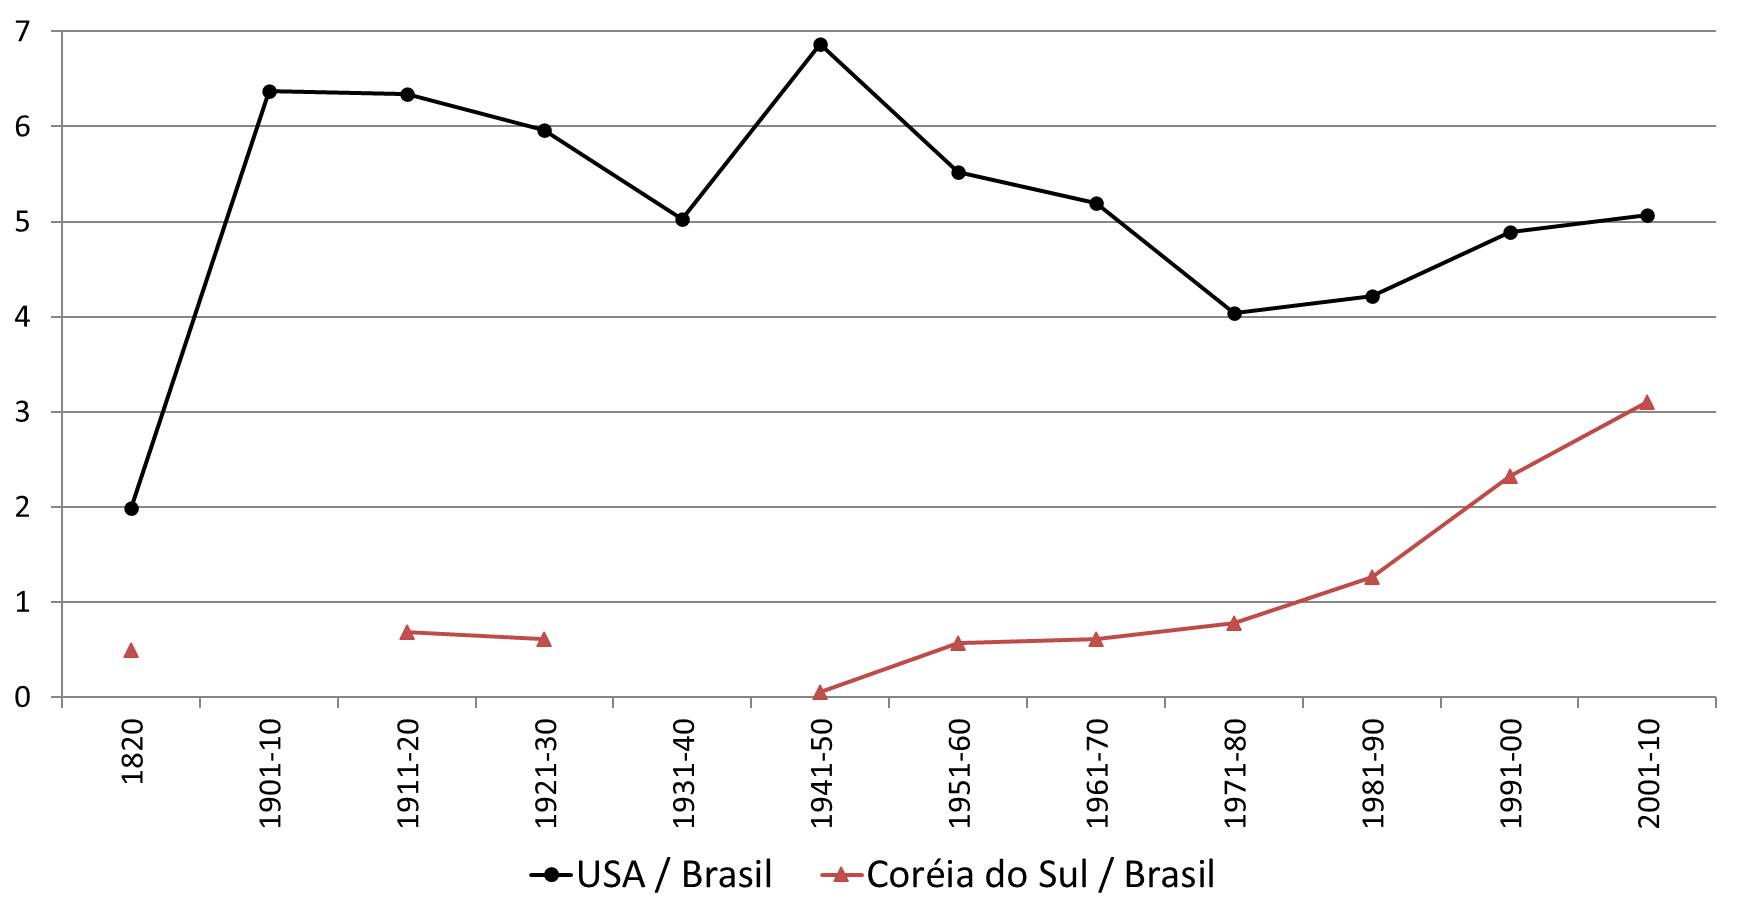
\includegraphics[width=0.7\textwidth]{Imagens/a1i1.png}
\end{figure}

\textbf{Brasil}: \begin{itemize}
    \item Rico ou pobre?
    \item Trajetória de crescimento foi sustentável?
\end{itemize}

\textbf{Como entender a trajetória brasileira}?\begin{itemize}
    \item Diversos grupos ideológicos governaram o Brasil;
    \item Como marca comum, observamos ondas fortes de crescimento;
    \item Essas ondas não mostraram sustentabilidade ao longo do tempo;
    \item E, mais grave, foram sucedidas por graves crises!
\end{itemize}

\subsection{\textbf{Introdução}}
\textbf{O que vamos fazer em HEB II ?}\begin{itemize}
    \item Refletir sobre as escolhas tomadas as longo do tempo e como elas interferiam nesse processo;
    \item Certas escolhas ajudam a explicar esses movimentos;
    \item Mas essas escolhas foram "irracionais"? Ou já "se sabia" que não dariam certo?
    \item Em seu conjunto, elas possuem um certo sentido, uma lógica bem demarcada e um pensamento econômico "adotado" para justificar
    \item Trata-se de uma reflexão fundamental, discussão complexa, nada trivial
    \item Como faremos ? \begin{itemize}
        \item Uma avaliação "técnica"? O que é isso? Quais os guias?
        \item Sim, mas como \textbf{toda} avaliação, ela partirá de uma certa "visão de mundo"; de um certo pensamento econômico;
        \item Referências(ambiente político e econômico) são fundamentais para guiar nossa avaliação dentro de uma certa visão;
        \item Muito relevante ficar atento ao embate entre ortodoxos e heterodoxos (ideias econômicas apoiam e justificam escolhas)
    \end{itemize}
\end{itemize}

\subsection{\textbf{Referências Bibliográficas Políticas}}

\begin{figure}[H]
        \centering
        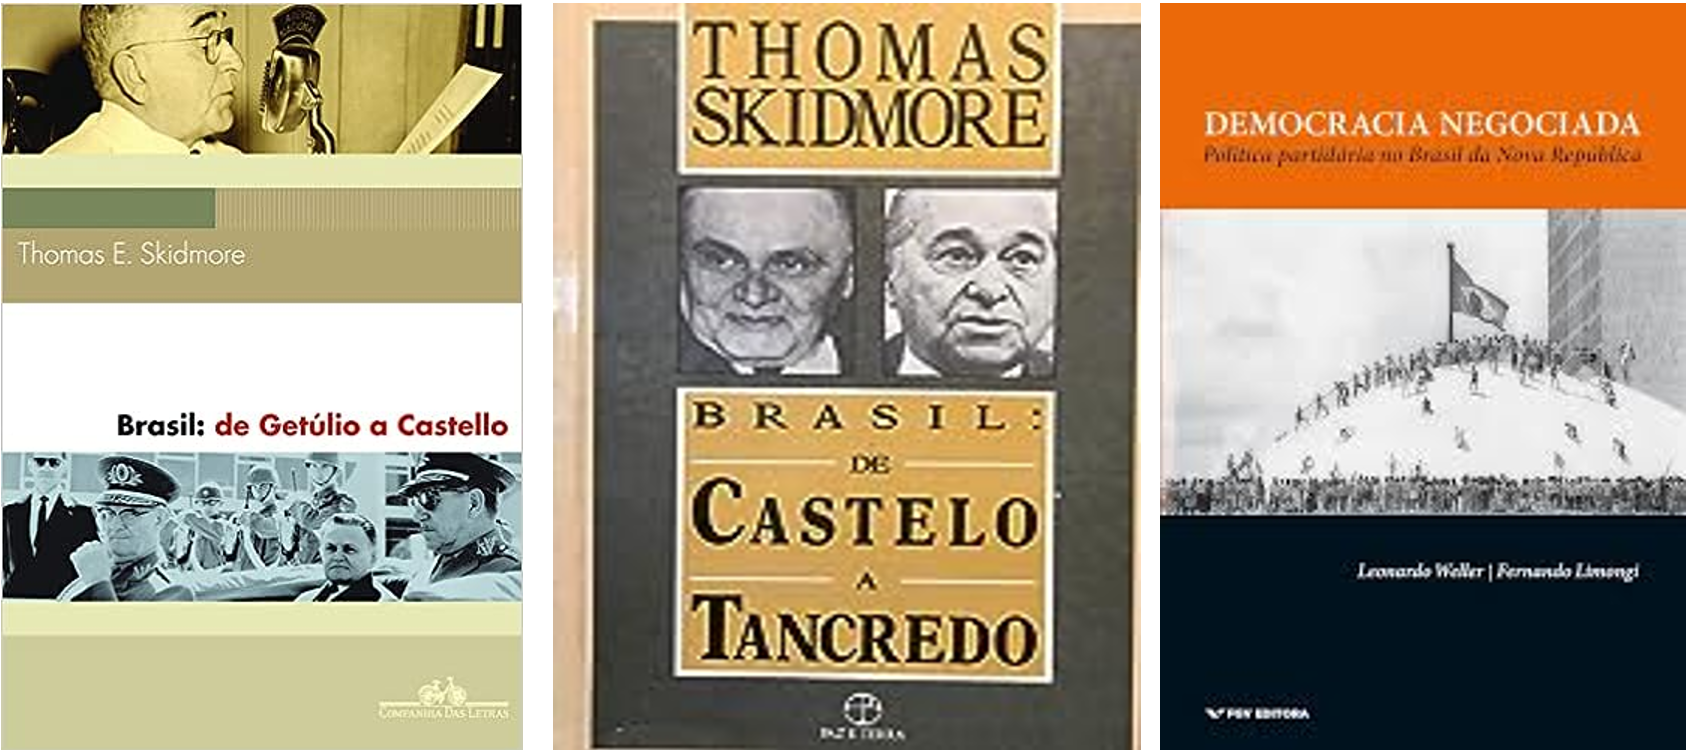
\includegraphics[width=0.7\textwidth]{Imagens/a1i2.png}
\end{figure}

Período democrático: discussões sobre o ambiente político, formação dos partidos e interesses diversos e dinâmica no Congresso Nacional (quando estes eram permitidos). Período não democrático: como os militares e interesses diversos da sociedade participaram desse ambiente

\subsection{\textbf{Referências Bibliográficas Institucionais}}

\begin{figure}[H]
        \centering
        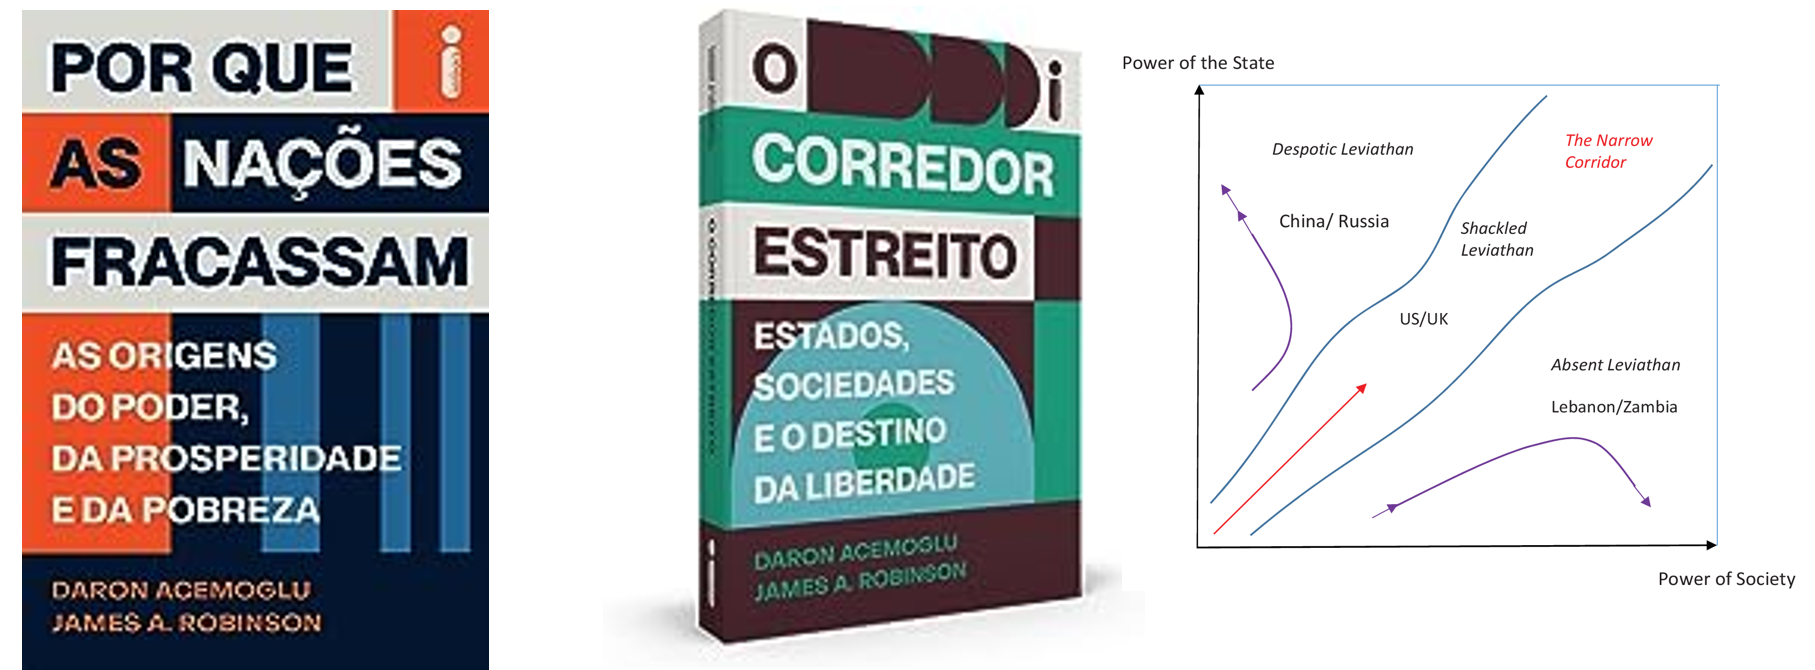
\includegraphics[width=0.7\textwidth]{Imagens/a1i3.png}
\end{figure}

\textbf{Acemoglu e Robinson (2013)}\begin{itemize}
    \item Desigualdade econômica (oportunidades)
    \item Desigualdade política
    \item Instituições extrativistas
    \item Crescimento econômico não sustentável
\end{itemize}

\textbf{Acemoglu e Robinson (2020)}\begin{itemize}
    \item Relação entre Estado e Sociedade
    \item Fundamental ação do Estado – segurança e oportunidades
    \item Fundamental a presença de uma sociedade participativa
    \item Corredor estreito – crescimento econômico sustentável
\end{itemize}

\subsection{\textbf{Política Importa}}
Oque isso significa?:\begin{itemize}
    \item A política nos obriga a pensar sobre a existência de grupos diversos de interesse na sociedade brasileira;
    \item Quais grupos são mais organizados?
    \item Os interesses serão expressos nos governos, nos partidos políticos e no Congresso Nacional;
    \item A política nos obriga a pensar em formação de coalizações governistas; As coalizões são formadas pelos partidos. Os partidos representam os interesses dos grupos sociais
    \item Teremos o desafio de considerar sempre esses aspectos em nossas análises sobre as escolhas econômicas;
\end{itemize}

\subsection{\textbf{Teoria econômica}}
Como a teoria econômica (Acemoglu e Robinson, 2013) explica o caso brasileiro?\begin{itemize}
    \item Sociedade é desigual, isso se reflete na dinâmica política;
    \item O meio político cria instituições extrativistas;
    \item Sociedade como um todo não se beneficia, não percebe a importância de se qualificar, pois não será recompensada;
    \item A sociedade apresenta baixa produtividade, país cresce de forma insustentável;
    \item “Coincidência” tanto governos conservadores ou progressistas tomarem escolhas econômicas em sentido similar?
    \item Elites não desejam formar instituições inclusivas, assim asseguram o controle político;
    \item De modo prático, escolheram regras econômicas que protegem mercados, concede favores tributários e creditícios. Isso acaba deteriorando a competitividade entre os agentes, inviabilizando oportunidades menos desiguais
    \item Exemplo: o gravíssimo problema fiscal atual. Ele é nosso, “compartilhado”. Praticamente, em todas as aulas veremos um exemplo nessa direção extrativista!
\end{itemize}

\subsection{\textbf{Objetivo}}
Discutir e refletir sobre a economia brasileira em perspectiva histórica\begin{itemize}
    \item Tomar posição sobre os problemas econômicos atuais, visando acompanhar/participar do debate nacional;
\end{itemize}

Mas por que pensar em perspectiva histórica?\begin{itemize}
    \item Refletir sobre os problemas/escolhas do passado nos permite acumular aprendizado
    \item Ótima oportunidade para aplicar conhecimento de outras disciplinas de forma mais “prática” (Ex: BP – Macro vs HEB)
    \item Conseguir elaborar boa reflexão e fazer análise robusta exigem muito treino
\end{itemize}

\subsection{\textbf{As escolhas do passado e o presente}}
Escolhas para gerar crescimento econômico trouxeram aumento da renda, mas também problemas

Tentativas de promover o crescimento econômico\begin{itemize}
    \item As escolhas seguiram em qual sentido?
    \item Forneceu um ambiente de negócios atrativo para todos os agentes? Trouxe competição externa aos agentes domésticos? Ofertou educação de qualidade “em massa”?
    \item Não! 
    \item Houve subsídios, interferências no mercado de câmbio, desonerações tributárias para alguns setores escolhidos, menor exposição ao setor externo, crédito favorável etc, para alguns setores; 
    \item ou seja, as medidas foram “verticais” (escolhidos) e não “horizontais” (para todos);
    \item condições desiguais sem contrapartida (com impacto distributivo forte!);
    \item Jogo entre interesses políticos e econômicos resultou a escolha dessas opções! (instituições extrativistas)
\end{itemize}

\textbf{Resultado 1}: progressivamente degradou o ambiente econômico! (instituições)

\textbf{Resultado 2:} houve forte crescimento econômico \begin{itemize}
    \item mas com “prazo de validade”, piora distributiva, crise fiscal, crise da dívida externa e inflação com crescimento explosivo!
    \item “Crescer o bolo e depois distribuir”? O bolo cresceu e a desigualdade também!
    \item desigualdade não importa para o crescimento? O que diz a teoria mais recente?
\end{itemize}

\newpage
\section{\textbf{O periódo do governo JK: política econômica e problemas econômicos}}

\subsection{\textbf{JK, 1956-1961}}
\textbf{Texto: EBC (Cap. 2, trecho sobre JK)}
O que é importante?\begin{itemize}
    \item Notar que seu governo executou um plano direcionado de investimentos. Entender que o plano envolve uma escolha para fomentar o crescimento econômico, via industrialização. Refletir sobre essa escolha.
\end{itemize}

\textbf{Lógica}: transformar o Brasil em um país industrial e urbanizado.\begin{itemize}
    \item Politicamente, a oposição descrevia o governo JK como uma     continuidade de GV; 
    \item Visão estruturalista direciona o discurso econômico para justificar o Plano de Metas\begin{enumerate}
        \item Industria
        \item Instituições
        \item Financiamento
        \item CEPAL
    \end{enumerate}
\end{itemize}

\subsection{\textbf{A reforma cambial de 1957}}
\textbf{Objetivo}: apoiar o Plano de Metas\begin{itemize}
    \item mantida a estrutura de leilões cambiais (priorização de vendas de câmbio, com a intenção de garantir investimentos no país);
    \item criado o CPA (Conselho de Política Aduaneira) para administrar tarifas com foco em acelerar substituição de bens de capital (\textbf{destaque}: setor automobilístico), atrair maquinário moderno para garantir o avanço industrial brasileiro
    \item aplicação da lei do “similar nacional”(um produtor de bem um nacional, semelhante a um bem importado pelo país, pode pedir ao governo o impedimento de entrada desse bem importado, "protegendo" o produtor nacional).
\end{itemize}

A reforma de 1957 avançou a substituição de importações, alavancando a industrialização. Por isso essa reforma foi vista com bons olhos, dado que modernizou a industria brasileira.

\subsection{\textbf{JK}}
A aceleração da inflação em 1957/58, ameaçava o Plano de Metas. \begin{itemize}
    \item Inflação gera incerteza e pode inviabilizar investimentos, isso é isso que o governo ão quer que aconteça, além de reduzir a popularidade dos líderes políticos;
    \item Lucas Lopes (Fazenda) e Roberto Campos (BNDE; "\textit{Bob Fields}"), procuram proporcionar um financiamento adequado para os projetos, essa dupla procurou métodos de financiamento não inflacionário(aumentar tributação, reduzir gastos, atrair investidores) 
\end{itemize}

Plano de Estabilização Monetária (\textbf{PEM}, idealizado por Lucas Lopes e Roberto Campos) lançado em outubro de 1958, seria gradualista (de forma programada a inflação iria sendo reduzida, ou seja, o tratamento seria feito aos poucos e forma pouco agressiva). Mas porque gradualista e não de choque? Esse plano gradualista garantiu que o avanço da industria e investimento não fosse afetado de maneira agressiva. E mesmo assim o \textbf{PEM} afetou o plano de metas. 

Por que o PEM entrou em confronto com o Plano de Metas? O investimento acabou sendo reduzido, gerando a necessidade de uma emissão monetária para financiar o desenvolvimento 

Como encarar a inflação? (gradualismo, a inflação, nessa época, um mal necessário, pois no futuro, o desenvolvimento da industria/economia iria "compensar")

Qual foi o desfecho desse confronto?\begin{itemize}
    \item O custo de desinflacionar(PEM) foi maior do que conviver com a inflação(Plano de metas). Chegou ao fim o \textbf{PEM} devido ao alto custo que o \textbf{PEM} exigia do Plano de Metas, e o JK(ou melhor, quem ele representava) não queria de o Plano de Metas acabasse.
\end{itemize}

\subsection{\textbf{Banco do Brasil e a tendência inflacionária}}
Principais atores do sistema financeiro brasileiro (SFB):\begin{itemize}
    \item - SUMOC (regulador, o “Bacen” da época, Superintendência da Moeda e do Crédito), BB (Camob, Cacex e CARED) e Tesouro Nacional (Caixa de Amortização, o cara que imprime a moeda).
\end{itemize}

O desenho do SFB era bom, mas...\begin{itemize}
    \item O Banco do Brasil(\textbf{BB}) é banco do governo e banco comercial (Uma linha de crédito pode ser conflitante com uma política monetária restritiva); 
    \item Há dois canais de vazamentos da política monetária, isto é, duas fontes de expansão de moeda. Se é tão ruim, porque isso nunca foi arrumado? Isso não é tão simples quanto parece.
\end{itemize}

\subsection{\textbf{Vazamentos da política monetária}}
\begin{enumerate}
    \item De criação de papel moeda\begin{itemize}
        \item Tesouro de Amortização emite moeda(mas não a põem em circulação), mas quem coloca em circulação é o BB via CARED; 
        \item Isso se mistura com a concessão de créditos subsidiados, por ex, para Agro e Ind(os setores que mais demandavam crédito e sempre cada vez mais); e empréstimos feitos para "pessoas físicas" $\Rightarrow$ E assim uma política monetária expansionista surgiu
        \item havia limite de financiamento feito pelo Congresso, mas sempre era ampliado pelo Congresso; Lembrando que o congresso nacional era pressionado(por grupos da sociedade) para aumentar mais ainda a emissão monetária, o \textbf{BB} também era pressionado por pessoas que queria linhas de crédito 
        \item BB causador irracional de inflação? Há interesses, o \textbf{BB}+Congresso eram "obrigados"!
    \end{itemize}
    \item De transformar moeda escritural (depósitos bancários) em base monetária(isso gera expansão da base monetária e o resultado é o mesmo) \begin{itemize}
        \item Temos as reservas compulsórias e as voluntárias. Um banco comercial pode expandir crédito, utilizando as voluntárias, mas claramente possui seu limite dada sua captação, tamanho e estratégia de fornecer crédito.
        \item Mas o BB pode expandir de forma ilimitada. É ele quem acolhe os compulsórios dos bancos comerciais. Ele pode creditar a reserva, pois o credor é ele mesmo!
        \item na prática: BB transforma moeda escritural (depósitos bancários) em base monetária, alimentando, por ex., o crédito! Irresponsável? Mais uma vez, interesses!
    \end{itemize}
\end{enumerate}

Por isso é tão difícil arrumar esses vazamentos monetários que geraram a expansão fiscal e por fim o aumento da inflação.

\subsection{\textbf{Tendência inflacionária}}
BB como banco comercial e do governo + Vazamentos da política monetária(por grupos influentes e demandantes de capital) + Pressões dos agentes econômicos e políticos = tendência inflacionária\begin{itemize}
    \item essa equação ilustra e explica a tendência inflacionária;
    \item permitiu financiar o Plano de Metas;
    \item Os vazamentos disponibilizavam recursos (gastos para o governo($\uparrow g$) e  crédito subsidiado para o setor privado(empréstimos baratos fornecidos pelo \textbf{BB}));
\end{itemize}

Ou seja, a fonte de recursos do Plano de Metas tinha origem de uma “poupança forçada” (um apelido da inflação)


\subsection{\textbf{Plano de Metas}}

Conselho de desenvolvimento (ligado à presidência e ao BNDE) elaborou 30 metas, englobando 5 áreas (energia, transporte, indústrias de base, alimentação e educação) + construção de Brasília\begin{itemize}
    \item Com orçamento de 5\% do PIB;
    \item Setor privado (nacional e estrangeiro) direcionou para automobilístico, construção naval, mecânica pesada e equipamentos elétricos;
    \item Dependeu da adoção de tarifa protecionista em conjunto a um sistema cambial que subsidiava importação de bens de capital, insumos e atrairia IDE
    \item financiamento seria “viabilizado” ao longo da execução do Plano. A participação maior ficou a cargo do setor público, via participação ativa do BB e Tesouro Nacional
\end{itemize}

\textbf{Síntese}: um PSI com estratégia baseada em economia fechada, liderança do Estado e setor privado fortemente beneficiado


\begin{figure}[H]
    \centering
    \caption{Plano de Metas: previsão e resultados   1957 – 1961}
    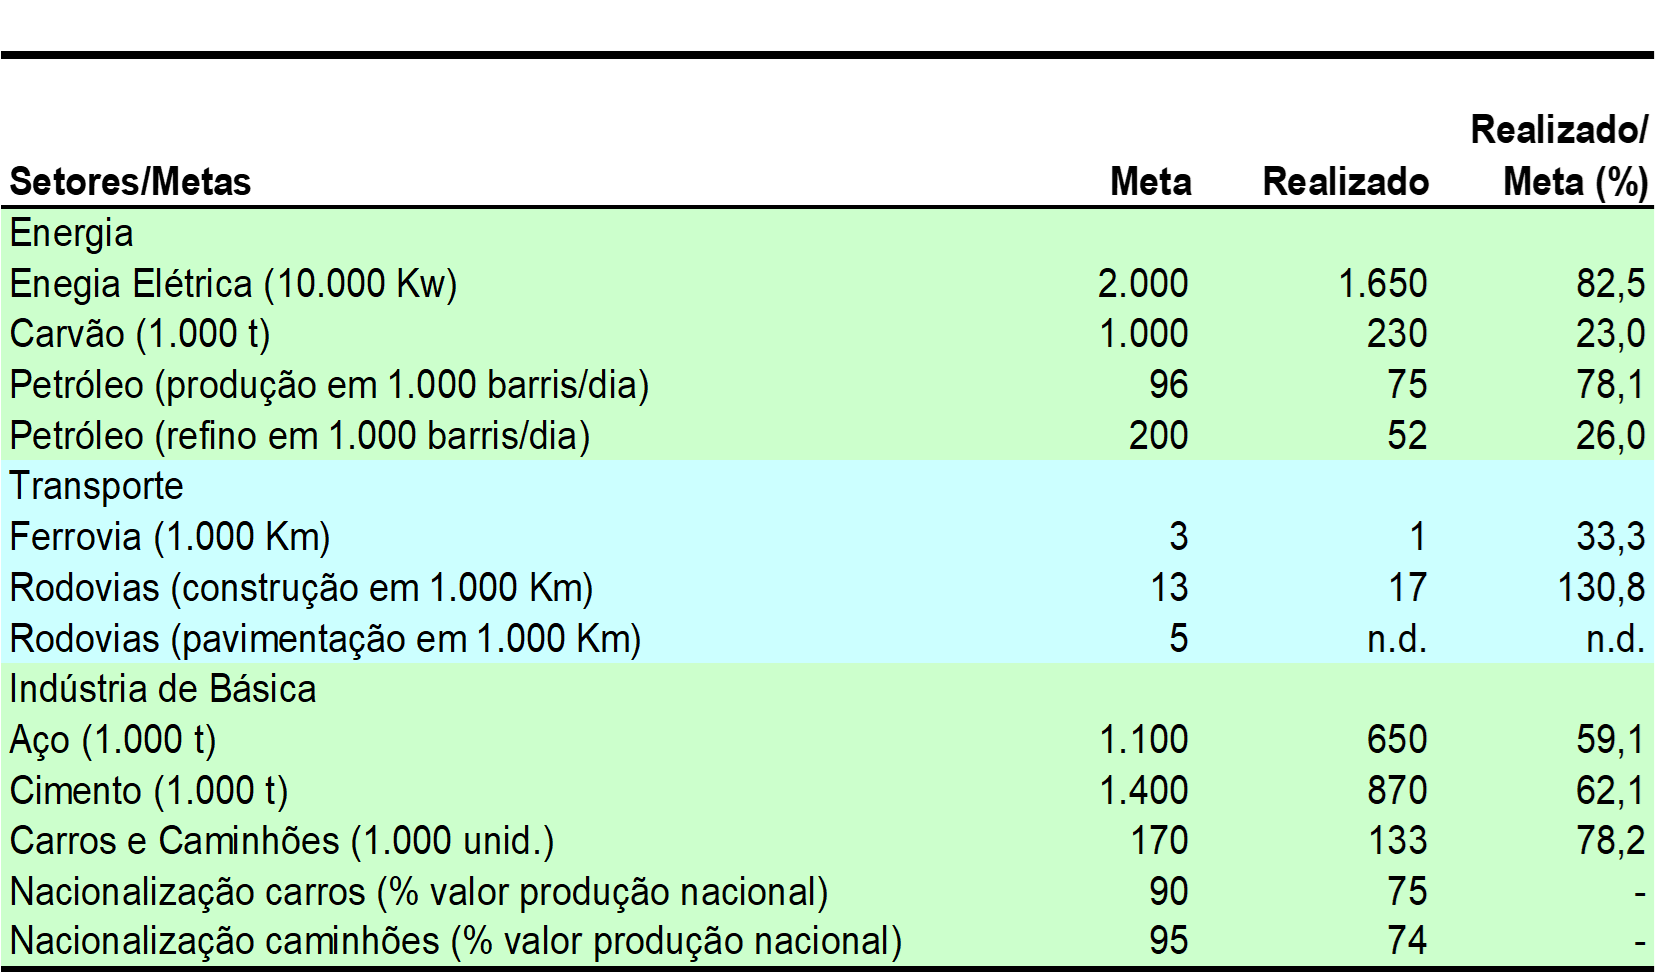
\includegraphics[width=0.7\linewidth]{Imagens/a2i1.png}
\end{figure}

Das metas definidas, grande parte das metas não foram alcançadas. O investimento na parte de transporte, como desenvolvimento das rodovias e a logística. Desenvolvimento da cadeia energética e das cadeias básicas de suprimento(aço). Enquanto a nacionalização de carros, se trata de carros produzidos no Brasil, devem ser feitas usando peças que foram produzidas nacionalmente(não o fato de carro ter sido feito no Brasil), isso se trata da indústria de \textbf{auto-peças}, a base da indústria automobilística. 

A industria de \textbf{auto-peças} movimentou muito o desenvolvimento das cidades e economia brasileira.

\subsection{\textbf{Plano de Metas: uma síntese}}

Pensamento econômico (CEPAL(grupo de pesquisadores latino-americanos preocupados com o desenvolvimento nacional e propuseram ideias para o desenvolvimento, empresas latino americanos precisam se desenvolver via industrialização para se equiparar a países mais avançadas); Estruturalistas)\begin{itemize}
    \item Importância da industrialização (crescer sem causar inflação de médio e longo prazo e crise cambial) como a industria de auto-peças, que dispensaram a necessidade de importação;
    \item Como? Política de Substituição de Importações, economia fechado no curto prazo e fornecendo capital para os setores privados potenciais via incentivos(proteção de mercado) e créditos baratos, somente o mercado interno era atendido.
\end{itemize}
    
Escolha de um setor\begin{itemize}
    \item Efeitos setoriais em cadeia; Incentivo de industria de base para outras.
    \item Logística; modal rodoviário para todos os lugares do Brasil.
    \item Urbanização.
    \item Regra de Conteúdo Local(\textbf{RCL}); Subsídio para o setor privado desde que o mesmo setor privado compre insumos nacionais.
\end{itemize}

Participação do Estado, setor privado e investidores estrangeiros; Industria internacional com fábrica no Brasil(investidores estrangeiros) + Fornecimento de insumos básicos  para essas industrias grandes(setor privado) + Escolhe de setor junto de incentivos para essas grandes industrias(Participação do Estado).

E o saldo do Plano de Metas?\begin{itemize}
    \item Forte crescimento econômico e impactos produtivos significativos; Delicado isso(desenvolveu sua economia de grandes proporção junto de um grande desenvolvimento interno, porém com um custo elevado da inflação).
    \item Faltou sustentabilidade (crises no início dos 1960, inflação, dívida pública(interna e externa) e reforço do extrativismo(instituições extrativistas; setores escolhidos a dedo para receber benefícios e sociedade pagou o preço)).
    \item Grupos brasileiros se aproveitaram desse boom econômico financiado pelo governo.
\end{itemize}

\section{\textbf{O período dos Governos de Jânio Quadros e João Goulart}}

\subsection{\textbf{Introdução}}
No período de 1961 até 1964 temos uma renúncia, uma experiência parlamentarista e rompimento do regime democrático\begin{itemize}
    \item ambiente político instável, incerteza política
\end{itemize}

Jânio Quadros assume em janeiro de 1961 com forte votação, apoiado por conservadores (UDN) e por suas propostas de cunho populista.\begin{itemize}
    \item Mas não tinha maioria no Congresso. O que dificultava o avanço de processo, e para realizar avanços, precisava de realizar coalizações e atender interesses internos do congresso
\end{itemize}

Em suma:\begin{itemize}
    \item politicamente frágil desde o início do mandato;
    \item economicamente, herdou o contexto macro difícil pós JK (Inflação, déficit público elevado e deterioração das contas externas).
\end{itemize}

\subsection{\textbf{Quadros, 1961}}

Estratégia: promover estabilização inflacionária e recuperar o crédito externo\begin{itemize}
    \item Aplica medidas ortodoxas e promove forte desvalorização cambial, com a intenção de alterar os preços relativos para tentar melhorar a balança comercial via melhoria das exportações.
\end{itemize}

Em 1961, a SUMOC, estabelece a \textbf{Instrução 204}(fim do sistema de leilão de câmbio)\begin{itemize}
    \item unifica o mercado de câmbio(o mercado de câmbio vai sofrer menos intervenção, algo que vai de acordo com a mentalidade do Quadros, fim da intervenção estatal sobre esse mercado), promovendo menor necessidade de recursos para cobrir subsídios cambiais; lembrando que toda intervenção é quando uma ação governamental interfere em algum mercado, alterando as "forças" que definem o mercado.
    \item reduz subsídios às importações;
    \item na prática, era o fim dos leilões cambiais;
    \item Como o cenário era de divisas reduzidas, câmbio ficou pressionado no sentido da desvalorização
\end{itemize}

Medidas são bem recebidas pelo FMI(órgão que observa movimentações política-monetárias e isso gera boas ou más reputações sobre economias) o que permite renegociar a dívida externa devido as "boas práticas" de redução da intervenção do governo sobre o mercado de câmbio.

O governo manteve as metas monetárias e creditícias(JK havia rompido com isso em seu governo), estabelecidas com o FMI(mais um motivo para o FMI ver o Brasil com melhores olhos), visando controlar o déficit público e a inflação. 

Mas a inflação não retrocedeu , apesar das medidas contracionistas e liberais. Por que?\begin{itemize}
    \item A economia estava super aquecida devido as políticas super-expansionistas de JK
    \item Políticas monetárias e fiscais adequadas para controle de inflação não geram resultados imediatos, ainda mais em um governo que durou menos de um ano
    \item Houve desvalorização cambial, portanto, repasse cambial, gerando uma inflação mais persistente ;
    \item A demanda agregada estava bastante aquecida.
\end{itemize}

Jânio, de forma “surpreendente”, renuncia em agosto de 1961, colapsando total a tentativa de estabilização\begin{itemize}
    \item De fato, não conseguiu viabilizar uma coalização de forças para gerir os interesses diversos presentes na economia política
\end{itemize}

\subsection{\textbf{Jango, 1961-1964}}

Militares \textit{"vetaram"} a posse do vice, Jango (PTB-RS; que foi eleito em uma chapa mista, e o Jango era opositor de Quadros, tanto em ideias quanto em atitudes(ele era trabalhista e não populista)), levando à adoção do Parlamentarismo junto da presidência do Jango (por conta do receio/desgosto do congresso em relação Jango)(set. 61 - jan. 63).
    
O primeiro-ministro apresentou, no campo econômico, uma carta de \textit{"boas intenções"}:
    \begin{itemize}
        \item Não prometeu quando ou como, mas prometeu o que ele iria fazer, isso era a carta de boas intenções 
        \item Diante da aceleração inflacionária, medidas contracionistas foram tomadas em set. de 1961.
        \item Ainda assim, o fim de 1961 mostra piora do déficit público e crescimento da expansão monetária.
    \end{itemize}

Preocupações: controlar inflação e realizar plebiscito sobre o parlamentarismo, ele de forma indireta/paralela, consegue retornar ao controle executivo e tomar controle das políticas fiscais para conduzir o Brasil para um bem estar

\textbf{Política Econômica}

Anunciado ao fim de 1962, o Plano \textbf{Trienal} de Desenvolvimento Econômico e Social (coordenação de \textbf{Celso Furtado}; o maior representante brasileiro da CEPAL, logo medidas heterodoxas(medidas mais intervencionista e radicais)).

\textbf{Objetivo}: conciliar crescimento econômico com reformas sociais e combate à inflação, isso é uma medida bem ortodoxas(indo contrário da forma de pensamento de Furtado, apesar de ser orquestrado por ele e ele tinha consentimento disso pois sabia que isso traria benefícios futuros).

\begin{itemize}
    \item Parte de um diagnóstico tradicional e centra-se em medidas ortodoxas (boa negociação com FMI seria importante);
    \item Inflação tinha origem na forte expansão de gastos públicos;
    \item Mas, também, apresenta medidas heterodoxas.
\end{itemize}

\subsection{\textbf{Jango (presidencialismo)}}

Instruções 234 (para o BB) e 235 (para bancos privados) da SUMOC são adotadas para restringir a expansão do crédito(medida ortoxas);

Impõe “realismo tarifário (redução de subsídios à importação e aos serviços públicos de transportes e comunicação) e cambial”; 

Fim dos subsídios com consequentes aumentos de preços de trigo e petróleo enfrentam resistência na base de apoio ao governo: sindical e parlamentar;

Meta audaciosa 7\% de crescimento econômico com redução gradualista da inflação (50\% em 1962 para 10\% em 1965);

Acordos de congelamento de preços são “combinados”(forçado) com alguns setores (aspecto heterodoxo(forçando a não mudança de preço para não afetar a inflação));

\subsection{\textbf{Quais foram os resultados do Plano Trienal?}}

Pressões de certos sindicatos sobre o governo.

Houve elevação de preços industriais (provavelmente uma reação dos agentes, esperando um controle de preços, antecipam aumentos). Reação ao congelamento de preços de outros setores antes que chegue no seu setor. Reação dos agentes do mercado sobre as medidas heterodoxas (antecipação de aumento de preços antes do seu congelamento)

Plano inconsistente(suas ideias eram conflitantes): metas de redução de inflação, ao mesmo tempo  forte tarifação e congelamento.

Perda generalizada da base política do governo (industriais, sindicatos, Congresso...). Base do governo taxava as medidas de recessivas. 

Em maio de 1963, o Plano já começa a ser abandonado. 

Jango apoia elevação salarial(indo no sentido contrário do congelamento de preços feito no Plano Trienal), contrariando a estabilização e inviabilizando o acerto das contas públicas e as negociações com o Fundo. O governo está por um fio. 

Recessão tem início em agosto(lá se foi o último fio que mantinha o governo).

\subsection{\textbf{A recessão de 1963 foi causada pelo plano Trienal?}}
    
Primeira recessão desde 1943, sendo sequência de um plano de estabilização do governo João Goulart! Uma história que está bem orquestrada.

\begin{itemize}
    \item Seria o esgotamento da PSI (Política de Substituição de Importações ;C. Furtado e M. C. Tavares);
    \item Aceleração inflacionária e turbulência política (M. H. Simonsen, de acordo com Simonsen a incerteza inflacionária e política culminou na recessão de 63 no Brasil, bem inspirado na tese de Friedman que o aumento da inflação, gera maior incerteza inflacionário, essa maior incerteza gera maior recuo dos agentes econômicos);
    \item Queda da poupança pública e piora do setor externo; \textit{"disputa"} com FMI afasta investimento estrangeiro com efeito negativo sobre a confiança do empresário nacional; sequência de planos de estabilização com contenção da demanda deixaram somente os custos (M. Mesquita). Além disso mostra que o Brasil tem impaciência sobre políticas de desinflação.
\end{itemize}

\textbf{Mas:}
\begin{itemize}
    \item Difícil responder com poucas informações em base trimestral; por isso é difícil de gerar uma relação de causa e consequência entre o plano trienal e a recessão.
    \item Explicações acima não se apoiam em datação cíclica trimestral;
    \item O Plano Trienal foi lançado em dezembro de 1962 e abandonado em maio de 1963. A recessão começa no 3º trimestre de 1963;
    \item Cenário instável no ambiente político desde 1961 e custos da inflação parecem ter influenciado.
\end{itemize}

Quem explica a recessão de 1963, dado a primeira aula da HEB II ?? $\rightarrow$ A depender das instituições que governam a economia, teremos desenvolvimento ou não da economia, dado que o Brasil apresentou instituições extrativas e gerou a nossa recessão em 1963. \textit{Daron Acemoglu} explica

\subsection{\textbf{Jango e a mudança do regime político}}

Em suma: baixo comprometimento com medidas, fraco apoio político e metas não cumpridas de estabilização.

O fim de 1963 mostrava inflação a 80\% e forte desaceleração econômica\begin{itemize}
    \item partidos conservadores conseguiram mobilizar grandes passeatas no início de 1964; elite econômica descontente;
    \item em 31 de março um movimento militar com amplo apoio do empresariado, classe média, imprensa e maioria parlamentar fechou a terceira república.
\end{itemize}
\newpage

\section{\textbf{O período do governos Costa e Silva e Médici: “Milagre econômico”}}
\subsection{\textbf{Introdução}}
Identificar e refletir sobre os determinantes do milagre econômico do Brasil, avaliando suas conexões com o setor externo, a inflação e a industrialização.

\subsection{\textbf{Costa e Silva e Médici, 1967-74}}
Contexto político (“anos de chumbo”):\begin{itemize}
    \item Castello Branco foi sucedido por Costa e Silva em 1967 e na sequência Médici em 1969.
    \item Decretado o AI-5 (dez/1968) – fechou o Congresso, suspendeu garantias constitucionais, perseguiu opositores do regime e ampliou forte o intervencionismo do Estado na economia.
    \item Em 1968, o Brasil, de fato, deixou de ser uma democracia e se tornou um regime altamente restrito e opressor em relação a divergências com os ideias daqueles no poder
\end{itemize}

Conduzido pelo Ministro da Fazenda Antônio Delfim Netto.

\subsection{\textbf{Milagre econômico}}
Marcas do “milagre econômico” brasileiro:\begin{itemize}
    \item Brasil cresceu na média 11,2\% (máximo de 14\% em 1973, média histórica no pós Guerra foi 7\% ); O Brasil no seu momento de crescimento "chinês"
    \item Crescimento do setor industrial foi ainda mais forte do que essa média de crescimento geral; 
    \item Taxas de inflação foram declinantes e relativamente baixas para os padrões brasileiros; em comparação com outros períodos, crescendo de maneira forte e acelerada acompanhada de inflação baixa e controlada (um sonho que qualquer economia)
    \item Houve superávits no balanço de pagamentos neste período(em comparação com os períodos anteriores). Brasil começou a ter um aumento expressivo nas reservas internacionais.
\end{itemize}

Mas como explicamos esses resultados?\begin{enumerate}
    \item Decisões políticas de alto controle levaram a isso?
    \item Período de grande desenvolvimento global e Brasil se aproveitou disso?
    \item Consequências do PAEG?
\end{enumerate}

\subsection{\textbf{Os determinantes do milagre econômico}}
A política econômica do período 1968-1973 \begin{itemize}
    \item políticas monetária e creditícia expansionistas e os incentivos às exportações.
\end{itemize}

O ambiente externo favorável \begin{itemize}
    \item grande expansão da economia internacional, gerando melhoria dos termos de troca e crédito externo farto e barato para o Brasil.
\end{itemize}

As reformas institucionais do PAEG, em particular as reformas fiscais/tributárias e financeira\begin{itemize}
    \item criaram as condições para a aceleração subsequente do crescimento.
\end{itemize}

\subsection{\textbf{Plano Estratégico de Desenvolvimento (PED), Plano Governamental }}
Lançado em meados de 1968, mas visando o desenvolvimento igual sempre\begin{itemize}
    \item expandir setores de bens de capital (indústrias mecânica e elétrica  e de bens intermediários –siderurgia e metalurgia do alumínio); Foco em desenvolvimento industrial
    \item utilizar o potencial de crescimento do setor de bens de consumo duráveis, graças à elevada elasticidade-renda do setor; [ex: geladeira, fogão, TV; conhecido como "linha branca", bens de consumo duráveis]; algo padrão em países que estão passando por um período de urbanização, apesar de serem itens de alto custo, o governo forneceu linhas de créditos para que incentive o consumo desses bens.
    \item Ainda existia importações de certos bens, mas setores estratégicos(algo escolhido pelo governo) era exclusivo de investimento e consumo nacional.
    \item consolidar a infraestrutura (função do governo); Ainda a rede de transportes como rodovias, ferrovias e hidrovias deixavam a desejar e o governo deveria arrumar isso.
\end{itemize}

Política de minidesvalorizações cambiais, \textit{crawling peg} (corrigir inflação para não prejudicar a balança comercial; isso era feito para proteger as exportações/exportador da inflação doméstica(caso ela cresça mais que a internacional), logo usava o câmbio como um amortecedor para o câmbio real); Isso não nasceu com Delfim Netto(mas usou bastante), isso foi descido no governo anterior e isso era uma política que foi instituída dentro do PAEG também.

Lei no 4.131(também criada dentro do \textbf{PAEG}), empresas nacionais terem acesso direto ao sistema financeiro internacional;

Resolução 63 do Bacen(também criada dentro do \textbf{PAEG}), bancos comerciais nacionais podem captar recursos externos e repassar ao mercado interno(empresas e clientes).

Delfim Netto aproveitou muito das implementações do \textbf{PAEG}. O mundo deixou de ter uma escassez de dólares e passou a ter um abundância de dólares, e o Brasil se aproveitou dessa sobra de capital para ao aumentar o mercado nacional(ainda mais com o juros relativamente baixas e interessantes para o mercado de crédito nacional, gerando crescimento de longo prazo). O \textbf{PAEG}(ou melhor as regas dentro dele) de certa forma influenciou o resultado do milagre econômico.

\subsection{\textbf{Milagre econômico e industrialização}}
Políticas governamentais setoriais específicas:\begin{itemize}
    \item crédito com taxas subsidiadas(Brasil sendo o Brasil) concedido por autoridades monetárias(por exemplo o Banco do Brasil) para o setor agrícola(que alegava importância nacional e internacional); O agro toma crédito não só para se preparar para próximas safras, mas sim para se modernizar e aumentar sua produtividade, isso incentivou o desenvolvimento de maquinários mais eficientes e isso fomentava a indústria de máquinas, com o aumento da produtividade, há um aumento da oferta, esse aumento da oferta gera impacto na inflação. Logo o \textbf{PED} influenciava na inflação. Mas esse aumento de oferta vai também para as exportações. Logo o \textbf{PED} também influenciava as exportações. Isso não é uma mentalidade cepalina, por mais que seja medidas estruturalistas, mas o desfecho, os meios e os desejos são cepalinos, mas isso não é uma visão cepalina.
    \item mecanização agrícola gera demanda por produtos industriais, assim como fez a Política Nacional de Habitação(setor imobiliário); Resultado do \textbf{FGTS}(que era uma poupança obrigatória) o que auxiliou as linhas de crédito.
    \item há incentivos para setores exportadores tradicionais como têxteis e calçados; eles já tem uma contribuição na balança comercial, e os governos vão querer aumentar a participação deles na balança de comercial. Para aumentar esse desenvolvimento, usamos da mesma ferramenta, linha de crédito. E um crescimento desses setores gera empregos.
    \item grande expansão de crédito, criando sociedades de crédito e de investimentos (\textbf{PAEG} – reforma financeira) que forneceram crédito direto ao consumidor.
\end{itemize}

\subsection{\textbf{Inflação}}
Diagnóstico: “Inflação de custos; a culpa do processo inflacionário vem desse aumento de custos”\begin{itemize}
    \item foco na “inflação de custos”(Delfim Netto quem eliminar o "mal" pela raiz), especialmente o custo do crédito;
    \item incentivos tributários, subsídios de juros e créditos subsidiados facilitados e menores (juros; quanto mais o juros, maior o custo financeiro, quanto maior o custo financeiro maior o repasse para os preços e o aumento de preço gera inflação) foram amplos para o setor agrícola e industrial, chave no sentido de reduzir pressões inflacionárias e de gerar divisas para o país. E já vimos a cadeia de consequências(produtividade, oferta, inflação, câmbio, exportações e balança de pagamento, tudo isso para propiciar o crescimento econômico sustentável).
    \item Delfim Netto quer algo (crescimento econômico sustentável) mas fazer isso de forma "irracional" gera consequências que impedem esse algo (inflação + política monetária contracionista), para fazer isso do jeito certo tem um processo lógico de uma cadeia de produção e oferta, trazendo uma segurança e estabilidade para alcançar esse algo. É isso que ele vêm fazendo de certa forma.
\end{itemize}

\subsection{\textbf{Inflação e o milagre}}
Questão fiscal(olhando para inflação em declínio, junto de um forte crescimento econômico, créditos subsidiados e a pergunta é simples , como? Tá sabemos o resultado, inflação em queda, mas como isso ocorreu)\begin{itemize}
    \item Resultados fiscais(olhando para o deficit primário) e financiamento do déficit \(\rightarrow\) ele era controlado e muito bem acompanhado e quando necessitava (\textbf{PEG} age de novo), emissão de títulos públicos, logo há uma contribuição positiva(no sentido de não gerar processo inflacionários descontrolados). 
    \item Subsídios, Estatais e o Orçamento monetário(criado nesse governo; estrutura contábil para despesas financeiras(juros) das estatais que tomavam empréstimos e subsídeos) \(\rightarrow\)Essas três despesas não entravam na conta dos resultados fiscais primários, olhando o para o resultado primário , a inflação não acelerava, mas olhando em conjunto com o Orçamento Monetário, vemos políticas fiscais expansionistas, levando a processos de aceleração inflacionário. Ok , mas porque a inflação não estva crescendo então?
\end{itemize}

Intervencionismo: houve controle compulsório dos preços (CIP; Conselho Interministerial de Preços)\begin{itemize}
    \item Congelamento generalizado(de diversos setores) dos preços(câmbio, juros, bens e serviços dos setores privado e público). Reajustes com base nas variações de custos. O Governo de controlava isso, via cálculos de planilhas e planilhas de dados para saber qual vai congelar e qual pode subir. Logo os índices inflacionários ficavam também "congelados" de certa forma, logo a inflação também.
\end{itemize}   

Dinâmica cambial (setor externo favorável; \textit{crawling peg}), além disso havia uma entrada grande dólares na economia, o que auxiliava na redução das pressões cambias e portanto na inflação em redução.

Política salarial (persiste o achatamento salarial desde o \textbf{Paeg}; formulação salarial, derretimento/achatamento salarial), isso gera redução da inflação.

Capacidade ociosa(na industria isso é maquinário parado, ociosidade industrial) da economia brasileira desde 1964, havia , de certa forma, espaço para o Brasil crescer sem gerar pressões de aceleração inflacionária, pelo menos no primeiro momento.

Políticas setoriais e inflação (caso do Agro)

Resultado líquido (“curva de Phillips achatada”)\begin{itemize}
    \item Inflação foi declinante no período do Milagre
    \item Tem espaço para crescer mais até gerar pressões inflacionárias.
    \begin{figure}[H]
        \centering
        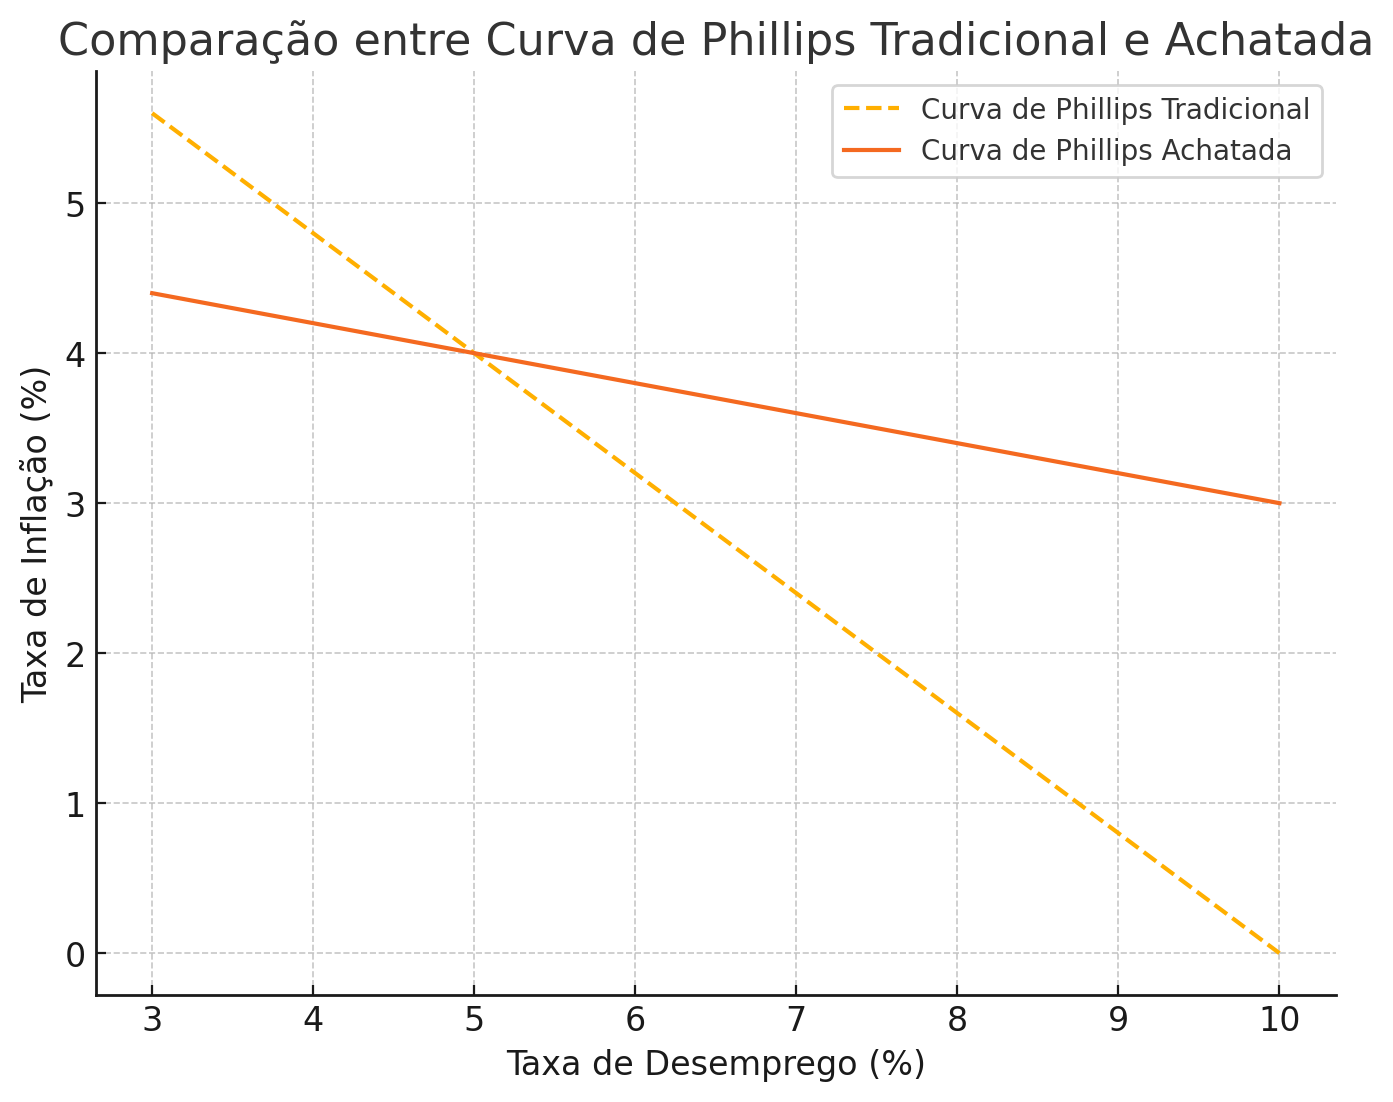
\includegraphics[width=0.7\linewidth]{Imagens/a4i3.png}
    \end{figure}
\end{itemize}

Houve jornais da época alegaram e pesquisas recentes comprovaram que havia preços artificiais (preços coletados de maneira não aleatória e viesado).

\begin{figure}[H]
    \centering
    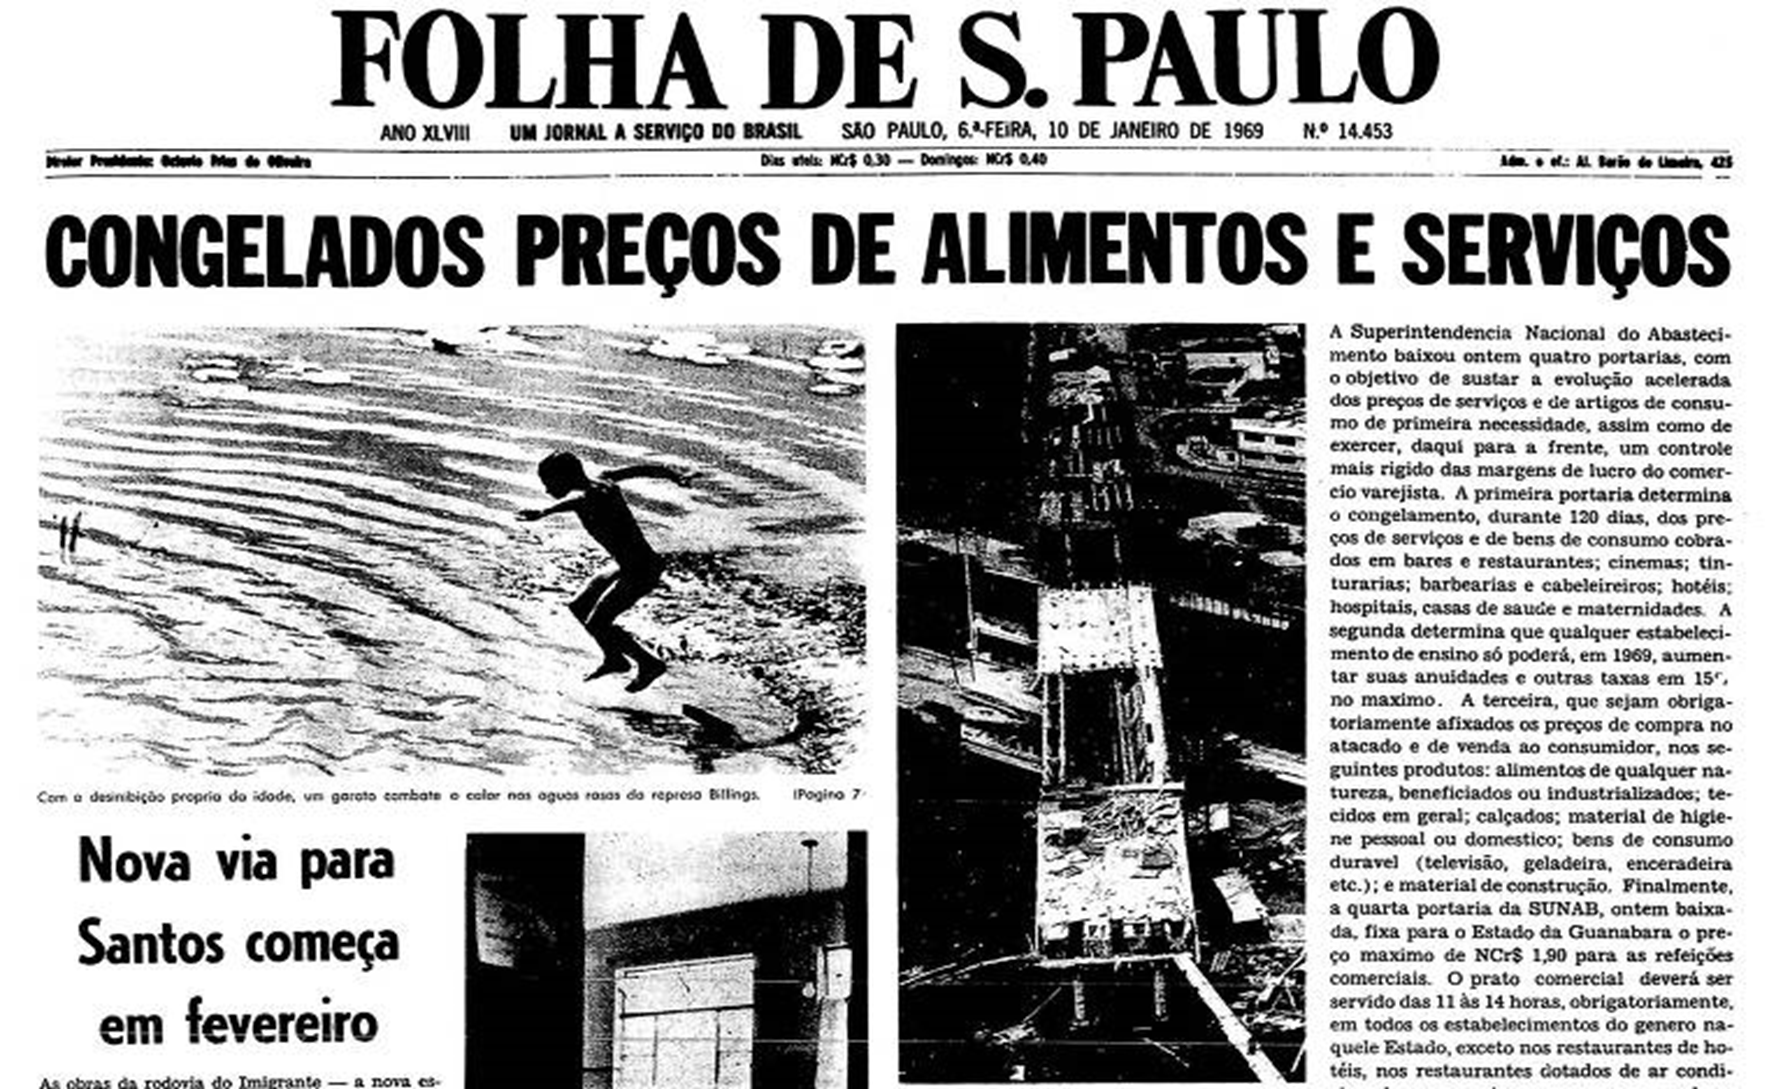
\includegraphics[width=0.7\linewidth]{Imagens/a4i1.png}
\end{figure}

\begin{figure}[H]
    \centering
    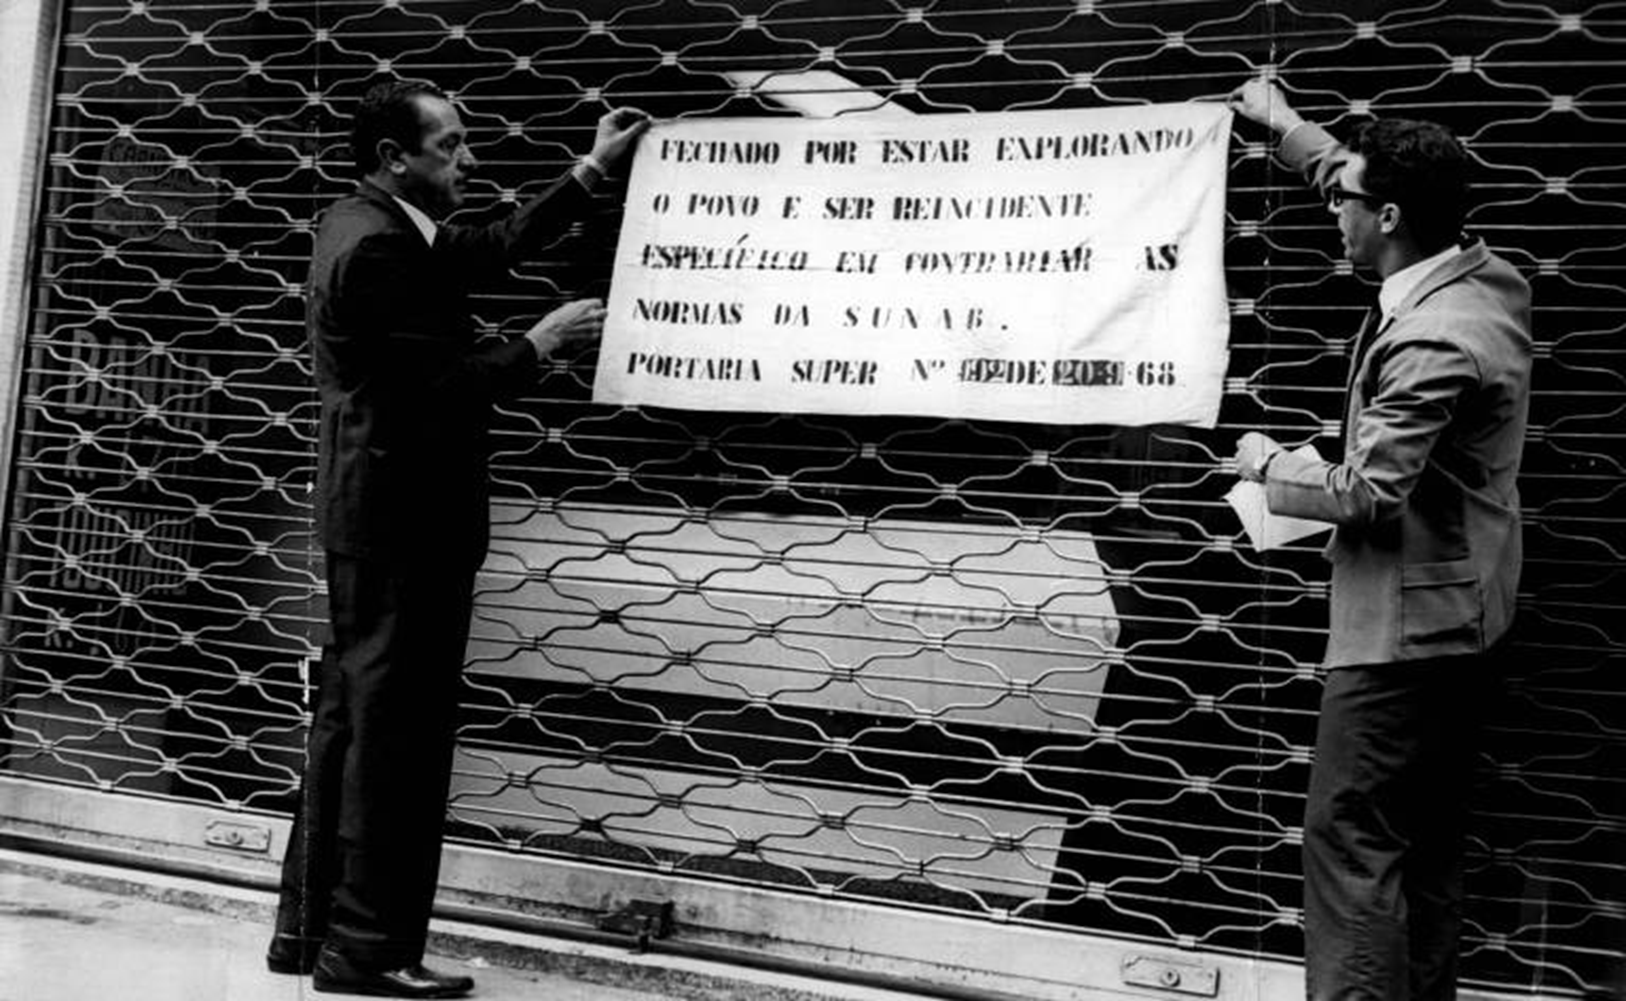
\includegraphics[width=0.7\linewidth]{Imagens/a4i2.png}
\end{figure}

\subsection{\textbf{Setor externo}}
BC(\(BC=EX-IM\)) “equilibrada” (exportações e importações cresceram bastante)\begin{itemize}
    \item Exportações (incentivos para o setor privado) e importações (continuidade da industrialização)
    \item Crescimento global e termos de troca favoráveis
    \item Minidesvalorizações cambiais
\end{itemize}

BS/R (Balança de servços e renda;o serviço da dívida(juros da dívida externa, transferência de dividendo, lucros) externa começa a se elevar) essa conta , nesse momento, ela vai ser be negativa, dada as atividades.

CK(Conta de Capitais: entrada de recursos de não residentes;"empresas estrangeira vem investir no Brasil";Dívida) superavitária\begin{itemize}
    \item A formação do mercado dos “eurodólares” nos anos 60.
    \item Instituições do Paeg (reforma financeira e abertura da conta capital)
\end{itemize}

Transações Correntes = \(BC-BS/R\); esse cara pode ser positivo ou negativo, por enqunato vai sair negativo

Resultado líquido do BP: acúmulo de reservas internacionais(sobrou dólares caso positivo; se negativo, faltou dólares)

\subsection{\textbf{“Milagre econômico”: balanço geral}}
Dilema crescimento econômico, inflação e equilíbrio externo foi contornado\begin{itemize}
    \item Juros internacionais baixos;
    \item Tabelamento de juros americanos geram forte liquidez internacional (investimento americano e “eurodólares”);
    \item Há expansão do comércio mundial, termos de troca melhoram;
\end{itemize}

A inflação controlada foi muito dependente da prática de controle direto de preços

As escolhas foram no sentido de ampliar o intervencionismo, favorecendo alguns setores privados e iniciou uma trajetória de elevado endividamento externo
\newpage

\section{\textbf{O período do governo Geisel: política econômica e problemas econômicos(1974-1979)}}
\subsection{\textbf{Introdução}}
O que é importante?\begin{itemize}
    \item Identificar a lógica da opção tomada por Geisel diante do 1º choque do petróleo e seus desdobramentos
    \item Brasil, como um país que está se desenvolvendo, o consumo de importados vai tender a crescer de um forma mais acelerada
    \item Segue na saga de acumulação de dívida externa, aumentando ainda mais os juros a serem pagos no futuro
    \item O cenário de Milagre foi um filme de acúmulo de capitais externos, mas o resultado foi a conta de capitais ainda mais inflada
    \end{itemize}

O Brasil quer continuar nessa tomada de crescimento econômico, mas tivemos um detalhe, só o 1º choque do petróleo.

\textbf{Texto}: EBC (Cap. 4, trecho sobre o governo Geisel)\begin{itemize}
    \item O II PND (discussão, Ordem do Progresso, capítulo do  Dionísio Dias Carneiro, itens: Opções para o ajuste de curto prazo e as causas do fracasso. A natureza do ajuste de longo prazo: o crescimento com endividamento.)
    \item Dilma replicou Geisel? (discussão, artigo Marcos Lisboa, FSP)
\end{itemize}

\subsection{\textbf{Contexto da economia política}}
O contexto da economia política de Geisel era bastante desafiador\begin{itemize}
    \item as escolhas de Delfim causaram sérias pressões inflacionarias e sobre o BP. Os resultados do milagre inviabilizavam politicamente uma escolha recessiva de Geisel , dado que ele estava sob pressão de todos os lados e ele não vai poder fazer a recessão. Apesar de que, dado a situação da época, uma recessão era interessante de se fazer. 
    \item havia uma forte crítica econômica ao regime militar, o grande agravamento da desigualdade
    \item a oposição ganhava força representativa no legislativo no retorno das eleições de 74. Havia uma força grande de oposição dentro do legislativo 
    \item grupos dentro da estrutura militar não desejavam devolver o poder para os civis, uma linha mais duro da política militar.
\end{itemize}

Geisel recebeu a tarefa de fazer uma lenta e gradual distensão política, isto é, fazer a abertura do regime, de forma tranquila e organizada para não gerar stresses gerais\begin{itemize}
    \item deveria transmitir o poder para os conservadores de forma garantida(trocar s representantes e não as ideias), entregar um ótimo desempenho econômico(sair mostrando que o grupo no poder da época era eficiente) e impedir julgamento dos agentes do Estado que fizeram parte do regime(impedir investigações de ações dos militares durante o regime).
    \item impediu uma tentativa de golpe da ala "linha-dura” dos militares(golpe dentro do golpe???)
\end{itemize}

Claro que esse contexto influenciaria as escolhas econômicas deGeisel, o II PND

\subsection{\textbf{Do contexto deixado pelo milagre à opção diante do 1º choque do petróleo – como o Brasil está antes do 1º choque?}}
Como estava o lado produtivo?\begin{itemize}
    \item o milagre/PED deixou uma capacidade de produção ampliada no setor de bens duráveis (ex: automóveis);
    \item o que implicava demanda crescente de importações de bens de capital e de petróleo.
\end{itemize}

O que havia garantido o BP sem pressões durante o milagre?\begin{itemize}
    \item grande entrada de capitais; Mas:
    \item isso resultava em compromissos externos elevados.
\end{itemize}    

\subsection{\textbf{Por isso, a situação deixa que opções para o Brasil?}}
Ou melhora sua BC\begin{itemize}
    \item para gerar superávits, financiando o déficit em conta corrente;
    \item mas isso, depende da demanda externa e/ou da política cambial.
\end{itemize}

Ou toma mais recursos no exterior\begin{itemize}
    \item lembrando que ele não podia fazer o processo de recessão para reduzir essa pressão interna, apesar de ser a alternativa correta, não podia ser feita 
    \item depende da disponibilidade dos credores e da liquidez internacional;
    \item a economia brasileira parece estar mais exposta às flutuações externas; lembrando que com o 1º choque do petróleo deixou todos incapazes de realizar grandes importações do Brasil, dado que os países afetados pelo 1º choque do petróleo fizeram política monetária contracionista. 
    \item ou continua fazendo o que era feito, toma mais empréstimos e/ou atrai mais investidores, mas isso depende dos ouyros e não do Brasil
\end{itemize}
Dessa forma: há forte risco de ter que comprimir as importações e/ou ter que desvalorizar o câmbio \begin{itemize}
    \item há riscos significativos de prejudicar o crescimento econômico e ampliar a aceleração inflacionária.
\end{itemize}

\subsection{\textbf{Petróleo e a economia brasileira (1967-1984)}}
\begin{figure}[H]
    \centering
    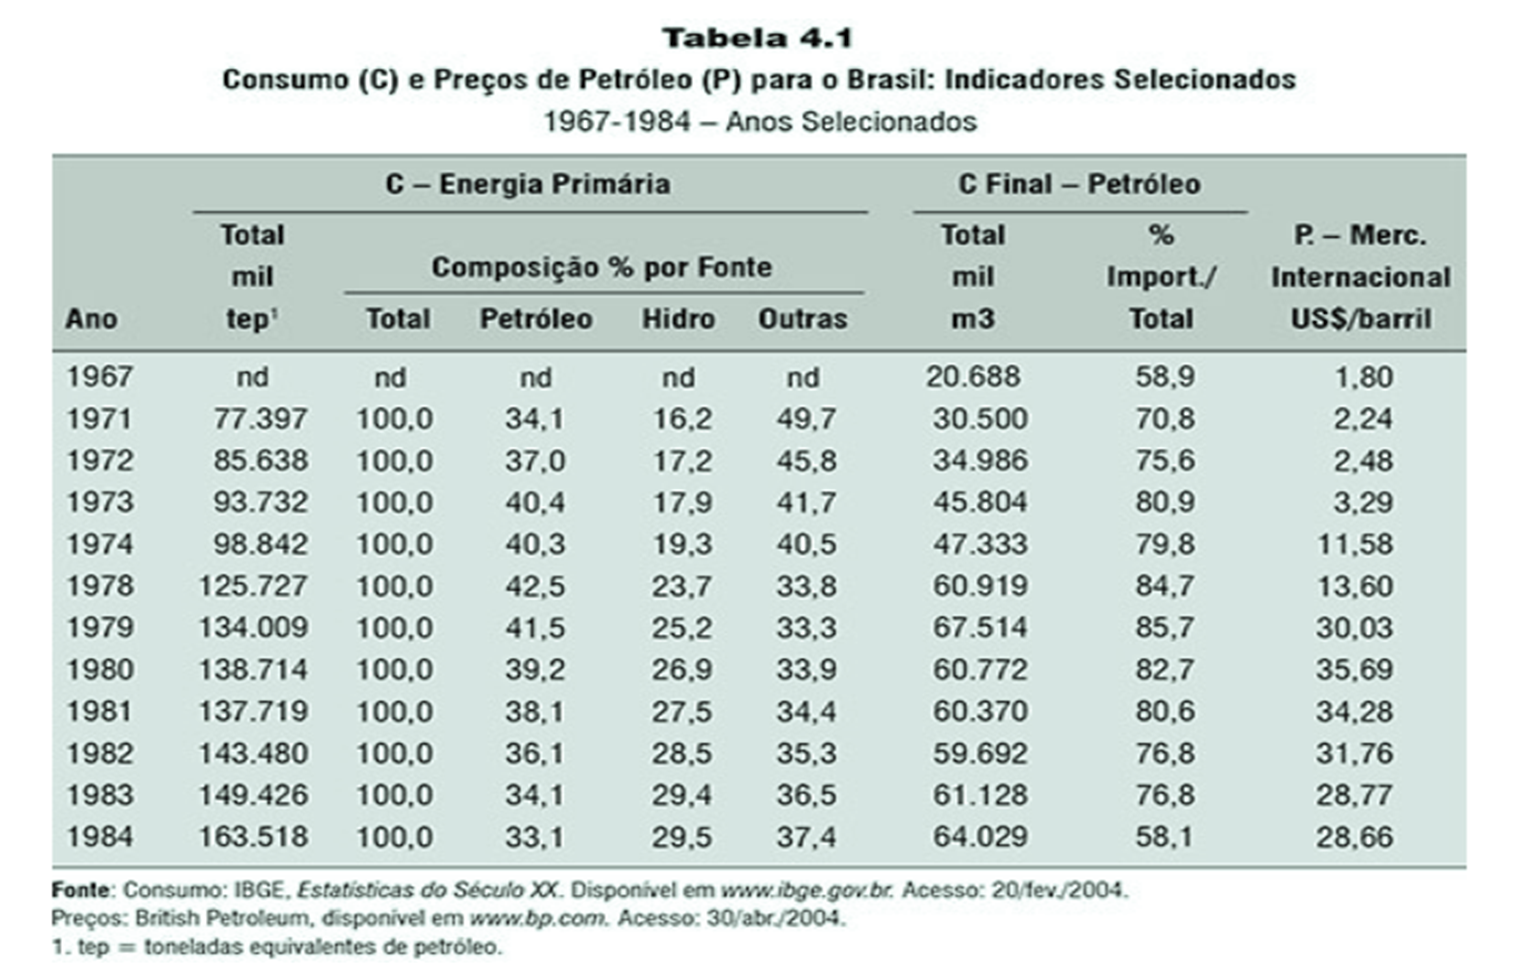
\includegraphics[width=0.7\linewidth]{Imagens/a6i1.png}
\end{figure}
Petróleo é importante para o Brasil dessa época, só de energia primária 37\%, o Brasil importa cerca de 75\% para usar localmente no primeiro choque. Ele saí de cerca de 2 dólares e vai para quase 12 dólares(um aumento de praticamente 6 vezes), lembrando que o Brasil nessa época importava muito petróleo.


\subsection{\textbf{Contexto internacional}}
Demanda agregada e inflação pressionadas\begin{itemize}
    \item há uma demanda mundial aquecida com os aumentos dos gastos militares americanos (Guerra do Vietnã);
    \item demanda mundial por aumentos salariais;
    \item efeitos da queda do dólar em 1971;
    \item expansão do crédito internacional com o mercado de Euromoedas;
    \item A OPEP demostrando organização movimenta os preços (aumento de 4x ao final de 1973).
\end{itemize}

\subsection{\textbf{Choque do Petróleo em 1973}}
Em dezembro de 1973 ocorre o 1º choque do petróleo:\begin{itemize}
    \item de US\$ 3,29/barril (1973) o preço vai para 11,58 em 1974; 
    \item o setor externo brasileiro que estava sob base frágil até 1973, torna-se restritivo em 1974, perdendo a capacidade de importar, consequentemente de crescer.
\end{itemize}

Como o mundo reage ao choque? (1974/75)\begin{itemize}
    \item elevação de juros (reduz atividade econômica e o comércio mundial); 
    \item o que gera piora dos termos de troca;
    \item por outro lado, há presença dos “petrodólares”. O que é isso?
    \item OPEP busca aplicações financeiras para seus superávits, primeiramente nos países industrializados e na sequência nos países em desenvolvimento que concedem mais retorno.
\end{itemize}

\subsection{\textbf{Opções diante do 1º choque do petróleo}}
Três possibilidades são consideradas:\begin{enumerate}
    \item aceitar a restrição externa e ajustar as possibilidades novas de crescimento;
    \item desvalorizar o câmbio, fazendo as exportações crescerem e reduzir a demanda interna por importações (limita o crescimento);
    \item superar a restrição, aumentando a capacidade produtiva para atender o maior consumo de importações e de petróleo, o que também reduziria a necessidade de financiamento externo.
\end{enumerate}

Situação bem delicada a do Brasil e do Geisel durante seu governo(pressões políticas e econômicas extremamente apertadas) nessa época, uma situação com preços altos e seus custos de realizações tão altos quanto.

1º e 2º fatalmente seriam recessivos e 2º traria sério risco inflacionário. 3º seria estrutural e complementaria a \textbf{PSI}(Política de Substituição de Importações; algo já feito no Brasil). O discurso seria: o Brasil transformar-se-ia em uma potência econômica!

A opção escolhida foi (II PND) uma agenda de longo já usada no Brasil. Pois:\begin{itemize}
    \item havia disponibilidade de capital estrangeiro e uma forte pressão política para evitar um ajuste recessivo \textbf{[sobrevida aos militares]}
\end{itemize}

\subsection{\textbf{Política econômica no governo Geisel}}
Mantido Veloso no Planejamento e entrada de Mário Henrique Simonsen(ortodoxo econômico) para realizar a agenda de curto prazo do plano do Geisel(Fazenda; já que Geisel e Delfin Netto brigaram). 

Síntese:\begin{itemize}
    \item Curto prazo – medidas ortodoxas para frear o processo inflacionário (mas sempre modestas, dado o receio da desaceleração econômica)
    \item Longo prazo – investimentos para substituir importações de insumos industriais (II PND)
\end{itemize}

\subsection{\textbf{Medidas}}
O aumento das importações concretiza-se e há piora da balança comercial(já com as consequências do 1º choque do petróleo)\begin{itemize}
    \item executa política monetária restritiva, mas com “cuidado”(lembrando que ele é ministro do Geisel);
    \item medidas para conter as importações, especialmente os produtos desnecessários/supérfluos; 
    \item mantida a política de minidesvalorizações para proteger os exportadores (preocupações com as EX)
    \item são observadas várias circulares e resoluções do Bacen, buscando acelerar a entrada de capitais (empréstimos externos): redução de IR, isenção de IOF para ter oportunidades mais favoráveis para os investidores estrangeiros
\end{itemize}

Há retirada do controle de preços \begin{itemize}
    \item fim da política de congelamento de preços imposta por Delfin Netto, lembrando que isso é uma prática da ortodoxia, a forma como Simonsen conduz suas medidas
    \item trouxe elevação imediata da “inflação oficial”; 
    \item oficializada uma fórmula de correção monetária para dar maior clareza às regras de indexação; Correção monetária(índice que indica o valor do reajusta da inflação monetária) foi um dos nomes dados para o que a ORTN fazia, que era a manutenção do rendimento real ser verificado da forma correta. Simonsen vai registrar formalmente como esse reajuste vai ser feito, qual índice, qual período, acabando com a subjetividade.
    \item determina em lei que a correção monetária viria da variação da ORTN; (antes era de decisões arbitrárias da Fazenda);
    \item Mas, no curto prazo, elevou a incerteza, já que as regras foram mudadas tão repentinamente.
    \item Governo tenta controlar a liquidez;
\end{itemize}

Mas, 1974 marca um ano de grande expansão monetária de 33\% (empréstimos do BB ao setor privado e repasses do Bacen para fundos e programas). 

Também houve elevação da liquidez aos bancos, uma ajuda do Bacen para reduzir efeitos da quebra do Banco Halles (4º maior banco brasileiro).

A política salarial foi alterada: \begin{itemize}
    \item além de mantida a recomposição salarial pelo último ano, caso uma perda futura de inflação fosse verificada, seria recomposta ao salário;
    \item a ideia era pôr fim ao arrocho salarial, considerado como a grande causa da piora da distribuição da renda;
    \item essa piora era uma grande crítica à política econômica dos presidentes militares.
\end{itemize}

\subsection{\textbf{Salário mínimo real, Brasil (1950-1980)}}
\begin{figure}[H]
    \centering
    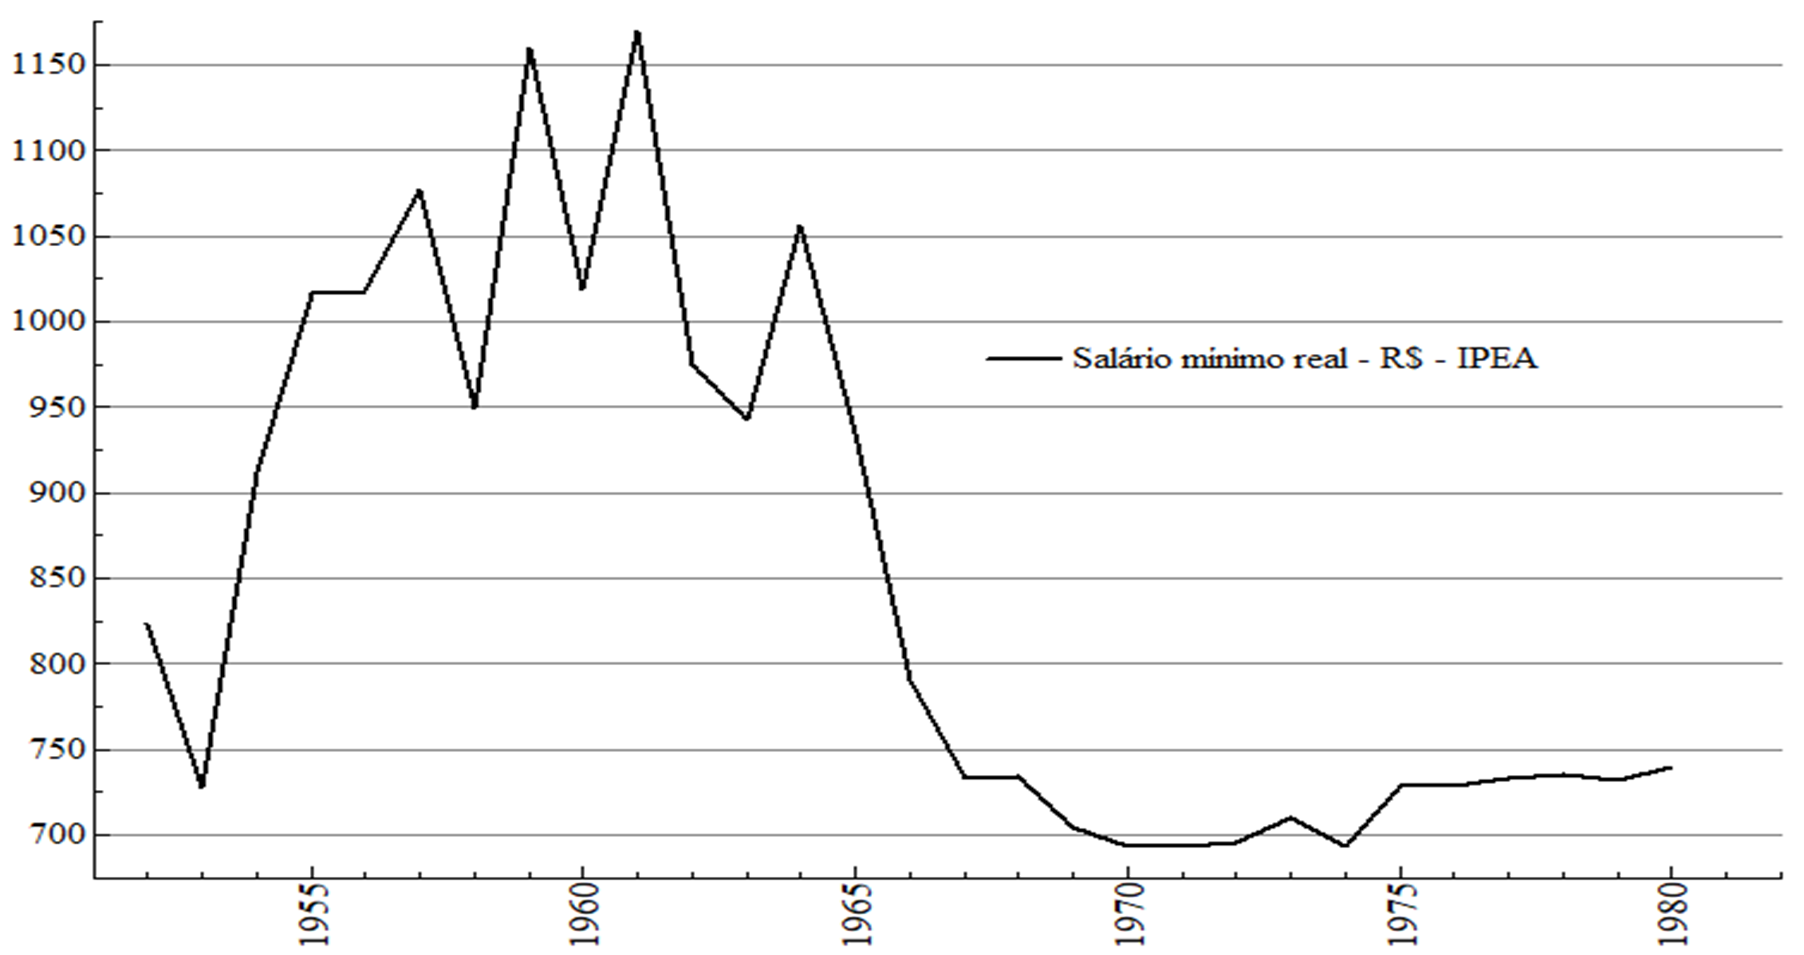
\includegraphics[width=0.7\linewidth]{Imagens/a6i3.png}
\end{figure}

\subsection{\textbf{O fim do breve ajuste recessivo}}
A crise financeira decorrente das incertezas quanto ao futuro da economia era significativa. 

O governo tinha dificuldades políticas crescentes com o crescimento político da oposição da UDN. 

Dessa forma, entre a estabilização e o crescimento:\begin{itemize}
    \item a escolha foi dar prioridade total à continuidade do crescimento.
\end{itemize}

\subsection{\textbf{II PND}}
\textbf{Obs.}: I PND (1971, Médici) - manter o Brasil entre as 10 economias mais fortes do mundo, levando para 8o lugar

Objetivo: promover um ajuste na estrutura de oferta de longo prazo, mantendo o crescimento econômico aliado ao endividamento externo\begin{itemize}
    \item no longo prazo, a necessidade de importações seria menor e a capacidade de exportar do país seria fortalecida.
\end{itemize}

Principais pontos de estrangulamento:\begin{itemize}
    \item Infraestrutura: ampliação da malha ferroviária, rede de comunicações, infraestrutura para produção e comercialização agrícola (ampliação para o mercado interno e exportação).
    \item Bens de capital e insumos: aumentar a produção de aço de 7 para 8 milhões de ton.; triplicar a produção de alumínio; aumentar a produção de zinco de 15 mil ton. para 100 mil. Projeto Carajás (minério de ferro);
\end{itemize}

Setor energético: exploração e produção de petróleo e derivados, ampliação da energia hidroelétrica (Projeto Itaipu); energia nuclear (NUCLEBRAS); energia alternativa aos derivados do petróleo – álcool e combustível.

Instrumentos: \begin{itemize}
    \item crédito do IPI sobre compra de equipamentos; 
    \item depreciação acelerada para equipamentos nacionais; 
    \item crédito subsidiado e formas de reservas de mercado para novos empreendimentos.
\end{itemize}

A política industrial foi sujeita a diversas críticas na medida em que não visualizava que havia certo excesso de oferta na produção nacional frente ao novo ciclo econômico (desdobramentos do 1º choque do petróleo)\begin{itemize}
    \item tanto setor público quanto privado seguiram a lógica de forte demanda por financiamento e autorizações para novos empreendimentos.
\end{itemize}
    
“Ilusão” de continuidade do ciclo anterior no início dos 70. \begin{itemize}
    \item setores privado e público pareciam “mal acostumados” ao padrão de crescer e demandaram fortemente pela sua continuidade. 
    \item o setor privado “parecia saber o que viria pela frente” e tratou de se aproveitar de toda e qualquer vantagem dada para se posicionar no mercado, tendo ganhos e vantagens extraordinários, sem qualquer contrapartida.
\end{itemize}

\textbf{DISCUSSÃO}: deveria ter sido lançado no contexto de Crise do Petróleo? o que deu errado? Deu errado? Quais foram os prós e contras?

De forma geral, parece que o II PND apresentou resultados favoráveis frente aos seus objetivos. \begin{itemize}
    \item houve redução da necessidade das importações de insumos industriais básicos (papel e celulose, fertilizantes, produtos petroquímicos e aço). 
    \item as despesas com esses itens ficaram constantes em termos nominais e as exportações destes aumentaram.
    \item destaque como ponto importante a continuidade no incentivo às exportações (diferenciando-se de experiências anteriores e de outros países). As proporções das EX e das IM no PIB sobem e caem, respectivamente, mesmo diante do 2º choque do petróleo.
\end{itemize}

O plano esteve apoiado em diversos incentivos e estímulos fiscais, cambiais e creditícios. \begin{itemize}
    \item deixou a posição financeira pública brasileira comprometida com elevação do endividamento e queda da carga tributária líquida.
    \item Isso deixaria os instrumentos de ação do governo enfraquecidos na década de 80.
\end{itemize}

Assim o sucesso do II PND, deixou custos: quebra do estado brasileiro. \begin{itemize}
    \item as isenções e endividamento trouxeram comprometimento da receita pública bem como no abastecimento da aceleração inflacionária que seria verificada na década.
\end{itemize}
\newpage

\section{\textbf{Política econômica e problemas econômicos no governo Figueiredo, 1979-1984}}
\subsection{\textbf{Introdução}}
Temas:\begin{enumerate}
    \item O 2º choque do petróleo e o processo de ajuste brasileiro
    \item A recessão da economia brasileira que se inicia em 1981
    \item O grande saldo da BC em 1984
\end{enumerate}

\textbf{O que é importante?}:Identificar a opção de ajuste diante da piora do endividamento externo e avaliar quais foram os desdobramentos até o reequilíbrio externo

\textbf{Leitura}: Economia Brasileira Contemporânea, (Cap. 4, trecho do governo Figueiredo) 

\subsection{\textbf{Transição Geisel - Figueiredo}}
A dívida externa crescente e a disputa entre os militares reduzia a viabilidade política de uma prática anti-inflacionária mais séria\begin{itemize}
    \item insistência se dá pelo método gradualista;
    \item foco passa a ser no setor externo: gerar acúmulo de reservas. 
\end{itemize}

Ao assumir em 79, Figueiredo, transfere M. H. Simonsen para o Planejamento (Seplan)\begin{itemize}
    \item o Seplan presidia o Conselho Monetário Nacional, supervisionava a Secretaria de Receita Federal e o Conselho interministerial de preços;
    \item em tese, isso permitiria maior controle da política econômica, tornando-a mais coesa e coerente.
\end{itemize}

\subsection{\textbf{Política econômica no governo Figueiredo}}
Início da gestão Simonsen (contracionista antes mesmo do 2º choque)\begin{itemize}
    \item controlar expansão de meios de pagamento e de crédito bancário (inclusive do BNDE);
    \item conter as despesas (subsídios e os investimentos das estatais);
    \item nova política cambial: promover desvalorizações reais da taxa de câmbio.
\end{itemize}

Mas essa política elevaria a incerteza cambial dos devedores em dólares.

Como o governo amenizou essa incerteza? 

\subsection{\textbf{Nova política cambial}}
Resoluções 432 e 230 do Bacen:\begin{itemize}
    \item permitem empresas e bancos depositarem no Bacen os compromissos devidos antes do vencimento das obrigações; 
    \item Bacen seria na prática o responsável por liquidar as dívidas;
    \item ocorre que isso transfere risco cambial  e custos de desvalorizações futuras para o governo!
\end{itemize}

Mas o que isso significa?\begin{itemize}
    \item interfere na dívida pública (despesa pública financeira);
    \item desvalorizações cambiais elevam essas despesas;
    \item desvalorizações agravam a crise fiscal brasileira!
\end{itemize}

\subsection{\textbf{O 2º Choque do petróleo muda o contexto internacional}}
O 2º choque do petróleo muda o contexto (meados de 1979) 

Simonsen: ajuste recessivo é a única forma de reequilibrar o BP!\begin{itemize}
    \item seu posicionamento forte e medidas contracionistas geram forte oposição no governo e no setor privado;
    \item especialmente de Delfim Netto que estava na agricultura;
    \item Simonsen renuncia em agosto de 1979;
    \item Delfim retorna ao comando da política econômica
\end{itemize}

\subsection{\textbf{Petróleo e a economia brasileira (1967-1984)}}
\begin{figure}[H]
    \centering
    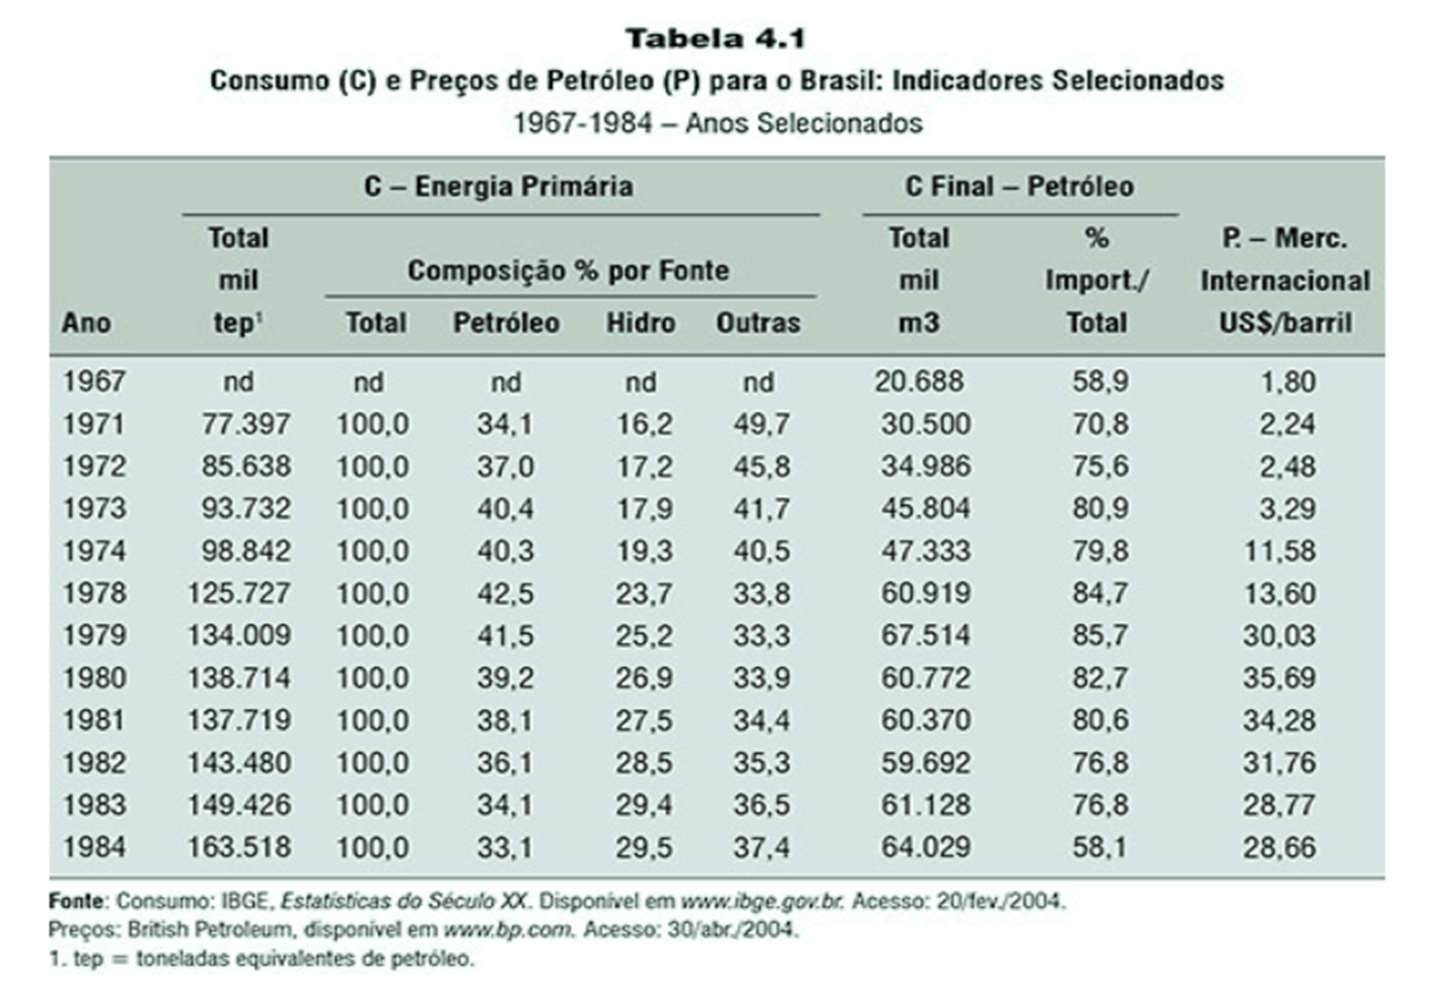
\includegraphics[width=0.7\linewidth]{Imagens/a8i1.png}
\end{figure}

\subsection{\textbf{Contexto e efeitos importantes}}

\begin{itemize}
    \item Brasil com elevado endividamento externo e ainda dependente das IM de petróleo
    \item Ocorre o 2º choque do Petróleo (1979)
    \item O FED eleva fortemente as taxas de juros (1979-82)
\end{itemize}

Quais seriam os efeitos esperados para a economia brasileira?\begin{itemize}
    \item Pioram os déficits em conta corrente;
    \item Há maior pressão inflacionária;
    \item Compromete arrecadação do governo e posição financeira das estatais.
\end{itemize}

Assim:\begin{itemize}
    \item O contexto internacional e a opção de ajuste adotada direcionam as fases econômicas do governo Figueiredo
    \item É o período da ``crise da dívida externa''. Começa a ``década perdida''!
\end{itemize}

\begin{figure}[H]
    \centering
    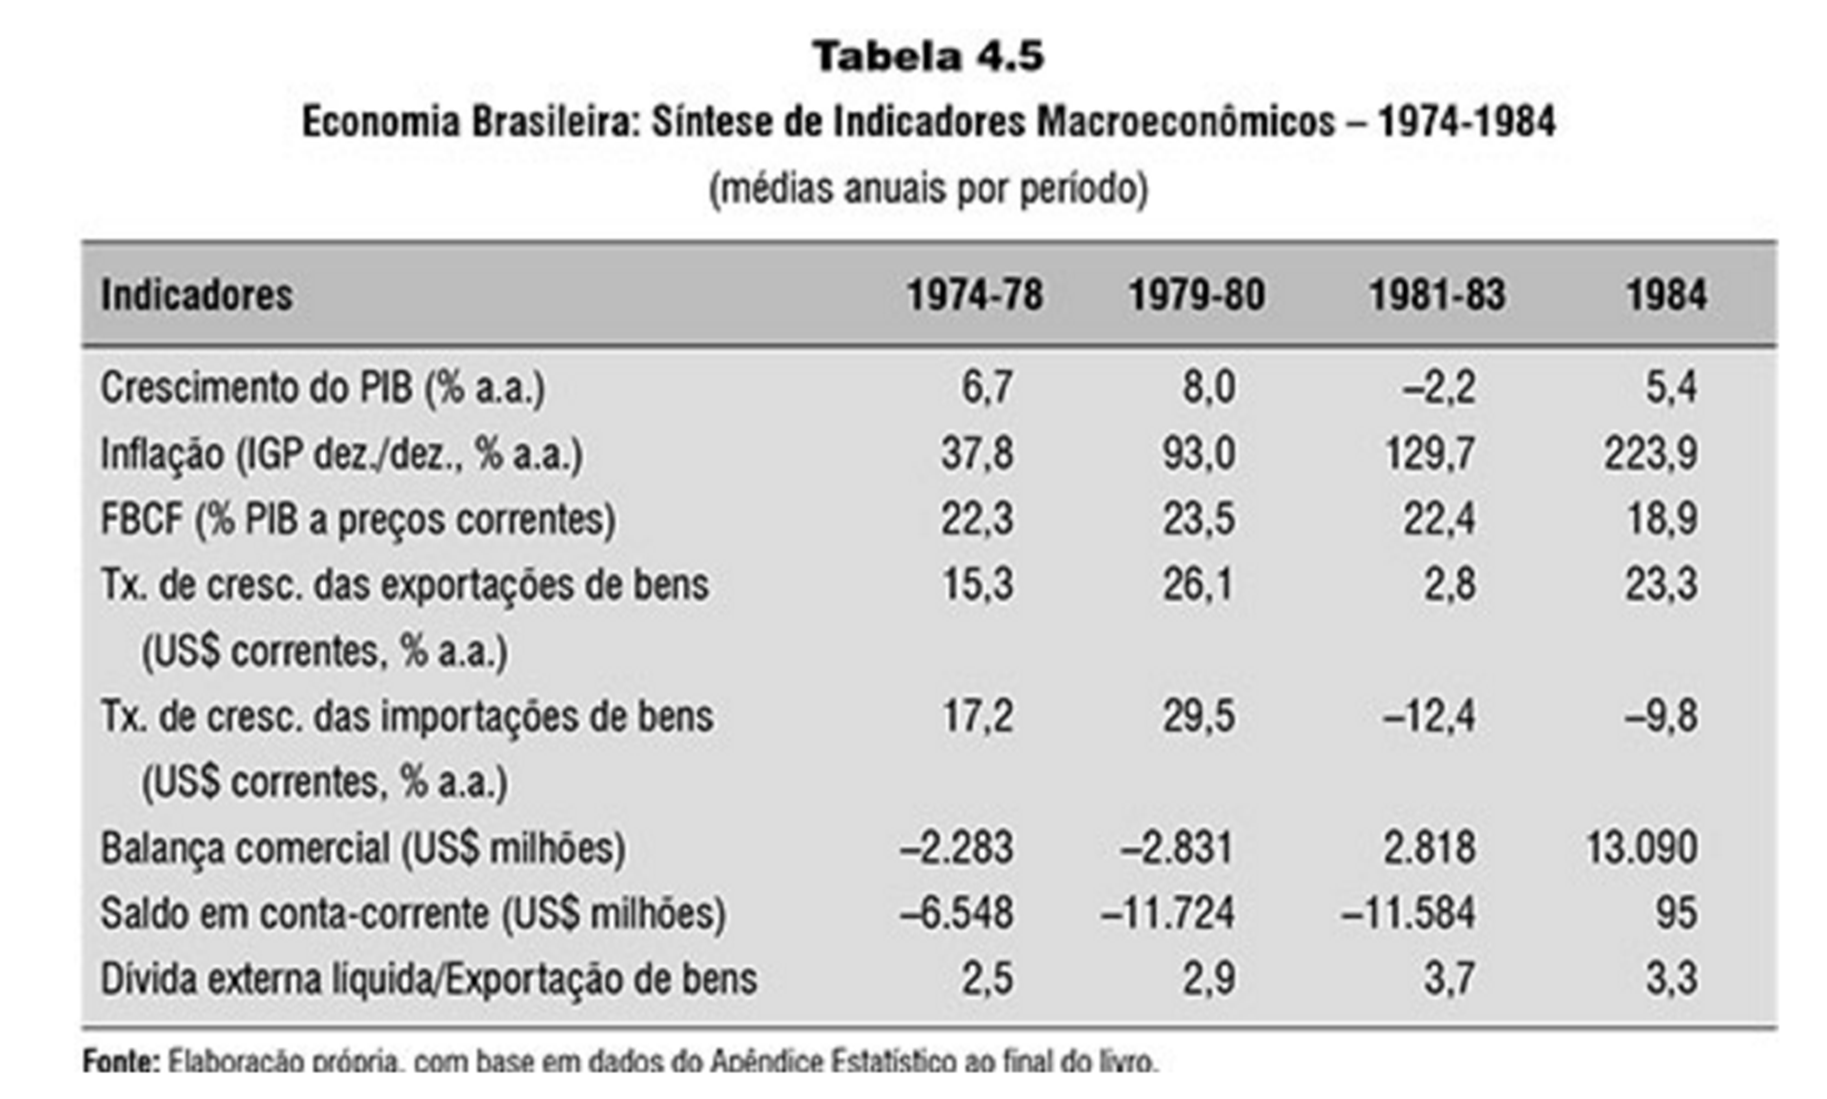
\includegraphics[width=0.7\linewidth]{Imagens/a8i2.png}
\end{figure}

\subsection{\textbf{Diagnóstico de Delfim}}

\begin{itemize}
    \item Crise do setor externo tinha causa principal no desajuste de preços relativos que distorcia a demanda entre os diversos setores;
    \item A causa não era um ``simples'' excesso generalizado de demanda;
    \item Produção doméstica e exportações devem ser estimuladas!
\end{itemize}

\textbf{Ações e instrumentos de política econômica}\begin{itemize}
    \item Controle monetário e de crédito foram reforçados;
    \item Maxidesvalorização cambial (30\%) em dezembro de 1979;
    \item Tarifas públicas são corrigidas e gastos do governo controlados;
    \item Déficit público deveria ser controlado, pois alimentava a inflação.
\end{itemize}

\subsection{\textbf{Ações e instrumentos de política econômica}}

Mas subsídios cresceram no período (para agricultura e exportação);

Há mudança no regime de reajuste salarial (reajustados semestralmente nos setores públicos e privados).


\textbf{Também houve medidas heterodoxas:}\begin{itemize}
    \item Há controle de juros, maior indexação de salários e desvalorização cambial;
    \item Prefixação da correção monetária (em níveis inferiores aos da inflação) para tentar efetuar controle das expectativas inflacionárias durante parte do ano de 1980;
    \item Banqueiros estrangeiros não avalizam tal experimento e há redução das reservas internacionais.
\end{itemize}

\subsection{\textbf{Resultados das medidas de Delfim}}

As correções cambiais, dos preços públicos e mudança do reajuste salarial aceleraram a inflação;

A recessão foi evitada, dado o aumento das exportações e do crescimento ``inercial'' a partir dos investimentos do II PND;

Desequilíbrio externo não foi resolvido.\begin{itemize}
    \item Maxidesvalorização de 1979 não funcionou, pois houve forte elevação inflacionária;
    \item Exportações aumentaram, mas déficit comercial cresceu (forte aumento dos preços do petróleo e do quantum das IM em 1979);
    \item Elevação dos juros americanos aumentaram os compromissos externos.
\end{itemize}

\subsection{\textbf{Política econômica no governo Figueiredo}}

Superávits na conta capital não cobriram a conta corrente negativa;

Há forte perda de reservas internacionais.

\textbf{O insucesso do ajuste de 79 e a piora do setor externo fez o governo assumir a necessidade de um ajuste explicitamente recessivo}\begin{itemize}
    \item Redução da absorção interna foi a prática nesse período, atraindo foco para as exportações e reduzindo as importações;
    \item A aposta não foi pela desvalorização dada a falta de credibilidade após as medidas de 79 e a recessão mundial que não absorveria(não havia compradores) mais exportações.
\end{itemize}

Base do ajuste contracionista\begin{itemize}
    \item Contenção salarial e controle de gastos
    \item Elevação das taxas de juros e contração da liquidez real (reduz consumo e incentiva agentes a buscar juros menores no exterior)
    \item permanece com estímulos às exportações
    \item elevação da carga tributária

\end{itemize}

\subsection{\textbf{Resultados da política contracionista}}
Efeito quase nulo na inflação\begin{itemize}
    \item mostra rigidez inflacionária, apoiando a tese inercial. 
\end{itemize}

Forte recessão a partir do início de 1981, formando um cenário de estagflação

Há reversão significativa da balança comercial em 1981  \begin{itemize}
    \item recessão + efeitos estruturais do II PND 
\end{itemize}

\subsection{\textbf{Recessão segue em 1982}}

A recessão mundial é mais profunda:
\begin{itemize}
    \item Brasil não consegue mais uma BC significativamente positiva, com a queda das exportações;
    \item queda das importações foi forte, mas o compromisso externo dada a subida dos juros que gerava o déficit em conta corrente independia do tamanho da redução da absorção;
    \item contexto torna-se mais grave, quando em agosto de 1982, o México decreta a moratória;
    \item isso impulsiona o contato brasileiro com o FMI e com bancos privados estrangeiros, mas a negociação não traz os desejados recursos financeiros.
\end{itemize}

Internamente:
\begin{itemize}
    \item para o discurso governista não há necessidade de se recorrer ao FMI.
\end{itemize}

\subsection{\textbf{O fundo do poço (1983)}}

O ano foi o início de um período marcado por uma série de cartas enviadas ao FMI:
\begin{itemize}
    \item O elevado grau da indexação da economia brasileira e da participação do setor público complicou os termos do acordo.
\end{itemize}

O governo promove:
\begin{itemize}
    \item Maxidesvalorização em 83 de 30\% e novos programas de incentivos de crédito para as exportações;
    \item Desindexação parcial dos salários, eliminando o adicional de 10\% sobre o INPC semestral, reduziu percentuais de correção para faixas até 15 salários e eliminou a livre negociação para maiores de 20 salários;
    \item Na prática, gera queda de 15\% do poder de compra dos salários ao longo de 1983.
\end{itemize}
    
Uma sequência de fatores gera o reequilíbrio externo em 1983:
\begin{itemize}
    \item Recessão interna, desindexação salarial, melhoria americana e desvalorização cambial.
\end{itemize}

Mas a inflação estava descontrolada e agravada por dois choques:
\begin{itemize}
    \item \textbf{Agrícola}: parte do choque agrícola veio do esforço exportador e consequente desabastecimento interno;
    \item \textbf{Cambial}: a maxidesvalorização aumentou os custos dos insumos importados.
\end{itemize}

\subsection{\textbf{O ajuste completo e o fim da recessão, 1984}}

\textbf{PIB real cresceu 5,4\% em 1984. Como explicamos?}

\begin{itemize}
    \item O salário apresentou recuperação;
    \item Consumo antecipado frente à piora das expectativas inflacionárias promoveram aceleração do consumo, levando vários setores industriais a um forte crescimento;
    \item Há relaxamento da restrição externa em 1984, graças às importações americanas;
    \item Dado o aumento dos preços agrícolas, a renda rural aumenta, gerando aumento da compra de bens intermediários e maquinaria industrial;
    \item A indústria extrativa mineral sobe 30,5\%, uma expressão do aumento da produção nacional de petróleo, permitindo forte redução das despesas com este item.
\end{itemize}

O ajustamento permitiu, além de pagar os juros da dívida (40\% das EX), como também equilibrar a conta corrente.

\begin{itemize}
    \item Foi um ajuste com crescimento do PIB e saldo comercial elevado. Isso mudou o padrão de negociação junto ao fundo;
    \item Mas o não cumprimento das necessidades nominais de financiamento e o déficit operacional do setor público postergaram negociações para 1985 sob novo governo (iriam se mostrar bem difíceis).
\end{itemize}

\subsection{\textbf{O BP ajustado em 1984}}

Depois de forte desequilíbrio, o BP estava melhor no final de 1984.

\textbf{Fatores importantes do ajustamento externo}:
\begin{itemize}
    \item A demanda por exportações foi importante para um ajustamento externo não recessivo;
    \item De fato, a aposta de Geisel tinha sido “perigosa”.
\end{itemize}

\textbf{Como podemos retomar os resultados do II PND diante desse ajuste?}
\begin{itemize}
    \item A estratégia de longo prazo (IIPND) parece ter gerado bons dividendos com forte queda do coeficiente de importação (IM/PIB) e aumento do coeficiente de exportação (EX/PIB).
\end{itemize}

\begin{figure}[H]
    \centering
    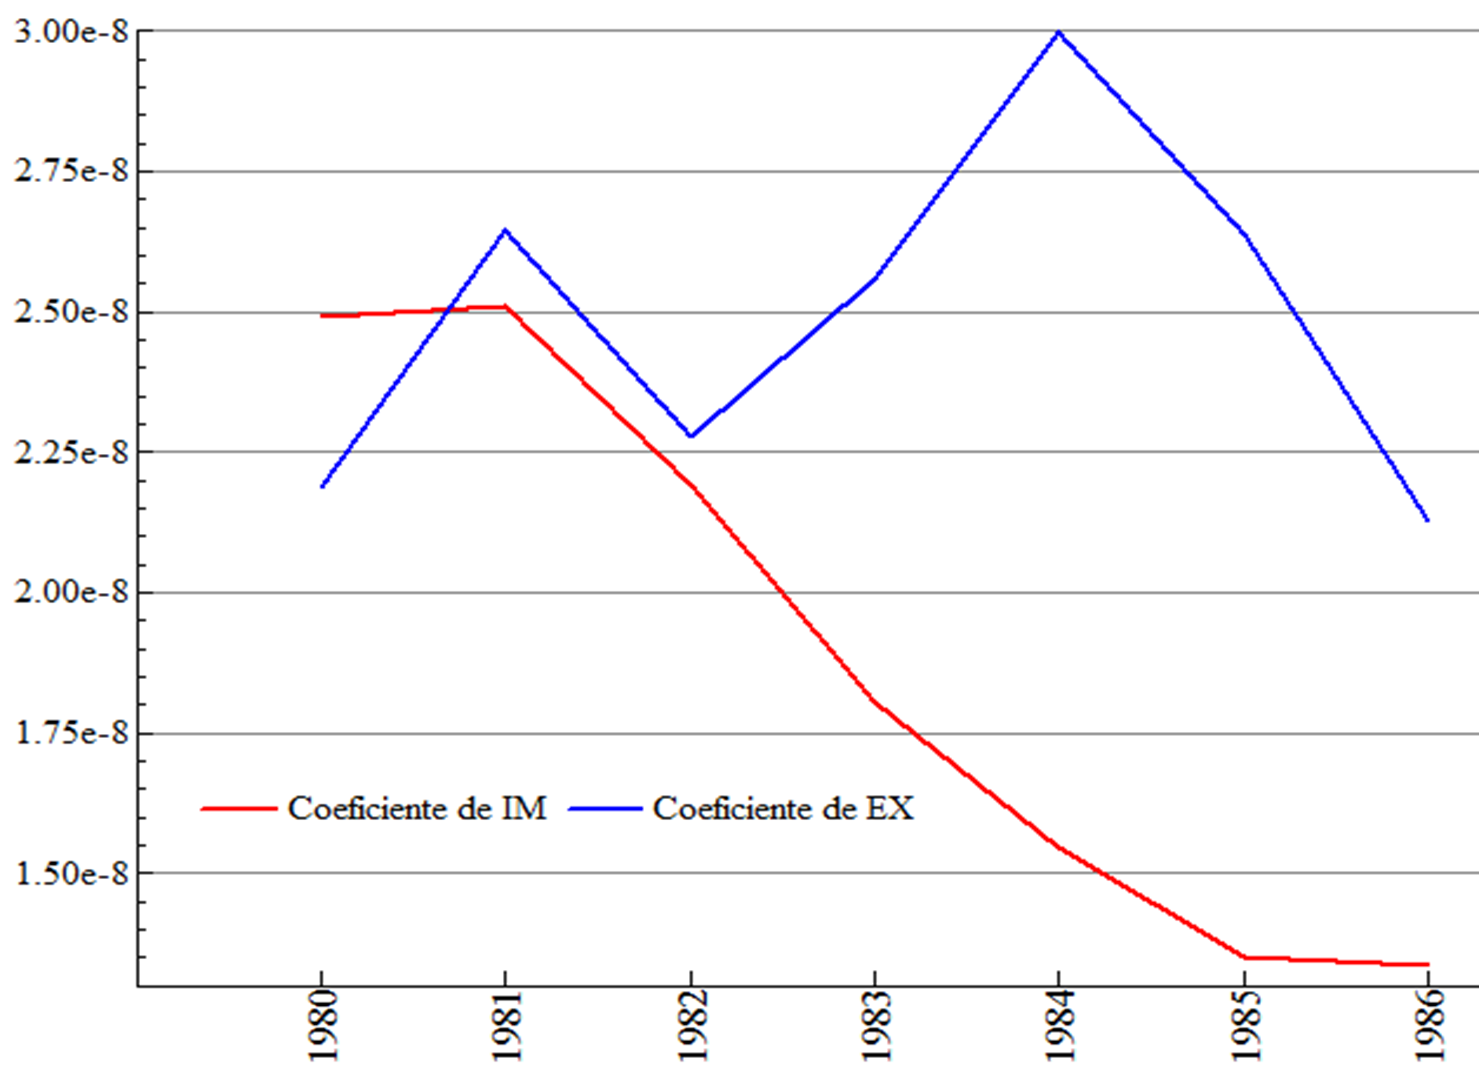
\includegraphics[width=0.7\linewidth]{Imagens/a9i1.png}
\end{figure}

\subsection{\textbf{Ainda os resultados do II PND}}

Mas a opção pelo financiamento externo gerou efeitos negativos severos:
\begin{itemize}
    \item O governo parecia considerar condições “eternas” de juros baixos e capital externo abundante;
    \item Não se deu a devida importância de como uma recessão internacional pode derrubar as exportações;
    \item E o contexto externo mudou! (choque do petróleo e de juros);
    \item Houve deterioração da inflação e da dívida pública;
    \item A inflação não respondia mais às alterações de demanda;
    \item Nenhuma atenção foi dirigida à questão da indexação.
\end{itemize}

\subsection{\textbf{A crise fiscal do estado brasileiro}}

\textbf{Por que a dinâmica de crescimento da dívida pública piora?}
\begin{itemize}
    \item Não se cogitou uma reforma fiscal para buscar um reordenamento do setor público brasileiro;
    \item A dívida pública crescia mesmo sob política fiscal contracionista. Por quê?
    \begin{itemize}
        \item Correção monetária e as resoluções 432 e 230 do Bacen;
        \item Há descontrole inflacionário e duas maxidesvalorizações!;
        \item Despesas financeiras aumentam ao contabilizarem custos com inflação e custos cambiais.
    \end{itemize}
\end{itemize}

Assim, o Brasil vive forte crise fiscal no início da década de 80.

\newpage
\section{\textbf{As tentativas de estabilização : Introdução}}

O Brasil usou do que o mundo ofereceu e o Brasil pagou o que mundo exigiu.

\subsection{\textbf{Introdução}}
\textbf{Temas}\begin{enumerate}
    \item \textbf{Entender a formação do processo inflacionário brasileiro}
    \item \textbf{Entender o processo e suas consequências}
    \item \textbf{Indexação e propostas de desindexação}
\end{enumerate}

\textbf{O que é importante?}

Identificar a lógica do processo inflacionário, quais as dificuldades no seu combate e as propostas para desinflacionar a economia brasileira.

\textit{Leitura: Ordem do Progresso (cap. 14) e Economia Brasileira Contemporânea (cap. 5)}

\subsection{\textbf{Contexto Político}}

Período com ``esperanças renovadas''(as coisa milagrasoamente vai se resolver); haveria retorno das liberdades, fim da inflação, crescimento e redistribuição de renda;

Ocorre a transição ``democrática'' via eleições indiretas(a sociedade pedia eleições diretas; mas o congresso decidiu que ia ser indiretamente), da qual o 1º Presidente (Tancredo Neves(conservador e alinhada com o centro)) morreu(antes de assumir), assumindo José Sarney(vice de Tancredo; Sarney era mais alinhado com os governos anteriores);

Sarney implementou ao longo de seu governo 3 planos de estabilização; Todos fracassaram!

Além disso , tivemos nesse meio tempo, tivemos a questão da famosa \textbf{constituição de 88}.

\subsection{\textbf{Perspectiva histórica da formação do processo inflacionário do Brasil}}

Como que as medidas tomadas no Brasil com a intenção de crescimento gerou esse ''monstro'' descontrolado chamado de hiper-inflação.  

\textbf{Fonte:} PASTORE, A. C.; PINOTTI, M. C. O \textit{Paeg} e as políticas econômicas dos anos 1960 e 1970. In: MOURA, A. R. (Org.). \textit{Paeg e Real dois planos que mudaram a economia brasileira}. Rio de Janeiro: FGV, 2007. p. 19 - 79.

\textbf{Principais pontos:}\begin{itemize}
    \item O \textbf{Paeg} (1964) optou pela indexação, ou seja, possibilitou a ação de forças propagadoras da inflação; (seria possível conviver com inflação?);
    \item O Bacen nasceu fraco no PAEG(perspectiva anacrônica, pois olhamos com os conhecimentos macros de políticas monetárias atuais) , sem compromisso com a estabilidade de preços e o BB ainda era o banco do governo(formação institucional fraca);
    \item Delfim (1968) utilizou política monetária expansionista para estimular o crescimento econômico(medidas fiscais expansionistas) e fez controle de preços da economia; 
    \item Ocorreu uma ampliação da indexação salarial(em relação a inflação passada) ao longo do tempo e adesão ao regime de minidesvalorizações baseadas na PPC(contaminando diversos preços com a inflação passada);
    \item Utilizou fortemente o endividamento externo para financiar o II PND, o que deteriorou fortemente a estrutura fiscal brasileira, isso corrompe a estrutura inflacionária.
\end{itemize}

Esses fatores(e diversos outros, como choques do petróleo, crise de dívida externa) atuaram ao longo do tempo conjuntamente e foram observados diversos choques: o que foi gerado?

Ao ano, o índice de inflação chegava a quase 5000\% ao ano. Ao mês podia chegar 90\%. Os processos de desinflação promulgados, geravam mais inflação. Ao ponto que o Plano Cruzado acelerou a inflação a níveis que não foram atingidos anteriormente. O problema não era reduzir a inflação, o problema era que os planos eram insustentáveis e fracassavam em manter a inflação baixa.

\begin{figure}[H]
    \centering
    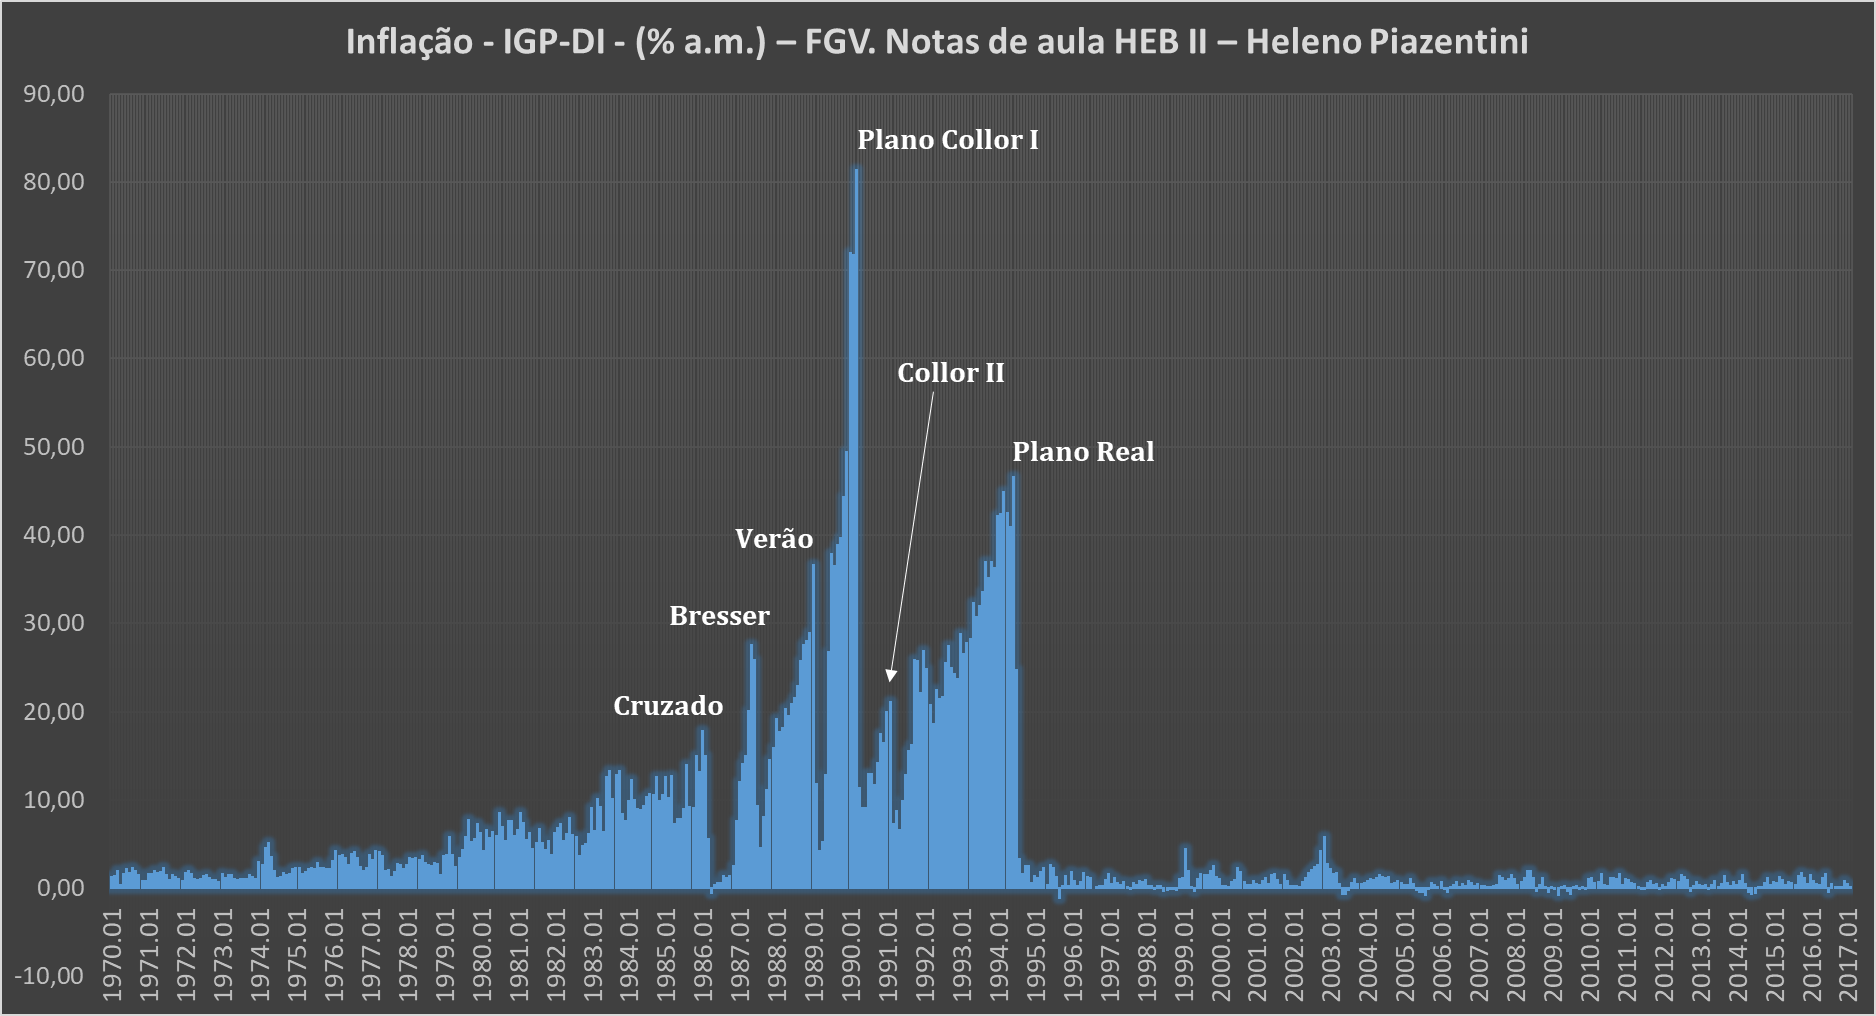
\includegraphics[width=0.7\linewidth]{Imagens/a10i1.png}
\end{figure}

\subsection{\textbf{HPE Brasil}}

Antes um pouco do debate das ideias econômicas(algo não incomum) no Brasil(algo bem intenso em comparação aos outro países). Nos anos 1980, o foco do debate econômico muda:\begin{itemize}
    \item Nas décadas anteriores(JK), o debate era como tornar o Brasil uma ``economia desenvolvida'' (\textbf{estruturalistas(PSI; a mais usada até a chegada dos militares) vs ortodoxos(baixa interferência estadual)});
    \item Agora, o debate é outro, sobre a inflação elevada. Qual a causa principal da inflação brasileira(isso vai definir a forma de pensamento econômico)? Porque ela não cede com as políticas contracionistas (Recessão de três anos)?(\textbf{inercialistas(heterodoxo; isso era algo novo para os economistas dos anos 80) vs ortodoxos});
\end{itemize}

\textbf{Para os inercialistas}(heterodoxos), a economia brasileira está sob indexação(regras de preços atrelados a inflações passadas) generalizada, assim há o ``carregamento'' da inflação passada para o presente (inércia inflacionária).

\subsection{\textbf{O processo de formação de preços em regime de alta inflação (O Brasil dos anos 1980)}}
Como se dá a formação de preços? O que importa para formação de preços? Custos de produção, margens de lucro, planos de negócios, demanda. Isso são coisas triviais. Mas tudo isso que só funciona em economias com inflação controladas e estáveis. 

Em economias que estão em processo de alta inflação, a definição de preços não é regido por esse processo.

\textbf{Conceitos importantes}

\begin{itemize}
    \item Preços relativos: Um cara de que trabalha com a produção de arroz e um outro produz feijão. Cada um olha para o produto que produz para definir seus preços. Mas em alta inflação, não é só isso que se leva em consideração, nessa situação os produtores querem fazer o melhor repasse(a inflação passada integral) para não sair perdendo. Em termos reais, quem repassa menos que a inflação, perde em todas as questões. Eles são direcionadores para os agentes econômicos para se guiarem em relação ao preço final de seu produto (eles olham para o seu e para o dos outros).
    \item Reajustes fora do equilíbrio e dessincronizados: Um apartamento que é alugado ele tem dias, pré-datados, que seu aluguel vai ser ajustado de acordo com a inflação, de maneira controlada e gradativa. Mas em economia de alta inflação esses reajustes são maiores do que o normal, o reajuste pode ser maior que a inflação (por isso fora do equilíbrio), e cada produtor (ou qualquer comerciante, prestador de serviço) está fazendo esses reajustes em períodos diferentes, tendo um descompasso em ajustes, em certo momento um bem foi reajustado pela inflação e outro não, mas em outro momento, o bem que não foi reajustado é reajustado pela inflação e também pelo reajuste do outro. Tudo e todos estão perdendo em termos relativos sempre.  
    \item Conflito distributivo: Resultado desses "Reajustes fora do equilíbrio e dessincronizados", é um resultado de um lugar que está em um processo de "terra sem lei". No mundo de alta-inflação, cada um quer o melhor para si sempre, eles querem ter o melhor repasse de inflação. Todos querem reajustar seus preços acima do equilíbrio, no limite todo dia isso, para não ficar atrás de ninguém. 
    \item Inércia inflacionária: Resultado do "Conflito Distributivo". Gerando o seguinte canal : \(\text{Reajustes fora do equilíbrio e dessincronizados}\rightarrow \text{Conflito distributivo}\rightarrow\text{Inércia Inflacionária}\).
\end{itemize}

Os planos de inflação querem mexer nessas variáveis, eles querem reajustar as forma de fixação de preço, eles querem trazer regras para esse realidade de "Terra sem lei" de reajuste.

\subsection{\textbf{O processo inflacionário}}

\textbf{Problemas para formular um plano de estabilização:}\begin{itemize}
    \item Os agentes sabem que irão perder valor, pois há inflação crescente e desejam se proteger a todo minuto;
    \item Os reajustes dos preços são fechados com valores acima do equilíbrio;
    \item Essa situação de desequilíbrio é reproduzida ao longo do tempo e de modo generalizado por todos;
    \item Os reajustes salariais(contratos, etc) são dessincronizados;
    \item Trabalhadores e contratos estariam sempre em posições diferentes;
    \item A sensação é de que seu preço relativo sempre está ``ganhando''(o pessimista sempre pensa que o outro está ganhando dele);
    \item Neste cenário, o processo de formação de preços está desequilibrado;
\end{itemize}

Ou seja: terminar abruptamente com a inflação causaria grandes redistribuições de rendas. Antes de estabilizar, seria necessário fazer a conversão de todos os preços e contratos pelo seu valor médio, ou seja, seu valor de equilíbrio. Caso contrário, após a estabilização, os agentes continuariam com a sensação de desequilíbrio e a inflação voltaria.

\textbf{Em síntese:} os agentes sempre tentam reduzir seus prejuízos, mas isso não é um processo coordenado entre todos. Mundo sem regras.

Um reajuste de contrato deixa agentes e outros contratos defasados. Os agentes tentando se defender buscam reajustes acima do equilíbrio e o ciclo segue de forma generalizada;

\textbf{Conclusão:} em regime de alta inflação, um plano de estabilização deverá: previamente coordenar todos os agentes de modo a levá-los para um cenário equilibrado de preços relativos.

\subsection{\textbf{Contexto Econômico}}

Crescimento econômico de 5,4\% (1984) e de 7,8\% (1985) do PIB, resultados do Governo Figueiredo e Delfim Netto. Acompanhado de melhora das contas externas. Mas a inflação superou 100\% em 1980 e acelerou a partir da maxidesvalorização de 1983, superando os 220\% em 1984. Recessão de 1981 até 1983 e práticas contracionistas pouco reduziram a aceleração inflacionária..

Consenso era que o PAEG havia introduzido a lógica da correção monetária e ao longo do tempo a indexação se generalizou. Seria necessária a desindexação da economia(agentes pararem de olhar para o passado) e reorganização do processo formador de preços.

A grande discussão: como desindexar a economia?

\subsection{\textbf{O que é indexação?}}

Correção periódica e automática de preços com base na inflação acumulada desde o último reajuste.

\textbf{Qual sua origem?}\begin{itemize}
    \item Introduzida com as reformas de 1965-68, quando títulos financeiros do Tesouro passam a ser corrigidos pela inflação (Obrigações Reajustadas do Tesouro Nacional, \textbf{ORTNs}).
    \item As \textbf{ORTNs} deveriam permitir viabilidade no financiamento de longo prazo da dívida pública;
    \item Tornou-se referência para financiamento de longo prazo (BNH);
    \item Na prática, passou a ser a referência de todos os contratos, o indexador da economia brasileira.
\end{itemize}

\textbf{Implicação da indexação na política econômica?}\begin{itemize}
    \item Torna a política monetária pouco eficaz no combate à inflação.
\end{itemize}

\subsection{\textbf{Propostas de desindexação}}

\begin{enumerate}
    \item \textbf{``Pacto Social''} (economistas do PMDB(Sarney estava aqui) e da Unicamp(Departamento de Economia))
    \begin{itemize}
        \item A inflação no Brasil era resultante de uma disputa entre os setores da sociedade que buscavam maior participação na renda nacional – era o ``conflito distributivo''; Isso é ideia de grupo \textbf{heterodoxo}, já que eles estão falando de inércia.
        \item A solução seria um acordo entre empresários e trabalhadores arbitrado pelo governo. Todos ganhariam com o fim da inflação;
        \item Não aumentar os preços por determinado período de tempo seria o acordo.
    \end{itemize}
    
    \item \textbf{``Choque ortodoxo''} (economistas da FGV-RJ)
    \begin{itemize}
        \item Não havia nada de peculiar na inflação brasileira;
        \item A causa era a expansão monetária excessiva que financiava a expansão de um Estado acima de sua capacidade de arrecadar receitas;
        \item As tentativas no início da década foram incompletas e ineficientes, por isso, não tiveram sucesso;
        \item A receita seria: severos cortes de gastos, aumento de receitas e corte brusco da emissão monetária e de títulos da dívida.
    \end{itemize}

    \item \textbf{``Choque heterodoxo''} (Francisco Lopes da PUC-RJ)

    \item \textbf{``Reforma monetária''}(Proposta Larida) (André Lara Resende e Pérsio Arida da PUC-RJ)
    
    \textbf{Ambas partiam das seguintes evidências:}
    \begin{itemize}
        \item O componente de realimentação pela inflação passada (inércia; autorregressiva) era a \textbf{principal} causa;
        \item Variações do hiato do produto influenciavam pouco a inflação;
        \item O fracasso das políticas do FMI indicavam que a inflação não tinha origem em excesso de demanda;
        \item Não acreditavam na viabilidade de um ``pacto social'';
        \item As propostas eram politicamente atrativas(sem gerar restrição), pois não exigiam práticas restritivas e levariam salários e rendas para seus valores médios.
    \end{itemize}
\end{enumerate}

\textbf{Divergências entre Francisco Lopes e Pérsio Arida/Lara Resende(Apesar de ambas serem heterodoxas):}
\begin{itemize}
    \item Para Francisco Lopes: A solução para a desindexação seria compulsória, via congelamento de preços.
    \item Para Pérsio Arida e Lara Resende:
    \begin{itemize}
        \item O congelamento não permitiria as autocorreções via mercado; os agentes não querem nada de imposição de agentes que estivessem acima.
        \item A proposta seria introduzir uma moeda indexada que circularia paralelamente à moeda brasileira (proposta LARIDA). Para gerar uma conversão para um moeda sem inflação e isso de modo orgânico, e quando o todos adotassem a nova moeda sem inflação, a moeda antiga com inflação iria se extinguir.
    \end{itemize}
    \item Os planos Cruzado, Bresser e Verão seguiram com o congelamento(e fracassaram) e o Plano Real (1994) ``adotou'' a LARIDA(mas com muitas modificações, mas deu certo).
    \item O plano Collor é tão curioso que não se aplica a nenhuma dessas situações.
\end{itemize}

\subsection{\textbf{De volta ao contexto: o ano de 1985}}

Expectativa sobre a Nova República: haveria aumento do salário real e redução da inflação (``pacto social''), mas a política econômica inicia-se com medidas de austeridade fiscal e monetária.\begin{itemize}
    \item A estratégia gradualista falha.
\end{itemize}

O embate cresceu entre Dorneles, visão ortodoxa, e Sayad do Planejamento (heterodoxo).\begin{itemize}
    \item Dorneles foi substituído por Dilson Funaro para buscar a estabilidade da inflação;
    \item Diante das falhas dos ajustes recessivos, Sarney escolheu a proposta do ``Choque heterodoxo'' de Francisco Lopes.
\end{itemize}

\newpage
\section{\textbf{As tentativas de estabilização(Planos Bresser e Verão)}}
\subsection{\textbf{Retomando o Plano Cruzado}}
\textbf{Plano Cruzado}: anúncio do presidente José Sarney, em 27 de fevereiro de 1986 (\href{https://www.youtube.com/watch?v=TOdzFViggrU}{link para vídeo}).

Lógica do Plano a partir do diagnóstico da inflação inercial\begin{itemize}
    \item Reorganizar o processo de formação de preços, fornecendo os preços relativos via congelamento;
    \item Desindexar a economia (extinção da ORTN, o antigo indexador de preços/contratos. Mas daí surgiu o novo indexador, a \textbf{OTN}, mas foi congelado por 12, para tentar reduzir a questão da inércia inflacionária). Em políticas de estabilização via choques, como o foi o Cruzado, ele pode ser visto como um quebra de contrato.
\end{itemize}

\textbf{Regra salarial}\begin{itemize}
    \item Salário não foi congelado;
    \item O abono salarial e a questão distributiva;
    \item O gatilho salarial(a "escala móvel de salários", quando a inflação bate um valor x, os salários são corrigidos pela inflação) e a indexação(essa medida de reajuste de salário piorou a inflação do período).
\end{itemize}

\begin{figure}[H]
    \centering
    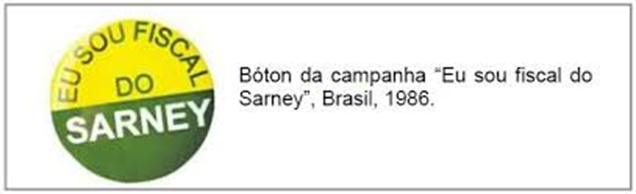
\includegraphics[width=0.7\linewidth]{Imagens/a11i1.png}
\end{figure}

\textbf{\textit{Fracasso}}\begin{itemize}
    \item \textbf{Congelamento de preços ou a política monetária acomodativa?} \begin{itemize}
        \item Intensidade do efeito riqueza(percepção da população que a moeda(poder de compra) está mais estável) foi significativa, de modo que, diante do abono(formula salarial não gerou arrocho) e das políticas expansionistas, houve superaquecimento da economia;
        \item Houve saque significativo da poupança (ilusão monetária); com essa queda abrupta da inflação, se perdeu a noção do que é real (rendimento líquido) para o nominal(rendimento bruto (inflação + real)), as pessoas viram uma queda do rendimento da poupança, as pessoas sacaram os valores da poupança. O que aumento a liquidez da economia, aquecendo a economia.
        \item Foco foi exagerado no problema inercial, faltando medidas de suporte para sustentar a inflação em patamar baixo (congelamento de preços);
        \item Política monetária ativa com juros altos, ajuste fiscal forte e ausência de abono salarial são exemplos de suporte para o congelamento (lógico que todos tem problemas);
        \item O congelamento, além de ser um instrumento ineficaz (desde o seu ponto de partida), trazia desequilíbrios e não contou com medidas para minimizar o conflito distributivo. E isso se tornou uma bomba relógio para isso se refletir no conflito distributivo.
    \end{itemize}
    \item \textbf{Resultado:} \begin{itemize}
        \item O superaquecimento da economia gerou desabastecimento (importados não minimizaram a situação, pois a economia brasileira era fechada; tudo em todos os lugares tinham limites de compra);
        \item Isso reforçou o conflito distributivo (desequilíbrios; todos os agentes estão tentando recompor seus preços para o valor que eles achavam justos) e tensionou o congelamento.
    \end{itemize}
    \item \textbf{Consequências}:\begin{itemize}
    \item Agravamento do processo inflacionário:\begin{itemize}
            \item Gatilho tornou endógeno aos salários os reajustes passados. A inflação voltou a ser um problema 
        \end{itemize}
    \item Os planos de estabilização seguintes perderam a credibilidade perante os agentes e a população. De uma hora para outra a inflação reduziu, a economia aqueceu, o mercado de trabalho estava a 100\%, mmomentos depois, tudo isso vai a ruína;
    \item Câmbio nominal fixo (uma escolha do Plano Cruzado) diante da demanda aquecida e do retorno da inflação doméstica, deteriorou a balança comercial.\begin{itemize}
            \item Setor externo deteriorou e o Brasil não pagou suas obrigações externas, decretando moratória da dívida externa em 1987 (a situação que não chegou nos anos 80, aconteceu agora). Consequência disso, fim de financiamentos externos para atender demandas nacionais, uma medida para tentar suprir isso seria uma balança comercial muito grande (\(EX_{BR} \gg IM_{BR}\)).
         \end{itemize}
    \end{itemize}
\end{itemize}

\subsection{\textbf{Plano Bresser}}

\begin{figure}[H]
    \centering
    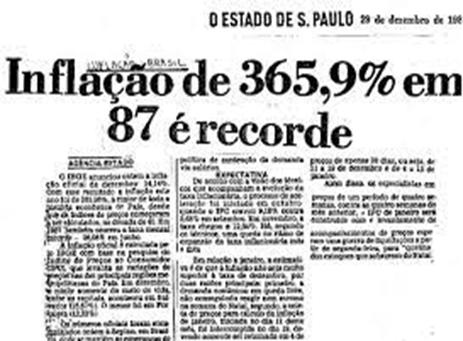
\includegraphics[width=0.7\linewidth]{Imagens/a11i2.png}
\end{figure}

Nomeação do economista e ministro da Fazenda do Brasil, nomeado pelo Sarney.

A inflação tinha causas inerciais e de demanda.

Anunciado em junho de 1987 (Ideias da FGV-RJ), o plano seria híbrido: com traços ortodoxos e heterodoxos.\begin{itemize}
    \item A ideia não era eliminar a inflação e a indexação abruptamente, mas reduzir o patamar da inflação e reduzir o déficit público.
    \item No geral, tentar corrigir algumas falhas e exageros do Plano Cruzado.
\end{itemize}

\subsection{\textbf{Plano Bresser (1987): uma síntese}}

Houve congelamento de preços (tal como o Cruzado, seguindo a linha heterodoxa):
\begin{itemize}
    \item Por um tempo menor (3 meses) e com ajuste prévio dos preços públicos; o Plano Cruzado fixou praticamente 1 ano com esse congelamento e sem perspectiva de descongelamento.
    \item Salário foi congelado por 3 meses.
\end{itemize}

Câmbio não foi congelado (outra diferença entre ele o o Pano Cruzado): foi desvalorizado e seguiu com minidesvalorizações (com velocidade menor, indicando inflação futura menor).

Políticas monetária e fiscal foram ativas e contracionistas.

\textbf{Fracasso (no mesmo ano)}:\begin{itemize}
    \item Houve recessão (devido a essas medidas) e Bresser (o ministro) não contou com apoio político para emplacar sua reforma administrativa; dado que ele defendia uma grande reforma administrativa e tributária e não houve apoio, o que impediu de se realizar o ajuste fiscal que, de acordo com ele, iria ajudar na manutenção da inflação.
    \item Vários itens foram liberados do congelamento, dada a pressão inflacionária, o que abalou a credibilidade do plano, gerando seu fracasso.
\end{itemize}

\subsection{\textbf{Plano Verão ((1989))}}
\begin{figure}[H]
    \centering
    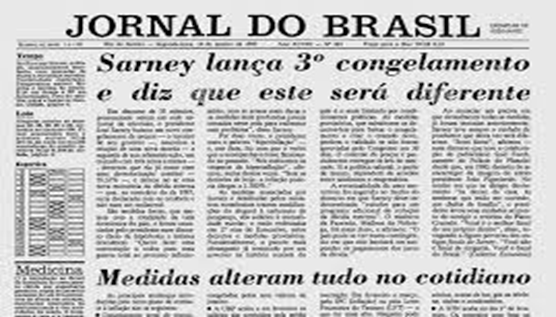
\includegraphics[width=0.7\linewidth]{Imagens/a11i3.png}
\end{figure}

Em janeiro de 1989 ocorre mais uma reforma monetária que institui o cruzado novo (NCz\$), equivalendo a mil cruzados. Dá seria "mais uma vez a mesma tentativa, mas vai diferente dessa vez"

Foi um plano híbrido(medidas heterodoxas e ortodoxas):
\begin{itemize}
    \item Conter demanda com taxas de juros reais elevadas e cortes nas despesas públicas(ortodoxia);
    \item O aspecto heterodoxo foi promover uma desindexação arrojada, suspendendo e extinguindo mecanismos de retroalimentação inflacionária(heterodoxia);
    \item Houve congelamento dos preços por tempo indefinido(outra semelhança com o plano cruzada ; antes foram autorizados aumentos dos preços públicos e câmbio em 1US\$ para 1 NCz\$).
\end{itemize}

\subsection{\textbf{Plano Verão (resultados)}}
Desejava promover dois ou três meses de inflação baixa com a economia desindexada: convenceria os agentes a ampliar as periodicidades de reajustes futuros.

A lógica era razoável, mas faltava credibilidade após uma sequência de planos fracassados.

O descongelamento foi gradual e cheio de regras, não tardou a gerar elevação da inflação(lembrando da moratória da dívida externa que foi declarada em 1987):
\begin{itemize}
    \item 30\% em agosto passou para 50\% em dezembro, caminhou para 70\% e atingiu um pico de 84\% em fevereiro e março de 1990 (4.800\% anualizados!);
    \item Deixou a economia brasileira com grau de indexação superior ao pré-Plano.
\end{itemize}

\newpage
\section{\textbf{As tentativas de estabilização Parte II (1990-1994) : Planos Collor}}
\subsection{\textbf{Introdução}}
\textbf{Temas}
\begin{enumerate}
    \item Planos Collor (I e II).
    \item O Plano Collor foi ortodoxo ou heterodoxo?
\end{enumerate}

\textbf{O que é mais importante?}

Identificar as medidas, os instrumentos e o fracasso do Plano Collor.

\textit{Leitura: Ordem do Progresso e Economia Brasileira Contemporânea (trechos sobre o Plano Collor)}
\begin{figure}[H]
    \centering
    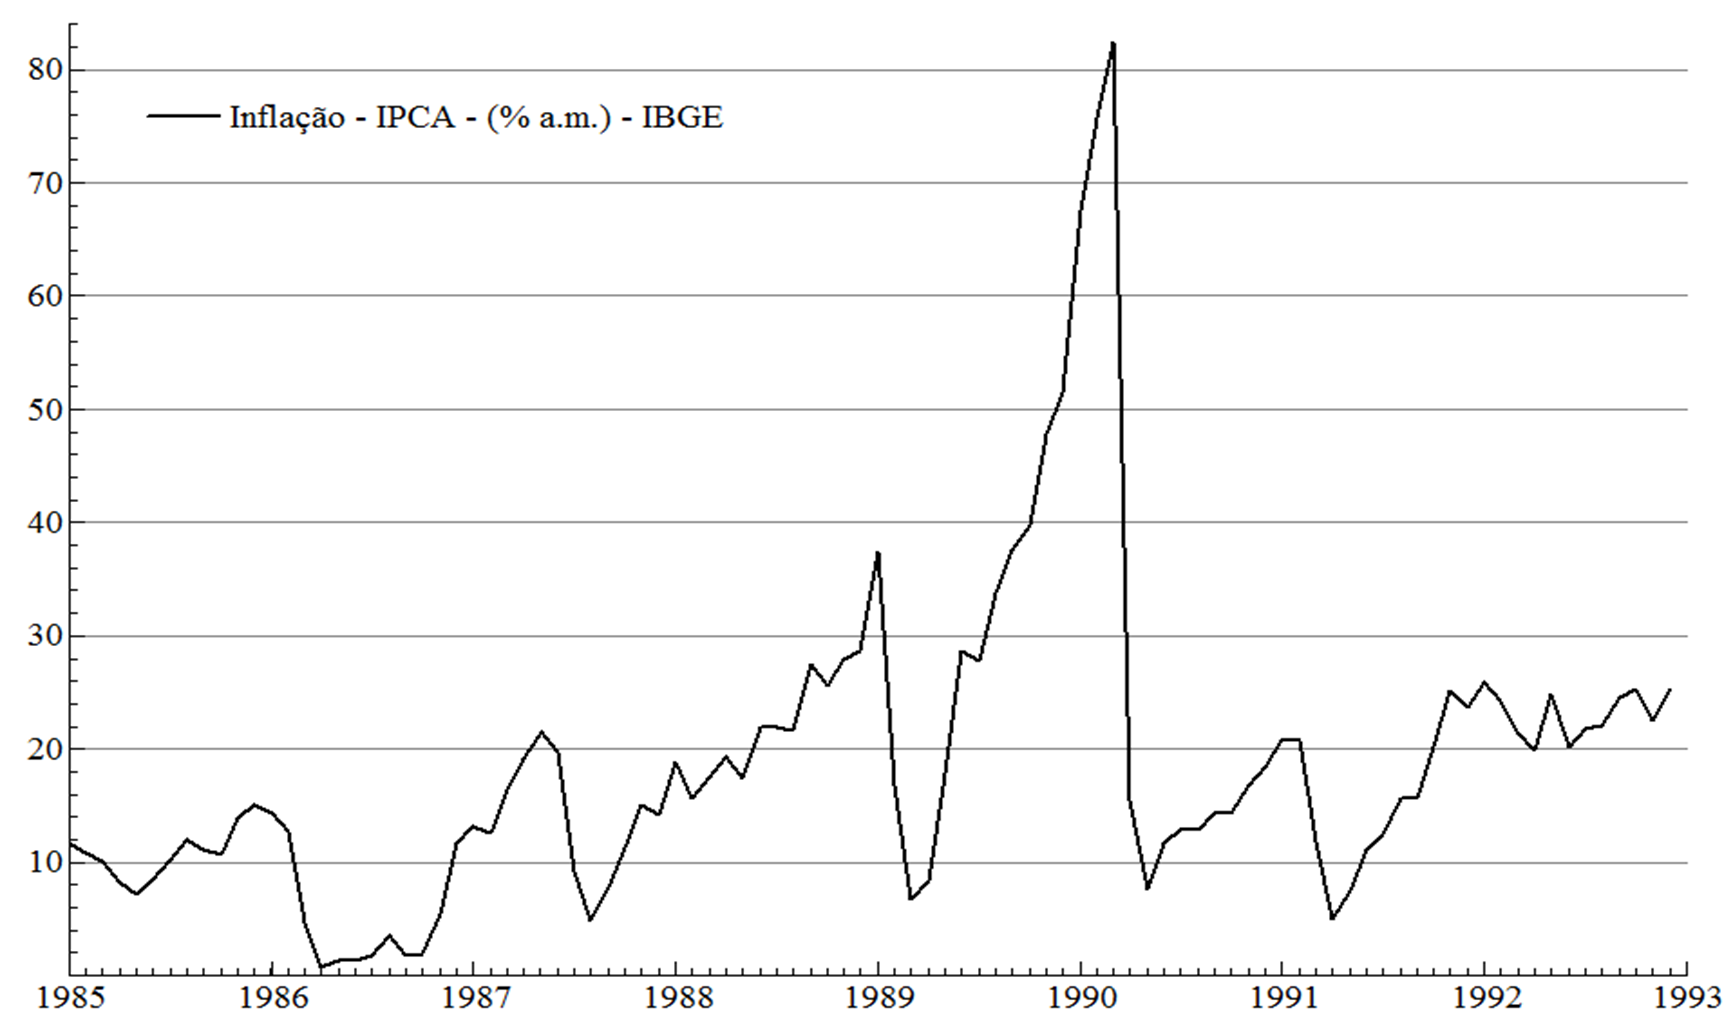
\includegraphics[width=0.7\linewidth]{Imagens/a12i1.png}
\end{figure}

\subsection{\textbf{Síntese do período 1990-1994}}
Fernando Collor assume em 15 de março de 1990, anunciando drástico plano de estabilização, dada a inflação mensal de 80\%.

\begin{itemize}
    \item O plano fracassou, mas trouxe o debate e encabeçou medidas de privatização e de abertura comercial(um dos planos mais bizarros, jogou o Brasil em dois anos de recessão; ideias de Margareth Tatcher e Ronald Regan);
    \item Collor sofreu impeachment em 1992 e Itamar Franco(seu vice), após grande volatilidade inicial(inflação altíssima), nomeou FHC em 1993 para a Fazenda, que lideraria a implementação do Plano Real em 1994.
\end{itemize}

\subsection{\textbf{Contexto em 1990}}
Collor vence Lula nas eleições com o seguinte discurso:
\begin{itemize}
    \item Lula romperia contratos(de acordo com o Collor);
    \item Era de "fora" da política;
\end{itemize}

Temia-se congelamento por parte dos agentes(presidente novo, política velha). Houve forte especulação e remarcações preventivas, agravando ainda mais a conjuntura.

\subsection{\textbf{Lógica principal do plano Collor}}
O Cruzado havia sido precedido de amplo debate e por uma série de estudos de diagnóstico e propostas de desindexação, fazendo a "sociedade" compreender melhor. Isso não ocorreu com o Plano Collor, tornando-o de difícil avaliação(até para economistas era difícil entender o Plano Collor).

\textbf{Ideia do confisco(quase 80\% dos ativos) parece ter surgido em “Crise e reforma monetária no Brasil” (Belluzzo e Júlio Almeida)}. A grande medida do Plano Collor.
\begin{itemize}
    \item Circulou 1º na equipe de Ulysses Guimarães (que perdeu no 1º turno) e depois chegou a Kandir da assessoria de Lula. Kandir estava na coletiva do anúncio do Plano Collor ao lado de Zélia Cardoso de Melo;
    \item Muitos acreditavam que algo drástico tinha de ser feito;
    \item Mesmo M. H. Simonsen(o mesmo de eras atrás e convidado pelo Collor para avaliar o PLano Collor) achou a ideia boa, mas duvidou da capacidade de algum presidente de executar essa medida.
\end{itemize}

\textit{Referência importante: Pastore, A. C. A reforma monetária do Plano Collor. Revista Brasileira de Economia. 1991.} Um dos poucos economistas da época que de fato entendeu o Plano Collor, e nesse trabalho, Pastore apontou qual o defeito desse grande plano.

\subsection{\textbf{Elementos gerais do Plano Collor}}
Reforma monetária retira os \underline{cruzados novos} e reintroduz o \underline{cruzeiro}(de novo uma mudança de novo)

\begin{itemize}
    \item Houve congelamento (salários somente reajustaram até fevereiro, perdendo no meio março);
    \item Mas a falta de credibilidade desse instrumento, trouxe desrespeito e pouco caracteriza o Plano.
\end{itemize}

\textbf{O diagnóstico da inflação:}
\begin{itemize}
    \item Além do tradicional descontrole(excessos) monetário e fiscal;
    \item Tinha origem na possibilidade de rápida monetização das aplicações financeiras;
    \item As operações de overnight(causas da rápida monetização; essas operações não são do Plano Collor, mas sim uma forma de definição da taxa de juros) fixavam a taxa de juros com base na inflação(de quase 3000\% ao ano da época).
\end{itemize}

\subsection{\textbf{Como funcionavam as aplicações de overnight e qual a relação com o processo inflacionário?}}
Agentes buscam proteção contra inflação altíssima: Normalmente os depósitos bancários estavam vinculados a aplicações que rendiam juros diários (operações overnight com juros diários, a custo zero, com qualquer dinheiro que "pingava" na conta);

Essas aplicações estavam vinculadas ao mercado de títulos públicos e privados(local onde a taxa de juros é definida);

Bacen fixava a taxa de juros overnight acima da inflação; na época a taxa de juros overnight girava entorno de 1,7\% ao dia, na conta o rendimento em contas girava em torno de 1,8\%, isso capitalizado ao ano dava 469,05\% do Bacen, dos depósitos girava entorno de 671.88\% ao ano.

Ao longo do dia o Bacen entrava vendendo/comprando títulos para avaliar o mercado (GO AROUND);

Se o setor privado não exercesse a fluidez no mercado de títulos, o Bacen faria obrigatoriamente a recompra de títulos, garantindo a operação. (era a \textit{zeragem automática})

A garantia da zeragem deixava a operação líquida e \underline{risco nulo para a alavancagem bancária!}

Como a conversão das aplicações em M1, moeda, não tinha custo tal mecanismo era gerador de moeda.

Participação de cada agente: Os bancos ganham nas operações com títulos, os clientes protegem-se da inflação e o Bacen mantem essa operação.

Dessa forma, tal procedimento agrava a indexação, gerando a “moeda indexada”.

\subsection{\textbf{Diagnóstico}}
O Brasil tinha perdido quase todos os instrumentos de política econômica ao longo da década de 1980.

\begin{itemize}
    \item Fixava a taxa de juros alta, pois seu setor fiscal desestruturado e dívida crescente exigiam, assim perdia o controle sobre o crescimento dos agregados monetários;
    \item Restava interferir no mercado de títulos onde, dada a incerteza inflacionária gigantesca, exigia-se taxas formadas diariamente que se baseavam na inflação passada;
    \item Assim, a oferta monetária crescia indexada na inflação; assim o governo fica de mãos atadas
    \item A partir desse raciocínio se estabeleceu a medida mais importante do plano Collor, bloqueio de liquidez (confisco de ativos) –\textbf{ popularmente confisco da poupança (e outras aplicações financeiras)}.
\end{itemize}

\textbf{Outros pontos importantes}: Política Fiscal/Reforma administrativa; O fracasso do Plano e as críticas.

\textit{Anúncio do Confisco das Poupanças} (\href{https://www.youtube.com/watch?v=7KhZa2R-C-E}{link para o vídeo}).

\subsection{\textbf{Confisco (dentro da reforma monetária)}}
Depósitos maiores do que 50 mil cruzados novos (1200 dólares da época) seriam depositados no Bacen e devolvidos em parcelas 1,5 anos depois com juros e correção. Isso \textbf{somente} no dia 16 de março de 1990(um dia depois da posso do Collor). Os dias seguintes foi "normal". Postere falou que isso foi um \textbf{confisco que estoque}. Cerca de 100 bilhões de dólares foram confiscaram nesse dia. 

\begin{itemize}
    \item Sequestro de 70/80\% do M4(agregado monetário bastante amplo, de alta e baixa liquidez) e seria a grande âncora do plano(e lá se foi o overnight);
    \item A indisponibilidade de M4 reduziu a quantidade de moeda, M1, e a quantidade de todos os demais ativos financeiros;
\end{itemize}

\textbf{Qual era a lógica dessa medida?}
\begin{itemize}
    \item Evitar saques fortes de aplicações financeiras, tentando evitar a “ilusão monetária” que motivou saques da poupança no Plano Cruzado; E o Plano Collor não queria isso, pois assim iria axistir uma pressão devido ao aumento de liquidez.
    \item Confisco + contenção da demanda agregada + política fiscal contracionista apoiariam o congelamento, o que permitiria alcançar o fim da indexação;
    \item Desindexar a economia, freando a “moeda indexada” presente na dinâmica das aplicações financeiras diárias de overnight.
\end{itemize}

\textbf{Item inercial também existiu dentro do diagnóstico do Plano Collor!}

\subsection{\textbf{Erro de diagnóstico da equipe econômica}}
Mas o efeito inflacionário deste processo não reside no rendimento que é diário, mas na garantia de recompra do BC (zeragem) que é um fluxo. (Teoria Quantitativa da Moeda)

Base monetária e M1 ainda cresciam passivamente tanto quanto antes da reforma monetária e do confisco

O Plano sequestrou o estoque e promoveu medidas de congelamento e de ajuste fiscal. Assim se preocupou com a variável estoque.

Mas ele deveria ter acabado com o mecanismo de \textit{zeragem automática, o fluxo da operação que deixava bancos alavancados e com risco zero. Não foram criadas regras e mecanismos tentando acabar com essa dinâmica de criação de moeda.}

\textit{Haveria de ter sido criado um regime monetário que permitisse o controle da base monetária e de M1.}

\subsection{\textbf{Política fiscal/ Reforma Administrativa}}
\textbf{Objetivo: reduzir o déficit público}\begin{itemize}
    \item Enxugar e modernizar a máquina pública, reduzindo número de ministérios, extinguindo institutos, cortando verbas, propondo plano de demissão de funcionários públicos;
    \item Promoveu aumentos do IPI, IOF (peso importante, quase zerou o déficit em 1990);
    \item Reduziu ministérios (23 para 12). Ministra Zélia Cardoso acumulou Fazenda e Planejamento;
    \item A ideia era fazer uma “devassa” no setor público, reduzindo a sonegação e as fraudes. Isso aumentaria a eficiência administrativa e reduziria os gastos.
\end{itemize}

Mas Collor não contava com 2/3 de apoio do Congresso, então não conseguiu aprovar boa parte de suas intenções que dependiam de mudanças de lei.

\subsection{\textbf{Resultados}}
Desespero, desconfiança e descontentamento. Trabalhadores e empresários foram surpreendidos. Principalmente na medida do confisco.

Houve efeito riqueza negativo: sensação dos agentes era de que o dinheiro não seria mais devolvido, apesar da inflação, ao mês, ter caído de quase 70\% para praticamente 0\%.

Faltava capital de giro para as empresas, havia situações dramáticas em algumas famílias.

Houve fortes pressões políticas/jurídicas sobre o Bacen, de modo que a proporção de ativos retidos reduziu bastante ao longo do tempo.

Houve forte desestruturação do sistema produtivo

Confisco + Efeito riqueza negativo + Ajuste fiscal = forte recessão (os anos de 1990, 91 e 92 até o 4º trimestre datados como recessão)

\subsection{\textbf{Plano Collor II}}
Em 1991, houve anúncio de outro plano (sim, mais um) de estabilização com novo congelamento de preços(sim, de novo).

\begin{itemize}
    \item Houve forte resistência do Congresso e nem mesmo conseguiu aprovar uma proposta de reajuste salarial.
\end{itemize}

\textbf{A ideia desse plano seria acabar com a indexação no mercado financeiro(a mesma ideia do Collor I, porém de forma diferente), como?}
\begin{itemize}
    \item Governo acaba com o BTN (Bônus do Tesouro Nacional), que era a base lógica das operações do overnight para formação da taxa de juros;
    \item Substitui a BTN pela FAF (Fundo de aplicações financeiras), que rende TR (Taxa Referencial);
    \item A TR (baseada na média formada no mercado interbancário) inclui no jogo expectativas futuras (\textit{forward looking}), fazendo a inflação ficar baseada em movimentos futuros, não mais para o passado inflacionário problemático. Tudo isso para tentar enfraquecer a memória inflacionária.
    \item Isso deixava o passado menos importante (memória com peso pequeno) na formação do processo inflacionário;
    \item Agentes olhariam o lado fiscal e, se esse fosse bem conduzido, geraria expectativas de inflação menores;
    \item Melhoraria fundamentos macro(dado as melhorias dessas outras variáveis(câmbio, juros, inflação, etc)) e causaria nova melhoria fiscal, o que baixaria a expectativa de inflação gradualmente (ciclo virtuoso);
    \item Gustavo Franco chamou de “\textbf{neogradualismo}”(referência aos planos gradualistas de redução de inflação passados);
    \item A ideia era razoável, mas a sequência de crises políticas tirou qualquer probabilidade de sucesso. Gerando mais um fracasso de mais um plano de estabilização.
\end{itemize}

Zélia Cardoso foi substituída por Marcílio Marques Moreira em maio de 1991 (lembrando que o Collor assumiu em março de 1990 e tudo isso começou a quase um ano).

\subsection{\textbf{Plano Collor: ortodoxo ou heterodoxo?è difícil dizer}}
Pessoas próximas ao Collor, diferente das Críticas do Pastore, afirmavam que o Plano Collor só deu errado porque os agentes políticas não apoiavam as medidas do redução de liquidez. Permitindo que a liquidez que era para ter ficado restrita por mais tempo, mas decisões permitiam devolução de parte do confisco antes do prazo, o que prejudicou o processo de estabilização. 

O monetarismo(como muitos economistas da época chamavam esse plano, logo um plano ortodoxo), acima de tudo, tem apoio na soberania do mercado. Mas as decisões e como foram tomados não podem ser chamadas de totalmente ortodoxo\begin{itemize}
    \item O plano Collor fez forte intervenção estatal (houve confisco de patrimônio; só esse ponto era ortodoxo e ponto final);
    \item Não basta, assim, os aspectos do controle monetário e de privatizações.
\end{itemize}

\textbf{A teoria inercialista(heterodoxo)}, por outro lado, apoia-se no conflito distributivo:\begin{itemize}
    \item Conflito entre salário/lucro nas negociações trabalhistas gera a formação de preços (mercado de trabalho importa);
    \item Nesse processo está a raiz da inércia; mas não era só lá que havia conflito distributivo, mas foi esse o ponto que eles se apoiaram
    \item Mas não incorpora o aspecto financeiro (por exemplo, o financiamento dos estoques das dívidas externa e interna pouco foram objetos dos planos heterodoxos – exceto na visão de Bresser).
\end{itemize}

\textbf{Nesse sentido, o Plano Collor é eclético(Pedro Fonseca, um economista do sul classifica dessa forma)!}
\begin{itemize}
    \item Procura incorporar o mercado financeiro (dinâmica da dívida externa e interna importa, dada a formação de juros no \textit{overnight});
    \item Para se financiar, o governo fixa as taxas de juros, que alimentam a dinâmica do mercado financeiro;
    \item O descontrole da inflação está no mercado financeiro! (justifica medidas sobre aplicações financeiras);
    \item Também o controle do déficit público é fundamental (de fato, onde está a raiz da inflação; o problema mestre é o problema fiscal, algo que é apontado e elogiado pelo próprio Pastore, o próprio afirma que ele errou onde aplicar a medida).
\end{itemize}

\newpage
\section{\textbf{Reformas Estruturais no Início dos Anos 1990 e o Plano Real}}
\subsection{\textbf{Introdução}}

\textbf{Temas}\begin{itemize}
    \item Reformas estruturais na primeira metade dos anos 1990.
    \item Introdução ao plano Real. 
    \item Plano Real - Discussão [Leitura: Giambiagi, cap. 6, trecho O Plano Real: concepção e prática; Ordem do Progresso, cap. 15, trecho concepção e implementação do Plano Real]. 
\end{itemize}

\textbf{O que é mais importante?}\begin{itemize}
    \item Identificar os diferenciais entre o contexto, as medidas e os instrumentos do Plano Real em relação aos planos anteriores, explicando seu sucesso
    \item Leitura: Ordem do Progresso (cap. 15 ) e Economia Brasileira Contemporânea (cap. 6)
\end{itemize}

\subsection{\textbf{Reformas estruturais dos anos 90}}
No contexto de início dos anos 1990, três processos foram importantes para a economia brasileira: abertura comercial, renegociação da dívida externa e privatizações. \begin{itemize}
    \item Substituir a PSI pela PICE (Política industrial e de Comércio exterior)
    \item A ideia era incentivar a competição, gerando ganhos de produtividade, algo bem diferente da agenda anterior, um Brasil quer entrar não 
    \item Implementar o PND (Plano Nacional de Desestatização(Privatização); não o dos anos 80)\begin{itemize}
        \item Incentivar o desenvolvimento privado
        \item Redesenhar o parque industrial;
        \item Reduzir a dívida pública;
        \item Principais setores: siderurgia, petroquímico e fertilizantes.
    \end{itemize}
\end{itemize}

A abertura comercial(lembrando que desde do PAEG o Brasil não era aberto para o comércio) ocorreu em etapas, reduzindo a tarifa média nominal de 58\% para 32\%.\begin{itemize}
    \item Produtos importados aumentam a competição interna, reduz custos de bens nacionais, incetivos(indiretos) para o desenvolvimento de melhores produtos nacionais.Lembrando que o Brasil vivia a hiperinflação, e com a abertura comercial poderia desacelerar a inflação nacioanl. 
    \item o arcabouço institucional antigo de controle das importações (licenças, proibições e os regimes especiais), utilizados desde a década de 1940, foi derrubado no período de 1990-93, algo construído desde o governo de Getúlio Vargas
    \item isso tenderia a alavancar a participação das importações no PIB brasileiro.
\end{itemize}

As privatizações(de empresas nacionais antigas; mas os agentes desses setores reclamaram bastante dessa medida) foram comandadas pelo BNDES, seguindo regras claras e procedimentos detalhados. \begin{itemize}
    \item Envolveria, em um primeiro momento, empresas mais conectadas com uma estrutura de mercado competitiva, como de mineração e siderurgia;
    \item Outras, em um segundo momento, de monopólio natural como teles e elétricas que exigiriam implantação de agências reguladoras com credibilidade e transparência;
    \item foram privatizadas(escolhas de um governo/país de mais liberalizante, ambos(estado e setor privado) tem interesse com isso, isso ajuda o governo a mobilizar recursos financeiros estrangeiros), ainda sob governos Collor e Itamar, empresas como: CSN (primeiro grande investimento industrial do estado brasileiro ainda na II GM) e Usiminas.
\end{itemize}

Plano Brady (reestruturação/renegociação da dívida externa(melhorar as condições da pagamento dessa dívida))\begin{itemize}
    \item Em julho de 1992 foi assinado um acordo com os credores privados (negociação liderada por Pedro Malan(futuro integrante do Plano Real));
    \item Depois de um processo que vinha se arrastando desde a década de 1960 e havia se agravado com a moratória de 1987; Isso acaba com investimento estrangeiro direto da época e nas épocas seguintes. 
    \item A  ideia seria diminuir seu valor e seu serviço, reduzindo o risco da dívida brasileira; isso melhora as condições de pagamento dessa dívida
    \item Poderia gerar novo cenário de investimentos estrangeiros. Dada redução dos juros internacionais e o Brasil com juros altíssimos, isso faz com que o Brasil volta a receber investimento externo, a conta capital volta a ter relevância
\end{itemize}

\subsection{\textbf{Implementação do Plano Real}}
Antes de suas três grandes fases, foi fundamental para seu sucesso e implementação inicial:\begin{itemize}
    \item As reformas dos anos 90, em síntese favoreceriam o Plano Real;
    \item impostos menores sobre as importações(com a Abertura Comercial)
    \item consumidores de bens importados pagam menos; exportadores barganham melhores taxas com outros países; 
    \item as privatizações, potencialmente, trariam impactos positivos fiscal e no balanço de pagamentos;
    \item A renegociação da dívida externa tenderia a reintroduzir a importância da conta de capitais.
\end{itemize}

As medidas de política econômica não repetiriam ações do passado como congelamentos de preços e salários, confiscos etc. O aprendizado com os erros de planos anteriores seria vital e moldaria boa parte das ações do Real. Depoimento de FHC sobre o plano (\href{https://www.youtube.com/watch?v=K_PhYIs5FLc}{vídeo} a partir de 3´00). Em 1993 a inflação mensal já chegava na casa dos 30\%, as dificuldades seriam enormes. Caberia a FHC:\begin{itemize}
    \item recrutar equipe competente (com a pressão e expectativa de curta duração no governo seria difícil o recrutamento);
    \item traçou um acordo com a equipe de não interferência técnica e que regras não hierárquicas seriam respeitadas, como um indivíduo se sobrepor a ideia do grupo;
    \item exercitar a habilidade para buscar apoio dentro do governo, Congresso e da opinião pública, convencendo que esse plano seria diferente dos demais;
    \item Vídeo Lançamento do Plano Real - 01.07.1994 (\href{https://www.youtube.com/watch?v=Wxq6WbD8tw4}{vídeo})
    \item Depoimentos da equipe (\href{https://www.youtube.com/watch?v=AlFOWRIdyao}{vídeo})
\end{itemize}

\subsection{\textbf{Medidas do Plano Real}}
Em 1993, foi anunciado que o plano seria composto de três etapas:\begin{enumerate}
    \item Forte ajuste fiscal que seria negociado com o Congresso;\begin{itemize}
         \item reconhecida a necessidade de reformas da Previdência e tributária, além dos “esqueletos”, sobras de outros planos e a necessidade de imposição de disciplina fiscal aos estados e municípios. Sabia-se da dificuldade de implementação no curto prazo.
         \item tributou o sistema financeiro e estabeleceu o FSE (Fundo Social de Emergência) que reduziria a rigidez orçamentária. Essas medidas, em conjunto com os efeitos da inflação, geraram superávits fiscais significativos (5,1\% do PIB em 1994)
     \end{itemize}
     \item Seria criada a URV (Unidade real de valor), unidade de conta com reajuste diário que conviveria com o cruzeiro real\begin{itemize}
         \item foi estabelecida uma paridade entre cruzeiro real e URV, assim os preços relativos seriam todos regidos por essa unidade, evitando distorções e períodos de transição
         \item todos os novos contratos seriam em URV e os contratos antigos seria de escolha dos agentes converter. (quando o real fosse criado em julho, a conversão seria obrigatória)
         \item isso estimulou livre negociação entre os agentes para converter contratos em URV (seria um pacto social individualizado, descentralizado, sem tentativas hierárquicas para estabelecer conversões)
     \end{itemize}
     \item Reforma monetária que excluiria o cruzeiro real, transformando-o em real o que significaria conferir a URV a função de meio de pagamento.\begin{itemize}
         \item isso (livre negociação) deu suavidade ao processo de transição monetária. E no dia da transição, a URV, ou seja, o real, era equivalente a 2750 cruzeiros reais. E um real era igual a um dólar nesse dia
         \item a inflação de 10\% em julho foi para 1\% no final do ano.
         \item Para o plano ser um sucesso, foram visualizadas mais de uma “âncora”:\begin{itemize}
             \item a taxa de câmbio que estava protegida por um volume alto de reservas internacionais
             \item a “âncora” fiscal com a menor rigidez orçamentária pelo FSE
             \item intenções de manterem taxas de juros elevadas.
         \end{itemize}
     \end{itemize}
\end{enumerate}

\subsection{\textbf{Fases do Plano Real e a evolução mensal da inflação}}
\begin{figure}[H]
    \centering
    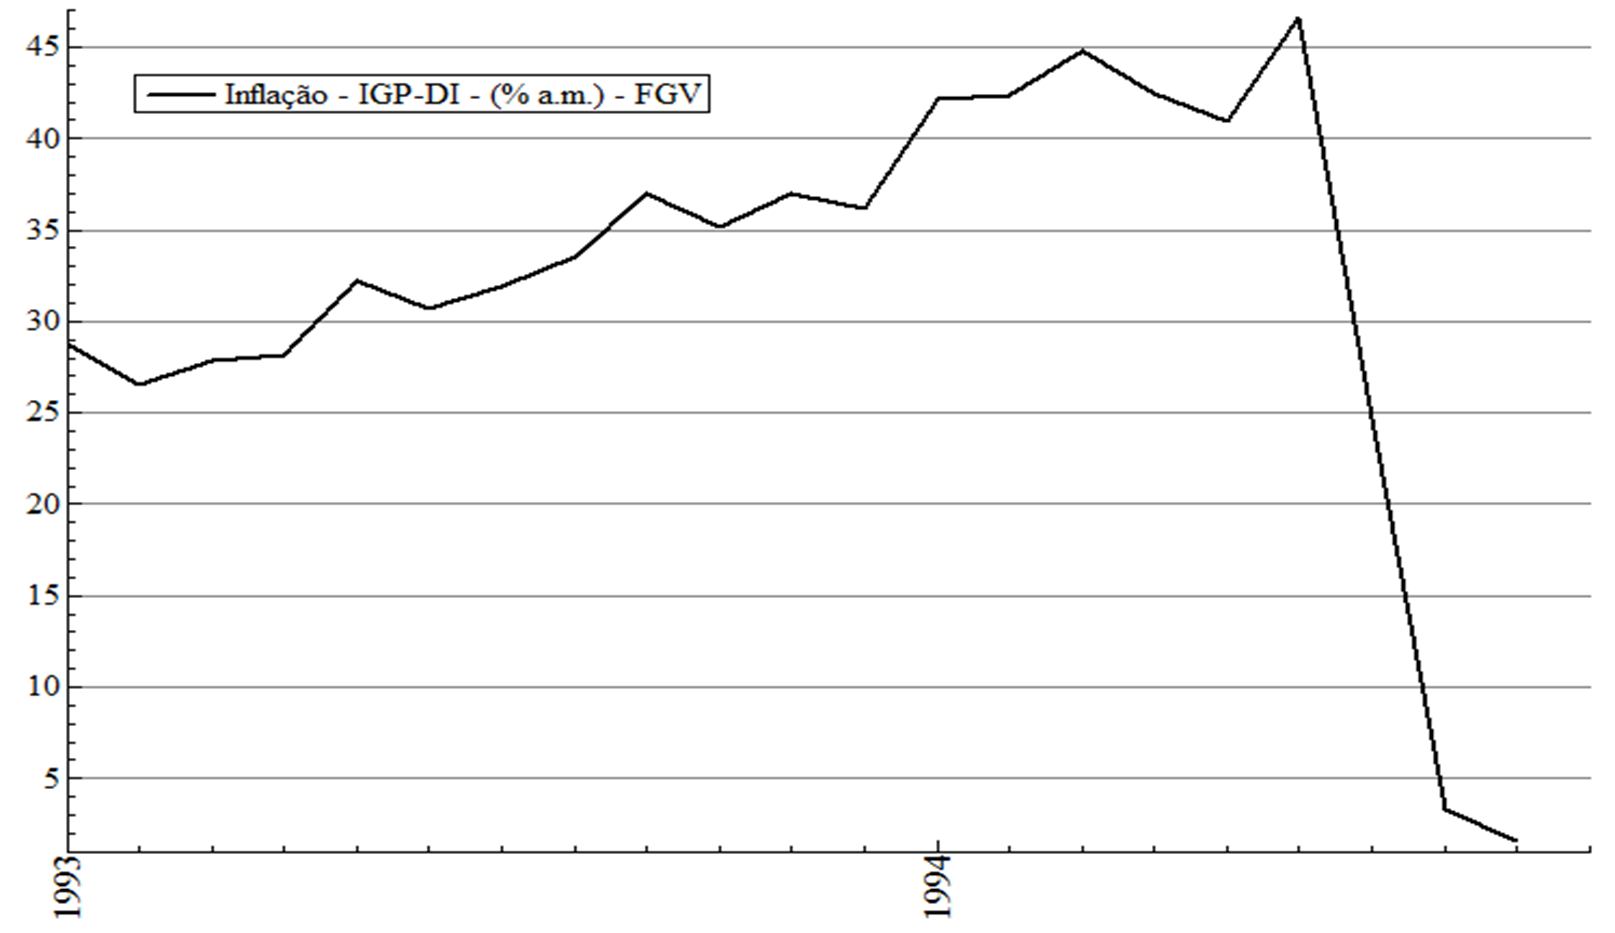
\includegraphics[width=0.7\linewidth]{Imagens/a13i1.png}
\end{figure}

\subsection{\textbf{Indexação e inflação}}
De fato, o grande problema é eliminar a inflação. Por que é ela que potencializa a indexação \begin{itemize}
    \item é fundamental controlar a indexação, mas o combate à inflação deve ser a preocupação central e a mais duradoura; 
    \item não é a indexação o problema primeiro, no fundo não é ela a causadora da inflação. 
\end{itemize}

O processo de indexação nessa etapa estava sem coordenação entre os agentes econômicos\begin{itemize}
    \item foi muito importante a transparência e a ideia de que não iria haver surpresas (como congelamentos etc); 
    \item isso levaria os agentes econômicos para um processo coordenado de indexação, sem defasagens de reajuste entre eles;
    \item na prática viabilizaria a eficácia da URV.
\end{itemize}

\newpage
\section{\textbf{Problemas econômicos e política econômica(O período FHC, 1995-2002)}}
\subsection{\textbf{Introdução}}
\textbf{Temas}
\begin{itemize}
  \item Os cenários externo e fiscal após a implementação do Plano Real
  \item Os regimes cambiais e a reação brasileira às crises financeiras/cambiais
  \item Política econômica após a crise cambial de 1999 \textit{(Discussão, leitura: \textbf{Ordem do Progresso} (cap. 16, trecho – Novo arcabouço de política econômica) e \textbf{Economia Brasileira Contemporânea} (cap. 7, trecho – O segundo governo de FHC: 1999–2002))}
\end{itemize}


\textbf{O que é importante?}
\begin{itemize}
  \item Estabelecer relações entre a estabilização e os setores externo e fiscal;
  \item Identificar e explicar a evolução do contexto cambial de 1994 até 1999 e as consequências sobre a condução da política econômica
\end{itemize}


\textbf{Leituras:} \textit{Ordem do Progresso} (cap. 16) e \textit{Economia Brasileira Contemporânea} (cap. 7)


\textbf{Texto de apoio:} PASTORE, Affonso Celso; PINOTTI, Maria Cristina. \textit{Inflação e Estabilização: Algumas Lições da Experiência Brasileira}. 

\textbf{Revista Brasileira de Economia}, Rio de Janeiro, v. 53, n. 1, p. 3–40, jan. 1999. Disponível em:\url{http://bibliotecadigital.fgv.br/ojs/index.php/rbe/article/view/747}. Acesso em: 30 abr. 2018.

A grande meta de FHC era consolidar o Real, garantindo a estabilização de preços(inflação baixa e estável nesse patamar)
\begin{itemize}
  \item Essa era a promessa de campanha e, por isso, foi eleito em 1º turno;
  \item FHC sabia que alianças políticas eram condição necessária para governar.
\end{itemize}

Pontos importantes para consolidar a estabilização(\textbf{A triade fundamental})
\begin{itemize}
  \item O câmbio deveria ser controlado em nível apreciado;
  \item As reservas internacionais deveriam efetuar esse controle;
  \item Juros deveriam ser mantidos em patamar elevado. Sua função era para reequilibrar o BP, via reservas internacionais.
\end{itemize}

\subsection{\textbf{Contexto econômico geral (1995-2002)}}
O “fim” da inflação evidencia outros problemas que desafiaram a condução da política econômica. Principais:
\begin{itemize}
  \item deterioração fiscal;
  \item dificuldades no sistema bancário, exigindo intervenção do BC;
  \item forte elevação dos déficits nas contas externas;
  \item enfrentou uma sequência de crises financeiras internacionais/cambiais (Crise do México, Crise da Ásia, Crise da Rússia(motivo que fez o Brasil abandonar o câmbio flutuante)); Teste de paridades ao longo do mundo, para aqueles países que seguiram o padrão brasileiro(câmbio administrado)
  \item passou por uma crise cambial com forte desvalorização (1999); O Brasil foi obrigado a abandonar a ancora cambial
  \item enfrentou um racionamento de energia e uma crise internacional (2001; crise da Argentina e atentado das Torres Gêmeas).
\end{itemize}

\subsubsection{\textbf{O contexto econômico inicial (final do governo Itamar Franco)}}
Há explosão do consumo pós lançamento do Real(era um trauma do Cruzado), dado o efeito riqueza. Aumento das importações, redução da arrecadação governamental, melhora das expectativas inflacionárias(o Brasil venceu a hiperinflação).

Estava em “gestação” a crise mexicana(dezembro de 1994, gerando efeito tequila e ele foi contagioso para outros países, devido a especulação no mercado financeiro) (crise no BP com forte desvalorização)\begin{itemize}
    \item Coloca forte risco aos países que seguem regimes cambiais controlados, dado a forte desvalorização do câmbio mexicano.
\end{itemize}

Reservas internacionais do Brasil sofrem queda, devido a incerteza desses regimes cambiais, os agentes econômicos procuravam o dólar por segurança.

Inflação estava resistente. E com a crise do México ele deu mais uma guinada

\textbf{Em síntese:} o cenário econômico era desafiador no primeiro semestre após o lançamento da nova moeda. Para agravar ainda mais, o governo FHC tem início com deterioração do BP e do quadro fiscal.

Por mais que o gráfico mostre uma inflação declinante, ela ainda é algo desconfortável e não pode ser deixada de lado. Lógico que milagres não acontecem, mas é um cenário delicado. Qualquer movimentação nas reservas internacionais é perigosa e devem ser controlada via taxa de juros.
\begin{figure}[H]
    \centering
    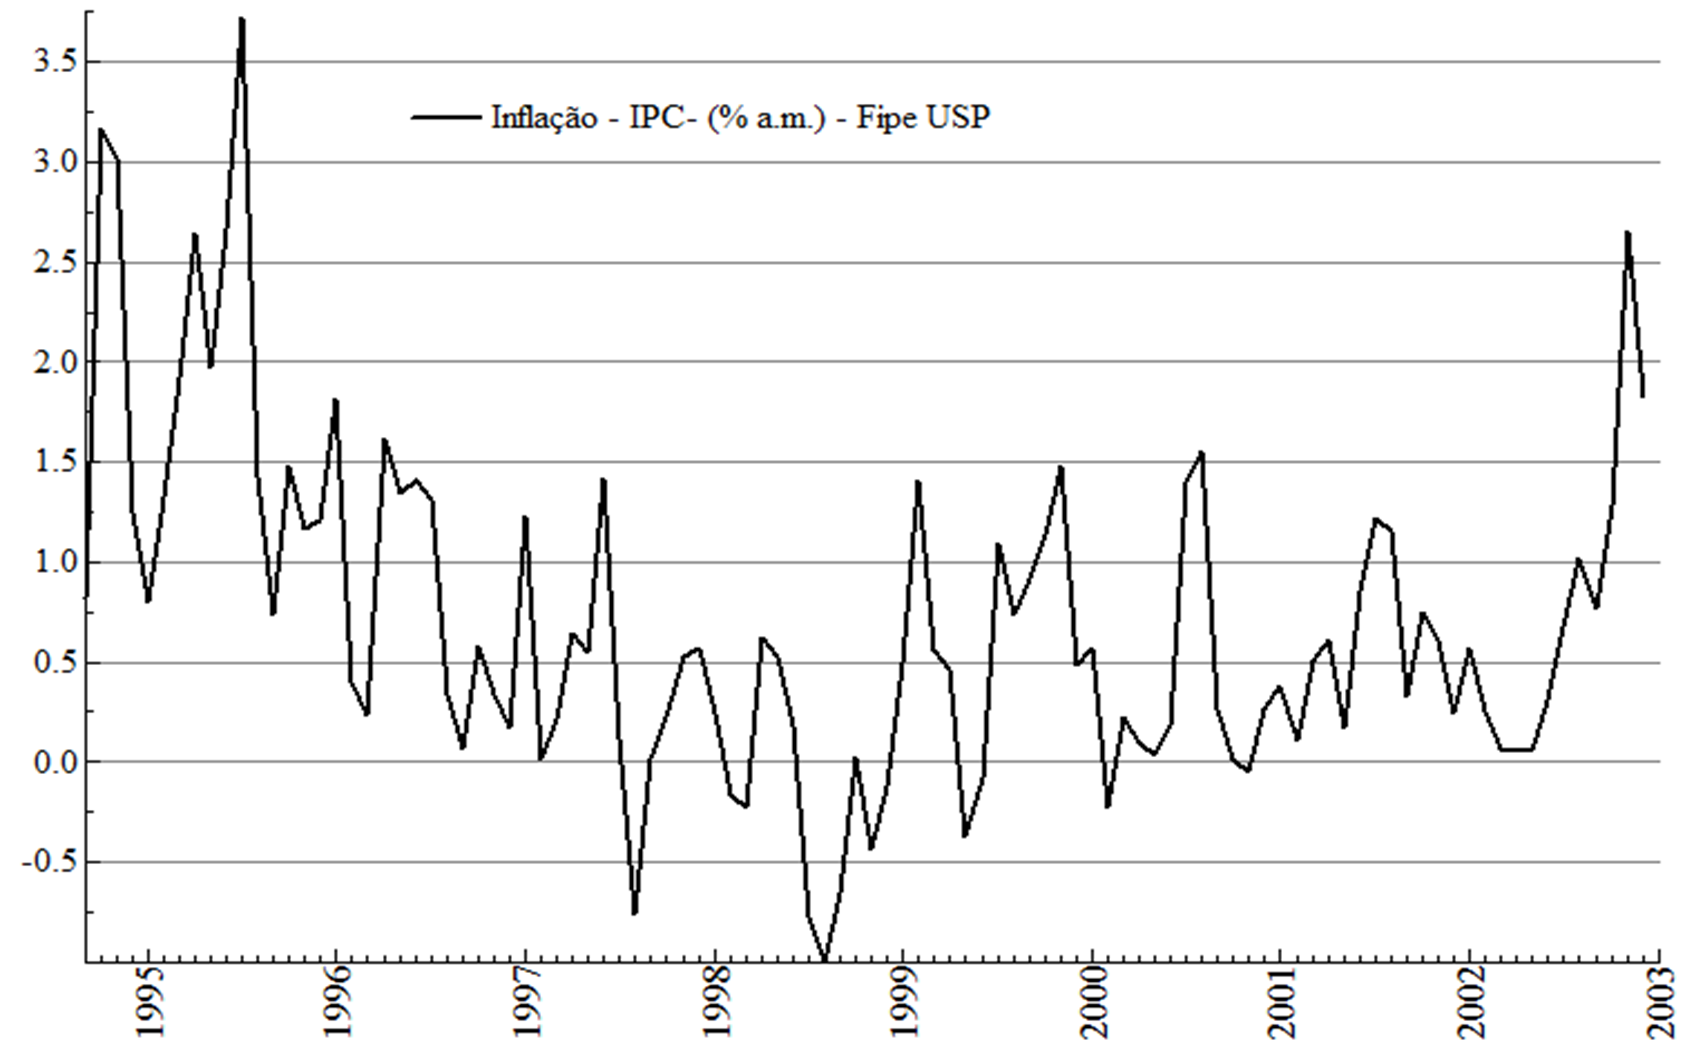
\includegraphics[width=0.7\linewidth]{Imagens/a14i1.png}
\end{figure}

Podemos ver que com o lançamento do Plano Real, os agentes estavam (menos o FMI) confiantes com esse palno, tanto é que as reservas nos primeiros meses do Plano Real, as reservas subiram. Quando as crises começaram, sentimos a perdas de reservas.

\begin{figure}[H]
    \centering
    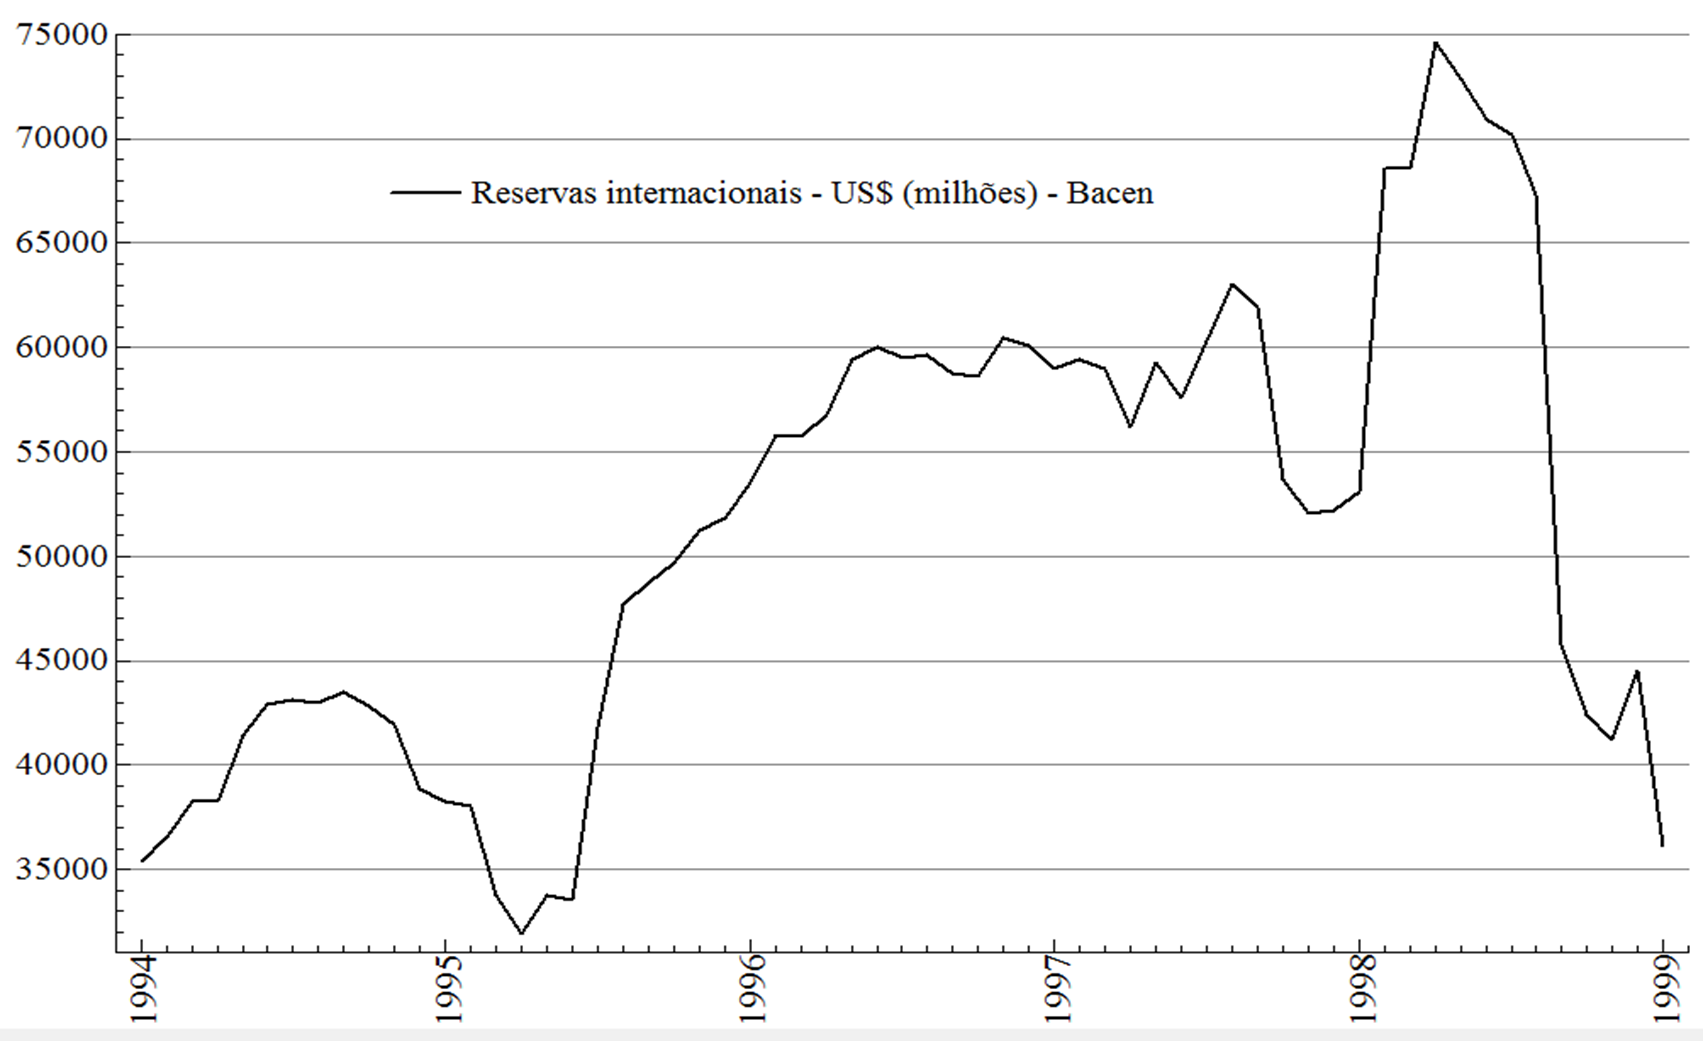
\includegraphics[width=0.7\linewidth]{Imagens/a14i2.png}
\end{figure}

Podemos ver que o Banco Central tinha o objetivo de trazer a inflação para patamares menores, com juros superiores as inflações. E os picos de taxa de juros coincidem com os momentos de declínio das reservas internacionais.

\begin{figure}[H]
    \centering
    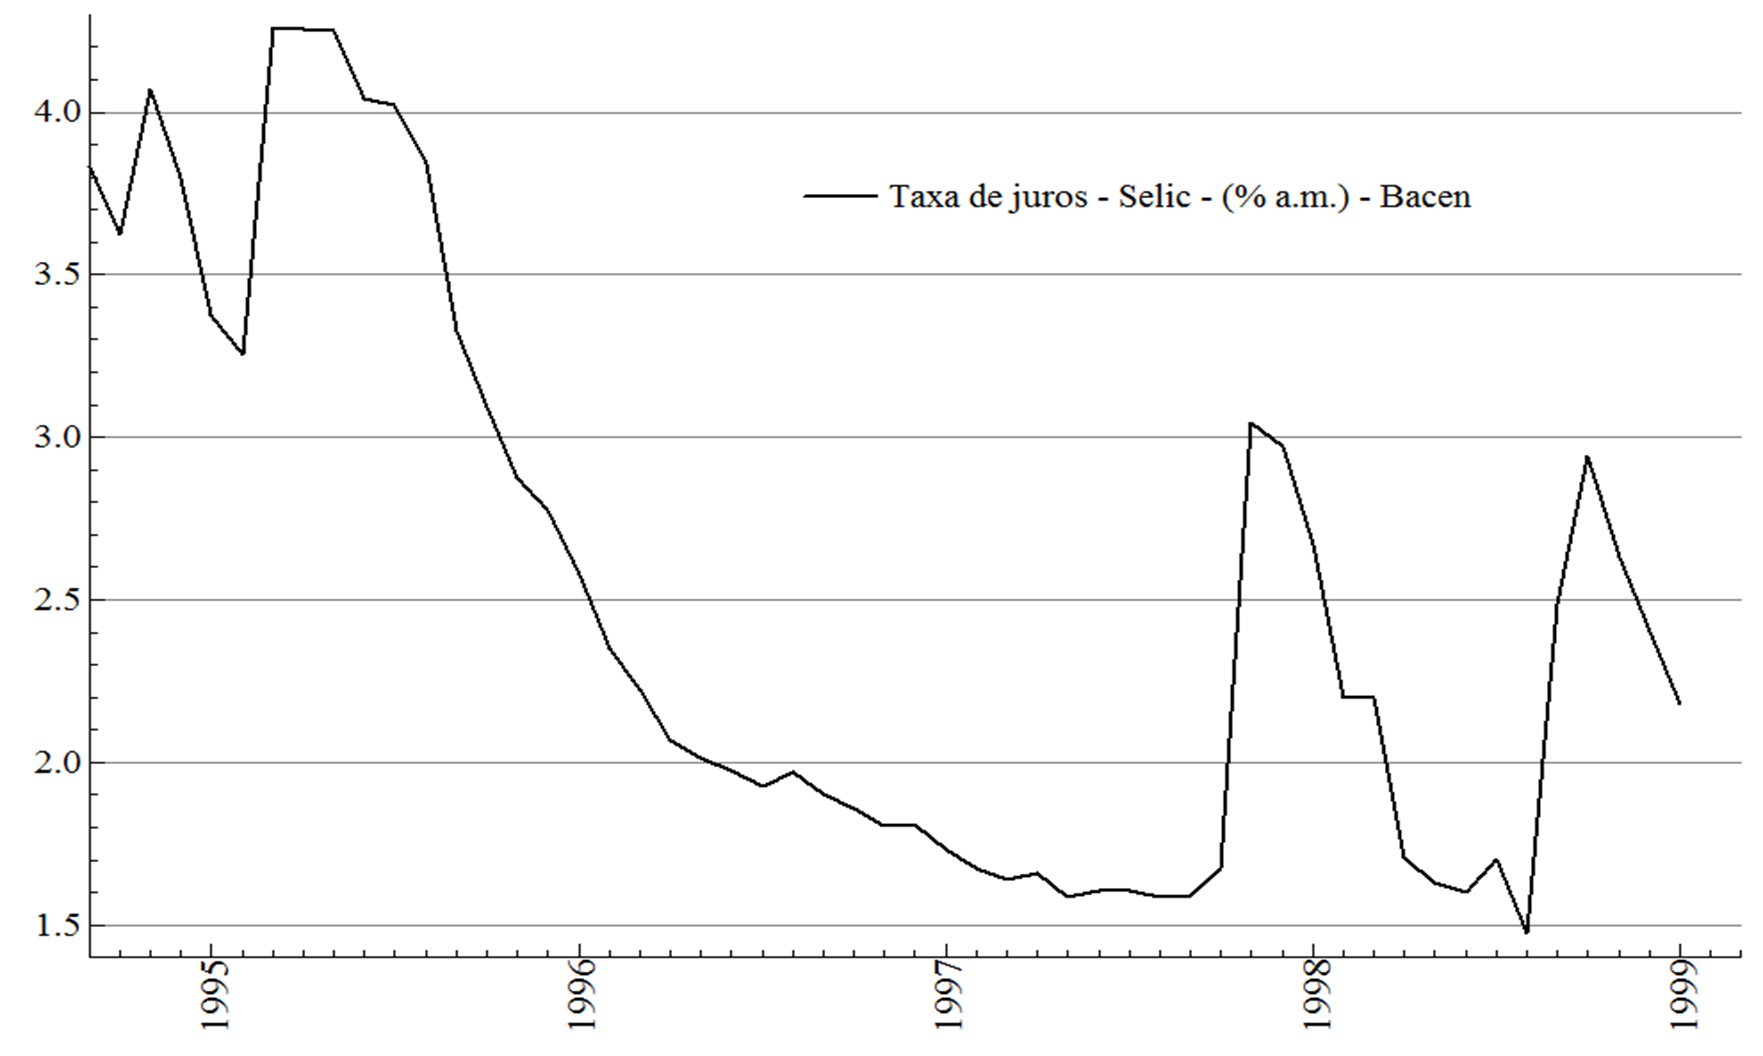
\includegraphics[width=0.7\linewidth]{Imagens/a14i3.png}
\end{figure}

\subsection{\textbf{Desequilíbrio externo}}
As transações correntes (TC) mudam(e muito): déficit de US\$2 bilhões em 1994 atinge um déficit 30 bi em 1997! Uma grande mudança. Isso é uma \textbf{PIORA} do BP, para entender isso temos que olhar a Balança Comercial(BC) e para a Balança de Serviços e Renda(BS/R). 

Qual é a dinâmica dessa deterioração?\begin{itemize}
    \item Significativa piora da BC em 1994(devido ao efeito riqueza e aumento das importações) e, consequente, piora das TC; O câmbio(que se valorizou) pode ser um motivo também para justificar a piora da BC , via câmbio real(Pastore mostrou isso via quatro medidas de câmbio real). E o FHC teve uma política fiscal expansionista, mais um possível motivo desse resultado. 
    \item O déficit em TC foi sendo saldado com a crescente entrada de capital estrangeiro(Conta de Capitais(CK); IED(investimento estrangeiro direto) acelera desde o início de 1995); Devido aos agentes "esperançosos" com melhoras no futuro do Brasil, com os juros altos brasileiros os investidores querem lucrar com isso. A CK vai nosso "financiador" da nossa conta corrente.
    \item Mas essa entrada gera, ao longo do tempo, impacto negativo sobre a BS/R com elevação dos compromissos com juros, de remessas de lucros e pagamentos de dividendos (devido aos agentes econômicos que colocaram dinheiro no Brasil;forte aumento desde o início de 1994). Provavelmente , esta foi o principal fator da pioro da nossa TC.
\end{itemize}

Assim, temos uma dinâmica que piorou o déficit em TC, visualmente podemos ter uma noção desses processos no gráfico abaixo:
\begin{figure}[H]
    \centering
    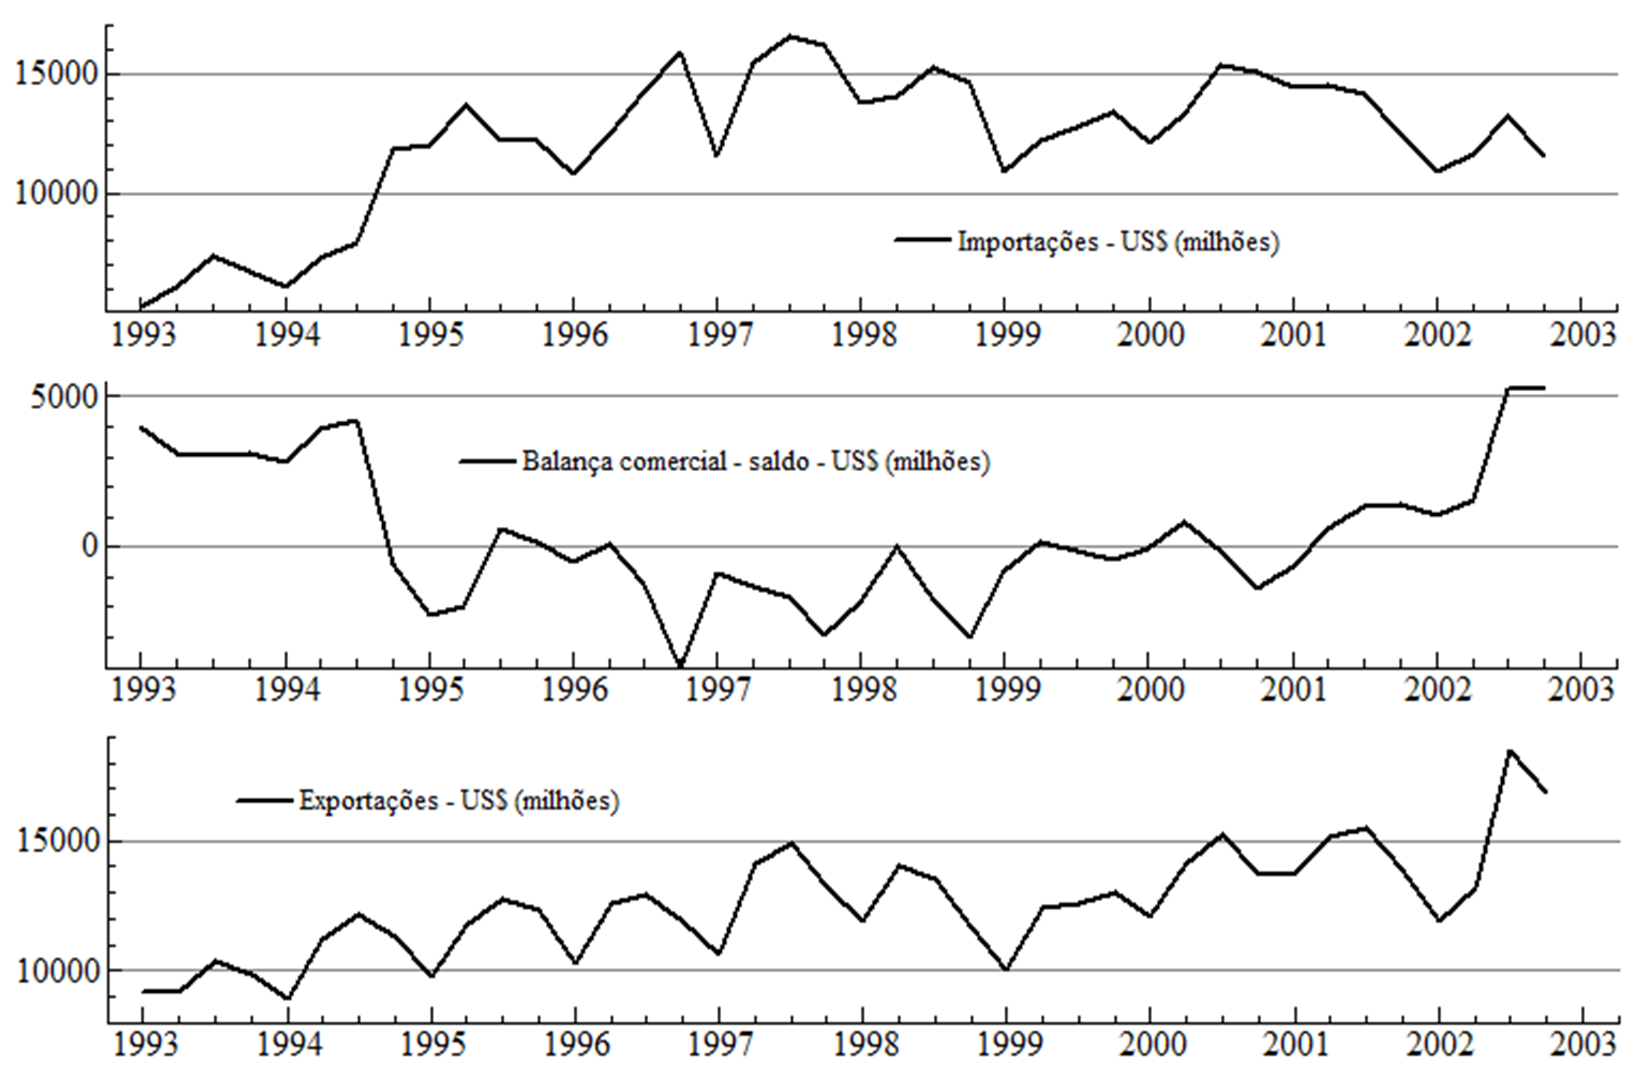
\includegraphics[width=0.7\linewidth]{Imagens/a14i4.png}
\end{figure}

Como explicar essa piora da TC?\begin{itemize}
    \item Com a estabilização dos preços, o consumo cresceu forte;
    \item A própria dinâmica, já que o financiamento ocorreu a partir da entrada de IDE e isto elevou o déficit de serviços e de rendas;
    \item Uma taxa de câmbio real apreciada, com desvalorizações muito pequenas ao longo do tempo;
    \item A política fiscal expansionista elevou a absorção, pressionando os déficits nas contas correntes.
\end{itemize}

Aqui vemos um outro lado, e complementar, dos motivos da piora da TC.

\begin{figure}[H]
    \centering
    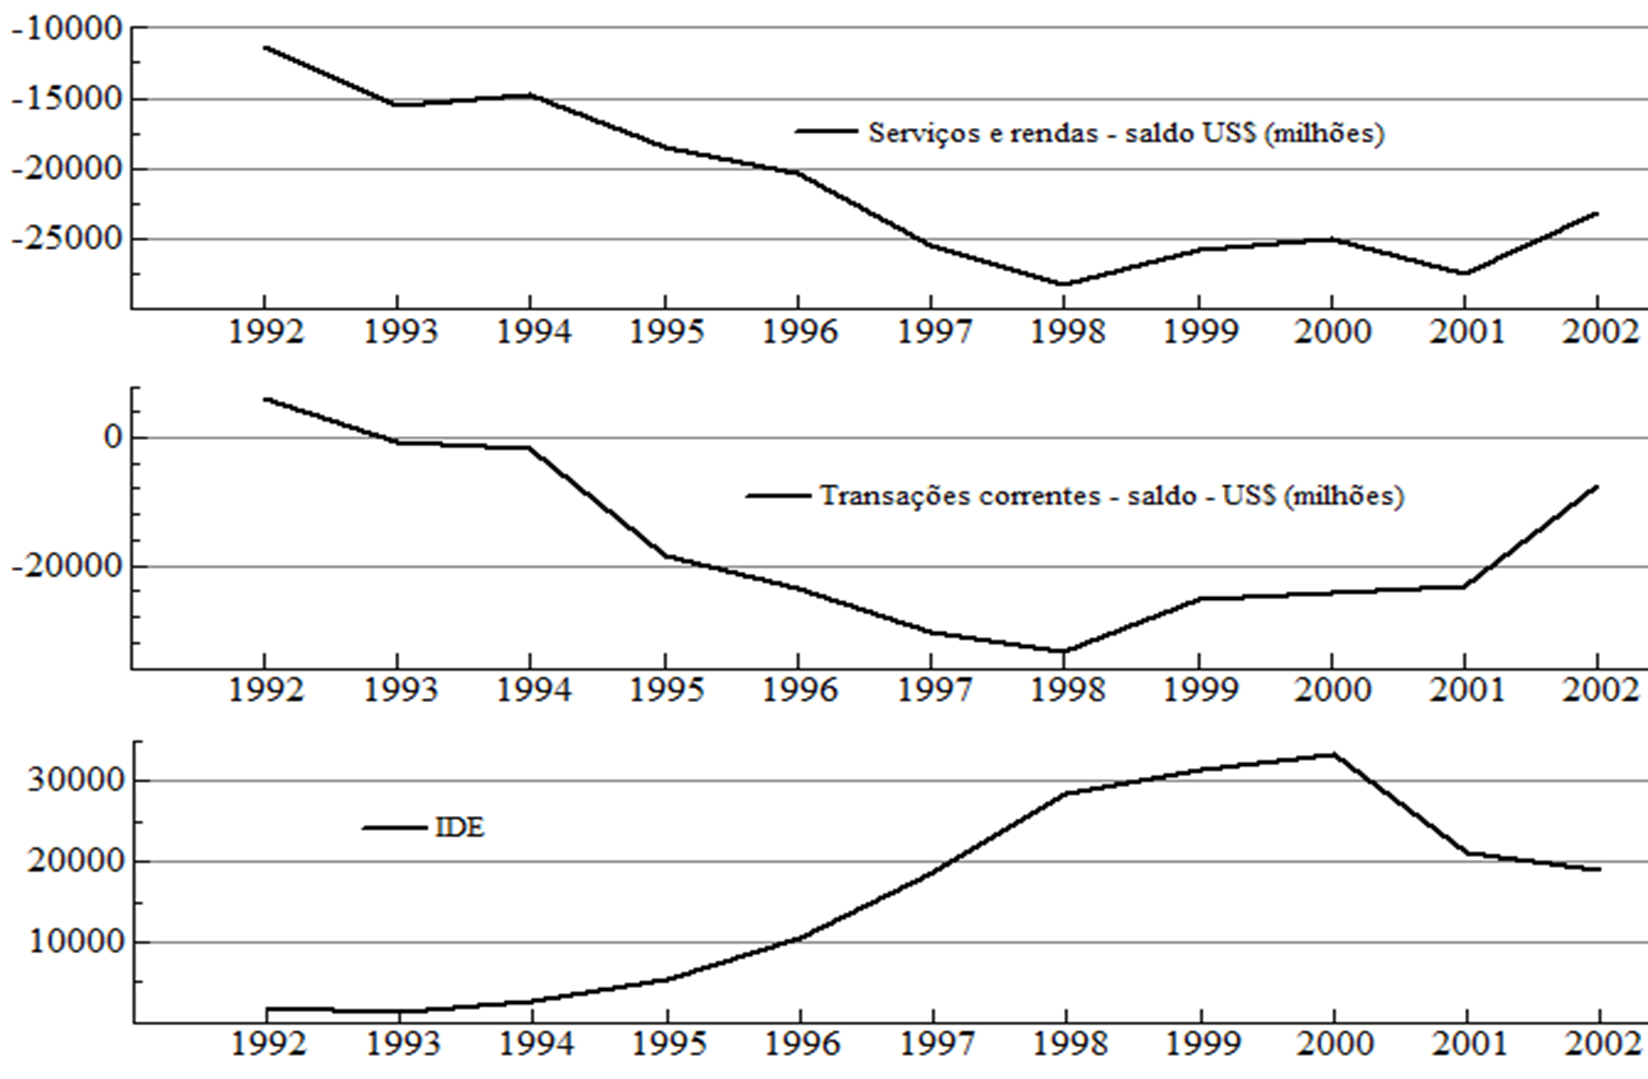
\includegraphics[width=0.7\linewidth]{Imagens/a14i5.png}
\end{figure}

\begin{figure}[H]
    \centering
    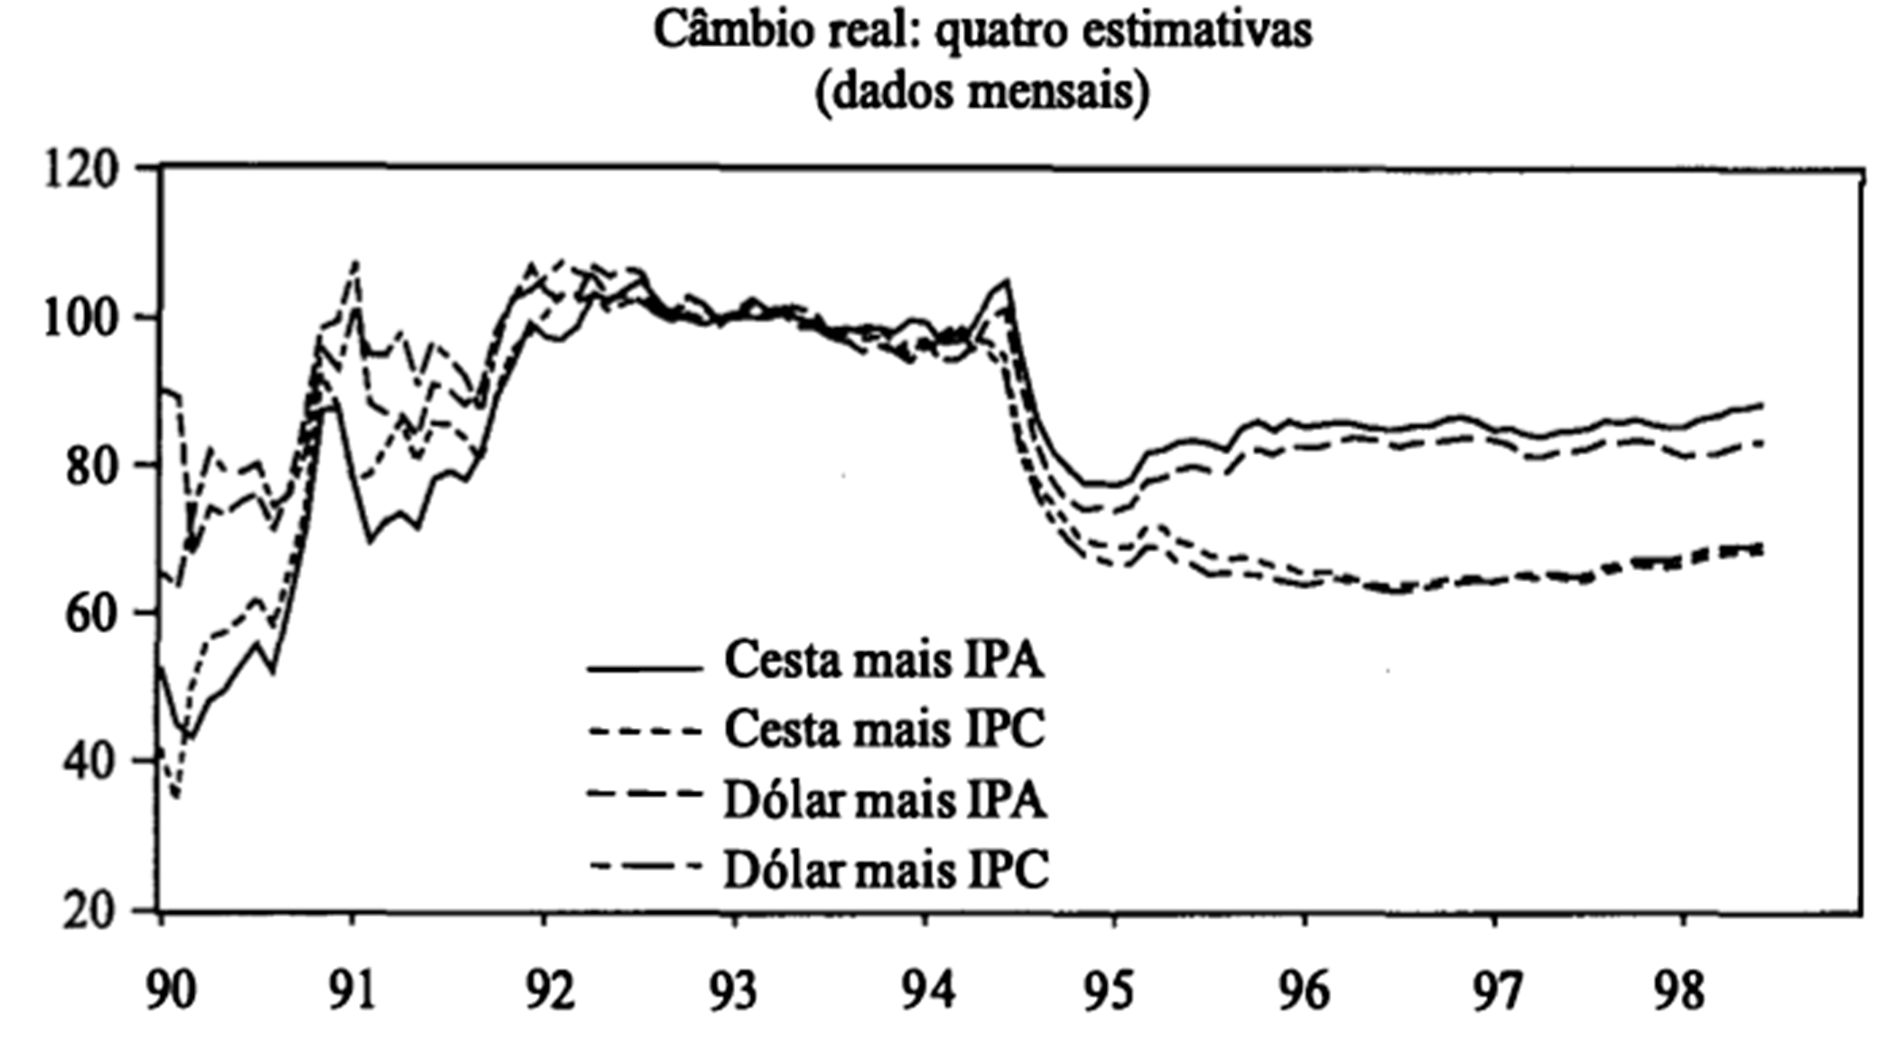
\includegraphics[width=0.7\linewidth]{Imagens/a14i6.png}
\end{figure}

\subsection{\textbf{Consolidar a estabilização e o setor externo}}

Lógica do governo: uma deterioração externa controlada seria melhor do que o retorno da aceleração da inflação

Houve medidas de contenção da demanda que em conjunto com medidas protecionistas deixaram a BC positiva (2º sem. 1995)

Houve queda do nível de atividade que reforçou a queda dos preços

O governo contava com um fluxo de capitais significativo

Mas, isso demandava taxas de juros elevadas\begin{itemize}
    \item foram crescentes, dados os “efeitos contágio” das crises externas;
    \item o que prejudica a recuperação do crescimento econômico;
    \item deixa o crescimento do PIB “errático”;
    \item piora a relação dívida pública/PIB.
\end{itemize}

\begin{figure}[H]
    \centering
    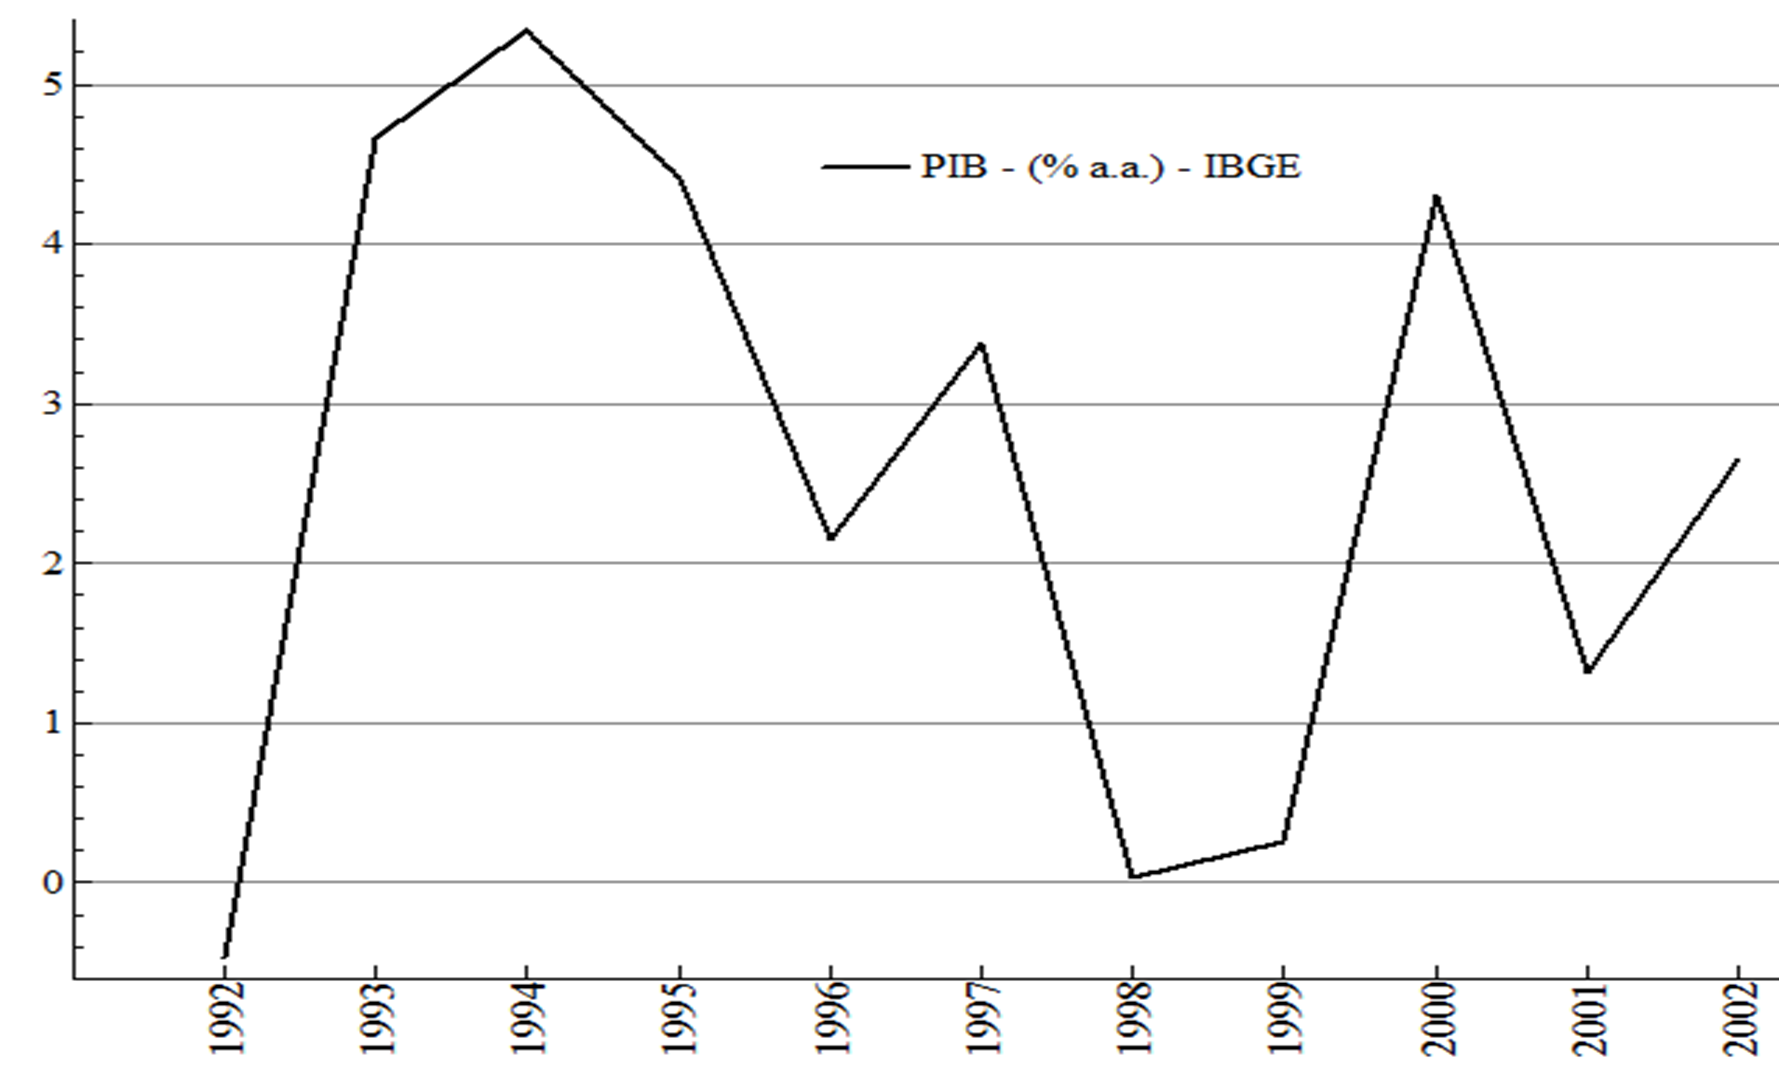
\includegraphics[width=0.7\linewidth]{Imagens/a14i7.png}
\end{figure}

\subsection{\textbf{Deterioração fiscal}}
Entre 1990 e 1994, os superávits primários oscilaram entre 1,6 e 5,2\% em relação ao PIB, transformaram-se em pequenos superávits ou déficits. 

Fim da inflação reduz o efeito “Tanzi às avessas” 

Inflação maior reduzia o déficit operacional, a queda da inflação mostrou o “verdadeiro” déficit (contribuição de Bacha)\begin{itemize}
    \item Senhoriagem, em relação ao PIB, declinou(Pastore demonstrou isso, apesar de ser difícil mostrar o valor da Senhoriagem, ele consegue mostrar isso)
    \item A 1ª fase do Real (fiscal) não foi completa
    \item Elevação dos juros trouxe aumento do déficit público 
    \item mas a piora do resultado primário pesou muito mais. Política fiscal foi expansionista em 1995! Isso explica os resultados. Mas porque ? FHC e sua equipe econômica queria limpar a sujeira dos governos anteriores nos planos de estabilização anteriores. "Esqueletos Fiscais", FHC achou esses esqueletos fiscais e quis dar um fim.
\end{itemize}

\begin{figure}[H]
    \centering
    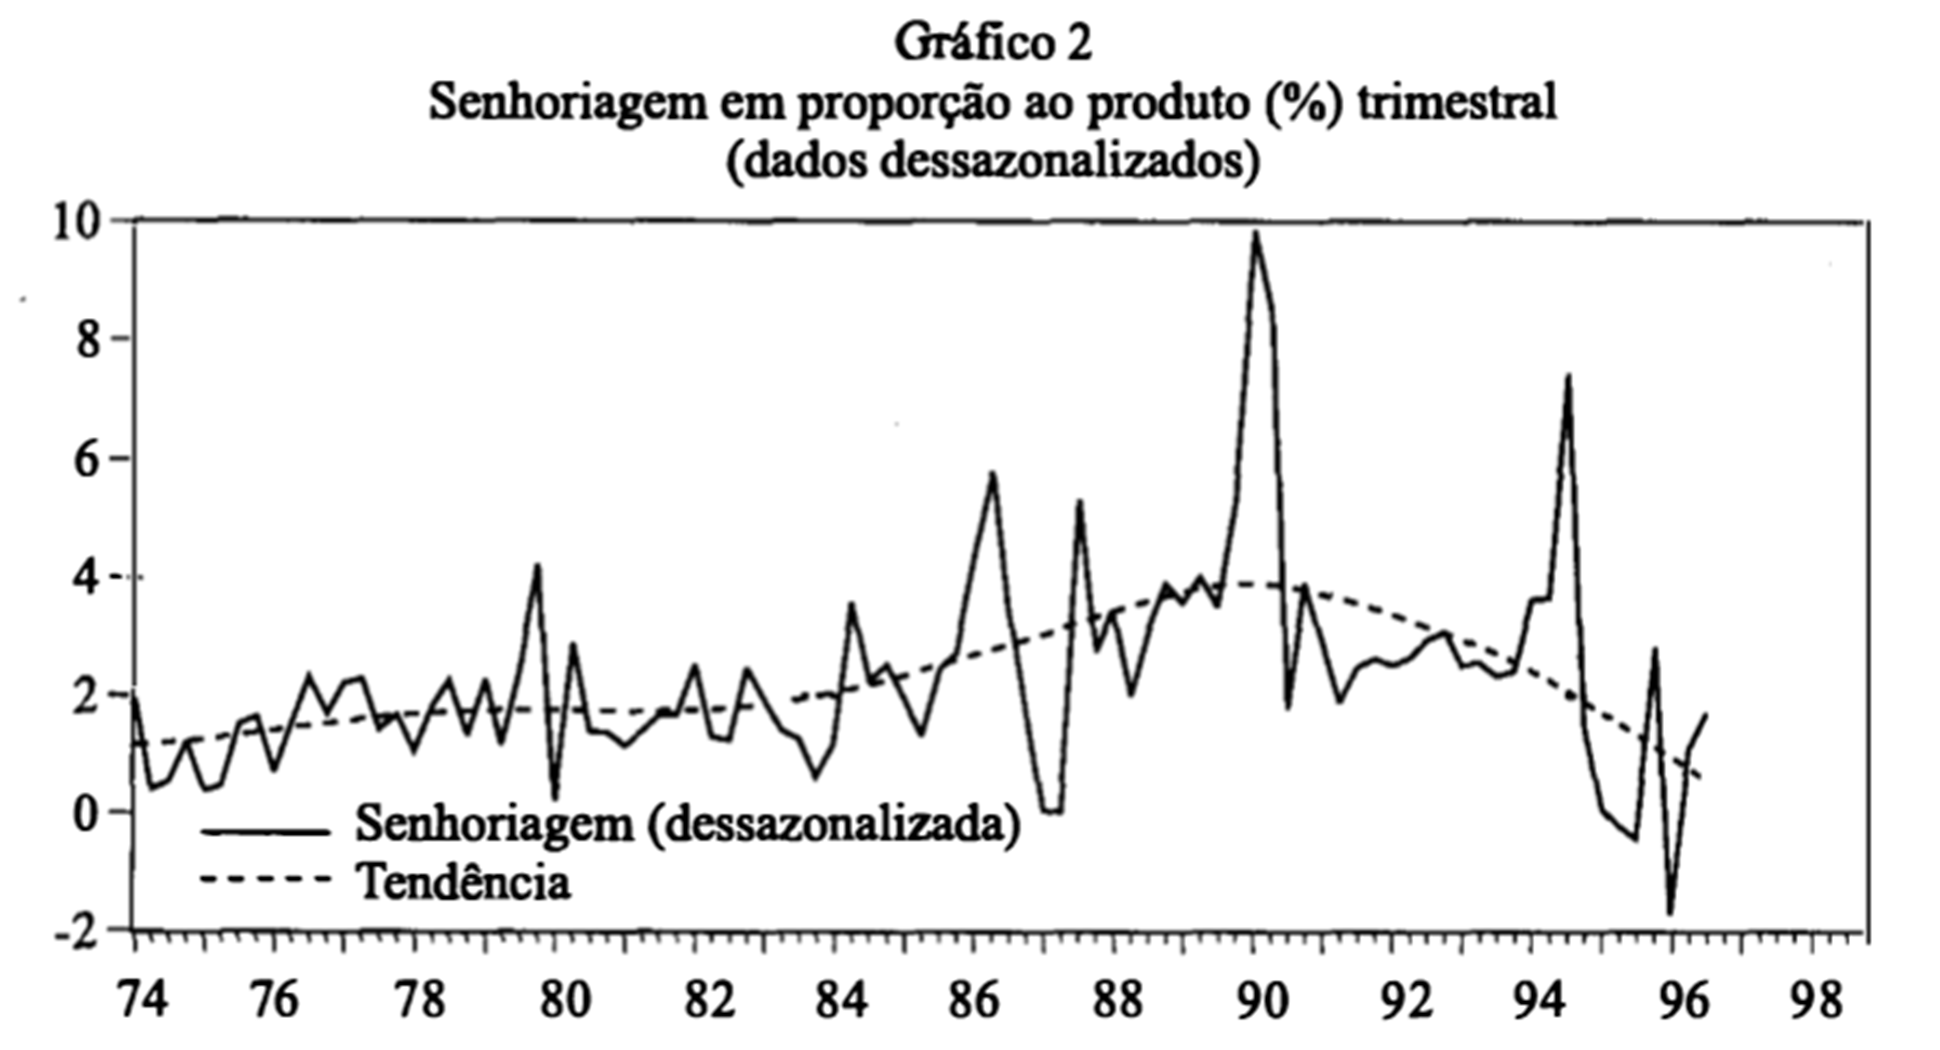
\includegraphics[width=0.7\linewidth]{Imagens/a14i8.png}
\end{figure}

\begin{figure}[H]
    \centering
    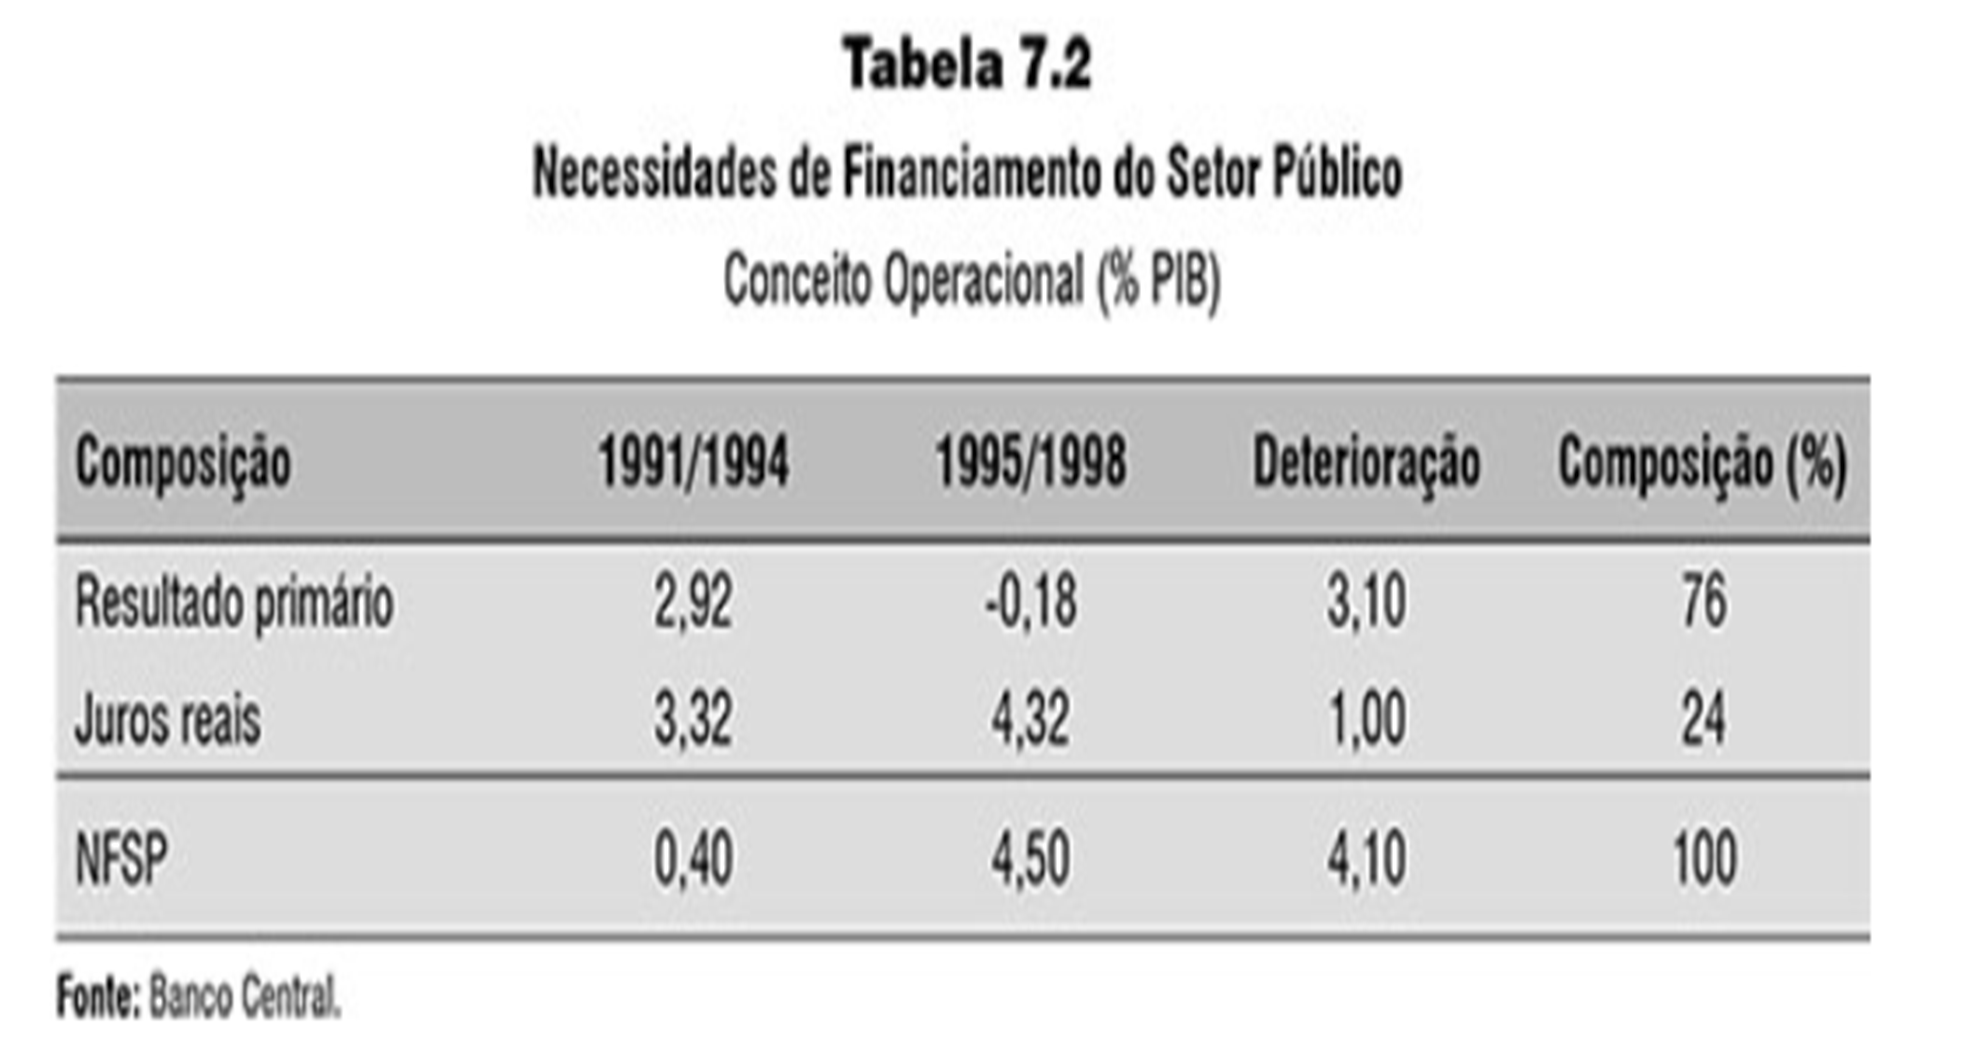
\includegraphics[width=0.7\linewidth]{Imagens/a14i9.png}
\end{figure}
\textbf{NFSP }: Necessidade de Financiamento do Setor Público

O sistema bancário exigiu intervenção (PROER; antes criticado hoje elogiado)\begin{itemize}
    \item Programa de Estímulo à Reestruturação e ao Fortalecimento do Sistema Financeiro Nacional, lançado em novembro de 1995; Exemplo foi o Banespa
    \item O fim da inflação reduziu fortemente os ganhos bancários (fim do \textbf{\textit{overnight}});
    \item O governo mencionava que sem essa intervenção, os sistemas bancário e financeiro poderiam colapsar;
    \item Auxiliou bancos privados e estaduais (“financiavam governadores”);
    \item O saneamento desses bancos viabilizaria processos de privatização e de fusões;
    \item Onerou significativamente os cofres do governo (R\$ 16 bilhões);
    \item Politicamente foi muito desgastante.
    \item Ideia do \textbf{PROER} era pegar os Bancos \textbf{Públicos e Privados} desestruturados, injetar capital para não gerar crises bancárias, subsidiar suas vendas para outras instituições bancárias de forma minimamente ajustada.
\end{itemize}

\subsection{\textbf{Privatizações no governo FHC}}
O cenário fiscal de 1995 exigiria forte reorganização em 1996. Medidas:\begin{itemize}
    \item Processo grande de privatizações de estatais e de empresas públicas, exemplo disso são a Vale do Rio Doce (Mineração) e o serviço de telecomunicação (um serviço que possuí um monopólio natural).
    \item Isto traria financiamento externo e reduziria pressão sobre a dívida de pública, atacando os dois desequilíbrios. A privatização, feita de maneira organizada e  bem regulada, pode tornar o serviço desse setor mais produtivo. Além disso, bons processos de privatizações, atraem capitais estrangeiros, isso atrai \textbf{IDE}, o que melhora a conta de capitais (\textbf{CK}), e os lucros das empresas privadas, podem levar a um fluxo de saída de dólares para a empresa matriz (\textbf{BS/R})  
    \item Mas esse processo também exigia forte apoio político e se mostrou lento
    \item Envolveu a criação de agências reguladoras e forte “conflito” com a antiga estrutura das empresas estatais, além de ser um órgão para a transição do público para o privado, mas também como uma garantidora do contrato exigido no momento de compra. E quanto mais transparente e eficiente seria essa agência reguladora, melhor seria esse momento de transição.
\end{itemize}

\begin{figure}[H]
    \centering
    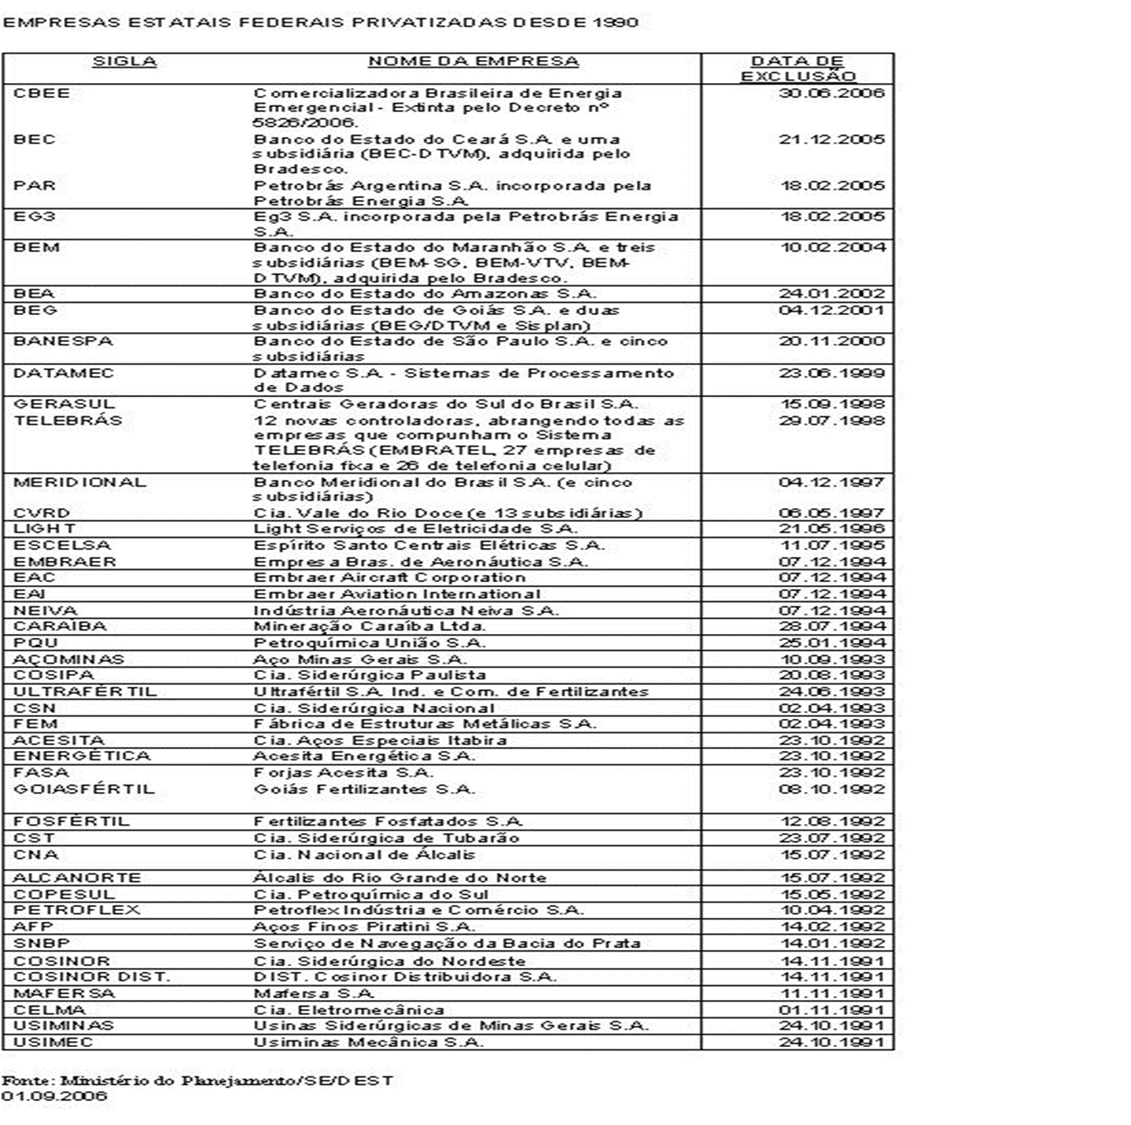
\includegraphics[width=0.7\linewidth]{Imagens/a14i10.png}
\end{figure}

\subsection{\textbf{Regimes cambiais e a política monetária}}
É difícil criar uma nova moeda e gerar uma estabilidade econômica, para isso o câmbio seria a ferramenta para essa âncora para a estabilidade. Um câmbio administrado, garante uma possível melhora do \textbf{BP}, devido a melhoria das \textbf{Reservas Internacionais}.

Entre junho e dezembro de 1994\begin{itemize}
    \item Câmbio flutuante sem intervenções do Bacen (isso é realmente um câmbio flutuante);
    \item Combinado com juros altos, o câmbio apreciou; O Brasil decidiu, por conta dos objetivos de frear a demanda por moeda e a demanda, além de querer atrair capital estrangeiro para aumentar as Reservas internacionais.
    \item Controle da quantidade de moeda era possível (no campo teórico, na prática não é possível).
\end{itemize}

Do início de 1995 até março\begin{itemize}
    \item Câmbio flutuante com intervenções do Bacen ("intervenção suja").
\end{itemize}

De março de 1995 em diante\begin{itemize}
    \item Flutuante com intervenções do BACEN, seguindo uma correção pré-fixada (micro desvalorizações com “minibandas”); A autoridade cambial brasileira (BC) montou isso dessa forma para mostrar que o Real (a nova moeda) é tão estável quanto o dólar.
    \item Oferta monetária torna-se passiva (BC sem controle da política monetária), diante da mobilidade de capitais.
\end{itemize}

\begin{figure}[H]
    \centering
    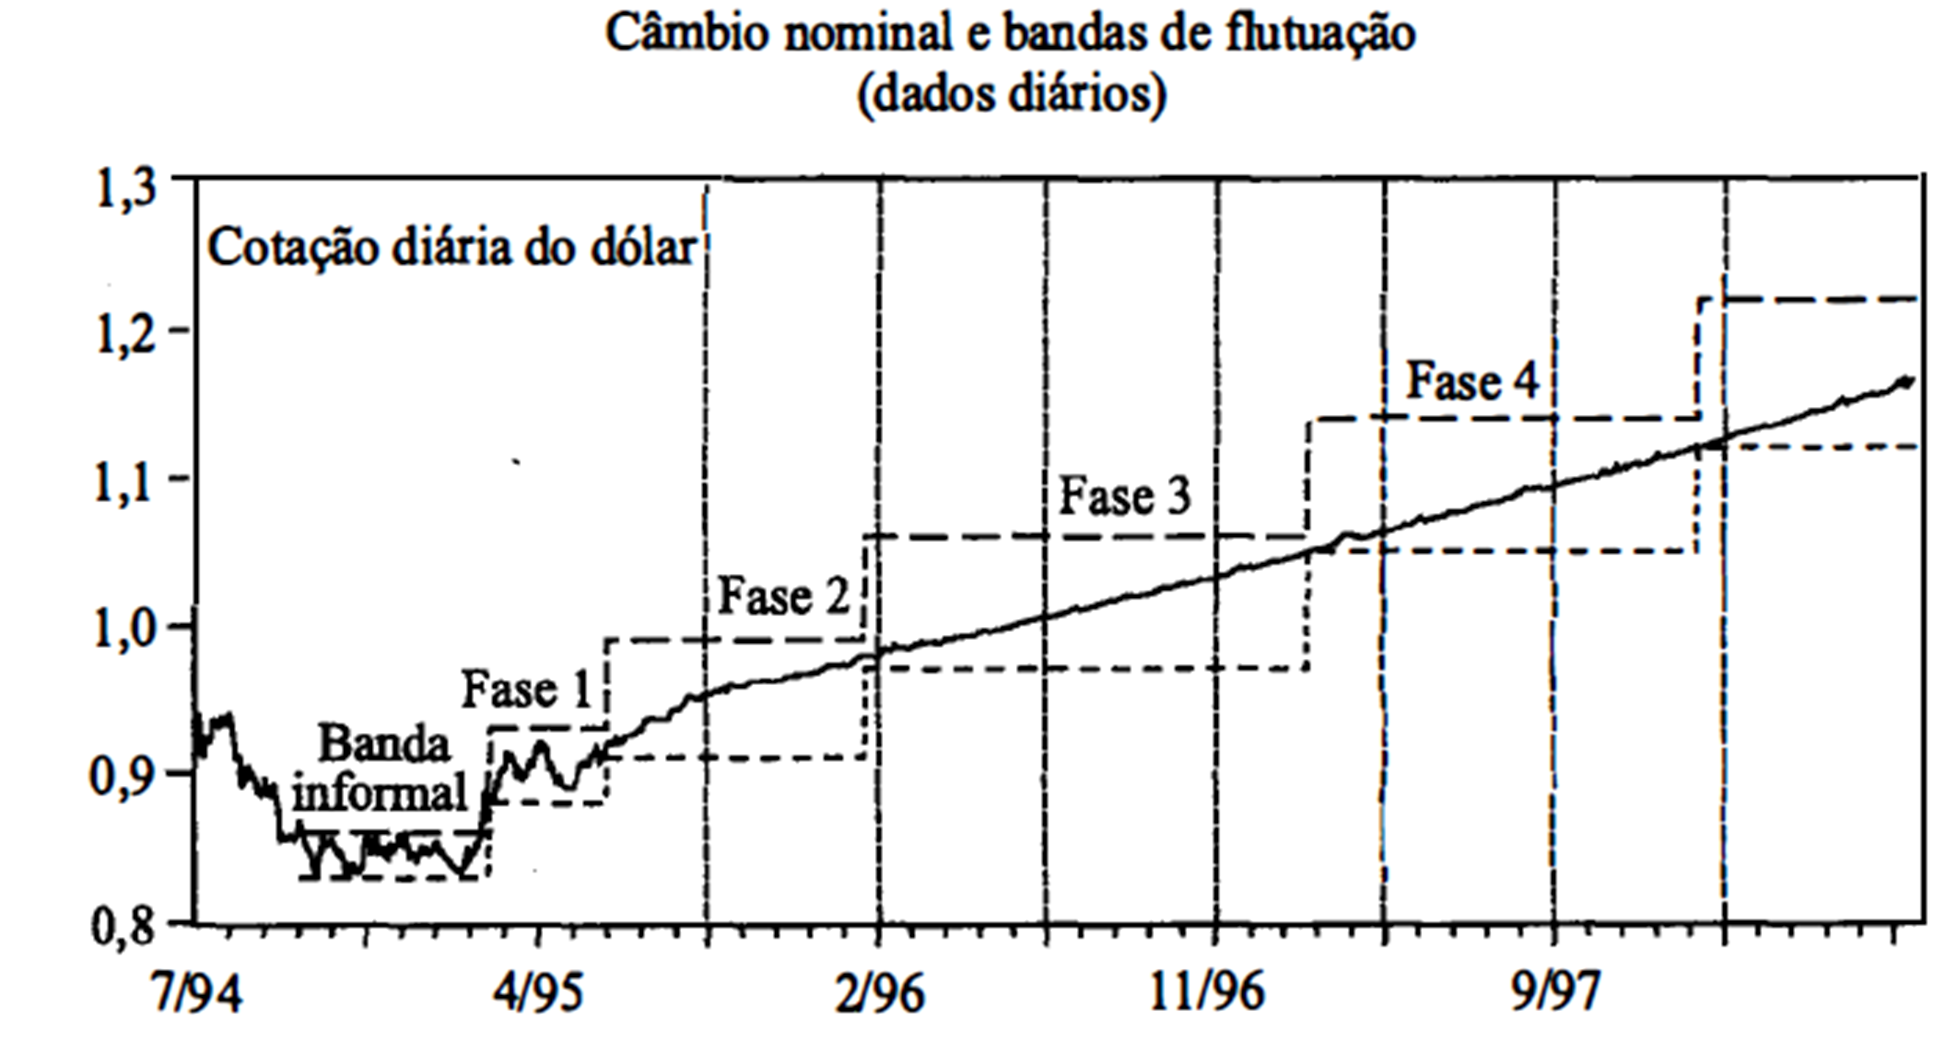
\includegraphics[width=0.7\linewidth]{Imagens/a14i11.png}
\end{figure}

\textbf{Sistema de Pré-fixação da Taxa de Câmbio}(\textit{Pastore}):É nítido o quão estreito era as bandas cambias eram estreitas e seu processo de desvalorização era contínuo. Porém era algo escalonado e controlado. Em quase 4 anos, o câmbio desvalorizou \(\approx 17,39\%\). Isso mostra, através da âncora  cambial, mostra o quanto o Real é equiparável ao dólar. Além de garantir uma estabilidade econômica, visto as crises ao longo desses anos e as baixíssimas variações frente as fugas de capitais.

\subsection{\textbf{Por que a opção inicial de flutuação cambial?}}

No contexto de juros altos, geraria apreciação o que ajudaria a consolidar a estabilização de preços (importante para credibilidade do Plano Real)\begin{itemize}
    \item Era importante na visão de Gustavo Franco;
    \item Os déficits nas contas correntes poderiam ser financiados com entradas de capitais (havia espaço para valorizar o câmbio real);
    \item Mas isso foi frustrado, pois a combinação entre valorização cambial, liberalização comercial e forte crescimento do consumo gerou déficits nas contas correntes “acima do moderado”.
\end{itemize}

\subsection{\textbf{As crises financeiras internacionais (1994-1998)}}
O Brasil escolheu defender o regime cambial no período 1995/98\begin{itemize}
    \item Seria importante neste contexto avaliar os riscos que envolviam o setor externo brasileiro;
    \item Diante de seguidas crises externas, a política monetária foi direcionada para promover o equilíbrio do setor externo;
    \item Havia efeitos colaterais: conviver com recessão e aceitar o aumento do déficit público. 
\end{itemize}

\begin{figure}[H]
    \centering
    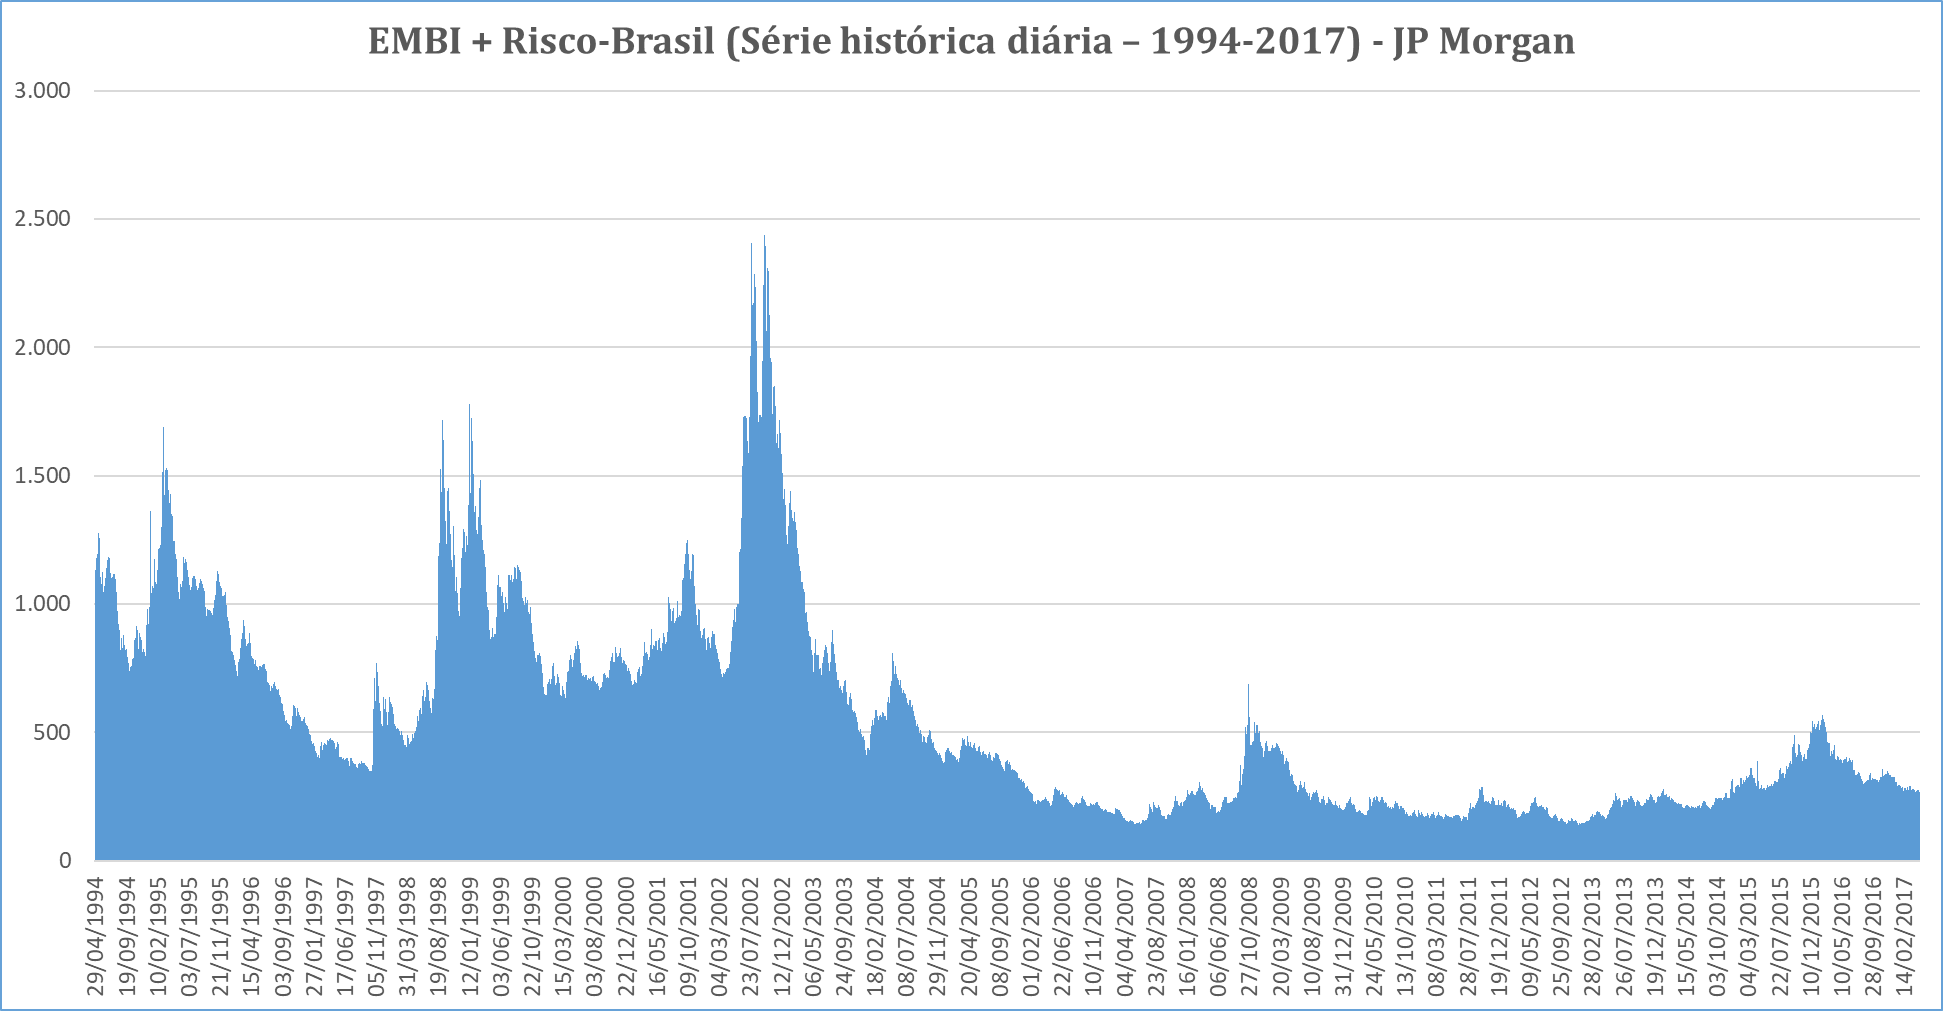
\includegraphics[width=0.7\linewidth]{Imagens/a15i1.png}
\end{figure}

\begin{figure}[H]
    \centering
    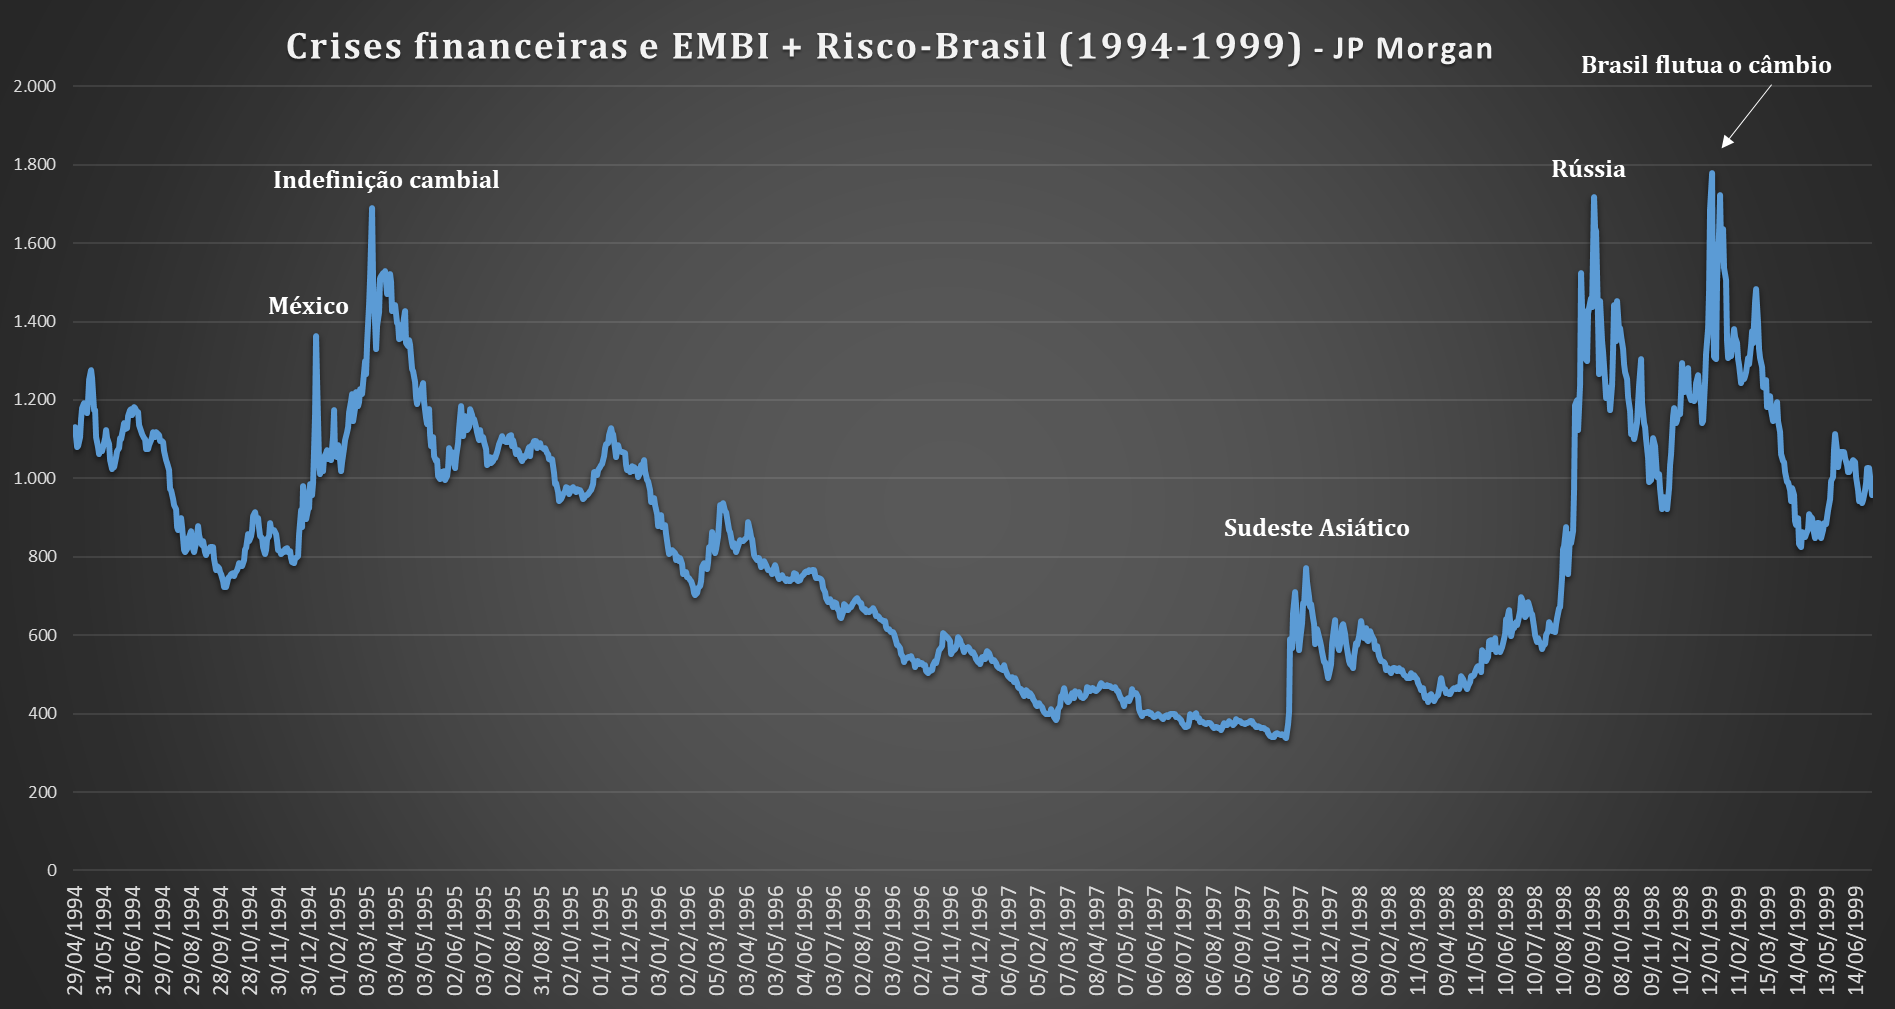
\includegraphics[width=0.7\linewidth]{Imagens/a15i2.png}
\end{figure}

\subsection{\textbf{Reação à crise mexicana (dez1994/jan1995)}}

Ao final de 1994 a crise mexicana coincide com o pico do aquecimento do consumo

Governo adota política monetária fortemente contracionista\begin{itemize}
    \item eleva compulsório (e reduz prazo máximo de empréstimos);
    \item juros do crédito ao consumidor praticamente dobram;
    \item eleva as taxas de juros (Selic vai de 9\% aa para 35\%!);
    \item a opção foi seguir bandas a partir de taxas de compra e venda divulgadas ao mercado.
\end{itemize}

Houve certa indefinição na adoção do sistema “crawling-peg”, gerando volatilidade no ingresso de capitais (o câmbio seria desvalorizado? Descontroladamente?)\begin{itemize}
    \item isto provocou perda de reservas superior ao próprio momento da crise mexicana
\end{itemize}

Medidas e efeitos\begin{itemize}
    \item o governo liberalizou mais o ingresso de capitais estrangeiros;
    \item reduziu o IOF sobre operações financeiras com moedas estrangeiras;
    \item a crise cambial foi controlada e os fluxos de capitais revertidos;
    \item queda do produto industrial, inadimplência e custo da dívida cresceram com os juros elevados.
\end{itemize}

\subsection{\textbf{Reação à crise do Sudeste Asiático (1997)}}

Em outubro de 1997 cresceu o risco Brasil

O governo decidiu preservar o sistema cambial e, para isso, elevou as taxas de juros\begin{itemize}
    \item Isso desaquecia a economia, o que tendia a reduzir os déficits comerciais
    \item Estimulava entrada de capitais (ou menor saída), estabilizando as reservas internacionais
    \item Houve saídas de reservas em out/nov, mas estabilizaram em dezembro
    \item Produção industrial mostrou forte queda ao final de 1997
\end{itemize}

Para preservar o sistema cambial, a velocidade da queda de juros brasileira seria função:\begin{itemize}
    \item de conseguir preservar suas reservas internacionais
\end{itemize}

Mas:\begin{itemize}
    \item Teria de conviver com uma recessão profunda;
    \item E com um impacto forte no déficit público;
\end{itemize}

Isso quer dizer: a política monetária do Bacen estava buscando equilíbrio do setor externo.

\subsection{\textbf{Reação à crise Russa}}
A combinação de forte mobilidade internacional de capitais com regime de câmbio fixo iniciou as crises mexicana e asiática

Essa combinação contribuiu para a Rússia entrar em crise, que ainda apresentava um grave problema fiscal e baixa capacidade de arrecadar impostos

Como o FMI “salvou” os envolvidos nas crises anteriores, isso estimulou grande fluxo de capitais, testando a solvência russa

Resultado: para enfrentar sua crise fiscal, a Rússia usou a opção do default da dívida interna e externa, impondo fortes perdas aos investidores

Ocorre que após ter enfrentado as duas crises anteriores, a força da política econômica brasileira perde eficácia

Os riscos dos mercados emergentes foram crescentes desde maio de 1998 (a crise Russa fica mais grave em agosto de 1998)\begin{itemize}
    \item Reduziram os fluxos de capitais para o Brasil; 
    \item Déficit público havia aumentado muito e os efeitos recessivos recorrentes desgastaram a prática da elevação dos juros;
    \item Por outro lado, a proximidade com as eleições e a chance da reeleição de FHC geraram certa paralisia e atraso para rever o regime cambial.
\end{itemize}

Um pacote de auxílio com o FMI não foi suficiente para evitar um novo ataque especulativo contra o Real\begin{itemize}
    \item Após alguns dias de tentativa de realizar uma desvalorização cambial controlada, o governo permitiu a flutuação do câmbio em janeiro de 99
\end{itemize}

\begin{figure}[H]
    \centering
    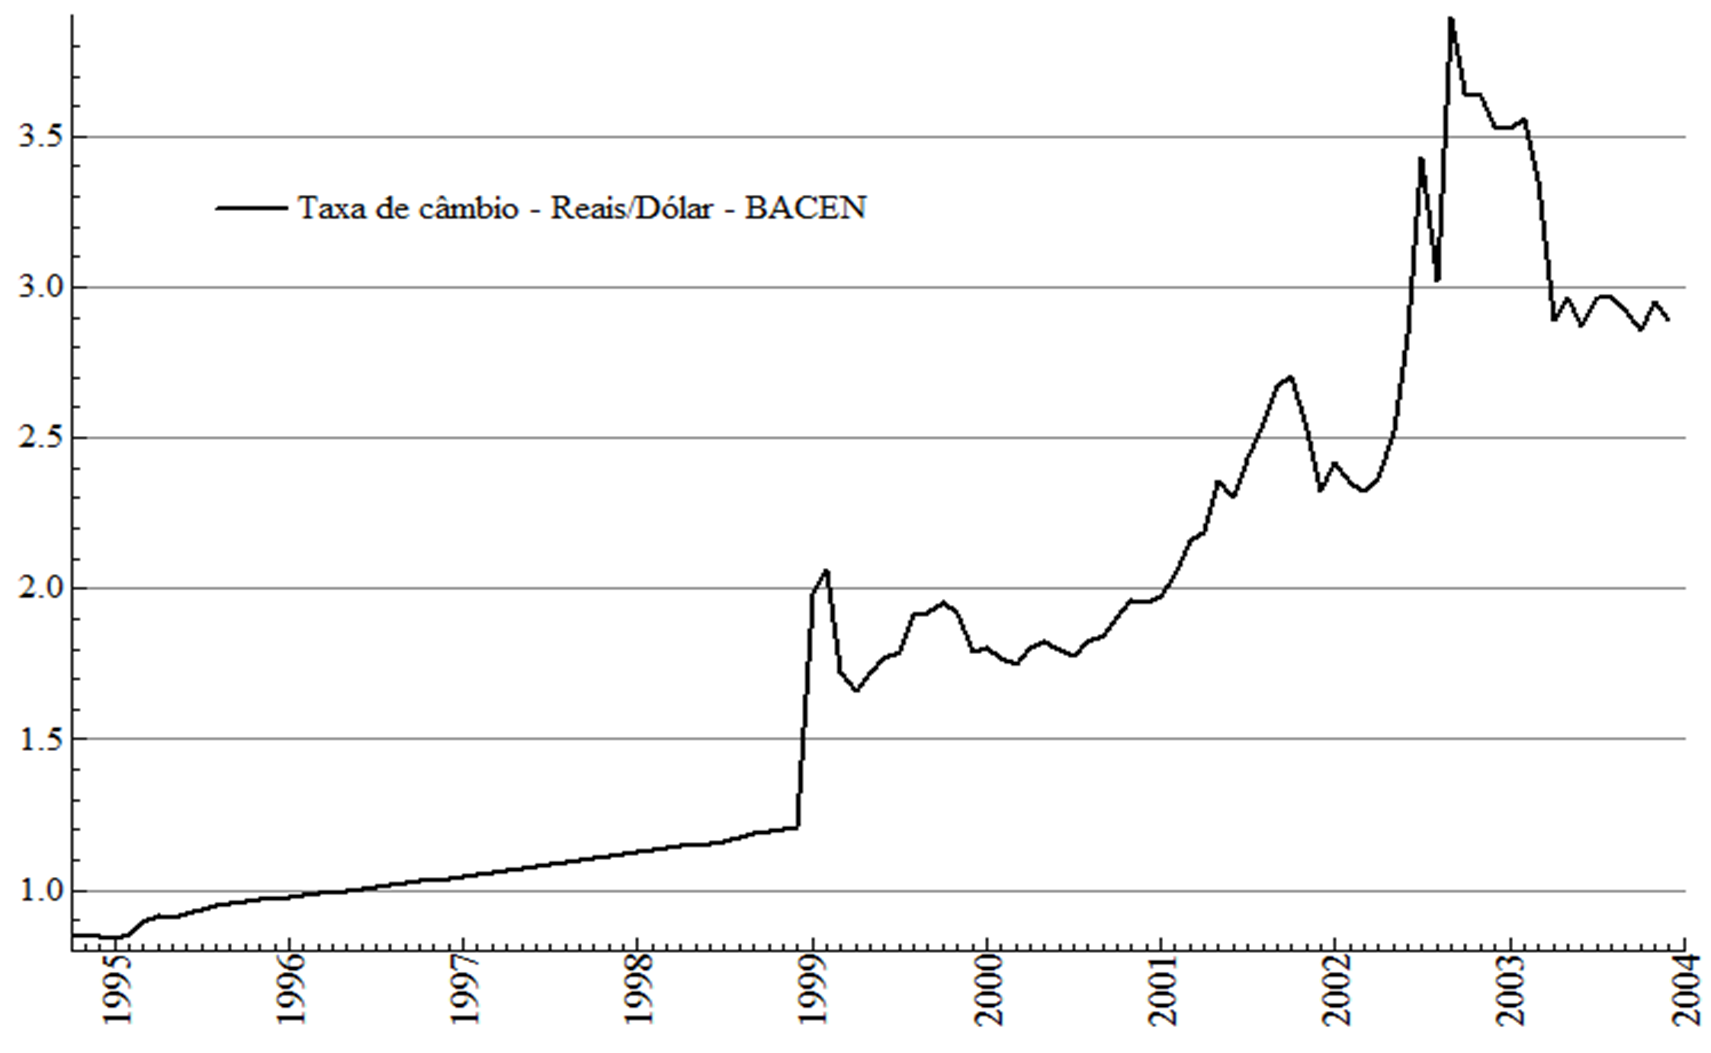
\includegraphics[width=0.7\linewidth]{Imagens/a15i3.png}
\end{figure}

\subsection{\textbf{O câmbio “apreciado”}}

A economia brasileira esteve exposta aos “efeitos contágio” dos choques externos\begin{itemize}
    \item Ocorreram vários (México, Ásia, Rússia e o próprio Brasil)
    \item Os custos envolvidos eram altos (expectativa de desvalorização do real, perda de reservas internacionais e grandes elevações de taxa de juros)
    \item A política fiscal expansionista elevou a absorção, pressionando os déficits nas contas correntes
\end{itemize}

\subsection{\textbf{Por que manter o câmbio apreciado?}}
Contribuição de G. Franco para consolidar a estabilização;

Mas, provavelmente a persistência nesta estratégia foi muito alta;

Houve muito desgaste (político e econômico);

Consenso: flutuação iria ocorrer “cedo ou tarde” e isso foi testado ao longo do tempo, deixando maior os custos de manter o controle;

Ficou mais arriscado ainda quando o Brasil voltou a crescer;
Mas preservar a queda da inflação seria vital para a reeleição.

\subsection{\textbf{Taxas de juros elevadas: uma necessidade?}}
Contribuição de Pérsio Arida e a importância da taxa de juros para a consolidação da estabilização (evitar explosão de consumo)

Contribuição de Gustavo Franco e a importância de taxa de juros para a consolidação da estabilização (fortalecer o controle cambial, importância de reservas internacionais também elevadas e setor externo equilibrado)

Reduziam o excesso de absorção provocada pela política fiscal expansionista, buscando pressionar menos os déficits nas contas correntes

Resultados: elevação do custo da dívida pública e crescimento econômico comprometido

\subsection{\textbf{O pós crise cambial}}

O problema cambial e a reeleição de FHC em 1º turno viabilizaram\begin{itemize}
    \item Ajuste fiscal significativo (ampliação da arrecadação e aprovação da Lei de Responsabilidade Fiscal)
    \item Remontagem institucional da lógica da política econômica\begin{itemize}
        \item Estabelecidas metas de superávit primário
        \item Implementado o regime de metas de inflação
        \item Adoção do regime cambial flutuante
    \end{itemize}
    \item Mas houve custos e perda de crescimento econômico
    \item Esse contexto foi agravado pela imposição de um racionamento de energia (2001)
\end{itemize}

\subsection{\textbf{Primeiros meses de 1999}}
FHC, tentando encurtar a crise manteve a equipe econômica.

Depois de um período de instabilidade, Armínio Fraga é nomeado no início de março, presidente do Bacen.

Renegociação com o FMI foi aberta (a crise tinha travado a negociação)

Os juros tinham sido elevados a 45\% e em conjunto a crise cambial deixava a situação da dinâmica da dívida muito grave (a dívida era de boa parte em títulos vinculados ao câmbio). Seria necessário um ajuste fiscal sério. Assim, os objetivos foram definidos:\begin{itemize}
    \item Equacionar o quadro fiscal
    \item Assegurar equilíbrio do setor externo
    \item Evitar que o choque cambial trouxesse descontrole inflacionário
\end{itemize}

\subsection{\textbf{O regime de metas de inflação (1999)}}

A partir da divulgação da meta, o CMN sinaliza como será a condução da política monetária. O dia a dia das reuniões do COPOM tenderá a:\begin{itemize}
    \item sinalizar aumentos dos juros caso a expectativa da inflação se desloque da meta. 
    \item O Bacen poderia, então, reduzir os juros se a expectativa fosse inferior à meta.
\end{itemize}

Na prática, é atribuído a este sistema um conjunto solucionador da crise cambial de 1999.

Em conjunto com o ajuste fiscal permitiu avaliações positivas da dívida e do menor impacto inflacionário, incentivando o ingresso de capitais:\begin{itemize}
    \item o câmbio apreciou
\end{itemize}

Deu à tona um discurso mais coerente para o contexto econômico de FHC: responsabilidade fiscal, câmbio flutuante e regime de metas de inflação. Esse contexto foi a tônica para explicar o ciclo econômico brasileiro virtuoso vivenciado pós março de 99.

\subsection{\textbf{Os anos 2000 e 2001}}
Em 2000 o contexto econômico havia sido ajustado:\begin{itemize}
    \item inflação estava sob controle (meta de 6\% seria cumprida) 
    \item havia um programa de consolidação fiscal (resultado primário de déficit de 1\% do PIB em 1997 mostrava superávit de 3,3\%!)
    \item dada a dificuldade política, boa parte desse ajuste tinha origem na criação de impostos
    \item por outro lado aprovou no Congresso a Lei de Resp. Fiscal
    \item a recuperação foi lenta da BC, mas a entrada de capitais melhorava o setor externo
    \item a economia voltou a crescer, anotando 4,3\% em 2000
    \item havia uma onda otimista dos empresários e agentes em geral, no sentido de que FHC faria seu sucessor e a transição seria suave. Mas.....
\end{itemize}

Ocorreram duas crises: Argentina e a energética\begin{itemize}
    \item Contexto externo não foi benéfico: houve forte crise da Argentina, atentados terroristas das torres gêmeas, queda médias nos preços das exportações brasileiras. 
    \item Em abril, o governo se deu conta que em decorrência da má gestão, o setor de energia elétrica apresentava excesso de demanda e o governo foi obrigado a fazer racionamento.
    \item Isso na prática levou a um grau maior de desvalorização o que desfavoreceu a relação preços e juros no sentido de dinamizar o crescimento econômico 
    \item foi evitada maior inflação (\(\uparrow\)juros) e houve queda dos salários reais decorrente da desvalorização. (trazendo dúvidas até em relação à dinâmica da dívida). Mas ao final de 2001 as piores previsões ficaram marginais.
\end{itemize}

\newpage
\section{\textbf{Problemas econômicos e política econômica(O período Lula 2003-2010)}}
\subsection{\textbf{Introdução}}
Tema
\begin{itemize}
    \item O PT e a ``Carta aos brasileiros''. A lógica econômica no primeiro governo Lula.
    \item O ``PT volta a ser PT''? A mudança da agenda econômica no segundo governo Lula.
\end{itemize}

O que é importante?
\begin{itemize}
    \item Entender as diferentes escolhas de política econômica nos governos Lula 1 e 2 e, a partir delas, quais foram as consequências.
\end{itemize}

Leitura: \textit{Ordem do Progresso} (Cap. 17) e \textit{Economia Brasileira Contemporânea} (Cap. 8)

\subsection{\textbf{Contexto em 2002}}
A probabilidade da vitória do PT nas eleições passa a ser alta e uma série de dúvidas são levantadas acerca da política econômica futura:

\begin{itemize}
    \item O governo FHC havia consolidado o discurso, combinando: responsabilidade fiscal, metas de inflação e câmbio flutuante;
    \item A linha de pensamento econômico no PT tinha, em grande parte, severas críticas a esse discurso, chegando a propor um plebiscito acerca do pagamento das dívidas externa e interna; Isso gerou uma dúvida em relação se o \textbf{Tripé Macro}, construído pelo governo FHC iria ser desfeito pelo possível governo do PT
    \item Alguns analistas cogitavam a possibilidade de moratória e de práticas populistas;
    \item Em menos de dois meses a Selic foi elevada de 18\% a.a. para 25\%;
    \item A medida de risco e a taxa de câmbio ilustram o cenário de dúvidas.
\end{itemize}

\begin{figure}[H]
    \centering
    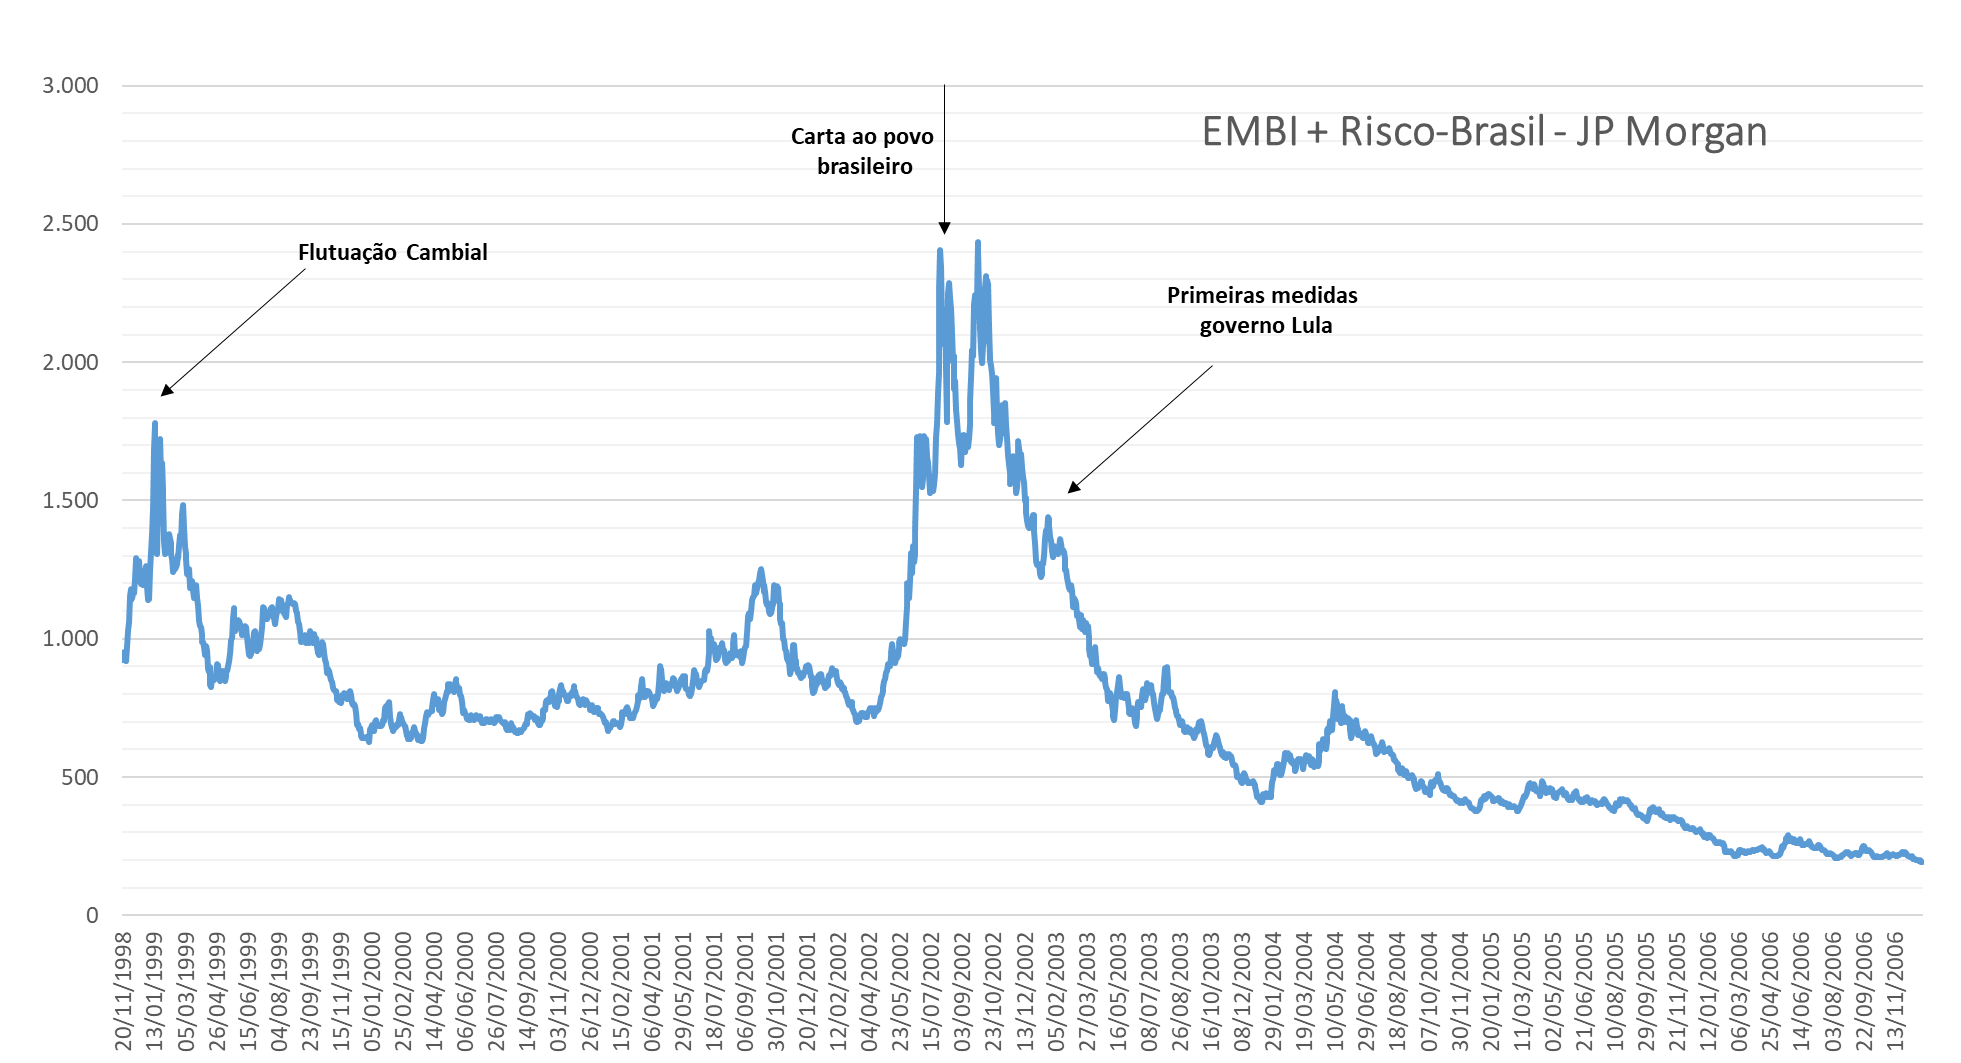
\includegraphics[width=0.7\linewidth]{Imagens/a16i1.png}
\end{figure}

Ajustando o câmbio dessa época para valores de hoje, seria um câmbio de quase R\$8 para 1 U\$, mostrando um desconfiança dos agentes econômicos em relação a futura administração do PT. Essa fuga de capitais para uma moeda mais "forte", também gerou uma incerteza inflacionária, o que exigiu uma aumento de juros longos, consequentemente, uma piora do cenários fiscal brasileira desde a estabilização econômica/inflacionária. Algo que pode ser tornar um ciclo vicioso.

\begin{figure}[H]
    \centering
    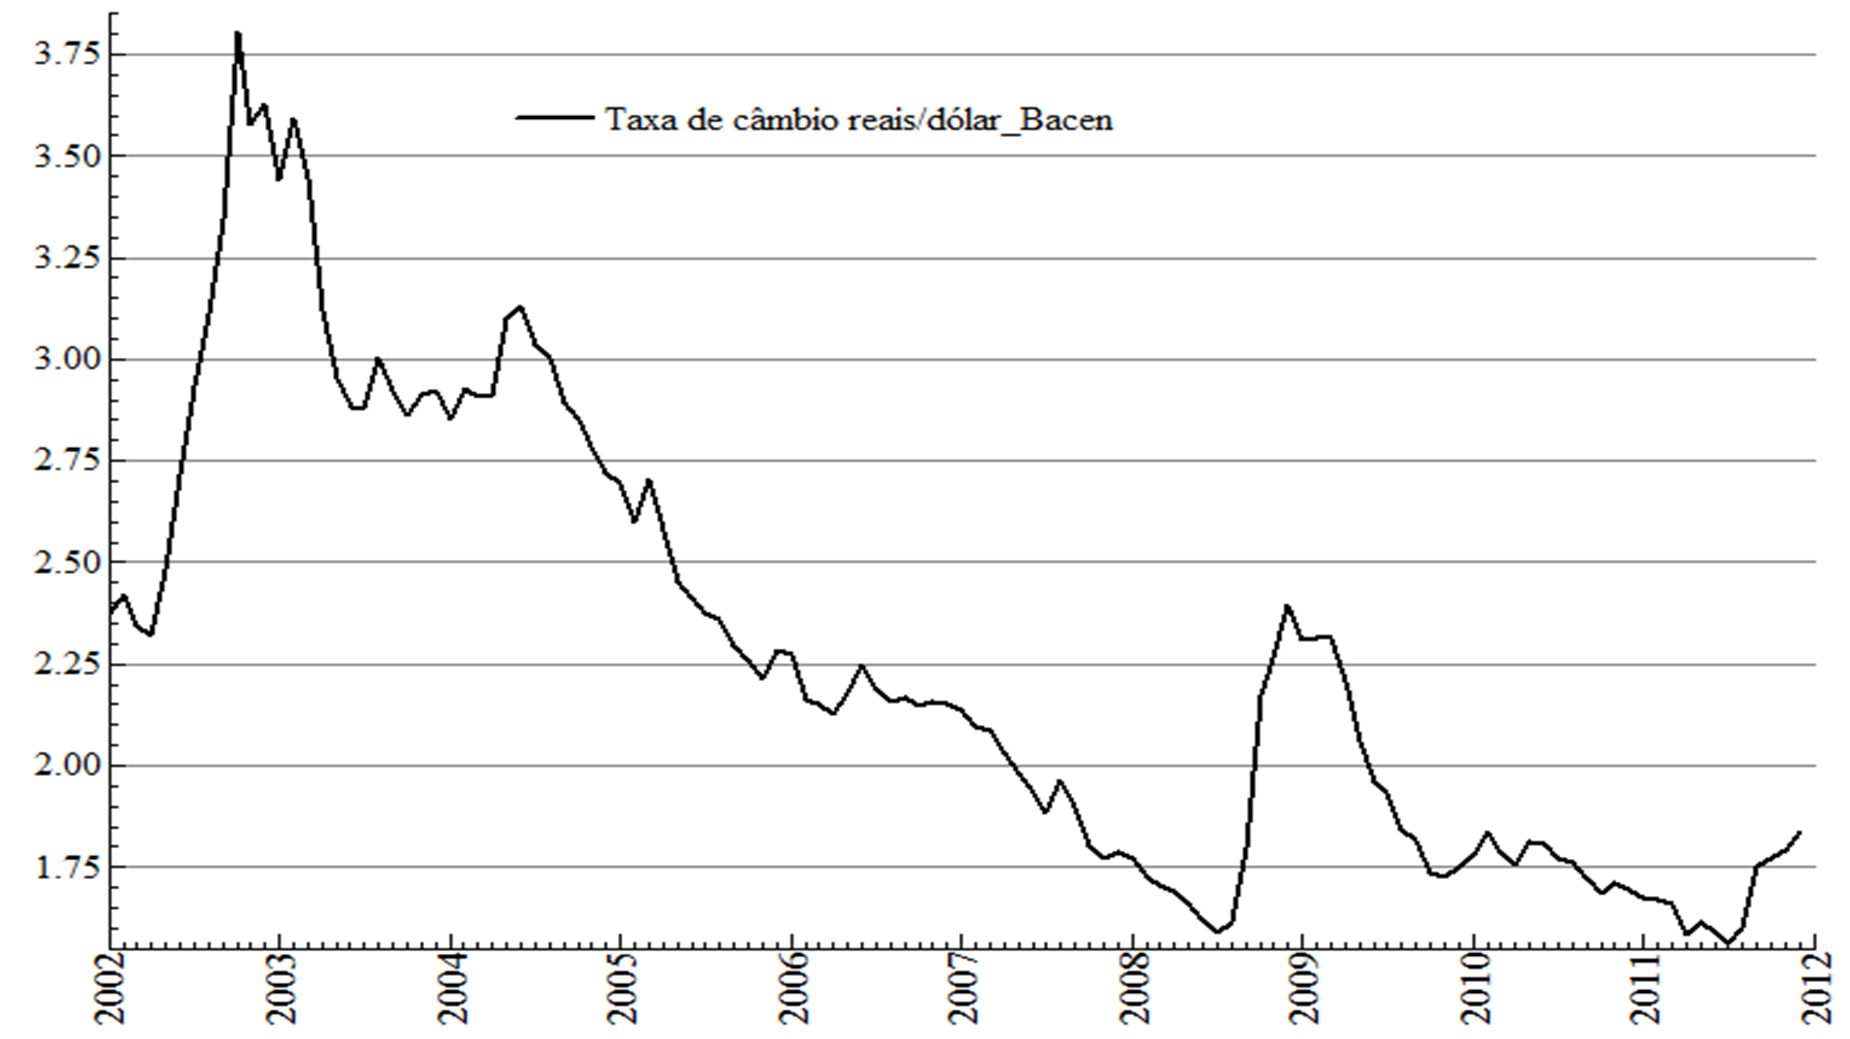
\includegraphics[width=0.7\linewidth]{Imagens/a16i2.png}
\end{figure}

A população via o governo da época (ainda FHC) se deteriorar, vendo a inflação subir, colocando toda a culpa sobre o governo, e não das ideias do partido opositor e como suas ideias estavam influenciando as expectativas do mercado, dado suas colocações em eleições(fracassadas) passadas.

\subsection{\textbf{O PT e a “Carta aos brasileiros”}}
O PT + Lula, não queria ser o governo que colocou o Brasil no buraco de novo, eles queriam vencer as eleições e ficar na política de maneira consistente. Lula então declara publicamente que José de Alencar(candidato de centro-direita do PL) para ser seu vice, mostrando ao mercado seu comprometimento com estabilidade e responsabilidade macro

Em 2002, Palocci (considerado moderado, um ponto fora da curva do PT) é nomeado coordenador do programa do governo(mais um agente para influenciar o mercado para passar confiança aos agentes):\begin{itemize}
    \item abriu diálogo com agentes do mercado(principalmente o financeiros), defendendo que o PT tinha mudado. Junto também do José de Alencar
\end{itemize}

Em junho de 2002, o PT lança(Palocci escreve e Lula publica):
\begin{itemize}
    \item a ``Carta aos brasileiros'', que defendia o superávit primário; comprometimento do partido, chapa e representantes com a política de boa gestão.
    \item um programa de governo mais moderado; ao contrário do que os agentes do mercado e seus discursos anteriores diziam; comprometido com o tripé macro(promessa e discurso não são governo, isso ajuda a diminuir o risco país, mas nem tanto)
    \item uma nota que promete respeitar acordo negociado com o FMI.
\end{itemize}

\textbf{Como entender/explicar essa mudança de pensamento?}

\subsection{\textbf{Qual era o cenário econômico com novo governo já eleito? (final de 2002)}}

Lula e coalizão sabia que eles sabiam que não podiam romper com processo de econômico de estabilização. 

O superávit de 3,75\% do PIB acordado com o FMI para 2003 parecia ser insuficiente:

\begin{itemize}
    \item Um aumento indicaria compromisso fiscal do novo governo;
    \item E a escalada do câmbio, provavelmente, traria aumento da inflação e exigiria elevação da taxa de juros;
    \item A relação dívida/PIB havia aumentado bastante.
\end{itemize}

A expectativa média do mercado para o IPCA tinha subido de 4\% para 11\% ao longo de 2002.

Fazer ajuste fiscal e elevar a taxa de juros era tudo que o PT não desejava fazer, considerando seu histórico de propostas.  
Assim, a economia brasileira vivia o auge da incerteza.

\subsection{\textbf{Primeiras medidas (final de 2002 e início de 2003)}}
Para garantir boas práticas ele indicou "bons" nomes(ministros; Palocci o indicado como Ministro da Fazenda do governo Lula e também responsável por ir atrás de bons nomes para sua equipe econômica(Henrique Meirelles para presidente do BC; José Scheinkman como autor da agenda perdida e indicou ao Palocci essa agenda, apesar do Scheinkman não fazer parte da equipe mas fez sua contribuição, além do Scheinkman do indicar o Marcos Lisboa(avesso ao PT) para ajudar Palocci entender a ideia da agenda perdida, assim o Lisboa secretário de política econômica, pois ele viu que o PT queria uma equipe competente) para fazer parte do seu governo, trazendo segurança para os agentes do mercado, o que ajudou a a reduzir o risco país.

Palocci, no início de 2003, é anunciado Ministro da Fazenda em conjunto com o documento: 
\textit{``Política econômica e reformas estruturais''}

\begin{itemize}
    \item A ideia seria manter a estabilidade econômica e redirecionar os gastos públicos às classes sociais mais necessitadas.
\end{itemize}

Nomeado Henrique Meirelles presidente do Bacen (mantida toda diretoria anterior)

Metas de inflação de: 8,5\% e 5,5\% para 2003 e 2004 (bem menores que a de 2002)

Elevou a taxa de juros Selic

\subsubsection{\textbf{Primeiras medidas e superação da crise de 2002}}
Definiu superávit primário em 4,25\% do PIB em 2003 (mesmo sem ser exigido pelo FMI)

Ordenou cortes de gastos e deixou na Lei de Diretrizes Orçamentárias a mesma meta fiscal para 2004-2006

Em suma: era o abandono de várias bandeiras históricas defendidas pelo PT

Era a conclusão de que austeridade e estabilidade deveriam ser políticas de Estado e não de partidos

Já no 2º trim., a taxa de câmbio era menor que R\$ 3,00 e o risco país inferior a 800 pontos

\begin{figure}[H]
    \centering
    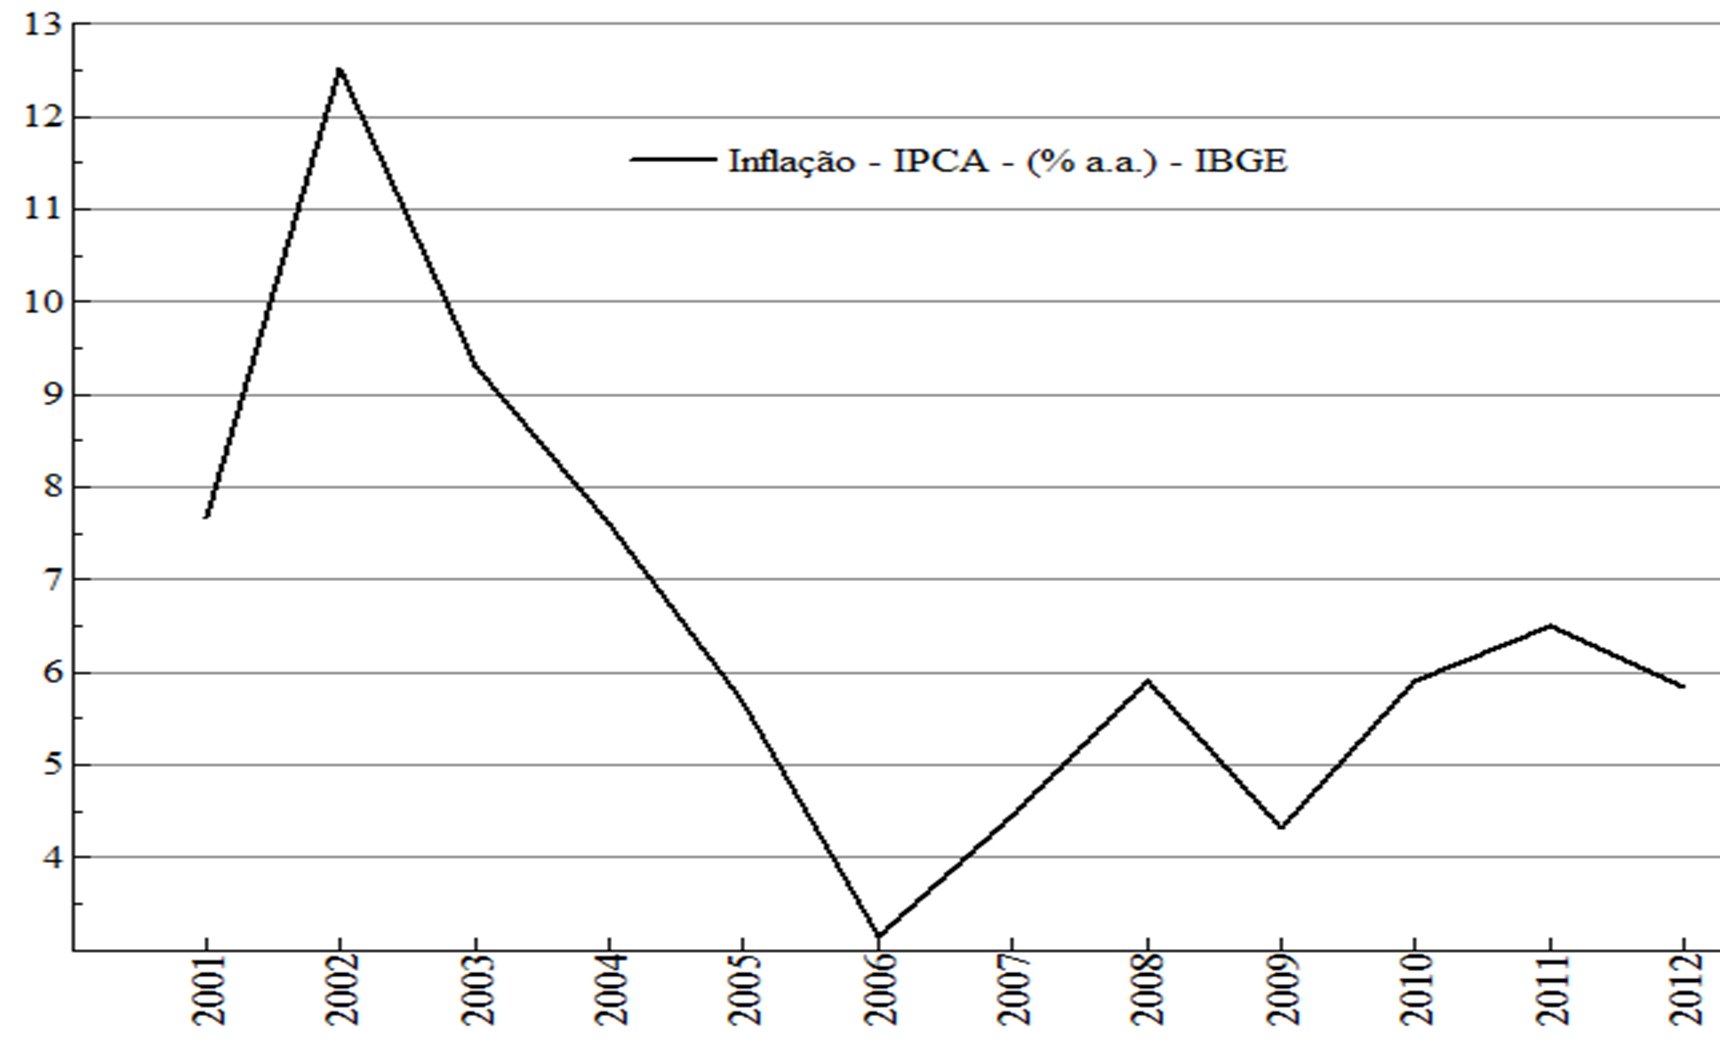
\includegraphics[width=0.7\linewidth]{Imagens/a16i3.png}
\end{figure}

\begin{figure}[H]
    \centering
    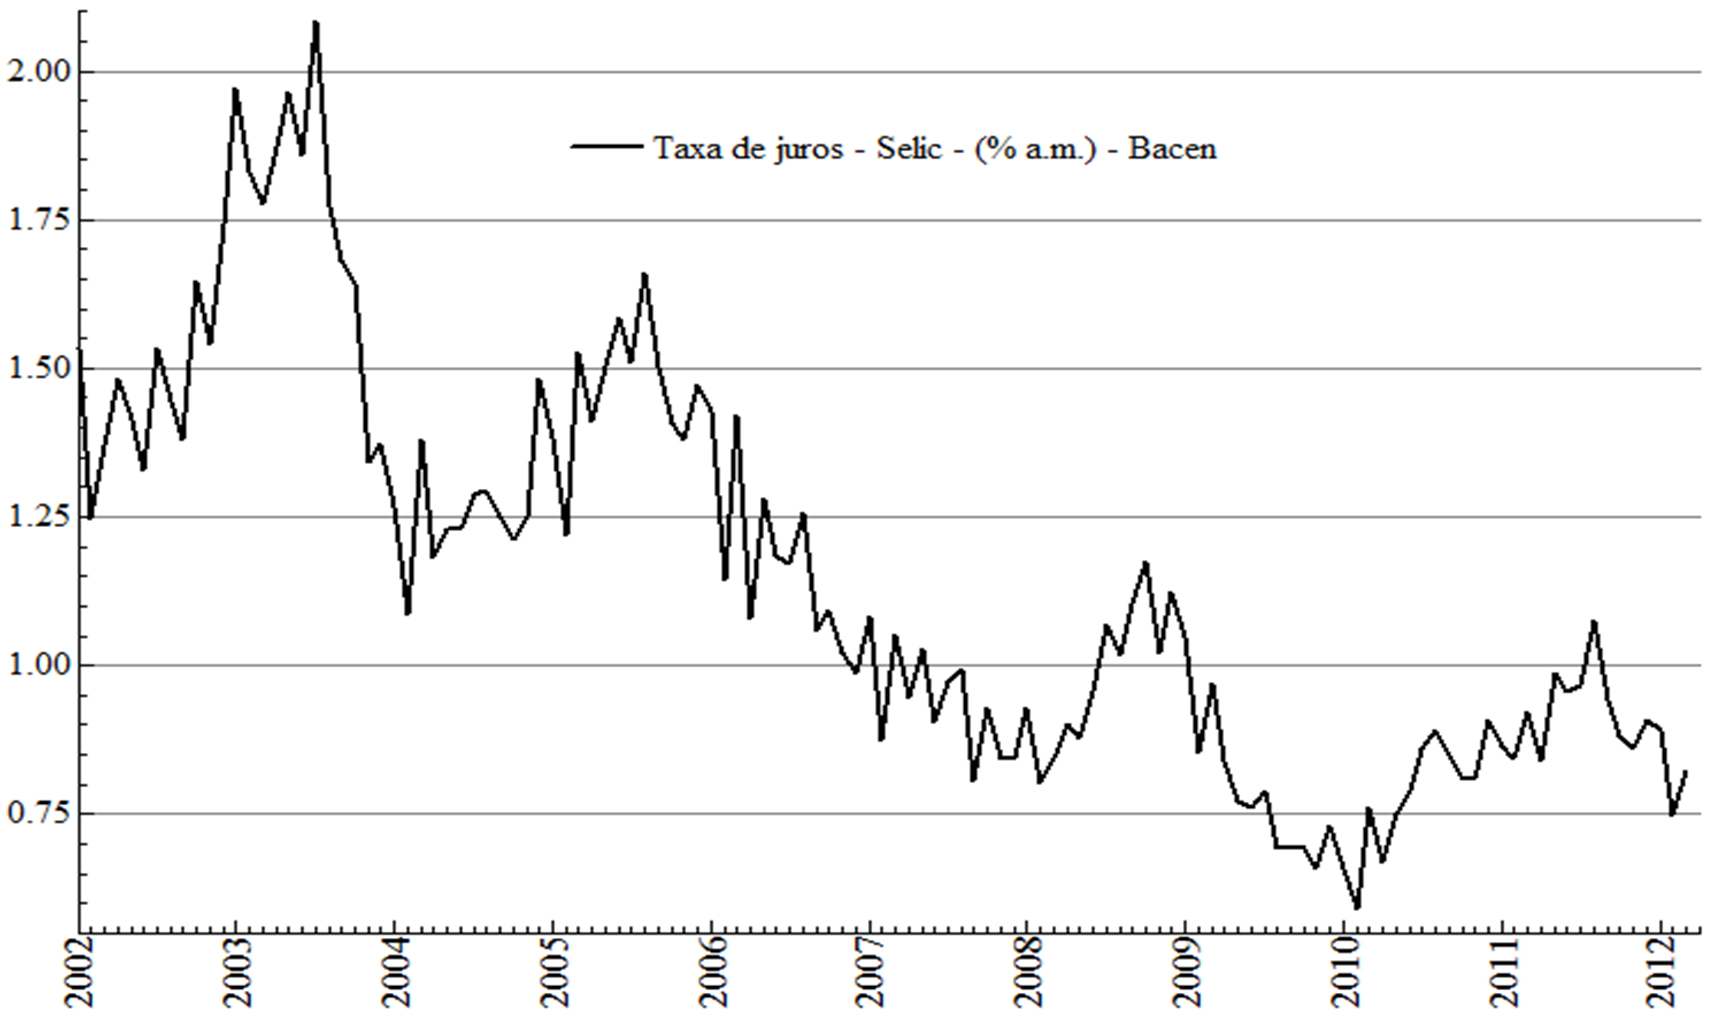
\includegraphics[width=0.7\linewidth]{Imagens/a16i4.png}
\end{figure}

\begin{figure}[H]
    \centering
    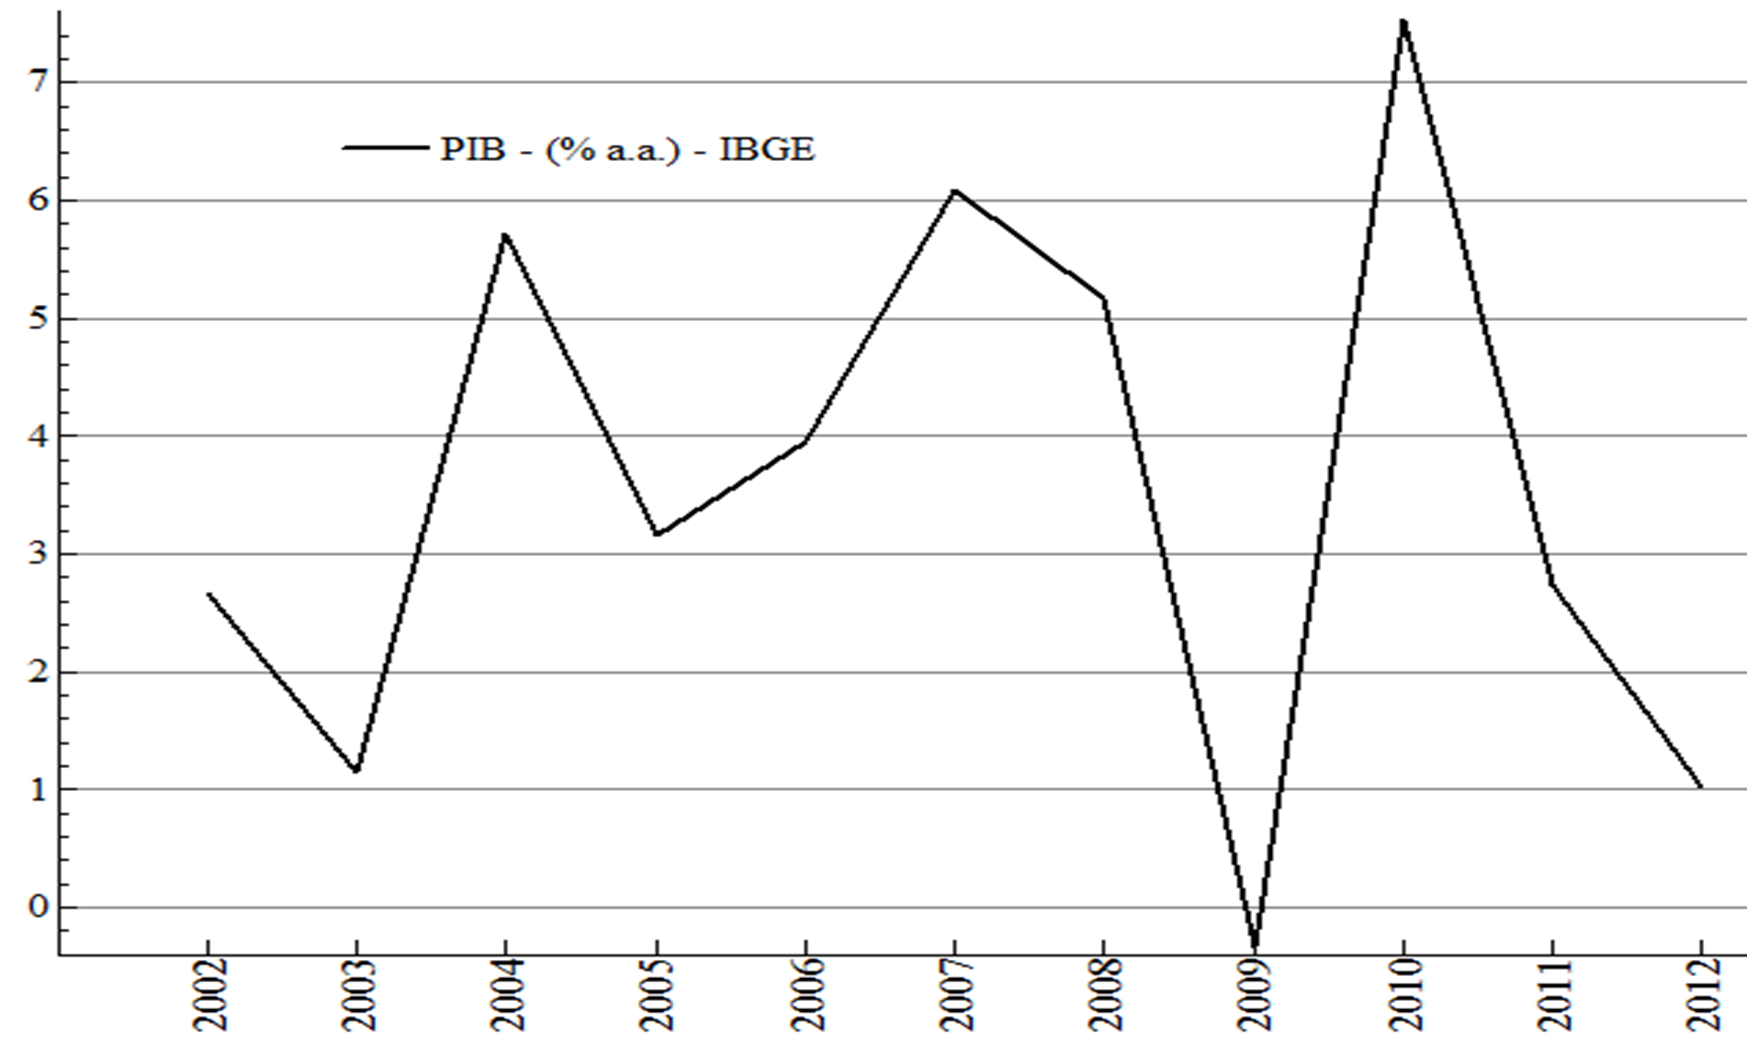
\includegraphics[width=0.7\linewidth]{Imagens/a16i5.png}
\end{figure}

\subsubsection{\textbf{Superação da crise de 2002}}
Esse movimento de organização de uma boa equipe e práticas responsáveis para reforçar o Tripé Macro, resultado disso foi uma maior confiança dos agentes econômicos(mercado), gerando uma queda abrupta do risco país. Gerando a superação da Crise de 2002

Ocorre a renovação do acordo com o FMI até final de 2004:

\begin{itemize}
    \item Mantido compromisso das metas fiscais;
    \item Brasil não precisou dos recursos (foi um acordo ``prevenção'');
    \item Sinal de que a prática de política econômica seria mantida.
\end{itemize}

Inflação demorou para recuar, pois a desvalorização havia sido alta.

\begin{itemize}
    \item Redução da Selic é promovida no segundo semestre de 2003.
\end{itemize}

Os ótimos resultados da balança comercial, respondendo ao câmbio e à melhor demanda externa, reforçaram a superação.

A sequência da política econômica teria o objetivo de buscar crescimento econômico e melhorar o setor externo.

\begin{figure}[H]
    \centering
    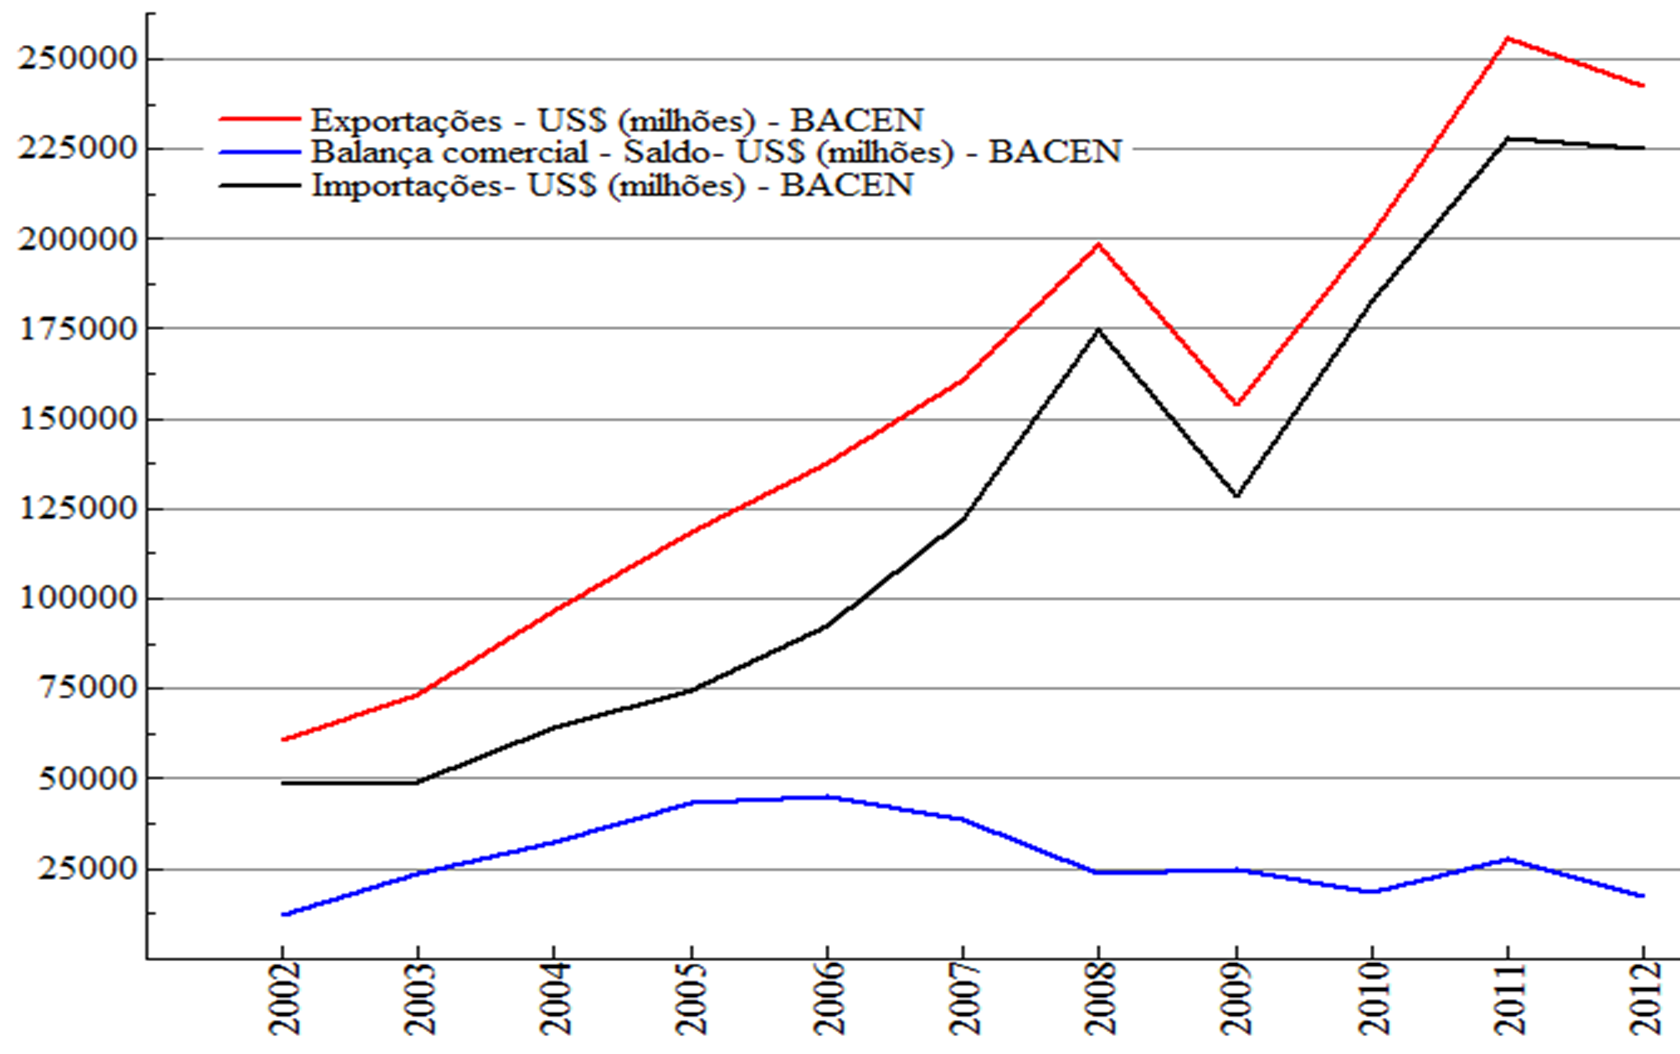
\includegraphics[width=0.7\linewidth]{Imagens/a16i6.png}
\end{figure}

A BP mais que dobra nesse período, saindo de quase 20 bi de dólares para quase 50 bi de dólares. Ocasionando em uma grande melhora da conta corrente nacional.

\begin{figure}[H]
    \centering
    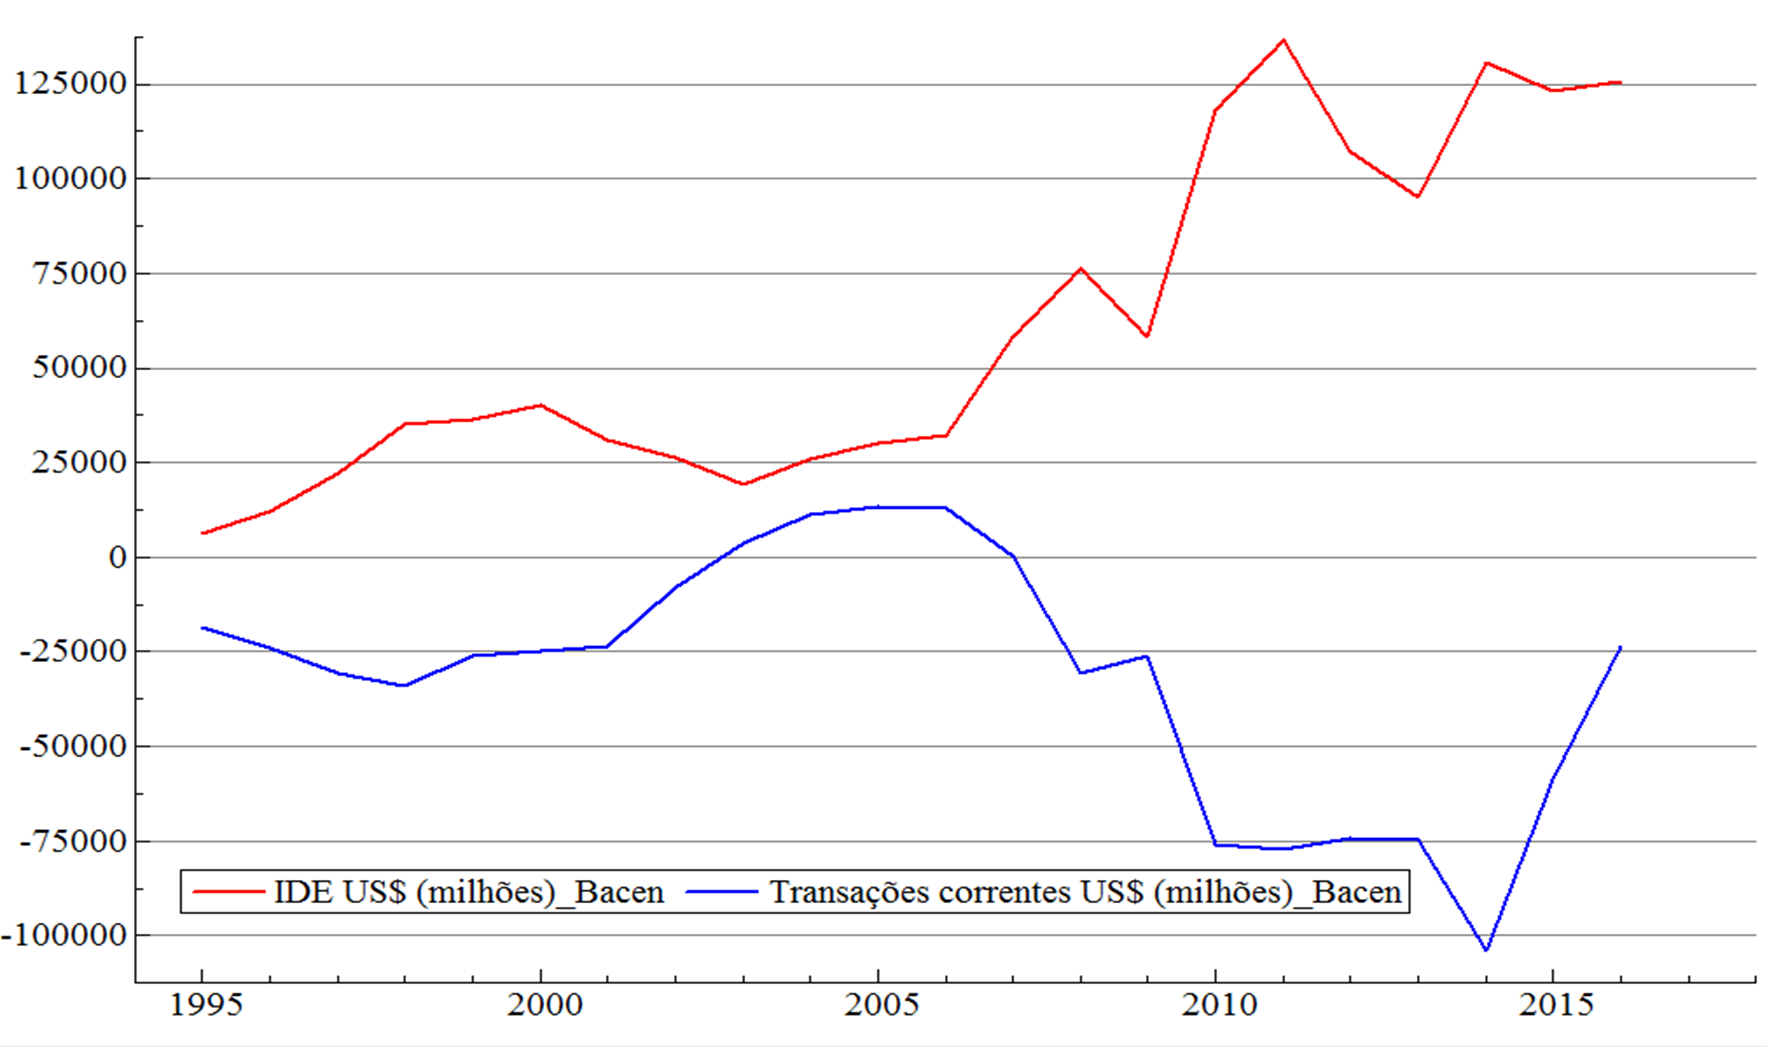
\includegraphics[width=0.7\linewidth]{Imagens/a16i7.png}
\end{figure}

\subsubsection{\textbf{O ano de 2003}}
A ortodoxia(com o seu tripé macro) trouxe queda das taxas de inflação (9,3\% em 2003). Além disso as reformas institucionais(enviadas ao congresso nacional) foi algo importantíssimo para os bons resultados econômicos desse governo.

Havia forte liquidez internacional (taxa americana de juros perto de 1\%)

Com a queda da taxa de inflação, a taxa real de juros subiu (6\% em 2002 para 13\% em 2003)
\begin{itemize}
    \item compromete desempenho do PIB.
\end{itemize}

Propostas de reformas(institucionais) são encaminhadas ao Congresso(iniciadas nos anos 2003 e aprovadas ao longo dos anos seguintes):
\begin{itemize}
    \item Tributária (manter CPMF, transforma Cofins sobre valor agregado)
    \item Mercado de crédito (\textit{ex}: crédito consignado), uma reforma micro. Exemplo :lei das falências, lei do crédito consignado(tomada do empréstimo e as parcelas desse empréstimos já seriam descontadas do salário de quem tomava o empréstimo, a expectativa de calote(risco calote) caí, já que está atrelado ao salário, isso reduz o juros do empréstimo, além de aumentar a quantidade de bancos que querem oferecer esse tipo de empréstimo. Uma mudança Institucional(sem existir subsídio), pode auxiliar no crescimento econômico.), lei do leasing. Isso está de acordo com a agenda ortodoxa.
    \item Previdência (concentra-se no regime de servidores públicos)
    \item reforçam as práticas de ajuste fiscal e de redução da desigualdade(melhoria social). O Estado oferece serviços públicos que são concentradores de renda, servidores tendiam a se beneficiar mais das políticas beneficiárias, e essas reformas acabariam com isso, isso gerou desavenças com a base eleitoral do governo do Lula/PT(os servidores públicos no caso). Reduzindo os gastos públicos com esse tipo de coisa.
\end{itemize}

O governo Lula 1 , entregou um crescimento econômico maior e melhor que o ocorreu no governo FHC. 

\subsection{\textbf{Política fiscal no período Lula 1}}
Foi mais contracionista que a do período FHC:

\begin{itemize}
    \item reduziu forte o gasto primário até 2004 e, a partir disso, voltou a aumentar, sendo financiado pela elevação da carga tributária;
    \item A política monetária trouxe deterioração das contas ao elevar os compromissos com juros.
\end{itemize}

\textbf{Síntese}
\begin{itemize}
    \item A apreciação cambial, em conjunto com a elevação do resultado primário, gerou um processo de queda consistente da relação dívida/PIB;
    \begin{itemize}
        \item Efeitos patrimoniais (dominados pela apreciação) foram responsáveis por quase 2/3 dessa queda (tab. 8.2, Giambiagi)
    \end{itemize}
\end{itemize}

\subsection{\textbf{Tendência cambial no governo Lula 1}}
A taxa real de câmbio brasileira apreciou significativamente:

\begin{itemize}
    \item Ambiente externo favorável: melhora dos termos de troca; boom de preços de commodities; forte liquidez internacional e juros baixos;
    \item Selic em tendência de baixa no geral, mas ainda elevada;
    \item Melhoria fiscal e do endividamento deixou as expectativas bastante favoráveis, reduzindo o risco país.
\end{itemize}

Boa parte das condições que geraram a apreciação cambial permitiram um rápido ajuste do setor externo:

\begin{itemize}
    \item O déficit em conta corrente de 1,7\% do PIB em 2002;
    \item Mudou para um superávit de 2\% do PIB em 2004.
\end{itemize}

\subsection{\textbf{O PT volta a ser PT? Melhor: a nova coalização pede mais intervencionismo?}}

Em 2005, a crise cambial tinha sido resolvida e o Brasil mostrava forte crescimento econômico, mas ``surge'' a Crise do Mensalão(Brasil é Brasil e Mundo é Mundo, nada de bom dura para sempre): \begin{itemize}
    \item Abala o núcleo político do PT (José Dirceu o ministro da casa civil, o mão direita do governo ) e a prática econômica inicial fica abalada;
    \item José Dirceu tinha sido central para a disciplina partidária no PT, evitando que os críticos à política econômica elevassem o tom; Havia um pagamento de mensalidade (por isso mensalão), para os senadores/pessoal do congresso votar de acordo com as políticas do Lula/PT
    \item O esforço de Lula agora era conter a crise política e garantir a reeleição;
\end{itemize}
José Dirceu, então ministro da Casa Civil, renuncia; Além disso Dirceu aceitava as propostas do Palocci, por mais que ele não concordasse, mas, por ele, assim que as coisas dessem certo, ele trocaria por medidas expansionistas. Ele era quem segurava guerra de quem queria derrubar isso, pois ele era fiel ao Lula, e como o Lula estava com Palocci, logo Dirceu estava com Palocci. Com sua saída, se criou um vácuo de "poder".

Dilma Rousseff, de Minas e Energia, assume a Casa Civil e ganha mais espaço no governo; Isso faz com que a política econômica e o Palocci se tornasse grandes alvas de críticas.

Palocci propõe uma medida de controle do crescimento dos gastos, mas sofre forte oposição dentro do PT (Dilma é o ``símbolo'')\begin{itemize}
    \item A medida não foi aprovada e(porque será ??), ainda, deixou mais fortalecidos os críticos de Palocci dentro do PT; Dilma era a mais contra a isso, surgindo o "Gasto é Vida"
    \item Palocci é acusado de abuso de poder, além de ter sido acusado de problemas quando era prefeito de Ribeirão Preto, ele renuncia e sendo substituído por Guido Mantega em março de 2006. Esse era contrário as medidas de Palocci, uma mudança total na equipe do Lula e do governo, e grandes mudanças na política fiscal vai ocorrer. Lembrando que o Lula estava com muitos pedido de impeachment.
\end{itemize}

Tentando mostrar diferença em relação à FHC (e ao ``Lula 1''), o governo lança o PAC(Programa de Aceleração de Crescimento) sob a liderança de Dilma em 2007 e Mantega:\begin{itemize}
    \item Era o abandono da ideia levantada em 2005 para incentivar investimentos privados em infraestrutura via melhoria dos aspectos de regulação (contexto de responsabilidade fiscal);
    \item Na visão de Dilma, era o momento de romper a tradição de contenção fiscal; estava na hora do estado ser mais intervencionista para ter auxílio fiscal a certos setores(privado em especial). Política Fiscal seria intervencionista (agenda heterodoxa nesse ponto)
    \item Denota a perda de espaço da Fazenda dentro do governo.
\end{itemize}

\textbf{O que explica essa nova reviravolta?}

\subsection{\textbf{Mudança da política fiscal}}
Há mudança significativa a partir da entrada de Mantega (2006):

\begin{itemize}
    \item Variação real do gasto aumenta (ex: aumentos do funcionalismo);
    \item Afrouxamento dos superávits primários. Ex: passou a gastar parte do superávit primário, descontando algumas despesas como os investimentos; Apesar dos resultados positivos e dentro das metas estabelecidas
    \item Abandonada a ideia de um plano de longo prazo para conter despesas;
    \item Governo não consegue renovar no Congresso a CPMF(Contribuição Provisória sobre Movimentação Financeira); a "intensão" do CPMF era para ajudar na saúde pública.
    \item Forte aumento do salário mínimo (acima da inflação) penalizou inúmeras despesas do governo;
    \item Eleva-se a importância do BNDES na economia (com recursos financiados pelo Tesouro, escolheu e ajudou grandes empresas).
\end{itemize}
w
Assim, houve forte expansão do crédito estatal, financiada pela emissão de dívida pelo Tesouro:

\begin{itemize}
    \item Compromisso era cada vez menor com as metas fiscais e maior era o uso de manobras contábeis;
    \item Lei de Responsabilidade Fiscal foi sendo desconstruída (ex: relação entre Tesouro e BNDES);
    \item Tesouro passou a transferir bilhões de reais ao BNDES sem que houvesse impacto no resultado primário e na dívida líquida;
\end{itemize}

Eram empréstimos de 30 anos com juros fortemente subsidiados;

Tesouro emite dívida, cresce a dívida bruta, mas não a líquida, porque o Tesouro ``se permitiu'' abater da dívida bruta, como ativos, os empréstimos ao BNDES;

Esse abatimento era ``criativo'';

Depois, parte desses empréstimos voltavam ao Tesouro, gerando:
    \begin{itemize}
        \item melhoria do superávit primário;
        \item compras do BNDES em favor do Tesouro a dividendos futuros da Eletrobrás e ações na Petrobras (ampliava participação do governo nas empresas);
    \end{itemize}

\textbf{Ou seja, a gestão fiscal parecia não ter mais restrição!}

\textbf{Empréstimos do Tesouro ao BNDES em 2008-14 }

\begin{figure}[H]
    \centering
    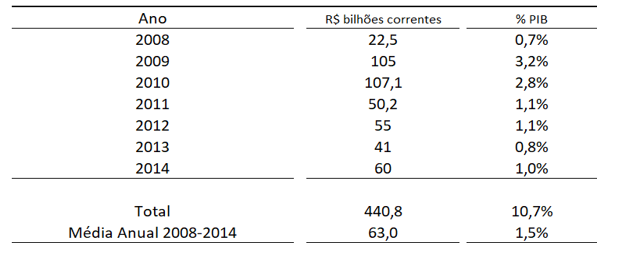
\includegraphics[width=0.7\linewidth]{Imagens/a17i1.png}
\end{figure}

\subsection{\textbf{Setor Externo}}
Acúmulo de reservas e apreciação cambial\begin{itemize}
    \item Há forte acumulação de reservas (RI) nos primeiros anos do Governo;
    \item Houve superávits nas contas correntes no início;
    \item Fluxo crescente de IDE;
    \item Consequentemente, redução da dívida externa líquida (Brasil se torna credor líquido a partir de 2008);
    \item É uma forte mudança, considerando o padrão histórico brasileiro.
\end{itemize}

Mas, como já vimos, houve apreciação cambial (revertida pós-2008):\begin{itemize}
    \item Assim, a conta de capitais explica o acúmulo de RI e não os resultados da conta corrente;
    \item A apreciação, em conjunto com a demanda interna aquecida, pressionaram as importações.
\end{itemize}

Por isso, os fluxos de capitais, a demanda externa e a alta das commodities:\begin{itemize}
    \item ``Protegeram'' o setor externo brasileiro da apreciação cambial.
\end{itemize}

\begin{figure}[H]
    \centering
    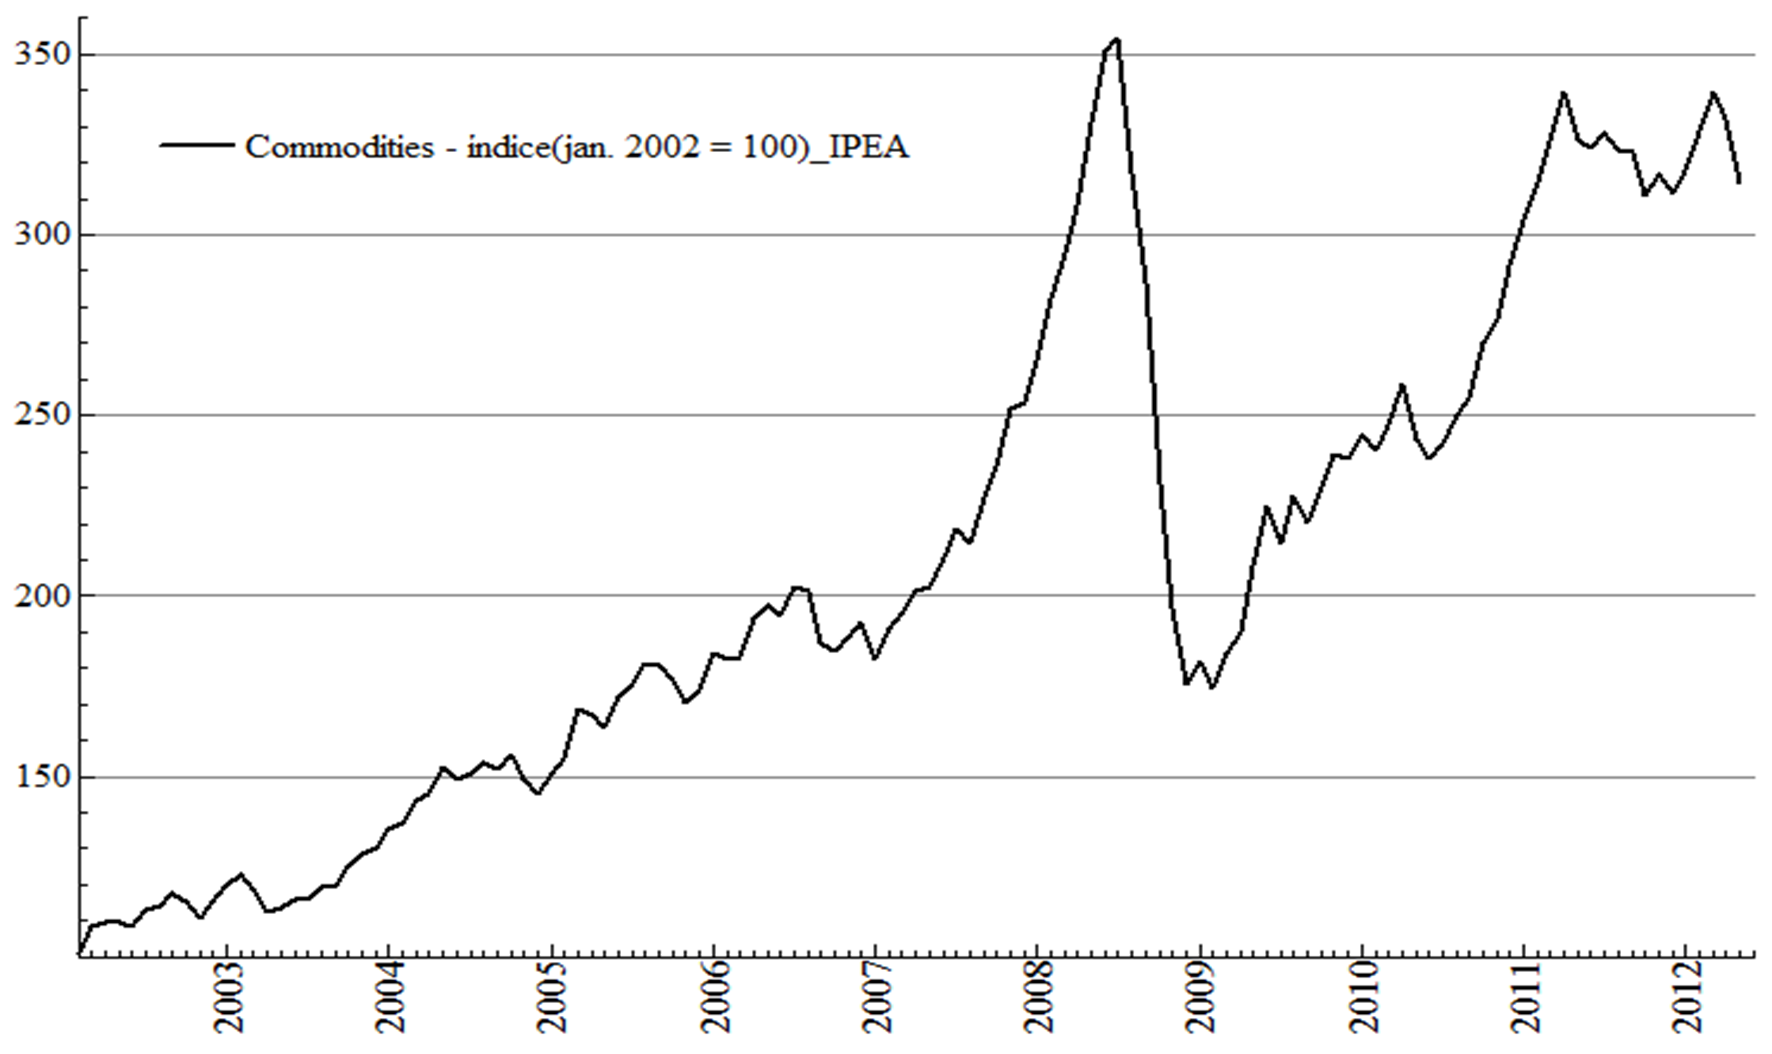
\includegraphics[width=0.7\linewidth]{Imagens/a16i8.png}
\end{figure}

\subsection{\textbf{Um novo contexto econômico}}
O 2º Governo FHC e primeiros anos de Lula mostraram:
\begin{itemize}
    \item Dificuldade do setor externo com pressões sobre o câmbio;
    \item Assim, a inflação esteve pressionada, o que exigiu juros crescentes, retirando a capacidade de crescer.
\end{itemize}

Agora a economia brasileira:
\begin{itemize}
    \item Apresentava taxas significativas de crescimento econômico;
    \item O setor externo estava protegido;
    \item Foi dado ao Brasil o ``selo'' de bom pagador pelas S\&P e Fitch em 2008 e em 2009 pela Moody’s;
    \item A taxa de inflação estava caindo e, portanto, as taxas de juros poderiam cair também, reforçando um ciclo virtuoso.
\end{itemize}

\textbf{Mas, a poupança doméstica caiu (consumo privado e do governo sobem)}

\subsection{\textbf{Nova realidade brasileira (formada ao longo dos anos 90 e 2000)}}
Tinha consolidado a estabilização;

Estabelecido uma relação mais aberta com exterior;

Setor externo e a dívida externa bruta pareciam equacionadas;

Conquistado forte prestígio no cenário internacional;

A importância crescente da economia chinesa (e Índia) no mundo (forte impacto sobre o Brasil, já que eram grandes importadores);

Descobertas do pré-sal (``seria a última grande descoberta do mundo'');

Produtor de etanol (petróleo atingia US\$ 100 e há preocupação crescente com o meio ambiente).

\subsection{\textbf{Diante desse novo contexto: A crise de 2008}}
Os anos anteriores indicavam elevação do crédito bancário e ampliação das inovações financeiras:
\begin{itemize}
    \item Estimulou o mercado imobiliário, gerando uma alta expressiva dos preços que terminou com um ``estouro da bolha'';
    \item Mercado de seguros foi contaminado e consequentemente o mercado financeiro;
    \item O banco de investimentos Lehman Brothers quebra (set. de 2008);
    \item Ocorre forte movimento de venda de ativos e reposicionamento dos agentes em cenário de grande incerteza.
\end{itemize}

Efeitos observados pela economia brasileira?
\begin{itemize}
    \item Reduz entrada de capitais;
    \item Reduz preços das commodities.
\end{itemize}

\subsection{\textbf{Nova realidade brasileira e a Crise internacional}}
Recuperação pós-crise de 2009:
\begin{itemize}
    \item Possuía reservas internacionais na ordem de US\$ 200 bilhões;
    \item Houve medidas de estímulos fiscais importantes;
    \item O sistema financeiro era sólido;
    \item Ou seja, boa parte das regras e instituições transformadas desde o início dos anos 90 reduziram a incerteza 
    (PROER tinha sido importante, Real, a consolidação do regime de metas que era acompanhado de melhoria fiscal e de câmbio flutuante).
\end{itemize}

Assim, o Brasil exercia atração para grande parte de investidores;

Por outro lado, foi o ``pretexto'' para reforço do ``modelo econômico'' iniciado desde 2006;
\begin{itemize}
    \item Governo ficou mais ``à vontade'' para defender maior intervenção na economia.
\end{itemize}

\begin{figure}[H]
    \centering
    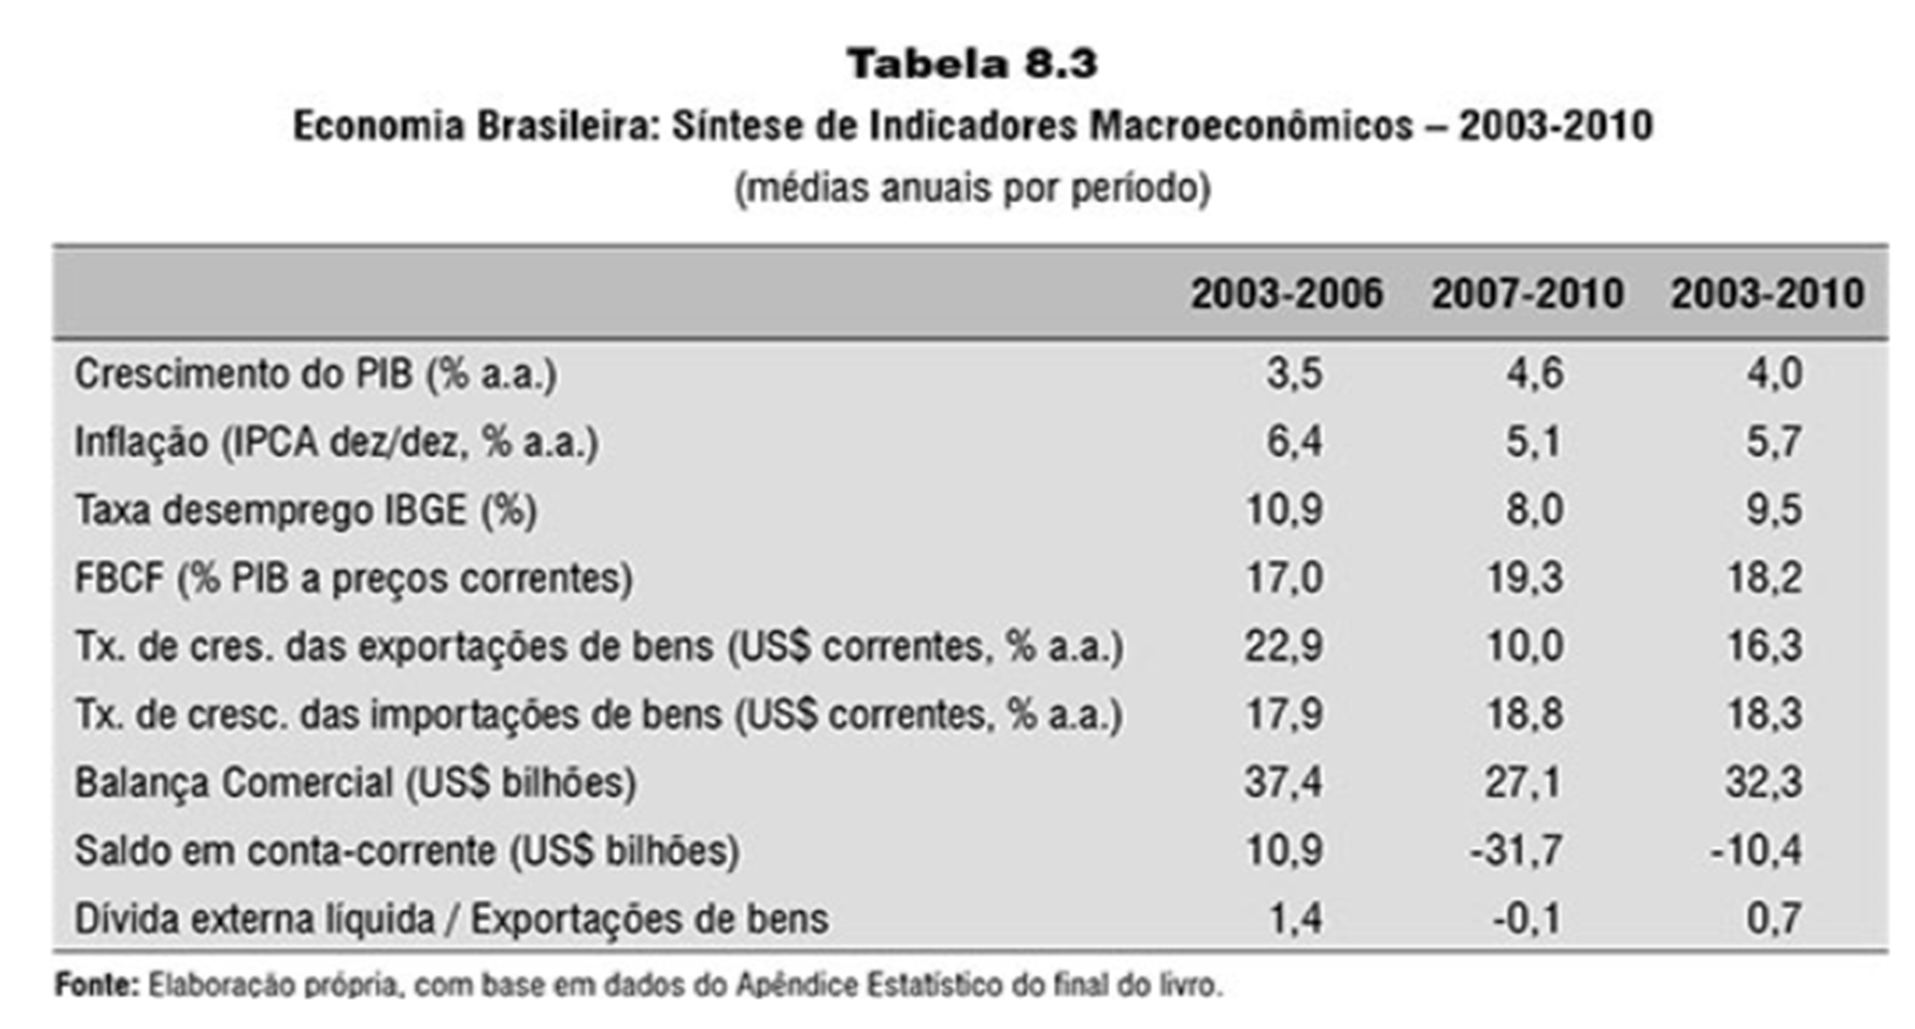
\includegraphics[width=0.7\linewidth]{Imagens/a16i9.png}
\end{figure}

\subsection{\textbf{Atividade econômica e preços}}
No geral, os resultados foram positivos:
\begin{itemize}
    \item Recuperação da crise de 2008 foi rápida;
    \item Inflação foi declinante;
    \item A taxa de desemprego também mostrou queda (de 12\% em 2002 para 7\% em 2010);
    \item A taxa de formalização da economia aumentou ($\uparrow$ arrecadação).
\end{itemize}

\subsection{\textbf{Cenário fiscal a partir de 2009}}

Deriva da crise internacional de 2008:
\begin{itemize}
    \item Economia brasileira para de crescer;
    \item Há perdas de arrecadação;
    \item Governo fornece incentivos, adotando uma política anticíclica;
    \item Crescimento anual do gasto primário foi de 6\% em termos reais (2005--2010), havia sido 2\% nos dois primeiros anos;
    \item Aumentam: transferências diretas (aposentadorias, salário mínimo com aumentos reais, seguro desemprego e Bolsa Família).
\end{itemize}

\textit{\textbf{Resultado:}} há redução do superávit primário e aumento da dívida pública.

Mas, neste contexto, o Brasil é credor líquido do exterior:
\begin{itemize}
    \item Reservas internacionais (RI) superam à dívida externa bruta;
    \item Agora, uma variação cambial apresenta efeito oposto: efeito fiscal de uma crise externa é positivo;
    \item A desvalorização de 2008 reduziu a dívida pública;
    \item E a apreciação em 2009 a fez aumentar (pois, o valor em R\$ das reservas tinha reduzido).
\end{itemize}

\textbf{Obs.:} RI = ativo que descontado da dívida externa bruta, traz o conceito da dívida externa líquida (DEL = DEB – RI).

\begin{figure}[H]
    \centering
    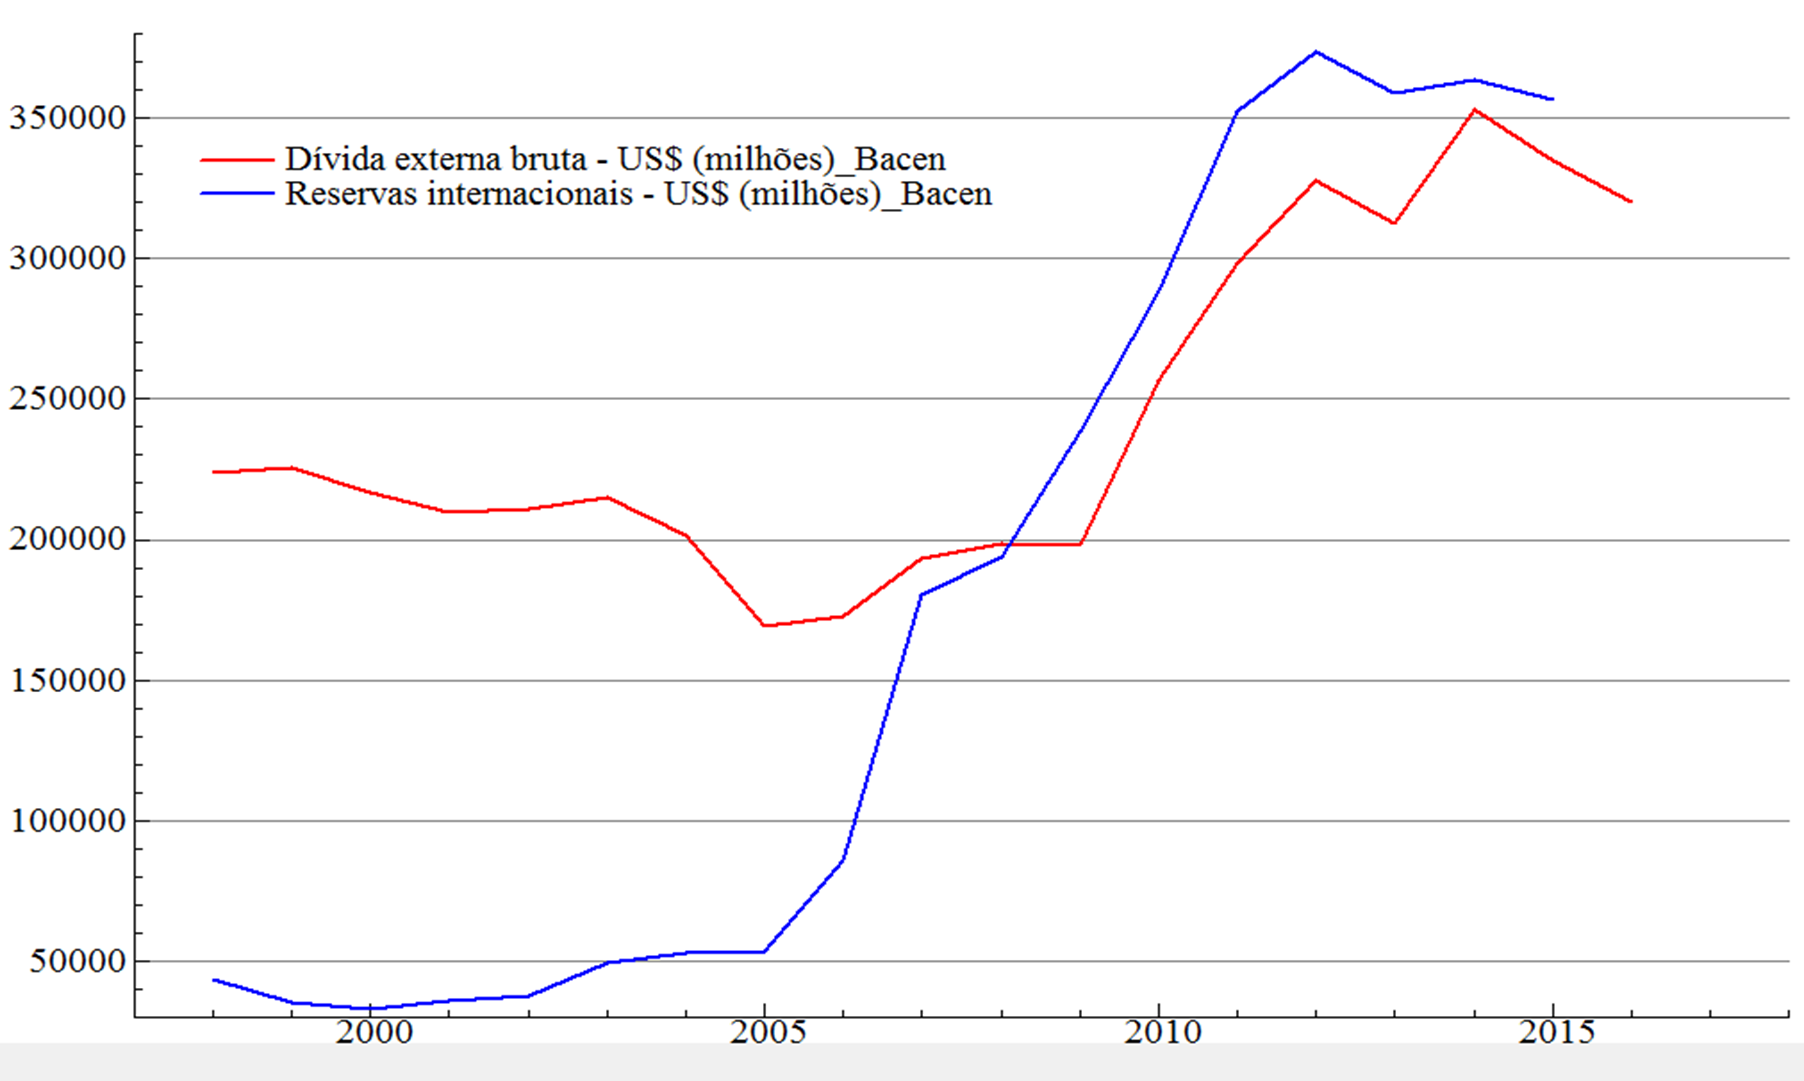
\includegraphics[width=0.7\linewidth]{Imagens/a16i10.png}
\end{figure}

\subsection{\textbf{Políticas redistributivas}}
Foi um dos marcos das campanhas eleitorais do PT ousar na redistribuição de renda;

Implementou o Bolsa Família:
    \begin{itemize}
        \item Unificou programas anteriores de transferência de renda, tornando-os mais abrangentes;
        \item Os benefícios exigiam cumprir itens quanto à nutrição, à saúde e à frequência escolar das crianças;
        \item Focalizou nas camadas de renda mais baixas e seu custo era relativamente baixo (0,4\% do PIB);
        \item Número de famílias atendidas passou de 3,6 milhões em 2003 para 11 milhões em 2006 e 12,8 em 2010.
\end{itemize}

Além disso, adotou uma política de reajuste do salário mínimo acima da inflação (salário cresceu 155\% e IPCA 56,7\%, 2003--2010).

\subsection{\textbf{Quais eram os desafios?}}
Combater a alta conjuntural de preços em 2010

Reduzir a meta de inflação para um nível mais próximo dos países avançados

Conciliar o regime de metas com um crescimento mais sustentado e forte

Conseguir um contexto de juros reais menores (considerando os desafios de meta mais baixa e de crescimento mais alto)

O que falta para a economia brasileira enfrentar esses desafios?\begin{itemize}
    \item Estrutura fiscal;
    \item É uma economia em desenvolvimento, assim choques externos trazem forte volatilidade cambial;
    \item Aspectos micro: produtividade (qualidade da educação, infraestrutura, ambiente de negócios, abertura comercial, estabilidade da política econômica) 
\end{itemize}

\newpage
\section{\textbf{Problemas econômicos e política econômica(O período Dilma Rousseff 2011-2016)}}

\subsection{\textbf{Temas e uma introdução}}

Herança econômica e desafios potenciais para o governo de Dilma Rousseff

Heterodoxia parece ter mais força dentro do governo

Escolhas tomadas, Nova Matriz Econômica (NME) e desdobramentos observados

\textbf{Leitura}: Economia Brasileira Contemporânea, (Cap. 9). Essa leitura pode ser substituída por – Coletânea “Sob a Luz do Sol – Uma Agenda Para o Brasil”, do Centro de debate de políticas públicas, particularmente o cap. 1. A política econômica do governo Dilma: a volta do experimentalismo \url{https://cdpp.org.br/wp-content/uploads/2017/02/CAPITULO-1.pdf}

\subsection{\textbf{Desafios}}
O governo Rousseff não tinha “espaço” para erros de política econômica, pois os desafios eram significativos

Existiam desafios estruturais, pois a expansão econômica observada no governo anterior tinha deixado a capacidade de oferta quase toda ocupada\begin{itemize}
    \item Houve expansão fiscal, principalmente, para enfrentar o cenário pós Crise de 2008;
    \item Taxa de desemprego estava baixa;
    \item Havia baixa ociosidade na capacidade industrial;
    \item Declínio do bônus demográfico nos anos 2010;
    \item População esperava continuidade do crescimento elevado;
    \item Custo mais elevado de formar a coalizão presidencial.
\end{itemize}

Ademais, havia uma pressão conjuntural de alta de preços (elevação das commodities e expansão fiscal)

Assim, era consenso (inclusive no governo) que o Brasil necessitava de uma onda de investimentos

Essa onda criaria capacidade oferta, permitindo manter o crescimento elevado sem gerar pressões inflacionárias

Mas como gerar uma onda de investimentos?

\begin{itemize}
    \item Ortodoxia (previsibilidade macro, ambiente regulatório, instituições, produtividade)
    \item Versus
    \item Heterodoxia (Governo toma ações que estimula consumo da população e beneficia setor privado e este realiza investimentos, dando “garantia” de lucro para seus investimentos)
    \item \textbf{Vitória} do discurso/lógica heterodoxa, junto da base de apoio eleitoral
\end{itemize}

\subsection{\textbf{Política econômica do governo (síntese)}}
No primeiro semestre de 2011, o governo esboçou uma agenda ortodoxa

\begin{itemize}
    \item Selic respondeu à elevação das expectativas inflacionárias;
    \item Política fiscal foi contracionista.
\end{itemize}

Mas a coalizão do governo Dilma Rousseff se estruturou com o passar do tempo, indicando ter grande apreço pela heterodoxia, bem acima da coalizão formada pós 2005

Assim, podemos justificar e entender a lógica das decisões de política econômica no governo Rousseff a partir do segundo semestre de 2011

Mas qual foi o significado prático dessas mudanças?

\begin{itemize}
    \item Total desestruturação do tripé macroeconômico;
    \item No lugar, implementada a nova matriz econômica (NME)
\end{itemize}

No geral, eram escolhas mais intervencionistas com ampliação dos gastos e muitos benefícios creditícios e tributários para o setor privado

\subsection{\textbf{Diagnóstico do Governo}}
Porque o setor privado não realiza investimentos?

Dois preços estavam “errados”, câmbio e juros

\begin{itemize}
    \item forçou depreciação (intervenções frequentes no mercado cambial);
    \item promoveu forte redução das taxas de juros (seria a marca do governo);
    \item consequentemente, perseguir a meta de inflação passou a ser um objetivo ambíguo (a meta seria alcançada, mas no próximo ano).
\end{itemize}

\subsection{\textbf{Nova matriz econômica (NME)}}
\textbf{Lógica}: incentivar crescimento econômico (acelerar investimentos)

\textbf{Raciocínio}: reduzir a carga fiscal (desonerações tributárias para diversos setores) + consumo de massas + redução dos juros + câmbio competitivo = onda de investimentos

\begin{itemize}
    \item mudanças frequentes nas regras para fluxos de capitais estrangeiros;
    \item intervenções frequentes no mercado de câmbio;
    \item juros subsidiados via agências públicas (BNDES), buscando reduzir os juros de mercado;
    \item mudanças no regime tributário (desonerações) aplicadas a diversos setores;
    \item controles de preços em certos setores;
\end{itemize}

\subsection{\textbf{Política monetária}}
“O divisor de águas” — a decisão do COPOM de agosto de 2011

Diante de expectativas de inflação acima do centro da meta, o Bacen reduz a taxa básica de juros! Qual era o raciocínio?

\begin{itemize}
    \item o cenário internacional traria um movimento contracionista (preços em baixa);
    \item a taxa de juros, então, tinha espaço para ser reduzida;
\end{itemize}

Consequências (incerteza quanto ao regime de metas):

\begin{itemize}
    \item na prática a taxa de juros teria deixado de ser o instrumento para se tornar o objetivo?
    \item o Bacen teria perdido a autonomia operacional?
\end{itemize}


\subsection{\textbf{Política fiscal}}
\begin{figure}[H]
    \centering
    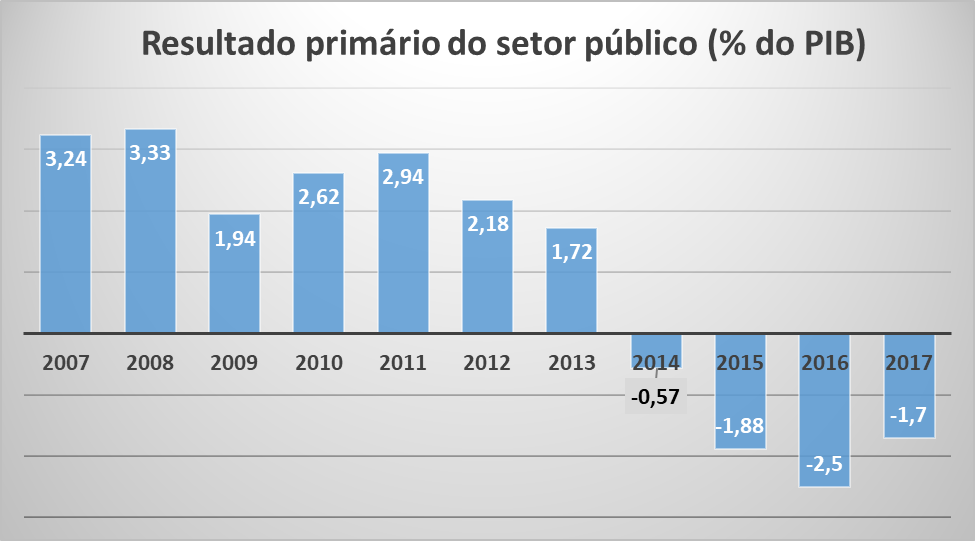
\includegraphics[width=0.7\linewidth]{Imagens/a18i1.png}
\end{figure}

O pós 2011 mostra, no geral, aprofundamento forte das práticas iniciadas no final do período Lula;

\begin{itemize}
    \item O governo “abriu mão” de arrecadação tributária (desonerou diversos setores), chamado de gasto tributário;
    \item Aos estados foi permitido endividamento junto aos bancos oficiais, na prática viabilizava gastos com pessoal (abandono da LRF!);
    \item No conjunto havia elevação de despesas e renúncia de receitas (sob a lógica de estimular investimentos);
    \item Houve aprofundamento das práticas da contabilidade criativa e ganharam a denominação de “pedaladas fiscais”;
\end{itemize}

\subsection{\textbf{Qual foi o resultado das novas lógicas monetária e fiscal?}}
As reversões dos regimes monetário e fiscal moldaram um cenário de forte incerteza econômica

\begin{itemize}
    \item A previsibilidade e estabilidade macro deterioraram, progressivamente, a partir de 2012;
    \item Isso causaria deterioração das expectativas.
\end{itemize}

Consequências ao longo do tempo:

\begin{itemize}
    \item queda da taxa de investimento e da PTF;
    \item As expansões monetária e fiscal geraram aumento do consumo no curto prazo;
    \item As expansões monetária e fiscal e intervenções cambiais trouxeram pressão inflacionária no médio prazo;
    \item O governo reagiu, aumentando intervenções e as desonerações;
    \item Mas a inflação cresceu e o Brasil entrou em recessão.
\end{itemize}

\subsection{\textbf{Algumas intervenções setoriais}}
Os setores elétrico e de combustível sofreram intervenções ao longo do tempo

\begin{itemize}
    \item No curto prazo os preços controlados aumentam a renda disponível das famílias e o consumo cresce; (a arrecadação aumenta e custos do setor privado declinam)
    \item Mas, no médio prazo as expectativas de inflação sobem já que em algum momento a inflação será recomposta; (reforça necessidade do Bacen elevar a Selic, impactando o fiscal e o desempenho econômico)
    \item Também, no médio prazo, a capacidade de investir desses setores declina já que a posição financeira deles deteriorou com o controle de preços; (o valor de mercado dessas empresas declina)
    \item O governo, no médio prazo, irá recompor os prejuízos financeiros desses setores, evitando a quebra desses setores e que a população perca a oferta desses serviços; (deteriora a posição fiscal)
    \item Síntese: uma intervenção deve ser muito bem avaliada, pois tende a gerar efeitos de curto e médio prazos e eles podem ser positivos ou negativos.
\end{itemize}

\subsubsection{\textbf{Outro caso de intervenção: FINAME}}
Ex: Dentro do PSI (Programa de Sustentação do Investimento) – financiamento para aquisição de máquinas e equipamentos (FINAME)

\begin{itemize}
    \item parte da capitalização do BNDES pelo Tesouro foi utilizada para linhas de crédito especiais;
    \item juros subsidiados (menor do que a inflação em alguns casos) para compra de caminhões para micro, pequenas, médias e grandes empresas;
    \item os tomadores de subsídio deveriam comprar de produtores locais (RCL);
    \item o preço do combustível estava controlado, desemprego era baixo, houve carência de 2 anos (2012/14);
    \item ao longo do tempo gerou excesso de oferta de caminhões, deixando o valor do frete menor;
    \item o cenário econômico deteriorou bastante ao longo dos anos;
    \item caminhoneiros estavam endividados, combustível com elevado preço (petróleo e depreciação), economia em recessão. Resultado?
    \item Greve dos caminhoneiros em maio de 2018!
\end{itemize}

\subsection{\textbf{Políticas sociais}}
Mesmo com o Bolsa Família, 22 milhões de pessoas continuavam na extrema pobreza

Plano Brasil sem Miséria (BSM) foi lançado em 2011

\begin{itemize}
    \item objetivo era superar a extrema pobreza até final de 2014;
    \item garantir a renda;
    \item fazer uma inclusão produtiva (Pronatec – oferece cursos gratuitos de qualificação profissional para público de baixa renda);
    \item dar acesso a serviços públicos (“Água para todos” – água para famílias do semiárido);
    \item foi dada atenção para uma evolução infantil saudável (mais vagas em creches e distribuição de vitaminas);
    \item o programa retirou 8 milhões de crianças e adolescentes da extrema pobreza (Brasil saiu do “Mapa Mundial da Fome”);
    \item avançou a custos baixos (0,5\% PIB no primeiro governo Dilma)
\end{itemize}

Conjunto de críticas:

\begin{itemize}
    \item restou a dúvida sobre a efetividade dos programas eliminarem carências importantes na saúde e na educação, que demandam políticas específicas;
    \item Foco? Pessoas em melhores condições financeiras tiveram acessos (FIES e “Ciência sem Fronteiras”), mas sem alcançar universalização efetiva aos direitos básicos.
\end{itemize}

\subsection{\textbf{A guinada de 2015}}
O final de 2014 indica que o cenário estava agravado e o ano seguinte estava sob forte incerteza

\begin{itemize}
    \item piora do déficit em conta corrente e das contas fiscais;
    \item a meta de inflação para 2015 estava desacreditada;
    \item forte crise política agravada com a Operação Lava Jato;
    \item setor elétrico estava deteriorado;
    \item elevação dos salários reais tinha reduzido as desigualdades, mas houve perda de competitividade do país;
    \item o investimento estava em queda há seis trimestres consecutivos;
    \item havia risco de perda do selo de bom pagador.
\end{itemize}

Ao ser reeleita, Dilma substitui Mantega por Joaquim Levy

\begin{itemize}
    \item algo politicamente complicado, pois Dilma estava sem apoio e agora perdia sua base eleitoral (“estelionato eleitoral”)
\end{itemize}

\subsection{\textbf{Medidas em 2015}}
O início do segundo mandato de Dilma é o oposto do primeiro.

Medidas do Ministro Levy:

\begin{itemize}
    \item programa de ajuste fiscal para recuperar o superávit primário;
    \item reduzir desonerações e tarifaço (aumento do preço da energia);
    \item forte redução dos investimentos (dentro da redução dos gastos).
\end{itemize}

O Bacen manteve a elevação da taxa de juros

\begin{itemize}
    \item a ideia era conter o efeito do reajuste das tarifas de energia;
    \item Agravou ainda mais a posição fiscal e a capacidade de crescer;
    \item a meta de 2015 seria rompida, mas haveria espaço para redução em 2016.
\end{itemize}

\subsubsection{\textbf{Medidas de 2015 e o fim do governo}}
Governo transfere para o Congresso a saída da crise e propõe:

\begin{itemize}
    \item reestabelecer a cobrança da CPMF, mas não consegue;
    \item péssima repercussão frente aos mercados;
    \item era um sinal de não governabilidade;
    \item em setembro de 2015 a S\&P divulga que o Brasil havia perdido o selo de bom pagador.
\end{itemize}

As crises econômica e política são fortes e Dilma substitui Levy por Nelson Barbosa

\begin{itemize}
    \item a ideia era tentar acalmar a base política;
    \item mas a crise se agrava em 2016 e em agosto a presidente Dilma perde seu mandato.
\end{itemize}

\subsection{\textbf{O primeiro ano da nova matriz econômica : Artigo de Guido Mantega}}
O primeiro ano da Nova Matriz Econômica (NME), implantada pelo governo Dilma Rousseff a partir de 2011, representou uma inflexão relevante nas diretrizes de política econômica do país. Essa estratégia visava um salto de competitividade aliado à continuidade da inclusão social e à redução das desigualdades, pilares herdados da década anterior.

A justificativa central da NME estava na correção de duas distorções estruturais da economia brasileira: \textit{juros elevados} e \textit{câmbio valorizado}. O governo argumentava que esses fatores desestimulavam o investimento produtivo e encareciam o financiamento da dívida pública, desviando recursos para a especulação financeira em detrimento da produção.

Para enfrentar esse quadro, a NME promoveu:

\begin{itemize}
    \item \textbf{Redução da taxa básica de juros}: A Selic foi cortada em cinco pontos percentuais, levando a taxa real abaixo de 2\% ao ano --- algo inédito até então.
    \item \textbf{Intervenções no mercado cambial}: Visando reverter a sobrevalorização do real, o governo promoveu ações que empurraram o dólar para além de R\$ 2, estimulando a indústria e os setores exportadores.
    \item \textbf{Desoneração tributária}: Somente em 2012, foram concedidas desonerações da ordem de R\$ 45 bilhões (cerca de 1\% do PIB), com ênfase na folha de pagamentos e setores estratégicos como construção civil.
    \item \textbf{Redução do custo da energia}: Foi anunciado corte médio de cerca de 20\% na conta de luz, com efeitos esperados na competitividade industrial.
    \item \textbf{Expansão do crédito e estímulo ao investimento}: O governo renovou o Programa de Sustentação do Investimento (PSI) com taxas reduzidas (até 2,5\% a.a.), e disponibilizou R\$ 100 bilhões para financiamento produtivo.
\end{itemize}

Essa agenda também incluiu programas de concessão de infraestrutura, como aeroportos, rodovias, ferrovias e portos, visando destravar gargalos logísticos e estimular o investimento privado.

No entanto, os efeitos esperados não se materializaram de forma imediata. A desintoxicação da economia --- antes dependente de juros altos e câmbio apreciado --- exigia tempo. Muitos setores produtivos ainda estavam mais acostumados a aplicar recursos em instrumentos financeiros do que a investir na produção. Além disso, o cenário internacional adverso, com baixa confiança e retração do comércio global, dificultava a resposta rápida da economia brasileira.

Mantega reconhece os desafios da transição e defende que os efeitos estruturais da nova estratégia levariam tempo para amadurecer. Ainda assim, havia expectativa de que, já em 2013, os frutos começassem a surgir, com maior dinamismo no mercado de capitais e retomada do crescimento econômico.

Por fim, o ministro reiterava que, diferentemente dos países avançados que optaram por austeridade, o Brasil seguia uma política fiscal anticíclica, buscando preservar empregos, renda e inclusão social. A promessa era de um crescimento mais robusto, inclusivo e sustentável no médio e longo prazo --- embora os sinais iniciais indicassem uma trajetória mais lenta do que o previsto.

\newpage
\section{\textbf{Política econômica e problemas econômicos no governo Temer, 2016-2018}}
\subsection{\textbf{Introdução}}
\textbf{Temas}: contexto político, as políticas monetária e fiscal, reformas estruturais e um balanço do período.

O que é importante?\begin{itemize}
    \item Notar que a herança econômica recebida por Temer era bastante desfavorável;
    \item Ainda assim, reorganizou a condução da política monetária, da fiscal e trouxe uma agenda reformista significativa.
\end{itemize}

Leitura recomendada: documento “Uma ponte para o futuro.”

Contexto Político
\begin{itemize}
    \item Mais de 40 pedidos de impeachment foram apresentados em 2015 para Eduardo Cunha (PMDB-RJ), presidente da Câmara dos Deputados;
    \item Um pedido foi acolhido em dezembro de 2015 e o processo ocorreu entre os dias 12 de maio e 31 de agosto de 2016, quando a presidente Dilma foi destituída do cargo.
\end{itemize}

Contexto Macroeconômico
\begin{itemize}
    \item Inflação precisava ser reduzida, o cenário era de recessão persistente e havia um sério problema fiscal.
\end{itemize}

Síntese: um governo de baixíssima popularidade, mas que trouxe um rápido rearranjo macroeconômico (juros e inflação) e, depois de muito tempo, uma nova rodada de reformas estruturais

\subsection{\textbf{Contexto político inicial}}
Politicamente o governo Temer começa com amplo apoio na base parlamentar:
\begin{itemize}
    \item população desejava mudança (recessão + apoio ao impeachment);
    \item havia amplo espaço inicial de negociação, dada a formação de um novo governo na lógica do chamado presidencialismo de coalizão;
    \item a capacidade de negociação política do governo era notadamente superior, se a comparação era com o governo anterior. Este esteve em certa paralisia desde início de 2015;
    \item A grande tarefa política de Temer seria a de blindar o meio político da operação Lava Jato.
\end{itemize}

\subsection{\textbf{Herança econômica}}
No geral, o ambiente institucional estava bastante deteriorado após anos da prática da nova matriz econômica. Alguns resultados:
\begin{itemize}
    \item Déficit primário era de 1,5\%/PIB (um superávit de 3\% seria importante);
    \item IPCA tinha sido 10,7\% em 2015 e registraria 6,3\% em 2016;
    \item A taxa Selic estava em 14\% aa;
    \item O desemprego tinha sido 9\% em 2015 e atingiria 12\% em 2016 (IBGE, último trimestre do ano);
    \item O PIB tinha encolhido 3,55\% em 2015 e teria nova redução em 2016 de 3,3\%. (recessão durou 11 trimestres — entre o segundo trimestre de 2014 e o quarto de 2016, 8,6\% de queda do PIB – Fonte: CODACE)
\end{itemize}

\subsection{\textbf{A política monetária}}
A nomeação de Ilan Goldfajn, para a presidência do Bacen em junho de 2016, pretendia retomar a credibilidade da política monetária.
\begin{itemize}
    \item o conjunto das expectativas estava desorganizado desde o 2º semestre de 2011;
    \item na prática, o regime de metas de inflação foi retomado;
    \item mesmo diante de forte recessão, o Bacen promoveu política monetária contracionista;
    \item o resultado foi rápido e as expectativas convergiram para o centro da meta em menos de um ano, permitindo declínio significativo da Selic ao longo do tempo;
    \item o aspecto fiscal também ajuda a explicar o sucesso do Bacen;
    \item reverte expectativas positivas de retomada rápida de crescimento (a partir da saída de Dilma);
    \item muitos consideraram exagerada a política monetária, culpando-a, em parte, pelo atraso da reversão cíclica;
    \item Mas o conjunto desorganizado de expectativas exigia um choque para restabelecer a credibilidade no regime de metas. O que era condição necessária para o retorno do crescimento econômico sustentável.
\end{itemize}

\subsection{\textbf{A política fiscal}}
O governo inicialmente já explicita a necessidade de encaminhar uma solução para o problema fiscal
\begin{itemize}
    \item iniciou uma discussão sobre o fim das desonerações tributárias;
    \item houve grande mudança na postura do BNDES;
    \item realizou forte corte orçamentário.
\end{itemize}

Ocorre que o problema fiscal tinha um aspecto estrutural mais importante. Ou seja, dependeria de reverter o crescimento dos gastos obrigatórios com a previdência e com as despesas do funcionalismo
\begin{itemize}
    \item portanto, demandava reforma da previdência e do Estado (que não foram aprovadas no governo Temer).
\end{itemize}

\subsection{\textbf{Setor externo}}
Mostrou situação favorável, houve melhoria do cenário internacional\begin{itemize}
    \item a balança comercial melhorou;
    \item o IED permaneceu em níveis elevados. (vale ressaltar uma queda em 2018);
    \item retomou o nível de reservas internacionais, após tendência declinante desde 2014;
    \item a tendência de apreciação cambial permitiu fortalecer o processo de redução da taxa de inflação (houve reversão em 2018, seguindo o comportamento do IED).
\end{itemize}

\begin{figure}[H]
    \centering
    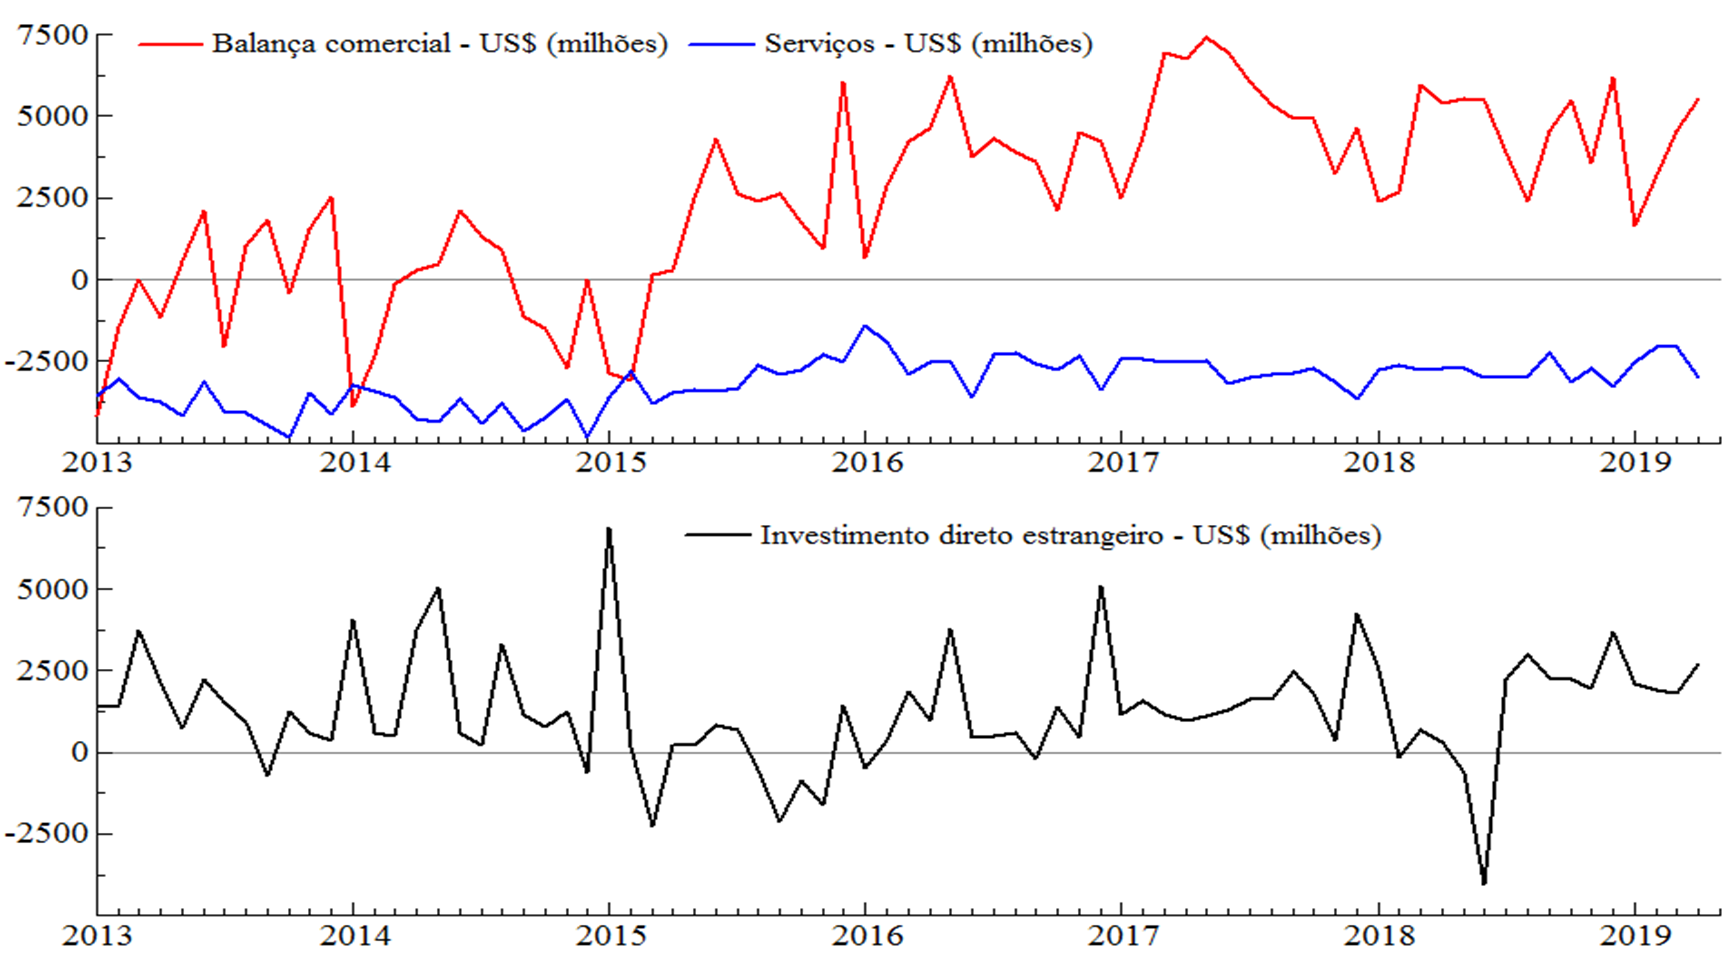
\includegraphics[width=0.7\linewidth]{Imagens/a19i1.png}
\end{figure}

\begin{figure}[H]
    \centering
    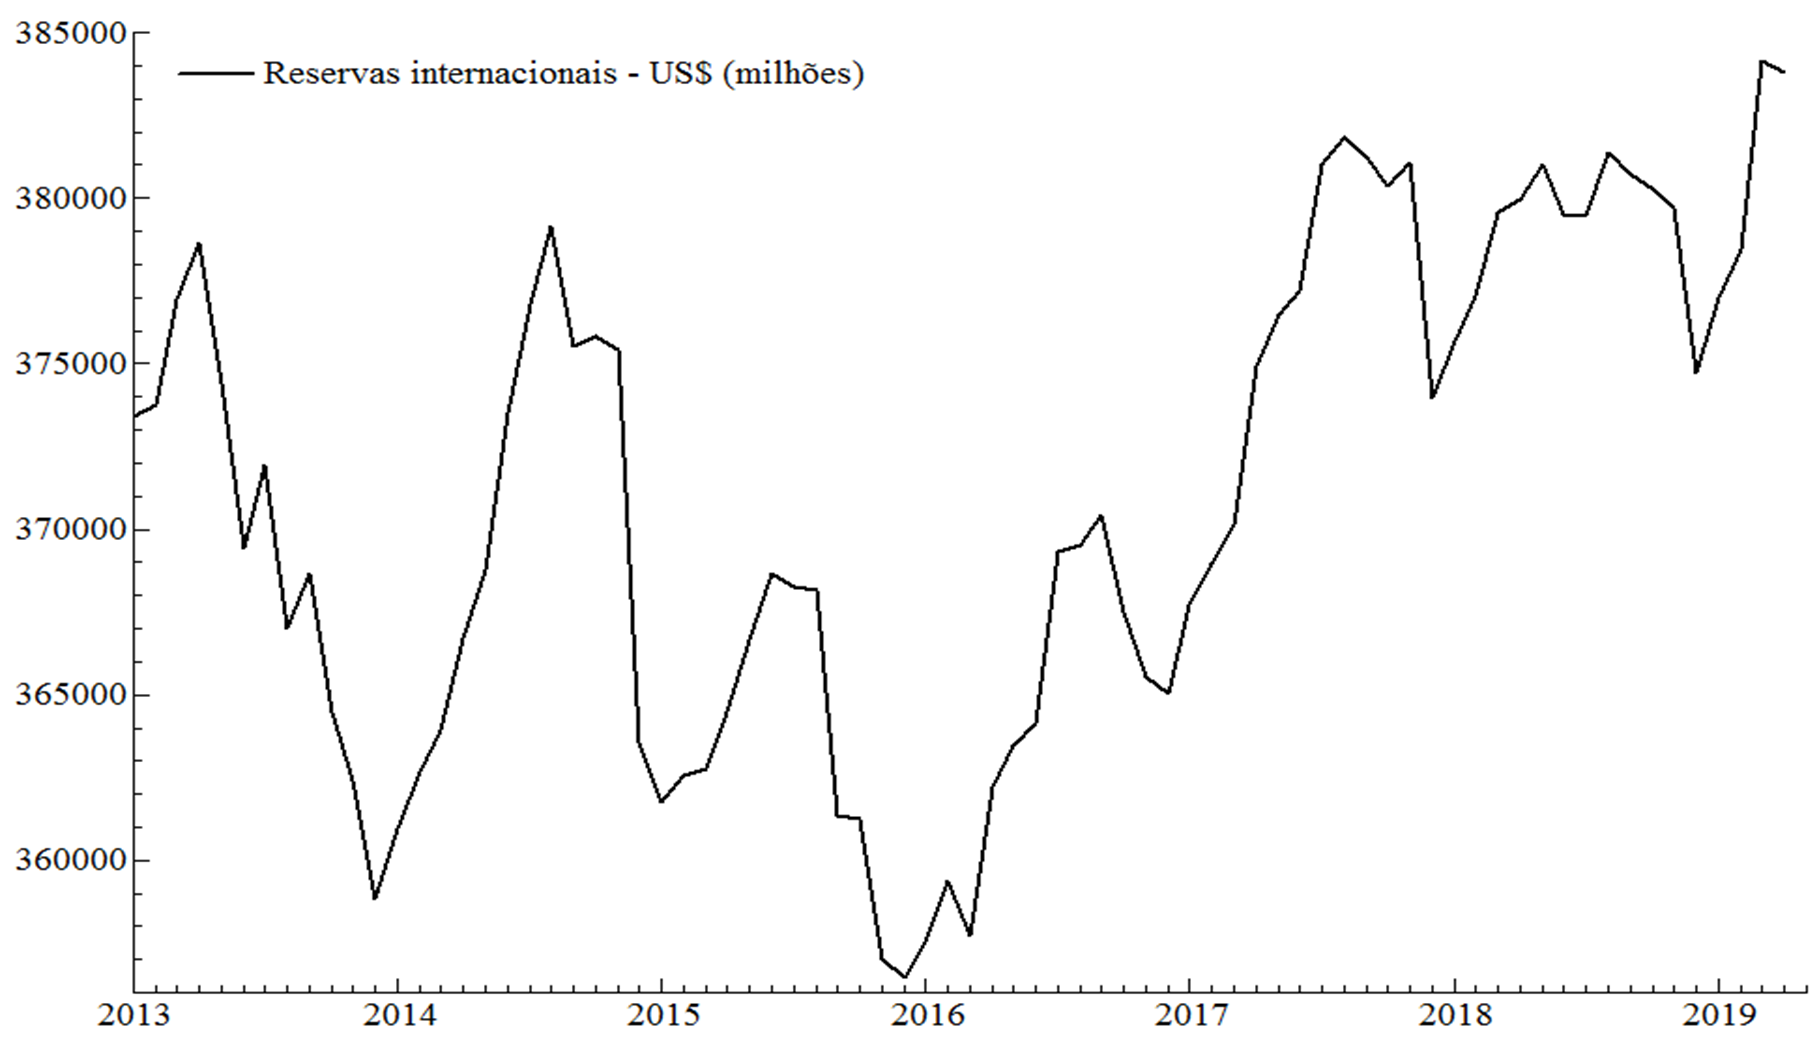
\includegraphics[width=0.7\linewidth]{Imagens/a19i2.png}
\end{figure}

\subsection{\textbf{Tendência cambial}}
\begin{figure}[H]
    \centering
    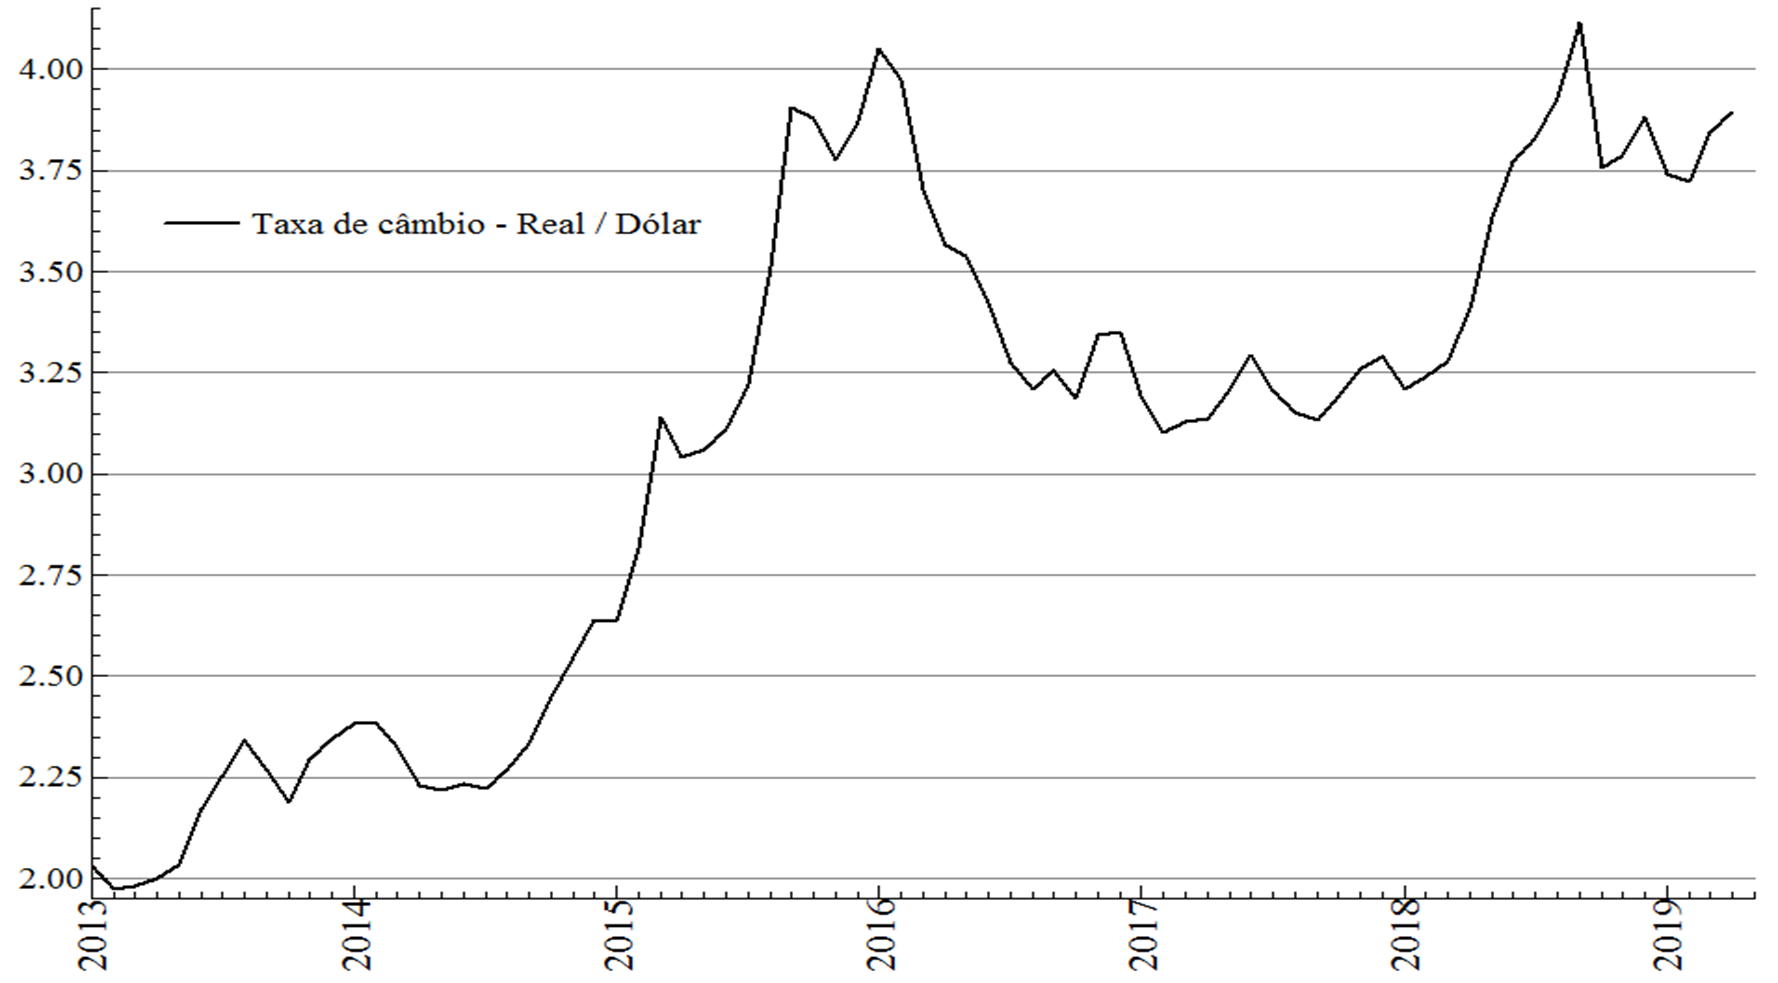
\includegraphics[width=0.7\linewidth]{Imagens/a19i3.png}
\end{figure}

\subsection{\textbf{Agenda reformista}}
A agenda reformista foi retomada, após as reformas no primeiro mandato do presidente Lula\begin{itemize}
    \item trouxe a discussão e buscou aprovar uma série de melhorias microeconômicas (mostra preocupação com a evolução da PTF);
    \item conseguiu, por exemplo, a aprovação da TLP (Taxa de longo prazo, BNDES), que busca reduzir a concessão de subsídios e dar maior transparência para as taxas de juros concedidas pelo BNDES;
    \item considerando o curto período do governo, o conjunto reformista aprovado foi significativo;
    \item provavelmente teria aprovado mais reformas, mas a crise política inviabilizou.
\end{itemize}

\subsubsection{\textbf{Reformas estruturais}}
Teto de gastos\begin{itemize}
    \item a PEC 241/55, teto de gastos, foi aprovada no final de 2016. Os gastos poderiam crescer de acordo com a inflação do ano anterior nos próximos 20 anos (seria uma “proposta Levy” suavizada);
    \item a estratégia foi “ótima” já que sinalizava compromisso com a melhoria fiscal e ao mesmo tempo a restrição mais forte seria somente em 2018;
    \item a criação de nova despesa deveria mostrar fonte de receita ou a compensação com a redução de outra despesa;
    \item mas sua sustentabilidade era fortemente dependente de uma reforma fiscal mais ampla, como as reformas da previdência e do Estado.
\end{itemize}

Reforma trabalhista (nov./2017) – “flexibilização da CLT”\begin{itemize}
    \item maior flexibilidade da regulação trabalhista tende a estimular as contratações e, portanto, reduzir o desemprego;
    \item a ideia seria elevar a segurança jurídica para empresários e trabalhadores;
    \item decisões entre a representação dos trabalhadores e a empresa empregadora não poderiam ser posteriormente contestadas na Justiça;
    \item permite também que empregados e empregadores negociem cortes nominais nos salários em eventual nova crise, preservando os postos de trabalho;
    \item teoricamente tende a gerar queda da taxa estrutural de desemprego;
    \item um recuo levaria a menores pressões inflacionárias;
    \item A efetividade desta reforma ainda é controversa.
\end{itemize}

\begin{figure}[H]
    \centering
    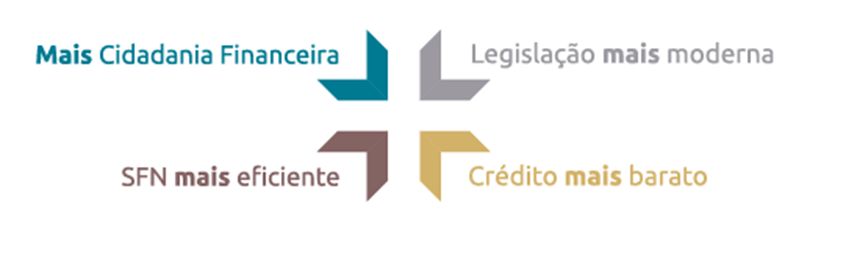
\includegraphics[width=0.7\linewidth]{Imagens/a19i4.png}
\end{figure}

Agenda BC+\begin{itemize}
    \item aumentar o nível de educação financeira. Melhorar a comunicação e a transparência entre as instituições financeiras e seus clientes;
    \item modernizar leis e normas que regem a atuação do BC. Aprimorar o modelo de relacionamento do BC com o Tesouro Nacional;
    \item simplificar os procedimentos e regras do BC;
    \item diminuir o custo do crédito para o tomador final; reduzir o nível de inadimplência; aumentar a competitividade e a flexibilidade na concessão de crédito.
\end{itemize}

\url{https://www.bcb.gov.br/acessoinformacao/bcmais}

\subsection{\textbf{Balanço do período Temer}}
Retomou regularidade na gestão de política econômica ao restabelecer o regime de metas de inflação e melhorar o lado fiscal
\begin{itemize}
    \item Inflação (IPCA foi 2,9\% e 3,75\% em 2017 e 2018, respectivamente) e os juros declinaram de forma significativa (de 14\% em 2016 para 6,5\% em 2018);
    \item a credibilidade da autoridade monetária foi retomada;
    \item melhorou a posição fiscal (déficit primário foi de 2,5\% do PIB em 2016 para 1,3\% em 2018);
    \item o Brasil saiu da recessão.
\end{itemize}

Trouxe uma agenda reformista

\subsection{\textbf{Mas...}}
Não conseguiu dar continuidade na agenda reformista já que foi perdendo o apoio político no Congresso
\begin{itemize}
    \item a reforma da previdência não passou;
    \item a recessão foi mais persistente do que se esperava e a retomada de crescimento foi fraca; (PIB avançou perto de 1\%, 2017 e 2018);
    \item reascendeu a questão “corporativista” – vide a solução para a greve dos caminhoneiros e discussão aberta sobre a política de preços da Petrobras;
    \item perdeu a janela em meados de 2018 quando chegou o momento da paralisia no Congresso com processo eleitoral;
\end{itemize}

\subsection{\textbf{UMA PONTE PARA O FUTURO}}

O programa “Uma Ponte para o Futuro” (PMDB, 29 out. 2015) foi concebido para \emph{“preservar a economia brasileira e tornar viável o seu desenvolvimento, devolvendo ao Estado a capacidade de executar políticas sociais que combatam a pobreza e criem oportunidades para todos”}.  
A seguir, apresenta-se um resumo detalhado, organizado em blocos temáticos, estritamente baseado no texto original do documento.

\subsubsection{\textbf{Diagnóstico macroeconômico e político}}
\begin{itemize}
    \item \textbf{Crise econômica}: recessão iniciada em 2014, retração do PIB, inflação e juros elevados, desemprego crescente, paralisação dos investimentos produtivos e “ausência de horizontes”.  
    \item \textbf{Crise fiscal}: déficits nominais de 6 \% (2014) e 9 \% (2015) do PIB; despesa pública crescendo acima da renda; trajetória insustentável da dívida (aprox. 70 \% do PIB, com tendência de alta).  
    \item \textbf{Riscos sociais e políticos}: estagnação econômica e esgotamento da capacidade fiscal fragilizam o pacto democrático, geram “mal-estar social” e minam a autoridade política.  
    \item \textbf{Fragmentação partidária}: sistema político “sem raízes profundas na sociedade” dificulta a construção de maiorias estáveis; o país “clama por pacificação”.
\end{itemize}

\subsubsection{\textbf{Reforma do regime fiscal e orçamentário}}
\begin{itemize}
    \item \textbf{Novo orçamento público}: elimina vinculações constitucionais (por ex., saúde e educação) e torna o orçamento \emph{impositivo}; despesas devem ser executadas salvo frustração de receita, quando se aplicaria um redutor proporcional.  
    \item \textbf{Fim das indexações}: proíbe reajustes automáticos (salário mínimo, benefícios previdenciários, salários do serviço público); cada reajuste passaria a ser deliberado no orçamento anual.  
    \item \textbf{Orçamento “base zero”}: todos os programas seriam avaliados anualmente por comitê independente, podendo ser mantidos ou encerrados conforme custo-benefício.  
    \item \textbf{Âncora constitucional}: equilíbrio fiscal de longo prazo elevado a princípio constitucional, detalhado em Lei Complementar de Responsabilidade Orçamentária.  
    \item \textbf{Autoridade Orçamentária}: órgão permanente, integrado por Executivo e Legislativo, para monitorar receitas, despesas e avaliar programas.
\end{itemize}

\subsubsection{\textbf{Reforma da previdência}}
\begin{itemize}
    \item \textbf{Déficit crescente}: diferença receitas–despesas do INSS de R\$ 82 bi (2015) e R\$ 125 bi (2016); despesa previdenciária já atinge 12 \% do PIB.  
    \item \textbf{Medidas propostas}: 
    \begin{itemize}
        \item introduzir idade mínima progressiva (65 anos homens, 60 anos mulheres, com futuras elevações);  
        \item eliminar indexação de benefícios ao salário mínimo, mantendo apenas a reposição inflacionária;  
        \item preservar direitos adquiridos, com transição para quem está próximo de se aposentar.
    \end{itemize}
\end{itemize}

\subsubsection{\textbf{Juros, dívida e política monetária}}
\begin{itemize}
    \item \textbf{Custo da dívida}: serviço da dívida pública próximo de 8 \% do PIB em 2015, sobretudo devido a juros nominais de 14 \%.  
    \item \textbf{Objetivo}: alcançar superávit primário suficiente para estabilizar e, depois, reduzir a relação dívida/PIB; queda sustentável da inflação permitiria reduzir a taxa básica de juros.  
    \item \textbf{Dívida de curto prazo}: quase 40 \% do estoque em financiamento diário (LFTs e compromissadas); meta de alongar prazos gradualmente após consolidação fiscal.  
    \item \textbf{Swaps cambiais}: custo potencial de ~2 \% do PIB em 2015; defende-se debate público sobre limites e governança dessas operações.
\end{itemize}

\subsubsection{\textbf{Agenda de crescimento e inserção internacional}}
\begin{itemize}
    \item \textbf{Meta de longo prazo}: crescer 3,5–4 \% ao ano (PIB) para elevar a renda per capita em 2,5 \% ao ano na próxima década.  
    \item \textbf{Motor do ciclo}: investimento privado, ganhos de produtividade e competitividade externa (agronegócio e indústria).  
    \item \textbf{Infraestrutura}: ampliação de concessões, parcerias e transferências de ativos, com realismo tarifário.  
    \item \textbf{Abertura comercial}: buscar acordos regionais com EUA, UE e Ásia; remover barreiras, convergir normas e integrar cadeias globais de valor — com ou sem o Mercosul (preferencialmente com).  
    \item \textbf{Governança pública}: regras estritas de nomeação e responsabilização para estatais e agências reguladoras; fortalecimento da segurança jurídica.  
    \item \textbf{Ambiente de negócios}: simplificação tributária (unificação ICMS, desoneração de exportações e investimentos), racionalização burocrática e licenças ambientais mais céleres.  
    \item \textbf{Inovação e P\&D}: alta prioridade a pesquisa, desenvolvimento tecnológico e educação.
\end{itemize}

\subsubsection{\textbf{Pontos estruturantes (a–l) destacados pelo documento}}
\begin{enumerate}
    \item Trajetória estável de superávit operacional e queda da dívida.  
    \item Limite para despesas de custeio abaixo do crescimento do PIB.  
    \item Estabilizar dívida/PIB e inflação na meta em até 3 anos, permitindo juros reais internacionais.  
    \item Política de desenvolvimento centrada na iniciativa privada (concessões, partilha, TLP).  
    \item Inserção plena no comércio internacional via acordos regionais e abertura comercial.  
    \item Governança corporativa avançada em estatais e reguladoras.  
    \item Reforma do processo orçamentário para gasto transparente e eficiente.  
    \item Agenda de avaliação de políticas públicas, identificando beneficiários e impactos.  
    \item Prevalência de convenções coletivas sobre legislação trabalhista, salvo direitos básicos.  
    \item Simplificação tributária ampla: menos impostos e legislação ICMS unificada.  
    \item Racionalização burocrática, segurança jurídica e licenciamento ambiental ágil.  
    \item Prioridade à pesquisa, desenvolvimento tecnológico e inovação.
\end{enumerate}

\subsubsection{\textbf{Conexão com o governo Temer (2016–2018)}}
\begin{itemize}
    \item Várias propostas do documento se materializaram: Teto de Gastos (PEC 241/55), reforma trabalhista, TLP, agenda BC+, reequilíbrio fiscal parcial e retomada da credibilidade monetária.  
    \item Outros pontos ficaram incompletos: reforma da previdência não aprovada; abertura comercial limitada; avanço modesto na simplificação tributária e na reforma do Estado.  
    \item O programa serviu, portanto, como \emph{roteiro} conceitual para a política econômica do período Temer, embora nem todas as medidas tenham logrado apoio político suficiente para implementação integral.
\end{itemize}


\newpage
\section{\textbf{Resolvendo o Guia de Questões}}
\subsection{\textbf{1º Guia}}
\subsubsection{\textbf{Considerando as múltiplas funções do Banco do Brasil na década de 1950: por que havia uma tendência de acelerar a inflação?}}

A tendência de aceleração inflacionária na década de 1950, em especial no contexto do Plano de Metas do governo Juscelino Kubitschek, está fortemente relacionada ao papel multifuncional do Banco do Brasil (BB) dentro do Sistema Financeiro Brasileiro (SFB) da época. O BB atuava simultaneamente como banco comercial e como agente de política econômica do governo, o que gerava sérios conflitos com a condução de uma política monetária restritiva. A seguir, destacam-se os principais fatores que explicam essa tendência:

\begin{itemize}
    \item \textbf{Vazamentos da política monetária:} 
    Dois canais principais permitiam a expansão da base monetária:
    \begin{enumerate}
        \item \textit{Emissão de papel-moeda:} Embora a emissão fosse feita formalmente pela Caixa de Amortização, o BB tinha o poder de colocar essa moeda em circulação, frequentemente por meio de concessão de crédito subsidiado ao setor agrícola, industrial ou mesmo a pessoas físicas.
        \item \textit{Transformação de moeda escritural em base monetária:} O BB, ao acolher os depósitos compulsórios dos demais bancos, podia expandir crédito de forma praticamente ilimitada, funcionando como criador autônomo de moeda.
    \end{enumerate}

    \item \textbf{Pressões políticas e sociais:} O Congresso Nacional, pressionado por diferentes grupos de interesse, frequentemente ampliava os limites de financiamento do BB, agravando a expansão monetária. O banco não era um agente irracional, mas sim instrumento de um sistema político-econômico no qual diversos atores demandavam continuamente crédito subsidiado.

    \item \textbf{Financiamento do Plano de Metas:} Os recursos necessários para a execução do plano vinham, em boa parte, de uma ``poupança forçada'' via inflação. Ou seja, o aumento da emissão monetária permitia financiar investimentos públicos e privados estratégicos, mesmo sem o correspondente aumento da arrecadação fiscal.

    \item \textbf{Instituições extrativistas:} De acordo com a interpretação de Acemoglu e Robinson, o modelo institucional vigente no Brasil era extrativista, favorecendo grupos específicos com acesso privilegiado a crédito e subsídios, em detrimento do equilíbrio macroeconômico de longo prazo.
\end{itemize}

Em síntese, a atuação do Banco do Brasil como elo entre a política monetária e os interesses do governo e da sociedade organizada produziu vazamentos monetários difíceis de conter. Isso estruturou uma dinâmica inflacionária persistente, que financiava o crescimento mas ao custo de graves desequilíbrios macroeconômicos.

\subsubsection{\textbf{Como podemos caracterizar o Plano de Metas? Quais foram as consequências produtivas e macroeconômicas a partir desse plano?}}

O Plano de Metas (1957--1961), conduzido durante o governo de Juscelino Kubitschek, pode ser caracterizado como uma estratégia de crescimento econômico baseada na industrialização acelerada, com forte protagonismo do Estado e articulação com o setor privado e o capital estrangeiro. Inspirado pelo pensamento estruturalista da CEPAL, o plano adotou uma lógica de substituição de importações (PSI) com foco em setores estratégicos.

\begin{itemize}
    \item \textbf{Características principais:}
    \begin{enumerate}
        \item \textit{Planejamento centralizado:} Elaboração de 30 metas distribuídas em cinco grandes áreas: energia, transporte, indústrias de base, alimentação e educação; além da construção de Brasília.
        \item \textit{Participação estatal:} O Estado liderou os investimentos por meio do Banco do Brasil, BNDE e Tesouro Nacional.
        \item \textit{Escolha de setores estratégicos:} Forte estímulo à indústria automobilística, construção naval e equipamentos elétricos, com subsídios, proteção tarifária e crédito direcionado.
        \item \textit{Articulação institucional:} Criação do Conselho de Desenvolvimento e do Conselho de Política Aduaneira; adoção da Lei do Similar Nacional e da Regra de Conteúdo Local (RCL).
    \end{enumerate}

    \item \textbf{Consequências produtivas:}
    \begin{itemize}
        \item Modernização da indústria nacional, com destaque para a consolidação da cadeia automobilística e de autopeças.
        \item Expansão da infraestrutura logística e energética.
        \item Nacionalização produtiva de setores até então fortemente dependentes de importações.
        \item Atração de Investimento Direto Estrangeiro (IDE) e urbanização acelerada.
    \end{itemize}

    \item \textbf{Consequências macroeconômicas:}
    \begin{itemize}
        \item \textit{Inflação crescente:} Resultado da “poupança forçada” viabilizada por emissão monetária, principalmente via Banco do Brasil.
        \item \textit{Desequilíbrio fiscal e externo:} A expansão dos gastos públicos e das importações pressionou as contas públicas e o balanço de pagamentos.
        \item \textit{Instituições extrativistas:} O modelo reforçou a concessão de benefícios seletivos a grupos específicos (via crédito, subsídios e proteção), em detrimento de medidas horizontais e universais.
        \item \textit{Crescimento com prazo de validade:} Apesar do forte dinamismo produtivo, os desequilíbrios acumulados geraram instabilidade e crises no início da década de 1960.
    \end{itemize}
\end{itemize}

Em síntese, o Plano de Metas representou um impulso significativo ao processo de industrialização brasileira, com ganhos estruturais importantes. No entanto, sua condução verticalizada e dependente de financiamento inflacionário comprometeu a sustentabilidade macroeconômica, contribuindo para a crise que se seguiu nos anos posteriores.

\subsubsection{\textbf{Explique o Plano Trienal (1962): qual era seu diagnóstico para a aceleração inflacionária? Quais foram as consequências a partir de suas medidas?}}

O Plano Trienal de Desenvolvimento Econômico e Social, lançado no final de 1962 sob coordenação de Celso Furtado durante o governo de João Goulart (Jango), representou uma tentativa de estabilização gradual da economia brasileira, conciliando crescimento com controle inflacionário e reformas sociais.

\begin{itemize}
    \item \textbf{Diagnóstico da inflação:}
    \begin{itemize}
        \item A inflação era vista como resultado da forte expansão dos gastos públicos nos anos anteriores, especialmente durante o governo JK.
        \item O diagnóstico combinava elementos ortodoxos (déficit fiscal como causa da inflação) e heterodoxos (necessidade de reformas estruturais para lidar com os gargalos de oferta).
        \item Reconhecia também a existência de expectativas inflacionárias e mecanismos de indexação que perpetuavam o processo inflacionário.
    \end{itemize}

    \item \textbf{Medidas propostas:}
    \begin{enumerate}
        \item \textit{Controle fiscal:} Contenção de gastos públicos e aumento de receitas, buscando o equilíbrio orçamentário.
        \item \textit{Política monetária restritiva:} Limitação à expansão do crédito, com medidas específicas como as Instruções 234 (para o BB) e 235 (para bancos privados), que restringiam a concessão de crédito.
        \item \textit{Política cambial realista:} Redução dos subsídios às importações e desvalorização cambial gradual.
        \item \textit{Política salarial racionalizada:} Tentativas de compatibilizar reajustes salariais com ganhos de produtividade.
        \item \textit{Congelamento de preços seletivo:} Acordos pontuais com setores empresariais para conter aumentos de preços (medida heterodoxa).
    \end{enumerate}

    \item \textbf{Consequências do plano:}
    \begin{itemize}
        \item \textit{Resistência política:} Medidas ortodoxas enfrentaram oposição tanto de sindicatos (pela perda salarial) quanto de setores empresariais (pela retirada de subsídios).
        \item \textit{Reação dos agentes:} Expectativa de congelamento levou a aumentos preventivos de preços, agravando a inflação no curto prazo.
        \item \textit{Inconsistência interna:} O plano combinava metas conflitantes — combate à inflação e crescimento de 7\% ao ano — o que gerou descrença na sua viabilidade.
        \item \textit{Fracasso e abandono:} Em maio de 1963, o plano começou a ser abandonado. Jango passou a apoiar aumentos salariais, rompendo com o espírito de estabilização.
        \item \textit{Recessão de 1963:} A economia entrou em retração, com desaceleração do PIB e alta inflação. Explicações variam entre esgotamento da PSI (Furtado e Tavares), turbulência política (Simonsen) e sequência de medidas sem resultados (Mesquita).
    \end{itemize}

    \item \textbf{Síntese:}
    O Plano Trienal foi uma tentativa sofisticada de compatibilizar estabilização e desenvolvimento, porém esbarrou nas limitações políticas do governo Jango, na reação adversa dos agentes econômicos e na fragilidade institucional do período. A recessão de 1963 e a aceleração inflacionária subsequente marcaram o fracasso da estratégia, reforçando a leitura de que as instituições brasileiras mantinham traços extrativistas, conforme o referencial de Acemoglu e Robinson.
\end{itemize}

\subsubsection{\textbf{Quais são as principais explicações para entendermos a recessão de 1963/64? Como podemos criticar essas explicações?}}

A recessão de 1963/64 — a primeira desde 1943 — é objeto de múltiplas interpretações que buscam explicar suas causas a partir de diferentes abordagens. As principais explicações podem ser agrupadas em três vertentes:

\begin{itemize}
    \item \textbf{1. Esgotamento da Política de Substituição de Importações (PSI):}
    \begin{itemize}
        \item Defendida por autores como Celso Furtado e Maria da Conceição Tavares.
        \item Argumenta que o modelo de industrialização baseado na substituição de importações havia alcançado seus limites estruturais.
        \item Destaca gargalos no setor externo e dificuldades em ampliar o mercado interno sem gerar pressões inflacionárias e desequilíbrios cambiais.
    \end{itemize}
    \textit{Crítica:} Apesar de coerente, a hipótese do esgotamento estrutural não explica a intensidade da recessão no curto prazo. Além disso, desconsidera o papel das escolhas de política econômica e do ambiente político conturbado.

    \item \textbf{2. Aceleração inflacionária e incerteza (Simonsen):}
    \begin{itemize}
        \item Inspirado na lógica monetarista, argumenta que a inflação crescente gerou incerteza nos agentes econômicos, inibindo investimentos e consumo.
        \item A instabilidade política desde 1961, com rutura institucional e mudanças no regime de governo, ampliou a incerteza.
    \end{itemize}
    \textit{Crítica:} Embora a incerteza inflacionária e política seja relevante, a tese peca por reduzir o problema a um choque de expectativas, sem considerar os fatores estruturais e a complexidade institucional do período.

    \item \textbf{3. Sequência de planos de estabilização com custos concentrados (Mesquita):}
    \begin{itemize}
        \item Argumenta que o Brasil testou várias estratégias de estabilização (Quadros, Jango), mas sem resultados claros no curto prazo.
        \item Os custos (redução da demanda, queda salarial, escassez de crédito) foram sentidos de imediato, enquanto os ganhos não se concretizaram.
        \item Isso reduziu a confiança dos empresários e afastou o investimento estrangeiro.
    \end{itemize}
    \textit{Crítica:} Essa abordagem é eficaz em descrever o ambiente econômico imediato, mas não explora suficientemente os condicionantes políticos e institucionais que inviabilizaram a coordenação de políticas.

    \item \textbf{4. Interpretação institucional:}
    \begin{itemize}
        \item Segundo a perspectiva de Acemoglu e Robinson, a recessão pode ser explicada pelo funcionamento de \textit{instituições extrativistas}, que favoreciam grupos específicos em detrimento da estabilidade macroeconômica.
        \item A ausência de instituições inclusivas e de uma coalizão política estável inviabilizou a implementação eficaz de qualquer plano de estabilização.
    \end{itemize}
    \textit{Contribuição:} Essa leitura oferece uma crítica de fundo às demais explicações, ao ressaltar que a fragilidade institucional brasileira — marcada por desigualdade, patrimonialismo e captura do Estado — limitava sistematicamente a eficácia das políticas econômicas.
\end{itemize}

\textbf{Síntese:} As explicações tradicionais — esgotamento do modelo, aceleração inflacionária, instabilidade política — ajudam a compreender elementos específicos da recessão de 1963/64. No entanto, uma análise mais robusta exige incorporar a dimensão institucional, que evidencia os limites estruturais do Estado brasileiro para coordenar políticas de estabilização em um ambiente de intensa disputa distributiva e baixa legitimidade.

\subsubsection{\textbf{Explicar as principais reformas estruturais propostas no PAEG e quais foram suas consequências de médio e longo prazos para a economia brasileira.}}

O Programa de Ação Econômica do Governo (PAEG), implementado entre 1964 e 1966 sob liderança do ministro Roberto Campos, representou uma resposta à crise de estagflação herdada do período anterior. O plano combinou políticas de estabilização gradual com um ambicioso conjunto de reformas estruturais, que moldaram o funcionamento da economia brasileira nas décadas seguintes.

\begin{itemize}
    \item \textbf{1. Reforma Tributária}
    \begin{itemize}
        \item \textit{Objetivo:} Ampliar a arrecadação e racionalizar o sistema tributário.
        \item \textit{Medidas principais:}
        \begin{itemize}
            \item Criação do ICM (Imposto sobre Circulação de Mercadorias) e do ISS (Imposto Sobre Serviços).
            \item Ampliação da base do Imposto de Renda.
            \item Extinção de tributos ineficientes e modernização da arrecadação via rede bancária.
        \end{itemize}
        \item \textit{Consequências:}
        \begin{itemize}
            \item A carga tributária aumentou de 16\% para 21\% do PIB (1963–1967).
            \item Estrutura regressiva, com ênfase em tributos indiretos, impactando negativamente a distribuição de renda.
            \item Centralização do poder fiscal na União, via FPEM, reduzindo a autonomia de estados e municípios.
        \end{itemize}
    \end{itemize}

    \item \textbf{2. Reforma Financeira}
    \begin{itemize}
        \item \textit{Objetivo:} Modernizar o sistema bancário e criar condições para o financiamento de longo prazo.
        \item \textit{Medidas principais:}
        \begin{itemize}
            \item Criação do Banco Central do Brasil e do Conselho Monetário Nacional.
            \item Expansão dos bancos de investimento e do mercado de capitais.
            \item Introdução da correção monetária (ORTN) para títulos públicos e contratos.
        \end{itemize}
        \item \textit{Consequências:}
        \begin{itemize}
            \item Consolidação de um sistema financeiro mais estruturado, com maior capacidade de intermediação.
            \item Viabilização do financiamento habitacional (via SFH) e de grandes investimentos.
            \item Institucionalização da indexação, com efeitos ambíguos: inicialmente reduziu a incerteza, mas consolidou a inflação inercial.
        \end{itemize}
    \end{itemize}

    \item \textbf{3. Reforma do Mercado de Trabalho}
    \begin{itemize}
        \item \textit{Objetivo:} Aumentar a flexibilidade do mercado de trabalho e reduzir os custos para os empregadores.
        \item \textit{Medida principal:} Criação do Fundo de Garantia por Tempo de Serviço (FGTS), em substituição à estabilidade decenal.
        \item \textit{Consequências:}
        \begin{itemize}
            \item Maior dinamismo no mercado de trabalho, com estímulo à contratação.
            \item Redução da proteção ao trabalhador e enfraquecimento do poder sindical.
            \item Utilização do FGTS como instrumento de financiamento habitacional e de infraestrutura.
        \end{itemize}
    \end{itemize}

    \item \textbf{4. Reforma Salarial}
    \begin{itemize}
        \item \textit{Objetivo:} Controlar a inflação de custos por meio de regras rígidas de reajuste salarial.
        \item \textit{Medidas principais:}
        \begin{itemize}
            \item Reajuste anual com base em inflação passada e crescimento da produtividade.
            \item Eliminação da negociação coletiva como principal forma de reajuste.
        \end{itemize}
        \item \textit{Consequências:}
        \begin{itemize}
            \item Queda real dos salários ao longo da década de 1960.
            \item Redução da parcela do trabalho na renda nacional.
            \item Contribuição para o sucesso da estabilização, mas com aumento da desigualdade.
        \end{itemize}
    \end{itemize}
\end{itemize}

\textbf{Síntese:} O PAEG promoveu um redesenho profundo das instituições econômicas brasileiras. No médio prazo, contribuiu para a estabilização monetária e para a retomada do crescimento — viabilizando, inclusive, o chamado “milagre econômico” a partir de 1968. No entanto, os custos sociais foram significativos, com aumento da desigualdade, enfraquecimento da negociação trabalhista e institucionalização de mecanismos que dificultariam o combate à inflação no longo prazo, como a indexação generalizada.

\subsubsection{\textbf{Como podemos estabelecer relações entre o Milagre econômico e: a taxa de inflação, o setor externo e a industrialização?}}

O período do “Milagre Econômico” brasileiro (1968–1973) foi marcado por altas taxas de crescimento do PIB (média de 11,2\% ao ano), combinadas com inflação relativamente controlada e fortalecimento da industrialização. Esse desempenho excepcional foi sustentado por um conjunto coordenado de políticas econômicas e institucionais, articulando política monetária expansionista, estímulo ao investimento e um ambiente externo favorável. As relações com os três pilares mencionados podem ser descritas da seguinte forma:

\begin{itemize}
    \item \textbf{1. Inflação}
    \begin{itemize}
        \item \textit{Diagnóstico dominante:} A inflação era vista como “de custos”, especialmente atribuída ao alto custo do crédito.
        \item \textit{Política de contenção:}
        \begin{itemize}
            \item Concessão de crédito subsidiado ao setor agrícola e industrial.
            \item Criação do Orçamento Monetário, que segregava despesas financeiras e mascarava a verdadeira expansão fiscal.
            \item Políticas de controle direto de preços, via o CIP (Conselho Interministerial de Preços), que congelava reajustes de preços públicos e privados com base em planilhas de custos.
            \item Política salarial de arrocho (derretimento real dos salários), persistente desde o PAEG.
        \end{itemize}
        \item \textit{Resultado:} Apesar da forte expansão da demanda e do crédito, a inflação permaneceu em trajetória declinante, graças ao controle de preços, capacidade ociosa da economia e entrada de capitais externos.
    \end{itemize}

    \item \textbf{2. Setor Externo}
    \begin{itemize}
        \item \textit{Balança comercial:} Houve expansão simultânea das exportações (favorecidas por incentivos fiscais e cambiais) e das importações (insumos para a industrialização), mantendo a balança comercial relativamente equilibrada.
        \item \textit{Conta de capitais (CK):} Superavitária, sustentada pela entrada de Investimento Direto Estrangeiro (IDE) e pela formação do mercado de eurodólares, com juros internacionais baixos.
        \item \textit{Política cambial:} Adoção do regime de \textit{crawling peg} (minidesvalorizações cambiais periódicas), para preservar a competitividade externa e compensar a inflação interna.
        \item \textit{Resultado:} Forte acúmulo de reservas internacionais e equilíbrio do balanço de pagamentos, o que sustentou a estabilidade macroeconômica do período.
    \end{itemize}

    \item \textbf{3. Industrialização}
    \begin{itemize}
        \item \textit{Políticas setoriais ativas:}
        \begin{itemize}
            \item Fortes subsídios para setores estratégicos (autopeças, eletrodomésticos, máquinas e equipamentos).
            \item Incentivos ao setor exportador (têxteis, calçados, alimentos industrializados).
            \item Ampliação do crédito via sociedades de crédito e investimentos, promovendo o consumo de bens duráveis.
        \end{itemize}
        \item \textit{PED – Plano Estratégico de Desenvolvimento (1968):}
        \begin{itemize}
            \item Estímulo à indústria de bens de capital e bens intermediários (siderurgia, metalurgia).
            \item Expansão da linha branca (geladeira, fogão, TV), ligada ao processo de urbanização.
        \end{itemize}
        \item \textit{Resultado:} Fortalecimento da estrutura produtiva nacional, elevação da produtividade e diversificação do parque industrial.
    \end{itemize}
\end{itemize}

\textbf{Síntese:} O Milagre Econômico resultou de uma convergência entre ambiente externo favorável, políticas industriais seletivas, repressão salarial e controle de preços. Essa articulação permitiu combinar crescimento acelerado com inflação sob controle, saldo externo positivo e avanços significativos na industrialização. No entanto, o modelo dependia de fatores conjunturais não sustentáveis (juros baixos, abundância de capital externo, controle autoritário), e seu esgotamento tornou-se evidente após o primeiro choque do petróleo (1973).

\subsubsection{\textbf{Como o Presidente Geisel reagiu diante do 1º choque do Petróleo em 1973? Quais foram as consequências para a economia brasileira a partir dessa reação?}}

O presidente Ernesto Geisel assumiu o governo em 1974, em meio aos efeitos do 1º choque do petróleo (1973), que elevou bruscamente o preço do barril e agravou a vulnerabilidade externa de economias dependentes da importação de energia, como o Brasil. Diante desse cenário, Geisel optou por uma estratégia não recessiva, priorizando a manutenção do crescimento via aumento da capacidade produtiva e substituição de importações. Essa decisão resultou na formulação e execução do \textbf{II Plano Nacional de Desenvolvimento (II PND)}.

\begin{itemize}
    \item \textbf{Reação ao choque: principais decisões}
    \begin{itemize}
        \item \textit{Rejeição do ajuste recessivo:} Apesar das pressões inflacionárias e do desequilíbrio externo, Geisel evitou políticas ortodoxas de retração da demanda, por temer os custos políticos e sociais.
        \item \textit{Adoção de uma estratégia estruturalista de longo prazo:} Lançamento do II PND (1974--1979), que visava transformar a estrutura produtiva do país para reduzir a dependência de bens importados e de petróleo.
        \item \textit{Financiamento externo:} A estratégia baseou-se em endividamento externo em um contexto de abundância de crédito internacional (petrodólares), com juros ainda baixos.
    \end{itemize}

    \item \textbf{Instrumentos e áreas prioritárias do II PND}
    \begin{itemize}
        \item \textit{Infraestrutura:} Expansão da malha ferroviária, hidroelétrica e do setor de telecomunicações.
        \item \textit{Indústria pesada:} Fortes investimentos em bens de capital, aço, alumínio, petroquímica, fertilizantes e papel e celulose.
        \item \textit{Setor energético:} Ampliação da produção nacional de petróleo (Bacia de Campos), desenvolvimento da energia hidroelétrica (Itaipu, Tucuruí) e incentivo à energia alternativa (etanol, nuclear).
        \item \textit{Política industrial e tecnológica:} Incentivos fiscais, crédito subsidiado, proteção via tarifas e reservas de mercado.
    \end{itemize}

    \item \textbf{Consequências econômicas}
    \begin{itemize}
        \item \textit{Crescimento econômico:} O PIB manteve taxas elevadas (média de 7\% ao ano), com expansão da capacidade produtiva e da base industrial.
        \item \textit{Redução da dependência de insumos estratégicos:} Queda nominal nas importações de bens básicos e aumento da produção nacional de insumos industriais.
        \item \textit{Aumento do endividamento externo:} A dívida externa brasileira passou de US\$ 12,5 bilhões (1974) para mais de US\$ 21 bilhões (1978), e os encargos com juros aumentaram rapidamente.
        \item \textit{Desequilíbrio fiscal:} A expansão dos gastos públicos e dos subsídios comprometeu a posição fiscal do Estado.
        \item \textit{Pressão inflacionária:} Apesar das tentativas de controle, a inflação voltou a crescer na segunda metade da década, pressionada pelo excesso de demanda e pelos efeitos dos choques externos subsequentes.
    \end{itemize}

    \item \textbf{Avaliação crítica}
    \begin{itemize}
        \item \textit{Avanços:} O plano gerou ganhos produtivos e estruturais, como a diversificação da base industrial, redução das importações estratégicas e fortalecimento do setor energético.
        \item \textit{Limites:} O modelo baseava-se em protecionismo, subsídios e dívida externa crescente — pilares insustentáveis no longo prazo.
        \item \textit{Legado:} O sucesso de curto prazo gerou passivos que se materializaram na crise da dívida, inflação elevada e colapso do modelo na década de 1980.
    \end{itemize}
\end{itemize}

\textbf{Síntese:} A reação de Geisel ao 1º choque do petróleo privilegiou o crescimento com endividamento, evitando medidas recessivas e apostando na substituição de importações. Embora tenha gerado avanços industriais e energéticos, o custo foi uma deterioração fiscal e externa, que culminou na chamada “década perdida” nos anos seguintes.

\subsubsection{\textbf{Como podemos caracterizar o II PND? Quais eram seus objetivos? E quais foram as consequências?}}

O II Plano Nacional de Desenvolvimento (II PND), implementado entre 1974 e 1979 no governo Ernesto Geisel, foi a principal resposta da política econômica brasileira ao 1º choque do petróleo (1973). Inserido em um contexto de crescimento com restrições externas, o plano buscava preservar o dinamismo econômico sem recorrer a um ajuste recessivo. Foi uma estratégia estruturalista, fortemente intervencionista, baseada em planejamento estatal, endividamento externo e políticas industriais seletivas.

\begin{itemize}
    \item \textbf{Caracterização do plano:}
    \begin{itemize}
        \item Plano de longo prazo, com foco na transformação estrutural da economia.
        \item Priorizava setores estratégicos: bens de capital, insumos básicos e energia.
        \item Manteve a lógica da substituição de importações, mas agora em setores mais sofisticados.
        \item Fortemente financiado por crédito externo, com participação ativa do Estado e das estatais.
    \end{itemize}

    \item \textbf{Objetivos principais:}
    \begin{enumerate}
        \item \textit{Reduzir a vulnerabilidade externa} ao petróleo e a insumos industriais importados.
        \item \textit{Expandir a infraestrutura energética e logística}, garantindo base para o crescimento.
        \item \textit{Fortalecer a capacidade industrial nacional} em áreas de alta intensidade de capital e tecnologia.
        \item \textit{Manter taxas elevadas de crescimento econômico}, mesmo diante do cenário internacional adverso.
    \end{enumerate}

    \item \textbf{Instrumentos utilizados:}
    \begin{itemize}
        \item Incentivos fiscais e crédito subsidiado (via BNDE).
        \item Reserva de mercado e proteção tarifária.
        \item Participação ativa das estatais nos setores estratégicos.
        \item Captação de financiamento externo (petrodólares).
    \end{itemize}

    \item \textbf{Consequências:}
    \begin{itemize}
        \item \textit{Produtivas e estruturais:}
        \begin{itemize}
            \item Expansão da infraestrutura energética (hidrelétricas, Itaipu, Bacia de Campos, Nuclebrás).
            \item Desenvolvimento da indústria pesada e de bens de capital.
            \item Redução da participação dos bens de capital importados nos investimentos nacionais.
            \item Fortalecimento da base exportadora industrial.
        \end{itemize}
        
        \item \textit{Macroeconômicas:}
        \begin{itemize}
            \item Forte aumento do endividamento externo (US\$ 12,5 bi em 1974 → US\$ 21 bi em 1978).
            \item Pressão inflacionária crescente e deterioração fiscal.
            \item Fragilidade estrutural do setor público devido aos subsídios e desonerações.
            \item Sustentação do crescimento a curto prazo, mas com altos custos de médio e longo prazo.
        \end{itemize}

        \item \textit{Crítica e legado:}
        \begin{itemize}
            \item Embora tenha gerado ganhos estruturais, o modelo foi financeiramente insustentável.
            \item Criou as condições para a crise da dívida e a “década perdida” nos anos 1980.
            \item Reforçou práticas extrativistas, com benefícios concentrados e sem contrapartidas produtivas universais.
        \end{itemize}
    \end{itemize}
\end{itemize}

\textbf{Síntese:} O II PND foi um ambicioso plano de industrialização via endividamento externo, que garantiu crescimento e avanços estruturais no curto prazo, mas comprometeu a sustentabilidade macroeconômica do país no longo prazo, deixando como herança uma economia altamente endividada, indexada e desigual.

\subsubsection{\textbf{Como podemos explicar o início da recessão em 1981?}}

O início da recessão em 1981 marcou uma inflexão no ciclo de crescimento iniciado nos anos 1970 e é considerado o ponto de partida da chamada “década perdida” da economia brasileira. A recessão resultou da convergência de choques externos adversos, esgotamento do modelo de crescimento com endividamento e da mudança de orientação da política econômica no governo Figueiredo.

\begin{itemize}
    \item \textbf{1. Contexto internacional adverso:}
    \begin{itemize}
        \item \textit{2º choque do petróleo (1979):} Elevou novamente os preços do petróleo, pressionando a balança comercial brasileira.
        \item \textit{Aumento dos juros internacionais:} A política monetária restritiva dos EUA (Volcker shock) elevou os juros, encarecendo o serviço da dívida externa.
        \item \textit{Desaceleração do comércio global:} Reduziu a demanda por exportações brasileiras, agravando a restrição externa.
    \end{itemize}

    \item \textbf{2. Esgotamento do modelo de crescimento com endividamento:}
    \begin{itemize}
        \item A estratégia adotada desde o II PND baseava-se na expansão do investimento público e no financiamento externo.
        \item O crescimento do serviço da dívida tornou esse modelo insustentável: os pagamentos de juros passaram de US\$ 600 milhões (1974) para mais de US\$ 4 bilhões em
    \end{itemize}
\end{itemize}

\subsubsection{\textbf{Explicar o processo de ajustamento do setor externo brasileiro ao longo da primeira metade da década de 1980.}}

O ajustamento do setor externo brasileiro entre 1981 e 1985 ocorreu em resposta à grave crise da dívida externa e à deterioração do balanço de pagamentos. O objetivo central era gerar superávits comerciais suficientes para garantir o pagamento do serviço da dívida externa e restaurar a credibilidade internacional do país. Esse processo foi marcado por políticas recessivas, desvalorização cambial e controle do consumo interno.

\begin{itemize}
    \item \textbf{1. Contexto da crise}
    \begin{itemize}
        \item O Brasil entrou nos anos 1980 com alto nível de endividamento externo (US\$ 80 bilhões em 1982) e crescente dificuldade de rolagem.
        \item A elevação abrupta das taxas de juros internacionais, provocada pela política do Fed (Volcker), aumentou drasticamente o custo do serviço da dívida.
        \item O segundo choque do petróleo (1979) e a recessão global agravaram o desequilíbrio da balança de pagamentos.
        \item Em 1982, após a moratória do México, o Brasil perdeu acesso ao crédito voluntário internacional.
    \end{itemize}

    \item \textbf{2. Estratégia de ajustamento}
    \begin{itemize}
        \item \textit{Meta:} Gerar superávit comercial crescente para garantir os pagamentos externos e restaurar a solvência.
        \item \textit{Política cambial:} 
        \begin{itemize}
            \item Adoção de forte desvalorização real do câmbio (maxidesvalorizações e \textit{crawling peg}) para incentivar exportações e desestimular importações.
        \end{itemize}
        \item \textit{Política fiscal e monetária:}
        \begin{itemize}
            \item Cortes no gasto público e aumento da taxa de juros real para conter a demanda agregada e reduzir importações.
            \item Redução do investimento público e do crédito direcionado.
        \end{itemize}
        \item \textit{Controle das importações:}
        \begin{itemize}
            \item Reforço de barreiras tarifárias e não-tarifárias para conter o déficit em conta corrente.
        \end{itemize}
    \end{itemize}

    \item \textbf{3. Resultados do ajustamento}
    \begin{itemize}
        \item \textit{Superávit comercial expressivo:} O saldo da balança comercial passou de déficit em 1980 para superávits crescentes a partir de 1983.
        \item \textit{Compressão de importações:} As importações caíram fortemente, especialmente de bens de capital e insumos intermediários, afetando a produção industrial.
        \item \textit{Estagnação econômica:} O ajuste externo foi recessivo — queda do PIB em 1981 e 1983 — com forte impacto negativo sobre o investimento e o emprego.
        \item \textit{Aumento da inflação:} Apesar do controle cambial e fiscal, o processo foi acompanhado por inflação crescente, alimentada pela indexação e pelos efeitos das desvalorizações.
        \item \textit{Negociações com o FMI:} O Brasil recorreu ao Fundo Monetário Internacional (FMI) e aceitou condicionalidades de ajuste estrutural para obter financiamentos emergenciais.
    \end{itemize}

    \item \textbf{4. Avaliação crítica}
    \begin{itemize}
        \item O ajustamento foi bem-sucedido em gerar superávit comercial e evitar default imediato.
        \item No entanto, teve alto custo social e econômico, aprofundando a recessão e a crise distributiva.
        \item A ausência de reformas estruturais e a permanência da indexação comprometeram a eficácia do ajuste no controle da inflação e na retomada do crescimento.
    \end{itemize}
\end{itemize}

\textbf{Síntese:} O processo de ajustamento externo do Brasil nos anos 1980 priorizou a geração de superávits comerciais via recessão e desvalorização cambial. Embora tenha restaurado temporariamente o equilíbrio externo, teve como contrapartida estagnação econômica, aumento da inflação e aprofundamento da crise social e fiscal.

\subsubsection{\textbf{Como podemos entender a formação do processo inflacionário brasileiro em perspectiva histórica?}}

A formação do processo inflacionário brasileiro deve ser compreendida como resultado de uma combinação de fatores estruturais, institucionais e conjunturais ao longo do século XX. A inflação no Brasil não seguiu um único padrão causal, mas evoluiu a partir de diferentes mecanismos ao longo do tempo, refletindo mudanças na política econômica, nas instituições e nas condições externas.

\begin{itemize}
    \item \textbf{1. Origem e estrutura institucional (décadas de 1940–1960):}
    \begin{itemize}
        \item A inflação ganhou força com a consolidação do modelo de industrialização por substituição de importações (ISI).
        \item O Estado utilizava a emissão monetária, via Banco do Brasil, como principal forma de financiar investimentos e déficits — um arranjo institucional que criou “vazamentos monetários”.
        \item A ausência de uma autoridade monetária independente favoreceu a prática de financiamento inflacionário do gasto público.
        \item A inflação passou a ser funcional ao modelo, viabilizando uma “poupança forçada” para investimentos estatais.
    \end{itemize}

    \item \textbf{2. Aceleração e indexação (anos 1960–1970):}
    \begin{itemize}
        \item O PAEG reconheceu a natureza multifatorial da inflação (pressões distributivas, estrutura produtiva e monetária).
        \item A introdução da correção monetária (ORTN) no período visava proteger contratos da corrosão inflacionária, mas institucionalizou a \textit{indexação}, tornando a inflação mais resiliente.
        \item Apesar da inflação moderada durante o “Milagre Econômico”, o arrocho salarial e o controle de preços foram utilizados como âncoras não convencionais.
    \end{itemize}

    \item \textbf{3. Inflação inercial e choques externos (anos 1980):}
    \begin{itemize}
        \item O segundo choque do petróleo e a crise da dívida externa tornaram insustentável o financiamento do crescimento.
        \item O ajuste externo recessivo elevou os custos e desorganizou a estrutura produtiva.
        \item A inflação tornou-se \textit{inercial}, ou seja, autossustentada por mecanismos de indexação e expectativa de reajustes contínuos.
        \item Tentativas de controle via políticas ortodoxas fracassaram, e os planos heterodoxos (como o Cruzado) não atacaram adequadamente os fundamentos fiscais e monetários.
    \end{itemize}

    \item \textbf{4. Papel das instituições extrativistas:}
    \begin{itemize}
        \item Segundo a perspectiva de Acemoglu e Robinson, o padrão inflacionário brasileiro também refletia um arranjo institucional extrativista, que permitia a apropriação do Estado por grupos específicos.
        \item A inflação funcionava como mecanismo de redistribuição regressiva da renda (via imposto inflacionário), afetando desproporcionalmente os mais pobres.
        \item As tentativas de estabilização fracassavam em grande parte porque os custos da mudança eram concentrados, enquanto os benefícios eram difusos.
    \end{itemize}

    \item \textbf{5. Legado:}
    \begin{itemize}
        \item Ao longo de décadas, a inflação brasileira passou por múltiplas fases: demanda excessiva, custo, indexação e inércia.
        \item Somente nos anos 1990, com o Plano Real, a combinação de âncora nominal, reforma monetária e responsabilidade fiscal conseguiu desarmar o núcleo inercial da inflação.
    \end{itemize}
\end{itemize}

\textbf{Síntese:} O processo inflacionário brasileiro foi historicamente condicionado por instituições permissivas à emissão monetária, práticas de financiamento inflacionário, choques externos e mecanismos de indexação que perpetuavam os aumentos de preços. Entender essa trajetória exige uma leitura multidimensional que articule economia política, estrutura produtiva e restrições institucionais.

\subsubsection{\textbf{Quais foram as principais propostas para promover a desindexação da economia brasileira na década de 1980? Explique.}}

Na década de 1980, a inflação brasileira atingiu níveis crônicos e autossustentados, caracterizando-se como \textit{inflação inercial}. Nesse contexto, a desindexação — ou seja, o rompimento dos mecanismos automáticos de reajuste de preços, salários e contratos financeiros — tornou-se central nas propostas de estabilização. Diversos planos foram elaborados com esse objetivo, ainda que com diferentes enfoques e graus de sucesso.

\begin{itemize}
    \item \textbf{1. Diagnóstico da inflação inercial:}
    \begin{itemize}
        \item A inflação já não era explicada apenas por desequilíbrios fiscais ou monetários, mas pela persistência de mecanismos de correção automática.
        \item A indexação generalizada (salários, contratos de aluguel, tarifas públicas, preços industriais e instrumentos financeiros) tornava a inflação resistente a choques de demanda ou medidas ortodoxas.
        \item Desse modo, a estabilização exigia um “choque de desindexação” coordenado e abrangente.
    \end{itemize}

    \item \textbf{2. Propostas e experiências de desindexação:}

    \begin{itemize}
        \item \textbf{Plano Cruzado (1986):}
        \begin{itemize}
            \item \textit{Medidas:} Congelamento de preços, salários e câmbio; abolição da correção monetária em contratos de curto prazo; substituição da ORTN pela OTN com valor fixo por um ano.
            \item \textit{Objetivo:} Realizar um “choque heterodoxo” de desindexação total, rompendo com a inércia inflacionária.
            \item \textit{Limites:} O plano não atacou os desequilíbrios fiscais, houve aumento da demanda agregada e escassez generalizada. O congelamento foi rompido e a inflação voltou a acelerar.
        \end{itemize}

        \item \textbf{Plano Bresser (1987):}
        \begin{itemize}
            \item \textit{Medidas:} Novo congelamento parcial de preços e salários, tentativa de ajuste fiscal via corte de gastos e aumento de tributos.
            \item \textit{Objetivo:} Estabilizar sem recorrer à emissão monetária, mas com menor rigidez do que no Cruzado.
            \item \textit{Limites:} A desconfiança dos agentes econômicos e a persistência da indexação em contratos financeiros limitaram os efeitos do plano.
        \end{itemize}

        \item \textbf{Plano Verão (1989):}
        \begin{itemize}
            \item \textit{Medidas:} Substituição da moeda (cruzado novo), congelamento de preços e salários, e tentativa de ancorar as expectativas com a nova unidade monetária.
            \item \textit{Objetivo:} Romper a indexação, associando à política monetária mais restritiva.
            \item \textit{Limites:} A inflação já estava acima de 30\% ao mês e os mecanismos de indexação informal continuavam ativos; o plano fracassou em poucos meses.
        \end{itemize}
    \end{itemize}

    \item \textbf{3. Dificuldades enfrentadas:}
    \begin{itemize}
        \item Forte resistência de grupos com contratos indexados (empresas, setor financeiro).
        \item Expectativas inflacionárias arraigadas e ausência de um plano fiscal robusto.
        \item Baixa credibilidade dos planos e do governo junto aos agentes econômicos.
        \item Manutenção de mecanismos de indexação informal mesmo após as medidas formais de congelamento.
    \end{itemize}
\end{itemize}

\textbf{Síntese:} As propostas de desindexação nos anos 1980 basearam-se em choques heterodoxos com congelamentos generalizados e tentativas de ancoragem nominal. No entanto, a ausência de disciplina fiscal, a persistência da indexação informal e a baixa credibilidade dos planos comprometeram sua eficácia. A desindexação só seria bem-sucedida anos depois, com o Plano Real (1994), que combinou ancoragem cambial, ajuste fiscal e reforma monetária gradual.

\subsubsection{\textbf{Qual foi o maior erro e, portanto, o principal causador para entendermos o fracasso do Plano Cruzado? Explique sua resposta.}}

O maior erro do Plano Cruzado (1986) — e, portanto, o principal fator responsável por seu fracasso — foi a ausência de um ajuste fiscal efetivo que acompanhasse o congelamento de preços e salários. Embora o plano tenha obtido sucesso inicial ao conter a inflação inercial por meio de um congelamento amplo, ele falhou ao não enfrentar os desequilíbrios estruturais das contas públicas, que sustentavam o processo inflacionário.

\begin{itemize}
    \item \textbf{1. Falta de ajuste fiscal consistente:}
    \begin{itemize}
        \item O congelamento dos preços foi realizado sem que houvesse uma política clara de contenção do gasto público ou aumento de receitas permanentes.
        \item O pacote fiscal anunciado em dezembro de 1985 não foi implementado plenamente após a queda da inflação, resultando em um déficit crescente (2,5\% do PIB em 1986).
        \item Com a queda do imposto inflacionário e o aumento dos subsídios e salários, o desequilíbrio fiscal se agravou.
    \end{itemize}

    \item \textbf{2. Expansão da demanda agregada:}
    \begin{itemize}
        \item O plano elevou o poder de compra da população com abono salarial e congelamento de preços, sem contrapartida na capacidade produtiva.
        \item Houve explosão do consumo, esgotamento dos estoques e surgimento de desabastecimento em diversos setores (alimentos, automóveis, vestuário).
        \item A política monetária foi passiva: houve aumento da base monetária para atender à demanda por moeda estável, aprofundando o excesso de liquidez.
    \end{itemize}

    \item \textbf{3. Ilusão de estabilidade e ausência de mecanismos de correção:}
    \begin{itemize}
        \item O sucesso inicial do congelamento gerou euforia política e eleitoral, inibindo a adoção de medidas corretivas durante a campanha de 1986.
        \item O governo não reconheceu os sinais de desequilíbrio e preferiu manter a paralisia decisória até as eleições.
        \item O “Cruzadinho” e o “Cruzado II” vieram tarde demais e de forma descoordenada, agravando a instabilidade.
    \end{itemize}

    \item \textbf{4. Retorno da indexação e perda de credibilidade:}
    \begin{itemize}
        \item Com o fracasso do congelamento e o retorno dos reajustes desordenados, a inflação voltou de forma acelerada e desorganizada.
        \item A reintrodução de minidesvalorizações cambiais e da correção monetária financeira a partir do Cruzado II restabeleceu o núcleo inercial da inflação.
        \item A economia passou a operar sob expectativas de que nenhum congelamento teria efeito duradouro, tornando futuras tentativas menos críveis.
    \end{itemize}
\end{itemize}

\textbf{Síntese:} O principal erro do Plano Cruzado foi tratar a inflação como um problema exclusivamente inercial, negligenciando sua base fiscal. Sem o apoio de um ajuste estrutural nas contas públicas, o congelamento de preços teve vida curta e gerou distorções que comprometeram sua sustentabilidade. O plano perdeu credibilidade, aprofundou desequilíbrios e contribuiu para a aceleração inflacionária dos anos seguintes.

\subsubsection{\textbf{Em quais pontos os Planos Bresser e Verão são semelhantes e em quais divergiram do Plano Cruzado?}}

Os Planos Bresser (1987) e Verão (1989) surgiram após o fracasso do Plano Cruzado (1986), em um contexto de inflação crônica e desorganização macroeconômica. Embora compartilhassem com o Cruzado o objetivo de romper a inflação inercial por meio de mecanismos de desindexação e controle de preços, ambos buscaram corrigir erros anteriores com novas estratégias. A seguir, são destacados os pontos de semelhança e de divergência.

\begin{itemize}
    \item \textbf{1. Semelhanças entre Bresser, Verão e Cruzado:}
    \begin{itemize}
        \item \textit{Diagnóstico inercialista:} Todos os planos partiram da premissa de que a inflação era autossustentada por mecanismos de indexação e expectativas de reajuste.
        \item \textit{Uso do congelamento de preços e salários:} As três experiências adotaram, em maior ou menor grau, o congelamento como instrumento central para interromper o ciclo inercial.
        \item \textit{Tentativa de desindexação:} Houve esforços para eliminar ou restringir a correção monetária nos contratos, especialmente os de curto prazo.
        \item \textit{Mudança de moeda:} Tanto o Cruzado quanto o Verão envolveram uma reforma monetária — o Cruzado substituiu o Cruzeiro, e o Verão instituiu o Cruzado Novo.
    \end{itemize}

    \item \textbf{2. Divergências em relação ao Plano Cruzado:}

    \textbf{Plano Bresser (1987):}
    \begin{itemize}
        \item \textit{Congelamento parcial e temporário:} Ao contrário do congelamento amplo e indefinido do Cruzado, o Bresser congelou preços e salários por 90 dias, com expectativa de liberalização gradual.
        \item \textit{Ajuste fiscal explícito:} Incluiu medidas de contenção de gastos e aumento de receitas, reconhecendo a necessidade de correção estrutural do déficit público.
        \item \textit{Negociação com setores organizados:} Procurou pactuar aumentos salariais e preços futuros com base em parâmetros oficiais.
    \end{itemize}

    \textbf{Plano Verão (1989):}
    \begin{itemize}
        \item \textit{Maior ortodoxia:} O plano combinou o congelamento com política monetária restritiva e elevação de juros reais.
        \item \textit{Fim da OTN:} Houve tentativa de remover instrumentos de indexação financeira, rompendo com a lógica da ORTN/OTN.
        \item \textit{Tentativa de ancoragem nominal:} A nova moeda, o Cruzado Novo, foi usada como âncora psicológica e tentativa de redefinir expectativas.
        \item \textit{Contexto de hiperinflação iminente:} O plano foi lançado em cenário muito mais crítico do que o Cruzado, com inflação acima de 30\% ao mês.
    \end{itemize}

    \item \textbf{3. Avaliação comparativa:}
    \begin{itemize}
        \item O Plano Cruzado apostou em uma solução abrupta, baseada na mobilização popular e no congelamento total, sem correção fiscal.
        \item O Bresser tentou combinar gradualismo com ajuste fiscal, mas foi politicamente fragilizado.
        \item O Verão adotou medidas mais ortodoxas e duras, mas enfrentou um cenário de colapso inflacionário e descrença generalizada.
    \end{itemize}
\end{itemize}

\textbf{Síntese:} Embora Bresser, Verão e Cruzado compartilhassem a lógica inercialista e o uso do congelamento, os dois primeiros buscaram corrigir os erros do Cruzado com maior realismo fiscal e moderação na política de preços. Ainda assim, nenhum dos planos conseguiu romper de forma definitiva com a inflação crônica, devido à persistência da indexação informal, fragilidade fiscal e falta de credibilidade institucional.

\subsubsection{\textbf{Em quais pontos os Planos Bresser e Verão são semelhantes e em quais divergiram do Plano Cruzado?}}

Os Planos Bresser (1987) e Verão (1989) surgiram após o fracasso do Plano Cruzado (1986), em um contexto de inflação crônica e desorganização macroeconômica. Embora compartilhassem com o Cruzado o objetivo de romper a inflação inercial por meio de mecanismos de desindexação e controle de preços, ambos buscaram corrigir erros anteriores com novas estratégias. A seguir, são destacados os pontos de semelhança e de divergência.

\begin{itemize}
    \item \textbf{1. Semelhanças entre Bresser, Verão e Cruzado:}
    \begin{itemize}
        \item \textit{Diagnóstico inercialista:} Todos os planos partiram da premissa de que a inflação era autossustentada por mecanismos de indexação e expectativas de reajuste.
        \item \textit{Uso do congelamento de preços e salários:} As três experiências adotaram, em maior ou menor grau, o congelamento como instrumento central para interromper o ciclo inercial.
        \item \textit{Tentativa de desindexação:} Houve esforços para eliminar ou restringir a correção monetária nos contratos, especialmente os de curto prazo.
        \item \textit{Mudança de moeda:} Tanto o Cruzado quanto o Verão envolveram uma reforma monetária — o Cruzado substituiu o Cruzeiro, e o Verão instituiu o Cruzado Novo.
    \end{itemize}

    \item \textbf{2. Divergências em relação ao Plano Cruzado:}

    \textbf{Plano Bresser (1987):}
    \begin{itemize}
        \item \textit{Congelamento parcial e temporário:} Ao contrário do congelamento amplo e indefinido do Cruzado, o Bresser congelou preços e salários por 90 dias, com expectativa de liberalização gradual.
        \item \textit{Ajuste fiscal explícito:} Incluiu medidas de contenção de gastos e aumento de receitas, reconhecendo a necessidade de correção estrutural do déficit público.
        \item \textit{Negociação com setores organizados:} Procurou pactuar aumentos salariais e preços futuros com base em parâmetros oficiais.
    \end{itemize}

    \textbf{Plano Verão (1989):}
    \begin{itemize}
        \item \textit{Maior ortodoxia:} O plano combinou o congelamento com política monetária restritiva e elevação de juros reais.
        \item \textit{Fim da OTN:} Houve tentativa de remover instrumentos de indexação financeira, rompendo com a lógica da ORTN/OTN.
        \item \textit{Tentativa de ancoragem nominal:} A nova moeda, o Cruzado Novo, foi usada como âncora psicológica e tentativa de redefinir expectativas.
        \item \textit{Contexto de hiperinflação iminente:} O plano foi lançado em cenário muito mais crítico do que o Cruzado, com inflação acima de 30\% ao mês.
    \end{itemize}

    \item \textbf{3. Avaliação comparativa:}
    \begin{itemize}
        \item O Plano Cruzado apostou em uma solução abrupta, baseada na mobilização popular e no congelamento total, sem correção fiscal.
        \item O Bresser tentou combinar gradualismo com ajuste fiscal, mas foi politicamente fragilizado.
        \item O Verão adotou medidas mais ortodoxas e duras, mas enfrentou um cenário de colapso inflacionário e descrença generalizada.
    \end{itemize}
\end{itemize}

\textbf{Síntese:} Embora Bresser, Verão e Cruzado compartilhassem a lógica inercialista e o uso do congelamento, os dois primeiros buscaram corrigir os erros do Cruzado com maior realismo fiscal e moderação na política de preços. Ainda assim, nenhum dos planos conseguiu romper de forma definitiva com a inflação crônica, devido à persistência da indexação informal, fragilidade fiscal e falta de credibilidade institucional.

\subsubsection{\textbf{O Plano Collor foi um plano de estabilização, sobretudo, de perfil heterodoxo. Você concorda? Explique sua resposta.}}

Sim, o Plano Collor I (março de 1990) foi, essencialmente, um plano de estabilização de perfil heterodoxo. Embora incluísse elementos ortodoxos, como metas fiscais e monetárias, seu núcleo estratégico baseava-se em uma intervenção drástica e não convencional para romper a hiperinflação — característica típica de planos heterodoxos.

\begin{itemize}
    \item \textbf{1. Justificativa para o perfil heterodoxo:}
    \begin{itemize}
        \item \textit{Diagnóstico inercialista:} Assim como os planos Cruzado, Bresser e Verão, o Plano Collor considerava que a inflação brasileira era alimentada por mecanismos de indexação e expectativas de reajuste contínuo.
        \item \textit{Choque de liquidez:} A medida mais radical do plano foi o confisco de parte da base monetária e dos ativos financeiros da população (bloqueio de 80\% dos depósitos bancários acima de Cr\$ 50 mil por 18 meses), com o objetivo de interromper a circulação monetária e quebrar a espiral inflacionária.
        \item \textit{Congelamento de preços e salários:} Implementou congelamento generalizado por 30 dias, como tentativa de desindexação abrupta da economia.
        \item \textit{Reforma monetária:} Substituição do Cruzado Novo pelo Cruzeiro, a uma taxa de conversão de 1:1.
    \end{itemize}

    \item \textbf{2. Medidas de caráter ortodoxo (secundárias):}
    \begin{itemize}
        \item Compromisso com o equilíbrio fiscal e controle da emissão monetária.
        \item Tentativas de ancoragem monetária com apoio em reformas estruturais (privatizações e abertura comercial).
        \item Envio de reformas ao Congresso (como o programa de desregulamentação e liberalização financeira), ainda que com baixa efetividade imediata.
    \end{itemize}

    \item \textbf{3. Avaliação crítica:}
    \begin{itemize}
        \item \textit{Efeito imediato:} Houve forte queda da inflação nos primeiros meses, mas o efeito foi temporário — a inflação voltou a acelerar ainda em 1990.
        \item \textit{Problemas:}
        \begin{itemize}
            \item O congelamento foi rompido rapidamente.
            \item O choque de liquidez gerou colapso da atividade econômica e quebra de empresas.
            \item A confiança da população e dos agentes econômicos foi abalada pelo bloqueio de depósitos.
        \end{itemize}
        \item \textit{Persistência da indexação informal:} Muitos contratos e preços foram reajustados informalmente, minando o objetivo de desindexação plena.
    \end{itemize}
\end{itemize}

\textbf{Síntese:} O Plano Collor foi um plano de estabilização com forte conteúdo heterodoxo, centrado no congelamento, na desindexação abrupta e no bloqueio de liquidez. Apesar do impacto inicial sobre a inflação, fracassou por falta de consistência institucional, ausência de credibilidade e pela quebra de confiança provocada pelo confisco de ativos financeiros. Sua experiência evidenciou os limites das soluções heterodoxas não acompanhadas de ancoragem fiscal, monetária e institucional duradoura.

\subsection{\textbf{2º Guia}}
\subsubsection{\textbf{Explique a importância das reformas econômicas estruturais implementadas na primeira metade da década de 1990.}}

As reformas econômicas estruturais da primeira metade dos anos 1990 foram essenciais para reorganizar institucionalmente o Brasil e preparar o ambiente econômico para a estabilização monetária que viria com o Plano Real. A abertura comercial desempenhou um papel significativo ao reduzir barreiras tarifárias, incentivando uma competição saudável no mercado interno e estimulando a eficiência produtiva. As privatizações contribuíram para diminuir o papel do Estado na economia, atraindo investimentos estrangeiros e melhorando a gestão das empresas anteriormente estatais. Os ajustes fiscais ajudaram a controlar os desequilíbrios orçamentários, fortalecendo a credibilidade fiscal e criando um cenário favorável para combater a inflação crônica que afligia o país.

\subsubsection{\textbf{Explique as três fases do Plano Real e qual foi o principal objetivo de cada uma delas.}}

O Plano Real foi estruturado em três fases interdependentes e sequenciais. A primeira fase, o ajuste fiscal inicial, buscava demonstrar compromisso com a responsabilidade fiscal e reduzir imediatamente o déficit público. Para isso, foram implementados o Programa de Ação Imediata (PAI) e o Fundo Social de Emergência (FSE), que visavam combater o "efeito Tanzi às avessas", onde a alta inflação escondia déficits fiscais reais.

Na segunda fase, foi introduzida a Unidade Real de Valor (URV), com o objetivo de eliminar a indexação generalizada que impulsionava a inflação inercial. A URV funcionou como uma unidade de conta que permitiu reajustes graduais dos preços e contratos sem necessidade de congelamentos autoritários, preservando assim o funcionamento saudável do mercado.

A terceira fase consistiu na introdução do Real como nova moeda nacional em 1º de julho de 1994. Esta fase tinha como objetivo consolidar a estabilidade econômica conquistada pelas fases anteriores. O Real foi introduzido com o apoio de três âncoras fundamentais: cambial, monetária e fiscal, garantindo estabilidade monetária duradoura e credibilidade ao plano.

\subsubsection{\textbf{Faça uma síntese das contribuições de Edmar Bacha, Pérsio Arida, Gustavo Franco e Mario Henrique Simonsen, que foram fundamentais para o sucesso do Plano Real.}}

Edmar Bacha destacou-se pela formulação e defesa do ajuste fiscal prévio, elucidando o chamado "efeito Tanzi às avessas". Sua contribuição foi fundamental ao expor que a inflação elevada ocultava déficits fiscais reais, justificando a necessidade urgente de ajustes estruturais no orçamento.

Pérsio Arida, juntamente com André Lara Resende, criou a proposta Larida, que inspirou diretamente o mecanismo da URV, proporcionando uma solução técnica e gradual para desindexar a economia brasileira sem causar choques econômicos abruptos.

Gustavo Franco desempenhou papel crucial na gestão da política cambial e monetária do Plano Real, coordenando a estratégia de âncora cambial e garantindo níveis adequados de reservas internacionais, essenciais para sustentar a credibilidade externa e interna do novo regime monetário.

Mario Henrique Simonsen foi um intelectual que forneceu importantes contribuições teóricas sobre inflação inercial e estratégias monetárias, influenciando diretamente a abordagem e a estratégia adotadas no Plano Real, especialmente no tocante ao gerenciamento das expectativas inflacionárias.

\subsubsection{\textbf{Qual o aspecto fundamental do Plano Real diferencia-se dos planos anteriores e, sendo assim, é o mais importante para explicar o sucesso em promover a estabilização de preços brasileira? Explique sua resposta.}}

O aspecto fundamental que diferenciou o Plano Real dos planos anteriores foi a criação da URV como um mecanismo de desindexação gradual e voluntária. Enquanto planos anteriores recorreram a congelamentos arbitrários e autoritários de preços e salários, resultando em distorções econômicas e escassez de bens, a URV permitiu ajustes naturais e consensuais dos preços relativos. Isso manteve o funcionamento do mercado eficiente, evitando choques abruptos e preservando a credibilidade econômica necessária para a estabilização efetiva dos preços.

\subsubsection{\textbf{Explique a importância da âncora cambial e as dificuldades a partir dessa opção no contexto econômico brasileiro de 1995 até 1998.}}

A âncora cambial foi decisiva no período inicial pós-Real para reduzir rapidamente as expectativas inflacionárias ao estabelecer uma referência clara e estável entre o Real e o Dólar. Contudo, essa estratégia trouxe desafios significativos para a economia brasileira. A valorização excessiva do Real resultante da fixação cambial prejudicou a competitividade das exportações brasileiras. Além disso, o país tornou-se altamente dependente da entrada de capital estrangeiro para manter essa estabilidade, tornando-se vulnerável a crises internacionais como as que ocorreram no México, Ásia e Rússia. Ademais, o agravamento do déficit em conta corrente e a necessidade de manter taxas de juros altas para sustentar a âncora cambial resultaram no aumento da dívida pública.

\subsubsection{\textbf{Qual foi o fator mais importante para entendermos que o repasse cambial em 1999 foi menor do que o esperado pela maioria das previsões dos analistas? Explique.}}

O fator crucial que explica o baixo repasse cambial em 1999 foi a implementação efetiva do regime de metas de inflação. Este regime, gerido com firmeza pelo COPOM, utilizou elevadas taxas de juros reais para limitar o repasse automático da desvalorização cambial aos preços. Além disso, a desindexação promovida anteriormente pelo Plano Real havia reduzido significativamente a memória inflacionária da população e dos agentes econômicos, contribuindo para estabilizar as expectativas inflacionárias, apesar da forte desvalorização.


\subsubsection{\textbf{Explique o sucesso da gestão do Presidente Lula na superação das consequências da crise cambial de 2002.}}

A despeito da incerteza que marcou o processo eleitoral de 2002, a equipe econômica anunciada na transição – Palocci na Fazenda e Meirelles no BC – sinalizou continuidade institucional. Logo em janeiro de 2003 a meta de superávit primário foi elevada para 4{,}25 \% do PIB, mesmo sem exigência do FMI, acompanhada de alta da Selic e renovação preventiva do acordo com o Fundo. Tais medidas reforçaram o \emph{tripé} (superávit, metas de inflação e câmbio flutuante), derrubaram o risco-país (de 2 400 pb para \(<\) 800 pb) e permitiram rápida apreciação do real abaixo de R\$ 3,00. 

\begin{itemize}
  \item \textbf{Ajuste externo rápido} – o déficit em conta-corrente de –1,7 \% do PIB em 2002 virou superávit de +2 \% em 2004 graças à forte desvalorização de 2002 e ao \emph{boom} de commodities. 
  \item \textbf{Reformas micro} – crédito consignado, nova Lei de Falências e revisão da COFINS ampliaram o mercado de crédito e diminuíram spreads. 
\end{itemize}

\subsubsection{\textbf{Como podemos entender as “reviravoltas” no discurso e na prática da política econômica durante os mandatos de Lula?}}

O primeiro mandato (2003-06) foi dominado pela ortodoxia de Palocci: superávits elevados, Selic alta e disciplina com o FMI. A crise do Mensalão (2005) minou esse arranjo político; a saída de Dirceu – fiador da coesão partidária – abriu espaço para pressões por gasto e levou à famosa máxima de Dilma: “gasto público é vida”. A partir daí, já no segundo mandato, o governo adotou o \emph{PAC}, expandiu o BNDES e recorreu a políticas anticíclicas, especialmente após a crise de 2008. 

\begin{itemize}
  \item \emph{Lula I}: consolidação do tripé, dívida/PIB em queda. 
  \item \emph{Pós-Mensalão}: recuo da ortodoxia, valorização do gasto corrente. 
  \item \emph{Lula II}: PAC, BNDES e política fiscal anticíclica. 
\end{itemize}

\subsubsection{\textbf{Efeitos esperados sobre o \emph{produto potencial} da consolidação do regime de metas de inflação e das reformas de 2003}}

A credibilidade do regime de metas, reforçada por superávits robustos e câmbio flutuante, reduziu prêmios de risco e possibilitou declínio sustentado dos juros reais. Em paralelo, reformas microeconômicas (consignado, falências, COFINS valor-adicionado) diminuíram o custo de capital e ampliaram a profundidade financeira. Esses fatores elevaram a taxa de investimento e a produtividade total dos fatores (PTF), deslocando para cima o produto potencial. 

\begin{itemize}
  \item \textbf{Menores juros de equilíbrio} $\;\Rightarrow\;$ mais investimento privado.
  \item \textbf{Mercados de crédito mais amplos} $\;\Rightarrow\;$ inovação e TFP maior.
\end{itemize}

\subsubsection{\textbf{Recuperação pós-crise de 2008: por que foi rápida?}}

Em 2008 o Brasil acumulava ~US\$ 200 bi de reservas, sistema bancário sólido (fruto do PROER) e contas externas equilibradas. O governo lançou pacotes fiscais e creditícios (BNDES, redução de impostos) que sustentaram a demanda interna, enquanto o ciclo de commodities voltou a favorecer os termos de troca em 2009. O resultado: queda marginal do PIB em 2009 (–0,1 \%) e crescimento de 7,5 \% em 2010, com inflação declinante e desemprego em baixa. 

\subsubsection{\textbf{Comparação fiscal e dinâmica da dívida: FHC vs. Lula}}

\paragraph{FHC (1995-2002).} Crises externas e juros muito altos mantiveram a dívida/PIB em ascensão, mesmo após a Lei de Responsabilidade Fiscal; a desvalorização de 1999 agravou o passivo.   

\paragraph{Lula I (2003-06).} Política fiscal inicialmente contracionista e forte apreciação cambial reduziram consistentemente a dívida/PIB — dois terços da queda devem-se ao efeito-câmbio.  

\paragraph{Lula II (2007-10).} Gasto corrente volta a crescer, mas o indicador fica estável porque o denominador (PIB nominal) avança em ritmo acelerado e o ambiente externo permanece benigno.

\subsubsection{\textbf{Erros de política na gestão Dilma – concorda?}}

Sim. A \emph{Nova Matriz Econômica} (NME) cortou a Selic em 500 pb, concedeu desonerações de ~1 \% do PIB em 2012 e impôs controles de preços em energia e combustíveis. A combinação minou expectativas, elevou inflação e transformou o superávit primário em déficit, culminando na perda do \emph{investment grade} em 2015. 

\begin{itemize}
  \item Juros reais \(<\) 2 \% sem âncora fiscal. 
  \item Desonerações setoriais de baixo retorno. 
  \item Intervenções em energia e Petrobras. 
\end{itemize}

\subsubsection{\textbf{Estrutura de oferta em 2011/12 – problema e desafios}}

Com desemprego historicamente baixo e utilização elevada da capacidade industrial, a economia já operava próximo ao pleno emprego. Gargalos logísticos, infraestrutura deficiente e câmbio valorizado comprimiam a competitividade manufatureira; pressões salariais mantinham a inflação resistente, limitando espaço para estímulos adicionais. O desafio era destravar investimento em infraestrutura e elevar PTF antes de sustentar um novo ciclo de demanda. 

\subsubsection{\textbf{O que foi a “nova matriz econômica”?}}

Visava “corrigir” dois preços-chave – juros altos e câmbio apreciado – por meio de cortes agressivos na Selic, intervenções cambiais pró-depreciação, crédito subsidiado (BNDES) e desonerações de R\$ 45 bi em 2012. Abandonou, assim, o predomínio das metas de inflação e do superávit como âncoras, substituindo-os por ação discricionária do Estado na alocação de preços e crédito. 

\begin{itemize}
  \item \textbf{Meta implícita}: elevar investimento a taxas \(>\) PIB. 
  \item \textbf{Contraste}: substitui o \emph{tripé} por política industrial-financeira ativa.
\end{itemize}

\subsubsection{\textbf{Como a NME explica a recessão de 2014/15?}}

A perda de credibilidade fiscal (“pedaladas”) elevou o prêmio de risco e encareceu o custo do capital; controles de preços represaram inflação, gerando forte choque quando liberados em 2015; crédito subsidiado induziu sobre-investimento em setores como caminhões, que se tornaram ociosos na contração. A soma desses fatores derrubou a formação bruta de capital e precipitou a pior recessão desde 1929. 

\subsubsection{\textbf{O setor externo foi o principal fator da recessão Dilma?}}

Não. Embora o fim do super-ciclo de commodities tenha deteriorado termos de troca, o país detinha reservas elevadas e posição credora líquida. O fator dominante foi doméstico: política fiscal expansionista, intervenções microeconômicas e quebra de confiança. 

\subsubsection{\textbf{Por que o ajuste de 2015 não recuperou o crescimento?}}

O pacote de Joaquim Levy combinou forte contração fiscal, realinhamento tarifário e aperto monetário, mas foi lançado em recessão adiantada e sem sustentação política. Em poucos meses, o Congresso esvaziou medidas-chave, a inflação saltou (pela liberação de preços administrados) e o risco de impeachment bloqueou investimento privado. 

\begin{itemize}
  \item \textbf{Ajuste simultâneo} $\rightarrow$ choque de oferta + choque de demanda.
  \item \textbf{Incerteza política} $\rightarrow$ prêmio de risco elevado persistente.
\end{itemize}

\subsubsection{\textbf{Políticas sociais: FHC, Lula e Dilma}}

\paragraph{FHC.} Programas condicionais (Bolsa Escola, Alimentação) criaram a infraestrutura, mas cobriam poucos beneficiários. 

\paragraph{Lula.} Priorização e massificação do Bolsa Família – carro-chefe com rápida redução da pobreza – além de Luz para Todos e Um Milhão de Cisternas.   

\paragraph{Dilma.} Manutenção do Bolsa Família, lançamento do Brasil Sem Miséria (retirou 8 mi de crianças da extrema pobreza) e do Mais Médicos para municípios carentes; eficácia, porém, limitada pela crise fiscal pós-2014. 

\subsubsection{\textbf{O governo Temer trouxe uma agenda reformista?}}

Sim. Em dois anos foram aprovados: (i) PEC 241/55 – Teto de Gastos; (ii) reforma trabalhista (nov./2017); (iii) instituição da TLP no BNDES; (iv) agenda BC+. Estas medidas restabeleceram a âncora fiscal-institucional, derrubaram inflação (IPCA 2,9 \% em 2017) e permitiram corte da Selic de 14 \% para 6,5 \%. 

\begin{itemize}
  \item \textbf{Teto} – limite real de gasto por 20 anos, sinalizando estabilização da dívida. 
  \item \textbf{Reforma trabalhista} – maior flexibilidade e possível queda da NAIRU. 
  \item \textbf{TLP \& BC+} – redução de subsídios e modernização financeira. 
\end{itemize}

\subsubsection{\textbf{Como a agenda 2016/17 melhorou o ambiente macro em 2017/18?}}

O Teto ancorou a trajetória esperada da dívida/PIB, as reformas micro sinalizaram ganhos de produtividade e o BC, com expectativas de inflação contidas, iniciou forte ciclo de corte de juros. O risco-país caiu, o câmbio se apreciou e o PIB voltou a crescer (~1 \% a.a.) em 2017-18, encerrando formalmente a recessão. 

\end{document}
